\documentclass[twoside]{book}

% Packages required by doxygen
\usepackage{calc}
\usepackage{doxygen}
\usepackage{graphicx}
\usepackage[utf8]{inputenc}
\usepackage{makeidx}
\usepackage{multicol}
\usepackage{multirow}
\usepackage{textcomp}
\usepackage[table]{xcolor}

% Font selection
\usepackage[T1]{fontenc}
\usepackage{mathptmx}
\usepackage[scaled=.90]{helvet}
\usepackage{courier}
\usepackage{amssymb}
\usepackage{sectsty}
\renewcommand{\familydefault}{\sfdefault}
\allsectionsfont{%
  \fontseries{bc}\selectfont%
  \color{darkgray}%
}
\renewcommand{\DoxyLabelFont}{%
  \fontseries{bc}\selectfont%
  \color{darkgray}%
}

% Page & text layout
\usepackage{geometry}
\geometry{%
  a4paper,%
  top=2.5cm,%
  bottom=2.5cm,%
  left=2.5cm,%
  right=2.5cm%
}
\tolerance=750
\hfuzz=15pt
\hbadness=750
\setlength{\emergencystretch}{15pt}
\setlength{\parindent}{0cm}
\setlength{\parskip}{0.2cm}
\makeatletter
\renewcommand{\paragraph}{%
  \@startsection{paragraph}{4}{0ex}{-1.0ex}{1.0ex}{%
    \normalfont\normalsize\bfseries\SS@parafont%
  }%
}
\renewcommand{\subparagraph}{%
  \@startsection{subparagraph}{5}{0ex}{-1.0ex}{1.0ex}{%
    \normalfont\normalsize\bfseries\SS@subparafont%
  }%
}
\makeatother

% Headers & footers
\usepackage{fancyhdr}
\pagestyle{fancyplain}
\fancyhead[LE]{\fancyplain{}{\bfseries\thepage}}
\fancyhead[CE]{\fancyplain{}{}}
\fancyhead[RE]{\fancyplain{}{\bfseries\leftmark}}
\fancyhead[LO]{\fancyplain{}{\bfseries\rightmark}}
\fancyhead[CO]{\fancyplain{}{}}
\fancyhead[RO]{\fancyplain{}{\bfseries\thepage}}
\fancyfoot[LE]{\fancyplain{}{}}
\fancyfoot[CE]{\fancyplain{}{}}
\fancyfoot[RE]{\fancyplain{}{\bfseries\scriptsize Generated on Sun Aug 11 2013 13\-:43\-:51 for Repast H\-P\-C\-::\-Re\-Logo by Doxygen }}
\fancyfoot[LO]{\fancyplain{}{\bfseries\scriptsize Generated on Sun Aug 11 2013 13\-:43\-:51 for Repast H\-P\-C\-::\-Re\-Logo by Doxygen }}
\fancyfoot[CO]{\fancyplain{}{}}
\fancyfoot[RO]{\fancyplain{}{}}
\renewcommand{\footrulewidth}{0.4pt}
\renewcommand{\chaptermark}[1]{%
  \markboth{#1}{}%
}
\renewcommand{\sectionmark}[1]{%
  \markright{\thesection\ #1}%
}

% Indices & bibliography
\usepackage{natbib}
\usepackage[titles]{tocloft}
\setcounter{tocdepth}{3}
\setcounter{secnumdepth}{5}
\makeindex

% Hyperlinks (required, but should be loaded last)
\usepackage{ifpdf}
\ifpdf
  \usepackage[pdftex,pagebackref=true]{hyperref}
\else
  \usepackage[ps2pdf,pagebackref=true]{hyperref}
\fi
\hypersetup{%
  colorlinks=true,%
  linkcolor=blue,%
  citecolor=blue,%
  unicode%
}

% Custom commands
\newcommand{\clearemptydoublepage}{%
  \newpage{\pagestyle{empty}\cleardoublepage}%
}


%===== C O N T E N T S =====

\begin{document}

% Titlepage & ToC
\hypersetup{pageanchor=false}
\pagenumbering{roman}
\begin{titlepage}
\vspace*{7cm}
\begin{center}%
{\Large Repast H\-P\-C\-:\-:Re\-Logo \\[1ex]\large 2.\-0 }\\
\vspace*{1cm}
{\large Generated by Doxygen 1.8.4}\\
\vspace*{0.5cm}
{\small Sun Aug 11 2013 13:43:51}\\
\end{center}
\end{titlepage}
\clearemptydoublepage
\tableofcontents
\clearemptydoublepage
\pagenumbering{arabic}
\hypersetup{pageanchor=true}

%--- Begin generated contents ---
\chapter{Repast H\-P\-C-\/ Re\-Logo Logo-\/\-Like Semantics for Repast H\-P\-C}
\label{index}\hypertarget{index}{}By Argonne National Laboratory, 2009-\/2013\hypertarget{index_intro_sec}{}\section{What is Repast H\-P\-C?}\label{index_intro_sec}
Repast H\-P\-C is an Agent-\/\-Based Modeling Platform in the spirit of Repast Simphony but designed for top-\/500 high-\/performance computing systems (supercomputers). 
\chapter{Hierarchical Index}
\section{Class Hierarchy}
This inheritance list is sorted roughly, but not completely, alphabetically\-:\begin{DoxyCompactList}
\item Agent\begin{DoxyCompactList}
\item \contentsline{section}{repast\-:\-:relogo\-:\-:Relogo\-Agent}{\pageref{classrepast_1_1relogo_1_1_relogo_agent}}{}
\begin{DoxyCompactList}
\item \contentsline{section}{repast\-:\-:relogo\-:\-:Abstract\-Relogo\-Agent}{\pageref{classrepast_1_1relogo_1_1_abstract_relogo_agent}}{}
\begin{DoxyCompactList}
\item \contentsline{section}{repast\-:\-:relogo\-:\-:Patch}{\pageref{classrepast_1_1relogo_1_1_patch}}{}
\item \contentsline{section}{repast\-:\-:relogo\-:\-:Turtle}{\pageref{classrepast_1_1relogo_1_1_turtle}}{}
\end{DoxyCompactList}
\end{DoxyCompactList}
\end{DoxyCompactList}
\item \contentsline{section}{repast\-:\-:relogo\-:\-:Agent\-Set$<$ T $>$}{\pageref{classrepast_1_1relogo_1_1_agent_set}}{}
\item \contentsline{section}{repast\-:\-:relogo\-:\-:Default\-Agent\-Creator$<$ Agent $>$}{\pageref{structrepast_1_1relogo_1_1_default_agent_creator}}{}
\item \contentsline{section}{repast\-:\-:relogo\-:\-:Default\-Link\-Creator}{\pageref{structrepast_1_1relogo_1_1_default_link_creator}}{}
\item \contentsline{section}{repast\-:\-:relogo\-:\-:Is\-Agent\-Type\-No\-Dup$<$ T $>$}{\pageref{structrepast_1_1relogo_1_1_is_agent_type_no_dup}}{}
\item \contentsline{section}{repast\-:\-:relogo\-:\-:Observer}{\pageref{classrepast_1_1relogo_1_1_observer}}{}
\item \contentsline{section}{repast\-:\-:relogo\-:\-:Random\-Move}{\pageref{classrepast_1_1relogo_1_1_random_move}}{}
\item \contentsline{section}{repast\-:\-:relogo\-:\-:Relogo\-Continuous\-Space\-Adder}{\pageref{classrepast_1_1relogo_1_1_relogo_continuous_space_adder}}{}
\item \contentsline{section}{repast\-:\-:relogo\-:\-:Relogo\-Discrete\-Space\-Adder}{\pageref{classrepast_1_1relogo_1_1_relogo_discrete_space_adder}}{}
\item \contentsline{section}{repast\-:\-:relogo\-:\-:Relogo\-Link\-Content\-Manager}{\pageref{classrepast_1_1relogo_1_1_relogo_link_content_manager}}{}
\item Repast\-Edge\begin{DoxyCompactList}
\item \contentsline{section}{repast\-:\-:relogo\-:\-:Relogo\-Link}{\pageref{classrepast_1_1relogo_1_1_relogo_link}}{}
\end{DoxyCompactList}
\item Repast\-Edge\-Content\begin{DoxyCompactList}
\item \contentsline{section}{repast\-:\-:relogo\-:\-:Relogo\-Link\-Content}{\pageref{classrepast_1_1relogo_1_1_relogo_link_content}}{}
\end{DoxyCompactList}
\item \contentsline{section}{repast\-:\-:relogo\-:\-:Set\-Cmp$<$ T, Value\-Getter $>$}{\pageref{structrepast_1_1relogo_1_1_set_cmp}}{}
\item Shared\-Continuous\-Space\begin{DoxyCompactList}
\item \contentsline{section}{repast\-:\-:relogo\-:\-:Relogo\-Shared\-Continuous\-Space$<$ G\-P\-Transformer, Adder $>$}{\pageref{classrepast_1_1relogo_1_1_relogo_shared_continuous_space}}{}
\end{DoxyCompactList}
\item Shared\-Discrete\-Space\begin{DoxyCompactList}
\item \contentsline{section}{repast\-:\-:relogo\-:\-:Relogo\-Shared\-Discrete\-Space$<$ G\-P\-Transformer, Adder $>$}{\pageref{classrepast_1_1relogo_1_1_relogo_shared_discrete_space}}{}
\end{DoxyCompactList}
\item \contentsline{section}{repast\-:\-:relogo\-:\-:Simulation\-Runner}{\pageref{classrepast_1_1relogo_1_1_simulation_runner}}{}
\item \contentsline{section}{repast\-:\-:relogo\-:\-:Type\-Info\-Cmp}{\pageref{structrepast_1_1relogo_1_1_type_info_cmp}}{}
\item unary\-\_\-function\begin{DoxyCompactList}
\item \contentsline{section}{repast\-:\-:relogo\-:\-:Caster$<$ Target\-Type $>$}{\pageref{structrepast_1_1relogo_1_1_caster}}{}
\item \contentsline{section}{repast\-:\-:relogo\-:\-:Caster2$<$ Target\-Type $>$}{\pageref{structrepast_1_1relogo_1_1_caster2}}{}
\item \contentsline{section}{repast\-:\-:relogo\-:\-:Turtle\-Caster}{\pageref{structrepast_1_1relogo_1_1_turtle_caster}}{}
\end{DoxyCompactList}
\item \contentsline{section}{repast\-:\-:relogo\-:\-:World\-Creator}{\pageref{classrepast_1_1relogo_1_1_world_creator}}{}
\item \contentsline{section}{repast\-:\-:relogo\-:\-:World\-Definition}{\pageref{classrepast_1_1relogo_1_1_world_definition}}{}
\end{DoxyCompactList}

\chapter{Class Index}
\section{Class List}
Here are the classes, structs, unions and interfaces with brief descriptions\-:\begin{DoxyCompactList}
\item\contentsline{section}{\hyperlink{classrepast_1_1_abstract_exporter}{repast\-::\-Abstract\-Exporter} \\*Responsible for keeping a list of the agents that have been requested by other processes for which data is to be sent when agents' states are synchronized, and for packaging and sending that data during synchronization }{\pageref{classrepast_1_1_abstract_exporter}}{}
\item\contentsline{section}{\hyperlink{classrepast_1_1_abstract_importer}{repast\-::\-Abstract\-Importer} \\*This class manages importing agent information; primarily this means constructing the appropriate mpi receives when agent information is to be exchanged }{\pageref{classrepast_1_1_abstract_importer}}{}
\item\contentsline{section}{\hyperlink{classrepast_1_1_abstract_importer_exporter}{repast\-::\-Abstract\-Importer\-Exporter} \\*Wraps and Importer and an Exporter so that both use commensurate semantics and all imports and exports are balanced }{\pageref{classrepast_1_1_abstract_importer_exporter}}{}
\item\contentsline{section}{\hyperlink{classrepast_1_1_agent}{repast\-::\-Agent} \\*Interface for agent classes }{\pageref{classrepast_1_1_agent}}{}
\item\contentsline{section}{\hyperlink{classrepast_1_1_agent_exporter_data}{repast\-::\-Agent\-Exporter\-Data} \\*Data structure for exporter data that is to be sent to other processes when the agents being exported are moved }{\pageref{classrepast_1_1_agent_exporter_data}}{}
\item\contentsline{section}{\hyperlink{structrepast_1_1_agent_from_grid_point}{repast\-::\-Agent\-From\-Grid\-Point$<$ T, G\-P\-Type $>$} \\*Unary function used in the transform\-\_\-iterator that allows context iterators to return the agent maps values }{\pageref{structrepast_1_1_agent_from_grid_point}}{}
\item\contentsline{section}{\hyperlink{structrepast_1_1_agent_hash_id}{repast\-::\-Agent\-Hash\-Id$<$ Agent\-Type $>$} \\*Operator() implementation that returns the hashcode of an agent via its \hyperlink{classrepast_1_1_agent_id}{Agent\-Id} }{\pageref{structrepast_1_1_agent_hash_id}}{}
\item\contentsline{section}{\hyperlink{classrepast_1_1_agent_id}{repast\-::\-Agent\-Id} \\*\hyperlink{classrepast_1_1_agent}{Agent} identity information }{\pageref{classrepast_1_1_agent_id}}{}
\item\contentsline{section}{\hyperlink{classrepast_1_1_agent_request}{repast\-::\-Agent\-Request} \\*Encapsulates a request made by one process for agents in another }{\pageref{classrepast_1_1_agent_request}}{}
\item\contentsline{section}{\hyperlink{structrepast_1_1_agent_state_filter}{repast\-::\-Agent\-State\-Filter$<$ T $>$} \\*Used in a filter iterator to filter on local or non-\/local agents only }{\pageref{structrepast_1_1_agent_state_filter}}{}
\item\contentsline{section}{\hyperlink{classrepast_1_1_agent_status}{repast\-::\-Agent\-Status} \\*Encapsulates the status (moved or removed) of agent in order to synchronize that status across processes }{\pageref{classrepast_1_1_agent_status}}{}
\item\contentsline{section}{\hyperlink{class_appender}{Appender} }{\pageref{class_appender}}{}
\item\contentsline{section}{\hyperlink{class_appender_builder}{Appender\-Builder} }{\pageref{class_appender_builder}}{}
\item\contentsline{section}{\hyperlink{classrepast_1_1_base_grid}{repast\-::\-Base\-Grid$<$ T, Cell\-Accessor, G\-P\-Transformer, Adder, G\-P\-Type $>$} \\*Base grid implementation, implementing elements common to both Grids and Continuous\-Spaces }{\pageref{classrepast_1_1_base_grid}}{}
\item\contentsline{section}{\hyperlink{classrepast_1_1_base_value_layer}{repast\-::\-Base\-Value\-Layer} \\*Base implementation of a \hyperlink{classrepast_1_1_value_layer}{Value\-Layer} }{\pageref{classrepast_1_1_base_value_layer}}{}
\item\contentsline{section}{\hyperlink{classrepast_1_1_borders}{repast\-::\-Borders} \\*Base class for representations of border semantics (e.\-g }{\pageref{classrepast_1_1_borders}}{}
\item\contentsline{section}{\hyperlink{classrepast_1_1_cart_topology}{repast\-::\-Cart\-Topology} \\*Allows retrieval of the position of this process within the M\-P\-I Cartesian Topology into which it is placed }{\pageref{classrepast_1_1_cart_topology}}{}
\item\contentsline{section}{\hyperlink{classrepast_1_1_cell_contents}{repast\-::\-Cell\-Contents$<$ Agent\-Content, G\-P\-Type $>$} \\*{\itshape D\-E\-P\-R\-E\-C\-A\-T\-E\-D} Encapsulates the contents of a grid / space location so that it can be sent between processes }{\pageref{classrepast_1_1_cell_contents}}{}
\item\contentsline{section}{\hyperlink{class_cerr_appender}{Cerr\-Appender} }{\pageref{class_cerr_appender}}{}
\item\contentsline{section}{\hyperlink{class_config_lexer}{Config\-Lexer} }{\pageref{class_config_lexer}}{}
\item\contentsline{section}{\hyperlink{classrepast_1_1_context}{repast\-::\-Context$<$ T $>$} \\*Collection of agents of type T with set semantics }{\pageref{classrepast_1_1_context}}{}
\item\contentsline{section}{\hyperlink{classrepast_1_1_continuous_value_layer}{repast\-::\-Continuous\-Value\-Layer$<$ Value\-Type, Borders $>$} \\*Continous value layer whose location coordinates are double }{\pageref{classrepast_1_1_continuous_value_layer}}{}
\item\contentsline{section}{\hyperlink{class_cout_appender}{Cout\-Appender} }{\pageref{class_cout_appender}}{}
\item\contentsline{section}{\hyperlink{structrepast_1_1data__type__traits}{repast\-::data\-\_\-type\-\_\-traits$<$ T $>$} \\*Base class for specialized int and double type classes }{\pageref{structrepast_1_1data__type__traits}}{}
\item\contentsline{section}{\hyperlink{structrepast_1_1data__type__traits_3_01double_01_4}{repast\-::data\-\_\-type\-\_\-traits$<$ double $>$} \\*Double data types for \hyperlink{classrepast_1_1_s_v_data_source}{S\-V\-Data\-Source} objects }{\pageref{structrepast_1_1data__type__traits_3_01double_01_4}}{}
\item\contentsline{section}{\hyperlink{structrepast_1_1data__type__traits_3_01int_01_4}{repast\-::data\-\_\-type\-\_\-traits$<$ int $>$} \\*Int data types for \hyperlink{classrepast_1_1_s_v_data_source}{S\-V\-Data\-Source} objects }{\pageref{structrepast_1_1data__type__traits_3_01int_01_4}}{}
\item\contentsline{section}{\hyperlink{classrepast_1_1_data_set}{repast\-::\-Data\-Set} \\*Interface for recording and writing data }{\pageref{classrepast_1_1_data_set}}{}
\item\contentsline{section}{\hyperlink{classrepast_1_1_default_number_generator}{repast\-::\-Default\-Number\-Generator$<$ T $>$} \\*Adapts the templated boost\-::variate\-\_\-generator to the \hyperlink{classrepast_1_1_number_generator}{Number\-Generator} interface }{\pageref{classrepast_1_1_default_number_generator}}{}
\item\contentsline{section}{\hyperlink{classrepast_1_1_dense_matrix}{repast\-::\-Dense\-Matrix$<$ T $>$} \\*A dense matrix implementation that stores each cell individually }{\pageref{classrepast_1_1_dense_matrix}}{}
\item\contentsline{section}{\hyperlink{classrepast_1_1_directed_vertex}{repast\-::\-Directed\-Vertex$<$ V, E $>$} \\*Used internally by repast graphs / networks to encapsulate the vertices of a directed graph }{\pageref{classrepast_1_1_directed_vertex}}{}
\item\contentsline{section}{\hyperlink{classrepast_1_1_discrete_value_layer}{repast\-::\-Discrete\-Value\-Layer$<$ Value\-Type, Borders $>$} \\*Creates \hyperlink{classrepast_1_1_value_layer}{Value\-Layer} whose location coordinates are ints }{\pageref{classrepast_1_1_discrete_value_layer}}{}
\item\contentsline{section}{\hyperlink{classrepast_1_1_double_variable}{repast\-::\-Double\-Variable} \\*Used in \hyperlink{classrepast_1_1_s_v_data_set}{S\-V\-Data\-Set} to manage double data }{\pageref{classrepast_1_1_double_variable}}{}
\item\contentsline{section}{\hyperlink{classrepast_1_1_edge_exporter}{repast\-::\-Edge\-Exporter$<$ E $>$} \\*{\itshape D\-E\-P\-R\-E\-C\-A\-T\-E\-D} Handles exporting edges created locally between one or more non-\/local agents }{\pageref{classrepast_1_1_edge_exporter}}{}
\item\contentsline{section}{\hyperlink{classrepast_1_1_event_compare}{repast\-::\-Event\-Compare} \\*Compares Scheduled\-Events based on their tick times }{\pageref{classrepast_1_1_event_compare}}{}
\item\contentsline{section}{\hyperlink{classrepast_1_1_exporter___l_i_s_t}{repast\-::\-Exporter\-\_\-\-L\-I\-S\-T} \\*Maintains a list of agents being exported for each receiving process }{\pageref{classrepast_1_1_exporter___l_i_s_t}}{}
\item\contentsline{section}{\hyperlink{classrepast_1_1_exporter___s_e_t}{repast\-::\-Exporter\-\_\-\-S\-E\-T} \\*Maintains a set of agents being exported for each receiving process }{\pageref{classrepast_1_1_exporter___s_e_t}}{}
\item\contentsline{section}{\hyperlink{classrepast_1_1_export_request}{repast\-::\-Export\-Request} \\*{\itshape D\-E\-P\-R\-E\-C\-A\-T\-E\-D} Used to send a request for agent information from another process }{\pageref{classrepast_1_1_export_request}}{}
\item\contentsline{section}{\hyperlink{structrepast_1_1_extract_ptrs}{repast\-::\-Extract\-Ptrs$<$ T $>$} \\*Unary function that allows retrieving the occupants of locations }{\pageref{structrepast_1_1_extract_ptrs}}{}
\item\contentsline{section}{\hyperlink{classrepast_1_1_functor}{repast\-::\-Functor} \\*\hyperlink{classrepast_1_1_functor}{Functor} interface }{\pageref{classrepast_1_1_functor}}{}
\item\contentsline{section}{\hyperlink{classrepast_1_1_graph}{repast\-::\-Graph$<$ V, E, Ec, Ec\-M $>$} \\*\hyperlink{classrepast_1_1_graph}{Graph} / Network implementation where agents are vertices in the graph }{\pageref{classrepast_1_1_graph}}{}
\item\contentsline{section}{\hyperlink{classrepast_1_1_grid}{repast\-::\-Grid$<$ T, G\-P\-Type $>$} \\*Abstract interface for Grids and Continuous\-Spaces }{\pageref{classrepast_1_1_grid}}{}
\item\contentsline{section}{\hyperlink{classrepast_1_1_grid2_d_query}{repast\-::\-Grid2\-D\-Query$<$ T $>$} \\*Base class for neighborhood queries on discrete Grids }{\pageref{classrepast_1_1_grid2_d_query}}{}
\item\contentsline{section}{\hyperlink{classrepast_1_1_grid_buffer_syncher}{repast\-::\-Grid\-Buffer\-Syncher$<$ T, G\-P\-Type $>$} \\*{\itshape D\-E\-P\-R\-E\-C\-A\-T\-E\-D} Helper class that provides support for synchronizing a grid / space buffer }{\pageref{classrepast_1_1_grid_buffer_syncher}}{}
\item\contentsline{section}{\hyperlink{classrepast_1_1_grid_dimensions}{repast\-::\-Grid\-Dimensions} \\*Basic structure for specifying grid dimenions }{\pageref{classrepast_1_1_grid_dimensions}}{}
\item\contentsline{section}{\hyperlink{structrepast_1_1_grid_move_packet}{repast\-::\-Grid\-Move\-Packet$<$ Pt\-Type $>$} \\*Encapsulates info about an agent moving off the grid\-: the rank it moved to, its grid location, and the agent id }{\pageref{structrepast_1_1_grid_move_packet}}{}
\item\contentsline{section}{\hyperlink{classrepast_1_1_grid_move_packets}{repast\-::\-Grid\-Move\-Packets$<$ Pt\-Type $>$} \\*A collection of \hyperlink{structrepast_1_1_grid_move_packet}{Grid\-Move\-Packet} objects, kept in a map per destination process }{\pageref{classrepast_1_1_grid_move_packets}}{}
\item\contentsline{section}{\hyperlink{structrepast_1_1_grid_point_holder}{repast\-::\-Grid\-Point\-Holder$<$ T, G\-P\-Type $>$} \\*Encapsulates a grid point and what is held in it }{\pageref{structrepast_1_1_grid_point_holder}}{}
\item\contentsline{section}{\hyperlink{structrepast_1_1_hash_grid_point}{repast\-::\-Hash\-Grid\-Point$<$ T $>$} \\*Class that allows retrieval of hash value for \hyperlink{classrepast_1_1_point}{Point} objects }{\pageref{structrepast_1_1_hash_grid_point}}{}
\item\contentsline{section}{\hyperlink{structrepast_1_1_hash_id}{repast\-::\-Hash\-Id} \\*Operator() implementation that returns the hashcode of an \hyperlink{classrepast_1_1_agent_id}{Agent\-Id} }{\pageref{structrepast_1_1_hash_id}}{}
\item\contentsline{section}{\hyperlink{structrepast_1_1_hash_vertex}{repast\-::\-Hash\-Vertex$<$ V, E $>$} \\*Hashes a \hyperlink{classrepast_1_1_vertex}{Vertex} using the hashcode of the \hyperlink{classrepast_1_1_agent_id}{Agent\-Id} that the vertex contains }{\pageref{structrepast_1_1_hash_vertex}}{}
\item\contentsline{section}{\hyperlink{classrepast_1_1_importer___c_o_u_n_t}{repast\-::\-Importer\-\_\-\-C\-O\-U\-N\-T} \\*Importer that maintains a simple count of the agents being sent from each sending process }{\pageref{classrepast_1_1_importer___c_o_u_n_t}}{}
\item\contentsline{section}{\hyperlink{classrepast_1_1_importer___l_i_s_t}{repast\-::\-Importer\-\_\-\-L\-I\-S\-T} \\*Importer that maintains a list of the agents being sent from each sending process }{\pageref{classrepast_1_1_importer___l_i_s_t}}{}
\item\contentsline{section}{\hyperlink{classrepast_1_1_importer___m_a_p__int}{repast\-::\-Importer\-\_\-\-M\-A\-P\-\_\-int} \\*Importer that maintains a map of agents being sent from each sending process and a count of the number of times that agent was requested }{\pageref{classrepast_1_1_importer___m_a_p__int}}{}
\item\contentsline{section}{\hyperlink{classrepast_1_1_importer___s_e_t}{repast\-::\-Importer\-\_\-\-S\-E\-T} \\*Importer that maintains a set of agents being sent from each sending process }{\pageref{classrepast_1_1_importer___s_e_t}}{}
\item\contentsline{section}{\hyperlink{classrepast_1_1_importer_exporter___b_y___s_e_t}{repast\-::\-Importer\-Exporter\-\_\-\-B\-Y\-\_\-\-S\-E\-T} \\*Implementation of the \hyperlink{classrepast_1_1_abstract_importer_exporter}{Abstract\-Importer\-Exporter} class that wraps a collection of \hyperlink{classrepast_1_1_abstract_importer_exporter}{Abstract\-Importer\-Exporter} objects that can be referenced by name }{\pageref{classrepast_1_1_importer_exporter___b_y___s_e_t}}{}
\item\contentsline{section}{\hyperlink{classrepast_1_1_importer_exporter___c_o_u_n_t___l_i_s_t}{repast\-::\-Importer\-Exporter\-\_\-\-C\-O\-U\-N\-T\-\_\-\-L\-I\-S\-T} \\*An implementation of \hyperlink{classrepast_1_1_abstract_importer_exporter}{Abstract\-Importer\-Exporter} that uses an importer of type '\hyperlink{classrepast_1_1_importer___c_o_u_n_t}{Importer\-\_\-\-C\-O\-U\-N\-T}' and an exporter of type '\hyperlink{classrepast_1_1_exporter___l_i_s_t}{Exporter\-\_\-\-L\-I\-S\-T}' }{\pageref{classrepast_1_1_importer_exporter___c_o_u_n_t___l_i_s_t}}{}
\item\contentsline{section}{\hyperlink{classrepast_1_1_importer_exporter___c_o_u_n_t___s_e_t}{repast\-::\-Importer\-Exporter\-\_\-\-C\-O\-U\-N\-T\-\_\-\-S\-E\-T} \\*An implementation of \hyperlink{classrepast_1_1_abstract_importer_exporter}{Abstract\-Importer\-Exporter} that uses an importer of type '\hyperlink{classrepast_1_1_importer___c_o_u_n_t}{Importer\-\_\-\-C\-O\-U\-N\-T}' and an exporter of type '\hyperlink{classrepast_1_1_exporter___s_e_t}{Exporter\-\_\-\-S\-E\-T}' }{\pageref{classrepast_1_1_importer_exporter___c_o_u_n_t___s_e_t}}{}
\item\contentsline{section}{\hyperlink{classrepast_1_1_importer_exporter___l_i_s_t}{repast\-::\-Importer\-Exporter\-\_\-\-L\-I\-S\-T} \\*An implementation of \hyperlink{classrepast_1_1_abstract_importer_exporter}{Abstract\-Importer\-Exporter} that uses an importer of type '\hyperlink{classrepast_1_1_importer___l_i_s_t}{Importer\-\_\-\-L\-I\-S\-T}' and an exporter of type '\hyperlink{classrepast_1_1_exporter___l_i_s_t}{Exporter\-\_\-\-L\-I\-S\-T}' }{\pageref{classrepast_1_1_importer_exporter___l_i_s_t}}{}
\item\contentsline{section}{\hyperlink{classrepast_1_1_importer_exporter___m_a_p__int}{repast\-::\-Importer\-Exporter\-\_\-\-M\-A\-P\-\_\-int} \\*An implementation of \hyperlink{classrepast_1_1_abstract_importer_exporter}{Abstract\-Importer\-Exporter} that uses an importer of type '\hyperlink{classrepast_1_1_importer___m_a_p__int}{Importer\-\_\-\-M\-A\-P\-\_\-int}' and an exporter of type '\hyperlink{classrepast_1_1_exporter___l_i_s_t}{Exporter\-\_\-\-L\-I\-S\-T}' }{\pageref{classrepast_1_1_importer_exporter___m_a_p__int}}{}
\item\contentsline{section}{\hyperlink{classrepast_1_1_importer_exporter___s_e_t}{repast\-::\-Importer\-Exporter\-\_\-\-S\-E\-T} \\*An implementation of \hyperlink{classrepast_1_1_abstract_importer_exporter}{Abstract\-Importer\-Exporter} that uses an importer of type '\hyperlink{classrepast_1_1_importer___s_e_t}{Importer\-\_\-\-S\-E\-T}' and an exporter of type '\hyperlink{classrepast_1_1_exporter___l_i_s_t}{Exporter\-\_\-\-L\-I\-S\-T}' }{\pageref{classrepast_1_1_importer_exporter___s_e_t}}{}
\item\contentsline{section}{\hyperlink{classrepast_1_1_int_variable}{repast\-::\-Int\-Variable} \\*Used in \hyperlink{classrepast_1_1_s_v_data_set}{S\-V\-Data\-Set} to manage integer data }{\pageref{classrepast_1_1_int_variable}}{}
\item\contentsline{section}{\hyperlink{structrepast_1_1_is_agent_type}{repast\-::\-Is\-Agent\-Type$<$ T $>$} \\*Struct that allows filtering by \hyperlink{classrepast_1_1_agent}{Agent} Type }{\pageref{structrepast_1_1_is_agent_type}}{}
\item\contentsline{section}{\hyperlink{structrepast_1_1_is_local_agent}{repast\-::\-Is\-Local\-Agent$<$ T $>$} \\*Used in a filter iterator to filter on local agents only }{\pageref{structrepast_1_1_is_local_agent}}{}
\item\contentsline{section}{\hyperlink{structrepast_1_1_is_not_type}{repast\-::\-Is\-Not\-Type$<$ T $>$} \\*Struct that allows filtering by !(\hyperlink{classrepast_1_1_agent}{Agent} Type) }{\pageref{structrepast_1_1_is_not_type}}{}
\item\contentsline{section}{\hyperlink{classrepast_1_1_item_receipt}{repast\-::\-Item\-Receipt$<$ E $>$} \\*{\itshape D\-E\-P\-R\-E\-C\-A\-T\-E\-D} Receipt for edges Class used to receive edges being sent }{\pageref{classrepast_1_1_item_receipt}}{}
\item\contentsline{section}{\hyperlink{classrepast_1_1_k_e_builder}{repast\-::\-K\-E\-Builder$<$ V, E, Ec, Ec\-M $>$} \\*Buils K\-E type networks }{\pageref{classrepast_1_1_k_e_builder}}{}
\item\contentsline{section}{\hyperlink{structrepast_1_1_key_getter}{repast\-::\-Key\-Getter} \\*Unary function used in a transform\-\_\-iterator that allows the map iterator to return the keys }{\pageref{structrepast_1_1_key_getter}}{}
\item\contentsline{section}{\hyperlink{class_log4_c_l}{Log4\-C\-L} }{\pageref{class_log4_c_l}}{}
\item\contentsline{section}{\hyperlink{class_log4_c_l_configurator}{Log4\-C\-L\-Configurator} }{\pageref{class_log4_c_l_configurator}}{}
\item\contentsline{section}{\hyperlink{class_logger}{Logger} }{\pageref{class_logger}}{}
\item\contentsline{section}{\hyperlink{classrepast_1_1_matrix}{repast\-::\-Matrix$<$ T $>$} \\*Base class for matrix implementations }{\pageref{classrepast_1_1_matrix}}{}
\item\contentsline{section}{\hyperlink{classrepast_1_1_method_functor}{repast\-::\-Method\-Functor$<$ T $>$} \\*Adapts a no-\/arg method call on an object instance to a \hyperlink{classrepast_1_1_functor}{Functor} interface }{\pageref{classrepast_1_1_method_functor}}{}
\item\contentsline{section}{\hyperlink{classrepast_1_1_moore2_d_grid_query}{repast\-::\-Moore2\-D\-Grid\-Query$<$ T $>$} \\*Neighborhood query that gathers neighbors in a Moore (N, S, E, W, N\-E, etc.) neighborhood }{\pageref{classrepast_1_1_moore2_d_grid_query}}{}
\item\contentsline{section}{\hyperlink{classrepast_1_1_multiple_occupancy}{repast\-::\-Multiple\-Occupancy$<$ T, G\-P\-Type $>$} \\*Multiple Occupancy cell accessor for accessing the occupants of locations in a \hyperlink{classrepast_1_1_grid}{Grid} }{\pageref{classrepast_1_1_multiple_occupancy}}{}
\item\contentsline{section}{\hyperlink{classrepast_1_1_n_c_data_set}{repast\-::\-N\-C\-Data\-Set} \\*Provides data recording and writing into a single file in Net\-C\-D\-F format }{\pageref{classrepast_1_1_n_c_data_set}}{}
\item\contentsline{section}{\hyperlink{classrepast_1_1_n_c_data_set_builder}{repast\-::\-N\-C\-Data\-Set\-Builder} \\*Used to build N\-C\-Data\-Sets to record data in Net\-C\-D\-F format }{\pageref{classrepast_1_1_n_c_data_set_builder}}{}
\item\contentsline{section}{\hyperlink{classrepast_1_1_n_c_data_source}{repast\-::\-N\-C\-Data\-Source} \\*Data source used internally by N\-C\-Data\-Sets }{\pageref{classrepast_1_1_n_c_data_source}}{}
\item\contentsline{section}{\hyperlink{classrepast_1_1_n_c_reducible_data_source}{repast\-::\-N\-C\-Reducible\-Data\-Source$<$ Op, T $>$} \\*Source of data and a reduction operation }{\pageref{classrepast_1_1_n_c_reducible_data_source}}{}
\item\contentsline{section}{\hyperlink{structrepast_1_1_nc_type_trait}{repast\-::\-Nc\-Type\-Trait$<$ T $>$} \\*Base class for specialized int and double Nc\-Type classes }{\pageref{structrepast_1_1_nc_type_trait}}{}
\item\contentsline{section}{\hyperlink{structrepast_1_1_nc_type_trait_3_01double_01_4}{repast\-::\-Nc\-Type\-Trait$<$ double $>$} \\*Used for converting to Net\-C\-D\-F Data, double type }{\pageref{structrepast_1_1_nc_type_trait_3_01double_01_4}}{}
\item\contentsline{section}{\hyperlink{structrepast_1_1_nc_type_trait_3_01int_01_4}{repast\-::\-Nc\-Type\-Trait$<$ int $>$} \\*Used for converting to Net\-C\-D\-F Data, int type }{\pageref{structrepast_1_1_nc_type_trait_3_01int_01_4}}{}
\item\contentsline{section}{\hyperlink{classrepast_1_1_neighbor}{repast\-::\-Neighbor} \\*Contains the rank and boundaries of a semantically adjacent process (that is, a process that manages the space that is adjacent to the simulation space managed by this process) }{\pageref{classrepast_1_1_neighbor}}{}
\item\contentsline{section}{\hyperlink{classrepast_1_1_neighbors}{repast\-::\-Neighbors} \\*Provides lookup of grid topology process neighbors given a point in the pan process grid }{\pageref{classrepast_1_1_neighbors}}{}
\item\contentsline{section}{\hyperlink{structrepast_1_1_node_getter}{repast\-::\-Node\-Getter$<$ V, E $>$} \\*Unary function used in the transform\-\_\-iterator that allows an iterator over the vertex map to return the node }{\pageref{structrepast_1_1_node_getter}}{}
\item\contentsline{section}{\hyperlink{classrepast_1_1_number_generator}{repast\-::\-Number\-Generator} \\*Number generator interface }{\pageref{classrepast_1_1_number_generator}}{}
\item\contentsline{section}{\hyperlink{classrepast_1_1_one_time_event}{repast\-::\-One\-Time\-Event} \\*\hyperlink{classrepast_1_1_scheduled_event}{Scheduled\-Event} that will only execute only once }{\pageref{classrepast_1_1_one_time_event}}{}
\item\contentsline{section}{\hyperlink{classrepast_1_1_point}{repast\-::\-Point$<$ T $>$} \\*A N-\/dimensional \hyperlink{classrepast_1_1_point}{Point} representation }{\pageref{classrepast_1_1_point}}{}
\item\contentsline{section}{\hyperlink{classrepast_1_1_prob_item}{repast\-::\-Prob\-Item} \\*Helper class for calculating outcomes based on a set of probabilities that sum to 1 }{\pageref{classrepast_1_1_prob_item}}{}
\item\contentsline{section}{\hyperlink{classrepast_1_1_projection}{repast\-::\-Projection$<$ T $>$} \\*Abstract base class for all Projections }{\pageref{classrepast_1_1_projection}}{}
\item\contentsline{section}{\hyperlink{classrepast_1_1_projection_info_packet}{repast\-::\-Projection\-Info\-Packet} \\*Serializable packet that can contain projection information regardless of the type of projection (network or spatial) }{\pageref{classrepast_1_1_projection_info_packet}}{}
\item\contentsline{section}{\hyperlink{classrepast_1_1_properties}{repast\-::\-Properties} \\*Map type object that contains key, value(string) properties }{\pageref{classrepast_1_1_properties}}{}
\item\contentsline{section}{\hyperlink{classrepast_1_1_random}{repast\-::\-Random} \\*Methods for working with random distributions, draws etc }{\pageref{classrepast_1_1_random}}{}
\item\contentsline{section}{\hyperlink{classrepast_1_1_random_access}{repast\-::\-Random\-Access$<$ I $>$} \\*Given an iterator and a number of elements, creates a data structure that allows efficient access to those elements }{\pageref{classrepast_1_1_random_access}}{}
\item\contentsline{section}{\hyperlink{classrepast_1_1_reducible_data_source}{repast\-::\-Reducible\-Data\-Source$<$ Op, T $>$} \\*Source of data and a reduction operation }{\pageref{classrepast_1_1_reducible_data_source}}{}
\item\contentsline{section}{\hyperlink{classrepast_1_1_repast_edge}{repast\-::\-Repast\-Edge$<$ V $>$} \\*Default graph / network edge implementation }{\pageref{classrepast_1_1_repast_edge}}{}
\item\contentsline{section}{\hyperlink{structrepast_1_1_repast_edge_content}{repast\-::\-Repast\-Edge\-Content$<$ V $>$} \\*Serializable; also, does not include agent content, only agent I\-Ds }{\pageref{structrepast_1_1_repast_edge_content}}{}
\item\contentsline{section}{\hyperlink{classrepast_1_1_repast_edge_content_manager}{repast\-::\-Repast\-Edge\-Content\-Manager$<$ V $>$} \\*Class for creating Repast\-Edges from \hyperlink{structrepast_1_1_repast_edge_content}{Repast\-Edge\-Content}, and vice versa }{\pageref{classrepast_1_1_repast_edge_content_manager}}{}
\item\contentsline{section}{\hyperlink{classrepast_1_1_repast_event}{repast\-::\-Repast\-Event} \\*General class linking a function pointer to a specific tick }{\pageref{classrepast_1_1_repast_event}}{}
\item\contentsline{section}{\hyperlink{classrepast_1_1_repast_process}{repast\-::\-Repast\-Process} \\*Encapsulates the process in which repast is running and manages interprocess communication etc }{\pageref{classrepast_1_1_repast_process}}{}
\item\contentsline{section}{\hyperlink{classrepast_1_1_repeating_event}{repast\-::\-Repeating\-Event} \\*\hyperlink{classrepast_1_1_scheduled_event}{Scheduled\-Event} that executes repeatedly }{\pageref{classrepast_1_1_repeating_event}}{}
\item\contentsline{section}{\hyperlink{classrepast_1_1_request___packet}{repast\-::\-Request\-\_\-\-Packet$<$ Content $>$} \\*Contains information sent as agents are exchanged, either in response to requests or agent movement }{\pageref{classrepast_1_1_request___packet}}{}
\item\contentsline{section}{\hyperlink{class_rolling_file_appender}{Rolling\-File\-Appender} }{\pageref{class_rolling_file_appender}}{}
\item\contentsline{section}{\hyperlink{classrepast_1_1_schedule}{repast\-::\-Schedule} \\*The simulation schedule queue }{\pageref{classrepast_1_1_schedule}}{}
\item\contentsline{section}{\hyperlink{classrepast_1_1_scheduled_event}{repast\-::\-Scheduled\-Event} \\*The object that is placed (scheduled) in the priority queue for execution }{\pageref{classrepast_1_1_scheduled_event}}{}
\item\contentsline{section}{\hyperlink{classrepast_1_1_schedule_runner}{repast\-::\-Schedule\-Runner} \\*Runs the \hyperlink{classrepast_1_1_schedule}{Schedule} by popping events off of the \hyperlink{classrepast_1_1_schedule}{Schedule} and executing them; also provides methods for scheduling events }{\pageref{classrepast_1_1_schedule_runner}}{}
\item\contentsline{section}{\hyperlink{structrepast_1_1_second_element}{repast\-::\-Second\-Element$<$ T $>$} \\*Unary function used in the transform\-\_\-iterator that allows context iterators to return the agent maps values }{\pageref{structrepast_1_1_second_element}}{}
\item\contentsline{section}{\hyperlink{classrepast_1_1_shared_base_grid}{repast\-::\-Shared\-Base\-Grid$<$ T, G\-P\-Transformer, Adder, G\-P\-Type $>$} \\*\hyperlink{classrepast_1_1_grid}{Grid} / Space implementation specialized for the distributed context }{\pageref{classrepast_1_1_shared_base_grid}}{}
\item\contentsline{section}{\hyperlink{classrepast_1_1_shared_context}{repast\-::\-Shared\-Context$<$ T $>$} \\*\hyperlink{classrepast_1_1_context}{Context} implementation specialized for the parallel distributed simulation }{\pageref{classrepast_1_1_shared_context}}{}
\item\contentsline{section}{\hyperlink{classrepast_1_1_shared_continuous_space}{repast\-::\-Shared\-Continuous\-Space$<$ T, G\-P\-Transformer, Adder $>$} \\*Continuous space \hyperlink{classrepast_1_1_shared_base_grid}{Shared\-Base\-Grid} implementation }{\pageref{classrepast_1_1_shared_continuous_space}}{}
\item\contentsline{section}{\hyperlink{classrepast_1_1_shared_discrete_space}{repast\-::\-Shared\-Discrete\-Space$<$ T, G\-P\-Transformer, Adder $>$} \\*Discrete matrix-\/like \hyperlink{classrepast_1_1_shared_base_grid}{Shared\-Base\-Grid} implementation }{\pageref{classrepast_1_1_shared_discrete_space}}{}
\item\contentsline{section}{\hyperlink{classrepast_1_1_shared_network}{repast\-::\-Shared\-Network$<$ V, E, Ec, Ec\-M $>$} \\*Network implementation that can be shared across processes }{\pageref{classrepast_1_1_shared_network}}{}
\item\contentsline{section}{\hyperlink{structrepast_1_1_shared_spaces}{repast\-::\-Shared\-Spaces$<$ T $>$} \\*Struct within which multiple kinds of shared space are typedef-\/ed }{\pageref{structrepast_1_1_shared_spaces}}{}
\item\contentsline{section}{\hyperlink{classrepast_1_1_simple_adder}{repast\-::\-Simple\-Adder$<$ T $>$} \\*Basic class for adding elements to grids }{\pageref{classrepast_1_1_simple_adder}}{}
\item\contentsline{section}{\hyperlink{classrepast_1_1_single_occupancy}{repast\-::\-Single\-Occupancy$<$ T, G\-P\-Type $>$} \\*Single Occupancy cell accessor for accessing the occupants of locations in a \hyperlink{classrepast_1_1_grid}{Grid} }{\pageref{classrepast_1_1_single_occupancy}}{}
\item\contentsline{section}{\hyperlink{structrepast_1_1_spaces}{repast\-::\-Spaces$<$ T $>$} \\*Struct within which multiple kinds of space are typedef-\/ed }{\pageref{structrepast_1_1_spaces}}{}
\item\contentsline{section}{\hyperlink{classrepast_1_1_sparse_matrix}{repast\-::\-Sparse\-Matrix$<$ T $>$} \\*A sparse matrix implementation that stores values in a map }{\pageref{classrepast_1_1_sparse_matrix}}{}
\item\contentsline{section}{\hyperlink{classrepast_1_1_specialized_projection_info_packet}{repast\-::\-Specialized\-Projection\-Info\-Packet$<$ Datum $>$} \\*Serializable packet that can contain projection information of a specific kind using the template parameter }{\pageref{classrepast_1_1_specialized_projection_info_packet}}{}
\item\contentsline{section}{\hyperlink{class_s_r_manager}{S\-R\-Manager} \\*Coordinates send and receive between processes by notifying processes to expect a send from X other processes }{\pageref{class_s_r_manager}}{}
\item\contentsline{section}{\hyperlink{classrepast_1_1_sticky_borders}{repast\-::\-Sticky\-Borders} \\*Implements sticky border semantics\-: translates out side of the border are clamped to the border coordinates }{\pageref{classrepast_1_1_sticky_borders}}{}
\item\contentsline{section}{\hyperlink{classrepast_1_1_strict_borders}{repast\-::\-Strict\-Borders} \\*Implements strict grid border semantics\-: anything outside the dimensions is out of bounds }{\pageref{classrepast_1_1_strict_borders}}{}
\item\contentsline{section}{\hyperlink{classrepast_1_1_s_v_data_set}{repast\-::\-S\-V\-Data\-Set} \\*Encapsulates data recording to a single plain text file, separating the recorded values using a specified separator value }{\pageref{classrepast_1_1_s_v_data_set}}{}
\item\contentsline{section}{\hyperlink{classrepast_1_1_s_v_data_set_builder}{repast\-::\-S\-V\-Data\-Set\-Builder} \\*Used to build S\-V\-Data\-Sets to record data in plain text tabular format }{\pageref{classrepast_1_1_s_v_data_set_builder}}{}
\item\contentsline{section}{\hyperlink{classrepast_1_1_s_v_data_source}{repast\-::\-S\-V\-Data\-Source} \\*Data source for data to be written into separated-\/value data sets }{\pageref{classrepast_1_1_s_v_data_source}}{}
\item\contentsline{section}{\hyperlink{classrepast_1_1_sync_status___packet}{repast\-::\-Sync\-Status\-\_\-\-Packet$<$ Content $>$} \\*Class that contains information sent in conjunction with synchronizing agent status (agents moving or being removed from the simulation) }{\pageref{classrepast_1_1_sync_status___packet}}{}
\item\contentsline{section}{\hyperlink{classrepast_1_1_t_data_source}{repast\-::\-T\-Data\-Source$<$ T $>$} \\*Interface for class that act as datasoures for Data\-Sets }{\pageref{classrepast_1_1_t_data_source}}{}
\item\contentsline{section}{\hyperlink{classrepast_1_1_timer}{repast\-::\-Timer} \\*Simple timing class }{\pageref{classrepast_1_1_timer}}{}
\item\contentsline{section}{\hyperlink{classrepast_1_1_undirected_vertex}{repast\-::\-Undirected\-Vertex$<$ V, E $>$} \\*A vertex in an undirected network }{\pageref{classrepast_1_1_undirected_vertex}}{}
\item\contentsline{section}{\hyperlink{classrepast_1_1_value_layer}{repast\-::\-Value\-Layer$<$ Value\-Type, Point\-Type $>$} \\*A collection that stores values at point locations }{\pageref{classrepast_1_1_value_layer}}{}
\item\contentsline{section}{\hyperlink{classrepast_1_1_variable}{repast\-::\-Variable} \\*Used in \hyperlink{classrepast_1_1_s_v_data_set}{S\-V\-Data\-Set} to manage and store the data }{\pageref{classrepast_1_1_variable}}{}
\item\contentsline{section}{\hyperlink{classrepast_1_1_vertex}{repast\-::\-Vertex$<$ V, E $>$} \\*Used internally by repast graphs / networks to encapsulate Vertices }{\pageref{classrepast_1_1_vertex}}{}
\item\contentsline{section}{\hyperlink{classrepast_1_1_v_n2_d_grid_query}{repast\-::\-V\-N2\-D\-Grid\-Query$<$ T $>$} \\*Neighborhood query that gathers neighbors in a Von Neumann (N, S, E, W) neighborhood }{\pageref{classrepast_1_1_v_n2_d_grid_query}}{}
\item\contentsline{section}{\hyperlink{classrepast_1_1_wrap_around_borders}{repast\-::\-Wrap\-Around\-Borders} \\*Implements periodic wrap around style border semantics }{\pageref{classrepast_1_1_wrap_around_borders}}{}
\end{DoxyCompactList}

\chapter{Class Documentation}
\hypertarget{classrepast_1_1relogo_1_1_abstract_relogo_agent}{\section{repast\-:\-:relogo\-:\-:Abstract\-Relogo\-Agent Class Reference}
\label{classrepast_1_1relogo_1_1_abstract_relogo_agent}\index{repast\-::relogo\-::\-Abstract\-Relogo\-Agent@{repast\-::relogo\-::\-Abstract\-Relogo\-Agent}}
}


Abstract base class for turtles and patches.  




{\ttfamily \#include $<$Abstract\-Relogo\-Agent.\-h$>$}

Inheritance diagram for repast\-:\-:relogo\-:\-:Abstract\-Relogo\-Agent\-:\begin{figure}[H]
\begin{center}
\leavevmode
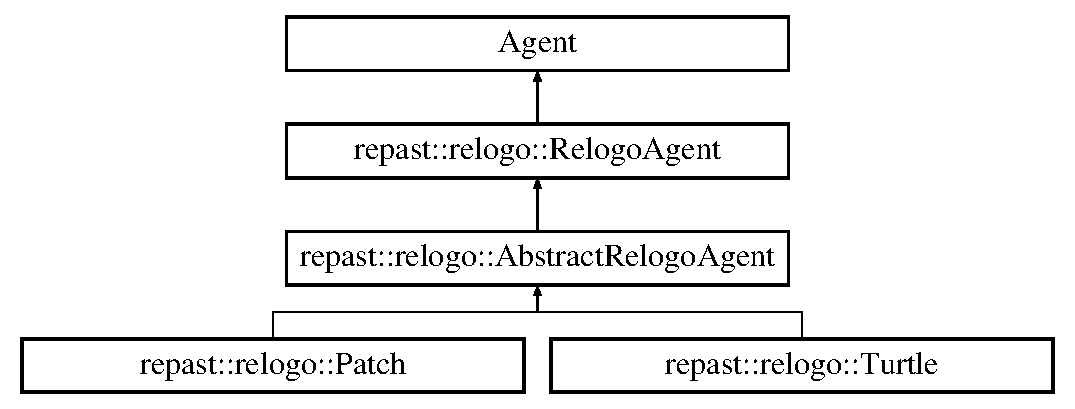
\includegraphics[height=4.000000cm]{classrepast_1_1relogo_1_1_abstract_relogo_agent}
\end{center}
\end{figure}
\subsection*{Public Member Functions}
\begin{DoxyCompactItemize}
\item 
\hypertarget{classrepast_1_1relogo_1_1_abstract_relogo_agent_a91a3e14db2e9b51270faf04cc24c6763}{{\bfseries Abstract\-Relogo\-Agent} (Agent\-Id id, \hyperlink{classrepast_1_1relogo_1_1_observer}{Observer} $\ast$observer)}\label{classrepast_1_1relogo_1_1_abstract_relogo_agent_a91a3e14db2e9b51270faf04cc24c6763}

\item 
virtual int \hyperlink{classrepast_1_1relogo_1_1_abstract_relogo_agent_ae631f45eba5815470dea5a2059213c1b}{px\-Cor} () const =0
\begin{DoxyCompactList}\small\item\em Gets the patch x coordinate of the agent's location. \end{DoxyCompactList}\item 
virtual int \hyperlink{classrepast_1_1relogo_1_1_abstract_relogo_agent_a38df42fbb6277fa62d0068fbd37e6595}{py\-Cor} () const =0
\begin{DoxyCompactList}\small\item\em Gets the patch y coordinate of the agent's location. \end{DoxyCompactList}\item 
{\footnotesize template$<$typename Agent\-Type $>$ }\\void \hyperlink{classrepast_1_1relogo_1_1_abstract_relogo_agent_aa166d2f1f0bd15ff4bf66afbc2575e6e}{in\-Radius} (\hyperlink{classrepast_1_1relogo_1_1_agent_set}{Agent\-Set}$<$ \hyperlink{classrepast_1_1relogo_1_1_relogo_agent}{Relogo\-Agent} $>$ \&in\-Set, double radius, \hyperlink{classrepast_1_1relogo_1_1_agent_set}{Agent\-Set}$<$ Agent\-Type $>$ \&out\-Set) const 
\begin{DoxyCompactList}\small\item\em Gets all the agents in the in\-Set within the specified radius for this \hyperlink{classrepast_1_1relogo_1_1_relogo_agent}{Relogo\-Agent} and put them in the out\-Set. \end{DoxyCompactList}\item 
{\footnotesize template$<$typename Patch\-Type $>$ }\\Patch\-Type $\ast$ \hyperlink{classrepast_1_1relogo_1_1_abstract_relogo_agent_abf11a5acb9ae1c549b4800abd8d2e2c9}{patch\-At} (double dx, double dy) const 
\begin{DoxyCompactList}\small\item\em Gets the patch at direction dx, dy from the this agent. \end{DoxyCompactList}\item 
{\footnotesize template$<$typename Agent\-Type $>$ }\\void \hyperlink{classrepast_1_1relogo_1_1_abstract_relogo_agent_aac0b1c2047d71efb46b99423b3ecb94b}{turtles\-Here} (\hyperlink{classrepast_1_1relogo_1_1_agent_set}{Agent\-Set}$<$ Agent\-Type $>$ \&set) const 
\begin{DoxyCompactList}\small\item\em Gets all the turtles on this turtle's patch and puts them into the specifed set. \end{DoxyCompactList}\item 
{\footnotesize template$<$typename Agent\-Type $>$ }\\\hyperlink{classrepast_1_1relogo_1_1_agent_set}{Agent\-Set}$<$ Agent\-Type $>$ \hyperlink{classrepast_1_1relogo_1_1_abstract_relogo_agent_a3bc15fe92588f63ad827a519137b98fc}{turtles\-Here} () const 
\begin{DoxyCompactList}\small\item\em Gets all the turtles on this turtle's patch and returns them in an \hyperlink{classrepast_1_1relogo_1_1_agent_set}{Agent\-Set}. \end{DoxyCompactList}\item 
{\footnotesize template$<$typename Patch\-Type $>$ }\\Patch\-Type $\ast$ \hyperlink{classrepast_1_1relogo_1_1_abstract_relogo_agent_ad06a915908d6a0597b707e458c1fd5de}{patch\-At\-Heading\-And\-Distance} (float heading, double \hyperlink{classrepast_1_1relogo_1_1_relogo_agent_a12a186ace28dcebf62faa6d3441f8a78}{distance})
\begin{DoxyCompactList}\small\item\em Gets the patch at the specified heading and distance from this patch or turtle. \end{DoxyCompactList}\item 
{\footnotesize template$<$typename Agent\-Type $>$ }\\void \hyperlink{classrepast_1_1relogo_1_1_abstract_relogo_agent_acf2f1f0e0acc8052de997140c8aadec8}{turtles\-On} (\hyperlink{classrepast_1_1relogo_1_1_agent_set}{Agent\-Set}$<$ Agent\-Type $>$ \&out) const 
\begin{DoxyCompactList}\small\item\em Gets the turtles that are on this patch or if this is a \hyperlink{classrepast_1_1relogo_1_1_turtle}{Turtle} get the turtles that are on the patch this turtle is on. \end{DoxyCompactList}\item 
{\footnotesize template$<$typename Agent\-Type $>$ }\\\hyperlink{classrepast_1_1relogo_1_1_agent_set}{Agent\-Set}$<$ Agent\-Type $>$ \hyperlink{classrepast_1_1relogo_1_1_abstract_relogo_agent_a851b68b9a35ae504fee0d416bd17ee0a}{turtles\-On} () const 
\begin{DoxyCompactList}\small\item\em Gets the turtles that are on this patch or if this is a \hyperlink{classrepast_1_1relogo_1_1_turtle}{Turtle} get the turtles that are on the patch this turtle is on. \end{DoxyCompactList}\end{DoxyCompactItemize}


\subsection{Detailed Description}
Abstract base class for turtles and patches. 

This contains some methods that can apply to either. 

\subsection{Member Function Documentation}
\hypertarget{classrepast_1_1relogo_1_1_abstract_relogo_agent_aa166d2f1f0bd15ff4bf66afbc2575e6e}{\index{repast\-::relogo\-::\-Abstract\-Relogo\-Agent@{repast\-::relogo\-::\-Abstract\-Relogo\-Agent}!in\-Radius@{in\-Radius}}
\index{in\-Radius@{in\-Radius}!repast::relogo::AbstractRelogoAgent@{repast\-::relogo\-::\-Abstract\-Relogo\-Agent}}
\subsubsection[{in\-Radius}]{\setlength{\rightskip}{0pt plus 5cm}template$<$typename Agent\-Type $>$ void repast\-::relogo\-::\-Abstract\-Relogo\-Agent\-::in\-Radius (
\begin{DoxyParamCaption}
\item[{{\bf Agent\-Set}$<$ {\bf Relogo\-Agent} $>$ \&}]{in\-Set, }
\item[{double}]{radius, }
\item[{{\bf Agent\-Set}$<$ Agent\-Type $>$ \&}]{out\-Set}
\end{DoxyParamCaption}
) const}}\label{classrepast_1_1relogo_1_1_abstract_relogo_agent_aa166d2f1f0bd15ff4bf66afbc2575e6e}


Gets all the agents in the in\-Set within the specified radius for this \hyperlink{classrepast_1_1relogo_1_1_relogo_agent}{Relogo\-Agent} and put them in the out\-Set. 


\begin{DoxyParams}{Parameters}
{\em in\-Set} & the set of agents to test if they are withinthe radius \\
\hline
\end{DoxyParams}

\begin{DoxyTemplParams}{Template Parameters}
{\em the} & type of agents to include in the out\-Set \\
\hline
\end{DoxyTemplParams}
\hypertarget{classrepast_1_1relogo_1_1_abstract_relogo_agent_abf11a5acb9ae1c549b4800abd8d2e2c9}{\index{repast\-::relogo\-::\-Abstract\-Relogo\-Agent@{repast\-::relogo\-::\-Abstract\-Relogo\-Agent}!patch\-At@{patch\-At}}
\index{patch\-At@{patch\-At}!repast::relogo::AbstractRelogoAgent@{repast\-::relogo\-::\-Abstract\-Relogo\-Agent}}
\subsubsection[{patch\-At}]{\setlength{\rightskip}{0pt plus 5cm}template$<$typename Patch\-Type $>$ Patch\-Type $\ast$ repast\-::relogo\-::\-Abstract\-Relogo\-Agent\-::patch\-At (
\begin{DoxyParamCaption}
\item[{double}]{dx, }
\item[{double}]{dy}
\end{DoxyParamCaption}
) const}}\label{classrepast_1_1relogo_1_1_abstract_relogo_agent_abf11a5acb9ae1c549b4800abd8d2e2c9}


Gets the patch at direction dx, dy from the this agent. 

If the resulting location is outside of the world, this returns 0.


\begin{DoxyParams}{Parameters}
{\em dx} & the distance from the caller along the x dimension \\
\hline
{\em dy} & the distance from the caller along the y dimension \\
\hline
\end{DoxyParams}

\begin{DoxyTemplParams}{Template Parameters}
{\em the} & type of the \hyperlink{classrepast_1_1relogo_1_1_patch}{Patch}\\
\hline
\end{DoxyTemplParams}
\begin{DoxyReturn}{Returns}
the patch at that distance from this \hyperlink{classrepast_1_1relogo_1_1_turtle}{Turtle}, or 0 if the resulting location is outside of the world. 
\end{DoxyReturn}
\hypertarget{classrepast_1_1relogo_1_1_abstract_relogo_agent_ad06a915908d6a0597b707e458c1fd5de}{\index{repast\-::relogo\-::\-Abstract\-Relogo\-Agent@{repast\-::relogo\-::\-Abstract\-Relogo\-Agent}!patch\-At\-Heading\-And\-Distance@{patch\-At\-Heading\-And\-Distance}}
\index{patch\-At\-Heading\-And\-Distance@{patch\-At\-Heading\-And\-Distance}!repast::relogo::AbstractRelogoAgent@{repast\-::relogo\-::\-Abstract\-Relogo\-Agent}}
\subsubsection[{patch\-At\-Heading\-And\-Distance}]{\setlength{\rightskip}{0pt plus 5cm}template$<$typename Patch\-Type $>$ Patch\-Type $\ast$ repast\-::relogo\-::\-Abstract\-Relogo\-Agent\-::patch\-At\-Heading\-And\-Distance (
\begin{DoxyParamCaption}
\item[{float}]{heading, }
\item[{double}]{distance}
\end{DoxyParamCaption}
)}}\label{classrepast_1_1relogo_1_1_abstract_relogo_agent_ad06a915908d6a0597b707e458c1fd5de}


Gets the patch at the specified heading and distance from this patch or turtle. 


\begin{DoxyParams}{Parameters}
{\em heading} & the heading \\
\hline
{\em distance} & the distance \\
\hline
\end{DoxyParams}

\begin{DoxyTemplParams}{Template Parameters}
{\em Patch\-Type} & the patch's type \\
\hline
\end{DoxyTemplParams}
\hypertarget{classrepast_1_1relogo_1_1_abstract_relogo_agent_ae631f45eba5815470dea5a2059213c1b}{\index{repast\-::relogo\-::\-Abstract\-Relogo\-Agent@{repast\-::relogo\-::\-Abstract\-Relogo\-Agent}!px\-Cor@{px\-Cor}}
\index{px\-Cor@{px\-Cor}!repast::relogo::AbstractRelogoAgent@{repast\-::relogo\-::\-Abstract\-Relogo\-Agent}}
\subsubsection[{px\-Cor}]{\setlength{\rightskip}{0pt plus 5cm}virtual int repast\-::relogo\-::\-Abstract\-Relogo\-Agent\-::px\-Cor (
\begin{DoxyParamCaption}
{}
\end{DoxyParamCaption}
) const\hspace{0.3cm}{\ttfamily [pure virtual]}}}\label{classrepast_1_1relogo_1_1_abstract_relogo_agent_ae631f45eba5815470dea5a2059213c1b}


Gets the patch x coordinate of the agent's location. 

\begin{DoxyReturn}{Returns}
the patch x coordinate 
\end{DoxyReturn}


Implements \hyperlink{classrepast_1_1relogo_1_1_relogo_agent_a8219a12f66709b4c86c547668235eda9}{repast\-::relogo\-::\-Relogo\-Agent}.



Implemented in \hyperlink{classrepast_1_1relogo_1_1_turtle_abeb7b773c8c9d403317587a7acdc1c1f}{repast\-::relogo\-::\-Turtle}, and \hyperlink{classrepast_1_1relogo_1_1_patch_a410a47c2b1dc260d83c65ffb66b33a75}{repast\-::relogo\-::\-Patch}.

\hypertarget{classrepast_1_1relogo_1_1_abstract_relogo_agent_a38df42fbb6277fa62d0068fbd37e6595}{\index{repast\-::relogo\-::\-Abstract\-Relogo\-Agent@{repast\-::relogo\-::\-Abstract\-Relogo\-Agent}!py\-Cor@{py\-Cor}}
\index{py\-Cor@{py\-Cor}!repast::relogo::AbstractRelogoAgent@{repast\-::relogo\-::\-Abstract\-Relogo\-Agent}}
\subsubsection[{py\-Cor}]{\setlength{\rightskip}{0pt plus 5cm}virtual int repast\-::relogo\-::\-Abstract\-Relogo\-Agent\-::py\-Cor (
\begin{DoxyParamCaption}
{}
\end{DoxyParamCaption}
) const\hspace{0.3cm}{\ttfamily [pure virtual]}}}\label{classrepast_1_1relogo_1_1_abstract_relogo_agent_a38df42fbb6277fa62d0068fbd37e6595}


Gets the patch y coordinate of the agent's location. 

\begin{DoxyReturn}{Returns}
the patch y coordinate 
\end{DoxyReturn}


Implements \hyperlink{classrepast_1_1relogo_1_1_relogo_agent_a4cf0eae31dc04149160dfd7b77044158}{repast\-::relogo\-::\-Relogo\-Agent}.



Implemented in \hyperlink{classrepast_1_1relogo_1_1_turtle_a378a3a80d2d33e389d8d78f0e0cae6d2}{repast\-::relogo\-::\-Turtle}, and \hyperlink{classrepast_1_1relogo_1_1_patch_a9fe953832fa384a6fa19bd32511954fc}{repast\-::relogo\-::\-Patch}.

\hypertarget{classrepast_1_1relogo_1_1_abstract_relogo_agent_aac0b1c2047d71efb46b99423b3ecb94b}{\index{repast\-::relogo\-::\-Abstract\-Relogo\-Agent@{repast\-::relogo\-::\-Abstract\-Relogo\-Agent}!turtles\-Here@{turtles\-Here}}
\index{turtles\-Here@{turtles\-Here}!repast::relogo::AbstractRelogoAgent@{repast\-::relogo\-::\-Abstract\-Relogo\-Agent}}
\subsubsection[{turtles\-Here}]{\setlength{\rightskip}{0pt plus 5cm}template$<$typename Agent\-Type $>$ void repast\-::relogo\-::\-Abstract\-Relogo\-Agent\-::turtles\-Here (
\begin{DoxyParamCaption}
\item[{{\bf Agent\-Set}$<$ Agent\-Type $>$ \&}]{set}
\end{DoxyParamCaption}
) const}}\label{classrepast_1_1relogo_1_1_abstract_relogo_agent_aac0b1c2047d71efb46b99423b3ecb94b}


Gets all the turtles on this turtle's patch and puts them into the specifed set. 


\begin{DoxyParams}{Parameters}
{\em set} & the set to put the found turtles in \\
\hline
\end{DoxyParams}

\begin{DoxyTemplParams}{Template Parameters}
{\em Agent\-Type} & the type of turtles to get \\
\hline
\end{DoxyTemplParams}
\hypertarget{classrepast_1_1relogo_1_1_abstract_relogo_agent_a3bc15fe92588f63ad827a519137b98fc}{\index{repast\-::relogo\-::\-Abstract\-Relogo\-Agent@{repast\-::relogo\-::\-Abstract\-Relogo\-Agent}!turtles\-Here@{turtles\-Here}}
\index{turtles\-Here@{turtles\-Here}!repast::relogo::AbstractRelogoAgent@{repast\-::relogo\-::\-Abstract\-Relogo\-Agent}}
\subsubsection[{turtles\-Here}]{\setlength{\rightskip}{0pt plus 5cm}template$<$typename Agent\-Type $>$ {\bf Agent\-Set}$<$ Agent\-Type $>$ repast\-::relogo\-::\-Abstract\-Relogo\-Agent\-::turtles\-Here (
\begin{DoxyParamCaption}
{}
\end{DoxyParamCaption}
) const}}\label{classrepast_1_1relogo_1_1_abstract_relogo_agent_a3bc15fe92588f63ad827a519137b98fc}


Gets all the turtles on this turtle's patch and returns them in an \hyperlink{classrepast_1_1relogo_1_1_agent_set}{Agent\-Set}. 


\begin{DoxyTemplParams}{Template Parameters}
{\em Agent\-Type} & the type of turtles to get\\
\hline
\end{DoxyTemplParams}
\begin{DoxyReturn}{Returns}
an \hyperlink{classrepast_1_1relogo_1_1_agent_set}{Agent\-Set} containing all the turtles on this turtles patch. 
\end{DoxyReturn}
\hypertarget{classrepast_1_1relogo_1_1_abstract_relogo_agent_acf2f1f0e0acc8052de997140c8aadec8}{\index{repast\-::relogo\-::\-Abstract\-Relogo\-Agent@{repast\-::relogo\-::\-Abstract\-Relogo\-Agent}!turtles\-On@{turtles\-On}}
\index{turtles\-On@{turtles\-On}!repast::relogo::AbstractRelogoAgent@{repast\-::relogo\-::\-Abstract\-Relogo\-Agent}}
\subsubsection[{turtles\-On}]{\setlength{\rightskip}{0pt plus 5cm}template$<$typename Agent\-Type $>$ void repast\-::relogo\-::\-Abstract\-Relogo\-Agent\-::turtles\-On (
\begin{DoxyParamCaption}
\item[{{\bf Agent\-Set}$<$ Agent\-Type $>$ \&}]{out}
\end{DoxyParamCaption}
) const}}\label{classrepast_1_1relogo_1_1_abstract_relogo_agent_acf2f1f0e0acc8052de997140c8aadec8}


Gets the turtles that are on this patch or if this is a \hyperlink{classrepast_1_1relogo_1_1_turtle}{Turtle} get the turtles that are on the patch this turtle is on. 


\begin{DoxyTemplParams}{Template Parameters}
{\em Agent\-Type} & the type of turtle \\
\hline
\end{DoxyTemplParams}

\begin{DoxyParams}{Parameters}
{\em out} & the turtles will be put in out \\
\hline
\end{DoxyParams}
\hypertarget{classrepast_1_1relogo_1_1_abstract_relogo_agent_a851b68b9a35ae504fee0d416bd17ee0a}{\index{repast\-::relogo\-::\-Abstract\-Relogo\-Agent@{repast\-::relogo\-::\-Abstract\-Relogo\-Agent}!turtles\-On@{turtles\-On}}
\index{turtles\-On@{turtles\-On}!repast::relogo::AbstractRelogoAgent@{repast\-::relogo\-::\-Abstract\-Relogo\-Agent}}
\subsubsection[{turtles\-On}]{\setlength{\rightskip}{0pt plus 5cm}template$<$typename Agent\-Type $>$ {\bf Agent\-Set}$<$ Agent\-Type $>$ repast\-::relogo\-::\-Abstract\-Relogo\-Agent\-::turtles\-On (
\begin{DoxyParamCaption}
{}
\end{DoxyParamCaption}
) const}}\label{classrepast_1_1relogo_1_1_abstract_relogo_agent_a851b68b9a35ae504fee0d416bd17ee0a}


Gets the turtles that are on this patch or if this is a \hyperlink{classrepast_1_1relogo_1_1_turtle}{Turtle} get the turtles that are on the patch this turtle is on. 


\begin{DoxyTemplParams}{Template Parameters}
{\em Agent\-Type} & the type of turtle\\
\hline
\end{DoxyTemplParams}
\begin{DoxyReturn}{Returns}
an \hyperlink{classrepast_1_1relogo_1_1_agent_set}{Agent\-Set} containing all the turtles that are on the patch the caller is on. 
\end{DoxyReturn}


The documentation for this class was generated from the following files\-:\begin{DoxyCompactItemize}
\item 
/\-Users/murphy/work/\-Repast\-H\-P\-C\-\_\-\-G\-I\-T/repast.\-hpc/src/relogo/Abstract\-Relogo\-Agent.\-h\item 
/\-Users/murphy/work/\-Repast\-H\-P\-C\-\_\-\-G\-I\-T/repast.\-hpc/src/relogo/Abstract\-Relogo\-Agent.\-cpp\end{DoxyCompactItemize}

\hypertarget{classrepast_1_1relogo_1_1_agent_set}{\section{repast\-:\-:relogo\-:\-:Agent\-Set$<$ T $>$ Class Template Reference}
\label{classrepast_1_1relogo_1_1_agent_set}\index{repast\-::relogo\-::\-Agent\-Set$<$ T $>$@{repast\-::relogo\-::\-Agent\-Set$<$ T $>$}}
}


Specialized indexable collection class for agents.  




{\ttfamily \#include $<$Agent\-Set.\-h$>$}

\subsection*{Public Types}
\begin{DoxyCompactItemize}
\item 
\hypertarget{classrepast_1_1relogo_1_1_agent_set_a6acda82cc586e441101f7dad92287d9e}{typedef std\-::vector$<$ T $\ast$ $>$\\*
\-::iterator {\bfseries as\-\_\-iterator}}\label{classrepast_1_1relogo_1_1_agent_set_a6acda82cc586e441101f7dad92287d9e}

\item 
\hypertarget{classrepast_1_1relogo_1_1_agent_set_adf53a71e8dcab04db9bbca40a1dfeba3}{typedef std\-::vector$<$ T $\ast$ $>$\\*
\-::const\-\_\-iterator {\bfseries const\-\_\-as\-\_\-iterator}}\label{classrepast_1_1relogo_1_1_agent_set_adf53a71e8dcab04db9bbca40a1dfeba3}

\end{DoxyCompactItemize}
\subsection*{Public Member Functions}
\begin{DoxyCompactItemize}
\item 
\hypertarget{classrepast_1_1relogo_1_1_agent_set_a57e45513bb2fee478ceba906c563fa42}{\hyperlink{classrepast_1_1relogo_1_1_agent_set_a57e45513bb2fee478ceba906c563fa42}{Agent\-Set} ()}\label{classrepast_1_1relogo_1_1_agent_set_a57e45513bb2fee478ceba906c563fa42}

\begin{DoxyCompactList}\small\item\em Creates an empty agent set. \end{DoxyCompactList}\item 
\hypertarget{classrepast_1_1relogo_1_1_agent_set_ad05a9d50cb9c512fd399758fa3d141f0}{{\footnotesize template$<$typename input\-\_\-iterator $>$ }\\\hyperlink{classrepast_1_1relogo_1_1_agent_set_ad05a9d50cb9c512fd399758fa3d141f0}{Agent\-Set} (input\-\_\-iterator start, input\-\_\-iterator \hyperlink{classrepast_1_1relogo_1_1_agent_set_ab862376938b785f091c0b0720de759f3}{end})}\label{classrepast_1_1relogo_1_1_agent_set_ad05a9d50cb9c512fd399758fa3d141f0}

\begin{DoxyCompactList}\small\item\em Creates an agent set and fills with elements from start through end. \end{DoxyCompactList}\item 
\hypertarget{classrepast_1_1relogo_1_1_agent_set_a667732a4a0d7a49ca57c8f8373bb979c}{\hyperlink{classrepast_1_1relogo_1_1_agent_set_a667732a4a0d7a49ca57c8f8373bb979c}{Agent\-Set} (const \hyperlink{classrepast_1_1relogo_1_1_agent_set}{Agent\-Set} \&set)}\label{classrepast_1_1relogo_1_1_agent_set_a667732a4a0d7a49ca57c8f8373bb979c}

\begin{DoxyCompactList}\small\item\em Copy constructor. \end{DoxyCompactList}\item 
\hypertarget{classrepast_1_1relogo_1_1_agent_set_afc89da64293d944f23cb36d41e146f9e}{{\footnotesize template$<$typename input\-\_\-iterator $>$ }\\void \hyperlink{classrepast_1_1relogo_1_1_agent_set_afc89da64293d944f23cb36d41e146f9e}{add\-All} (input\-\_\-iterator \hyperlink{classrepast_1_1relogo_1_1_agent_set_a9492708e0f156e29fcfa77f9477887af}{begin}, input\-\_\-iterator \hyperlink{classrepast_1_1relogo_1_1_agent_set_ab862376938b785f091c0b0720de759f3}{end})}\label{classrepast_1_1relogo_1_1_agent_set_afc89da64293d944f23cb36d41e146f9e}

\begin{DoxyCompactList}\small\item\em Adds all the agents from the start iterator through the end to this \hyperlink{classrepast_1_1relogo_1_1_agent_set}{Agent\-Set}. \end{DoxyCompactList}\item 
\hypertarget{classrepast_1_1relogo_1_1_agent_set_a2b06374a28dd6ee8d7d9c8a7ebf8d8a8}{void \hyperlink{classrepast_1_1relogo_1_1_agent_set_a2b06374a28dd6ee8d7d9c8a7ebf8d8a8}{add} (T $\ast$agent)}\label{classrepast_1_1relogo_1_1_agent_set_a2b06374a28dd6ee8d7d9c8a7ebf8d8a8}

\begin{DoxyCompactList}\small\item\em Adds an agent to this \hyperlink{classrepast_1_1relogo_1_1_agent_set}{Agent\-Set}. \end{DoxyCompactList}\item 
{\footnotesize template$<$typename Functor $>$ }\\void \hyperlink{classrepast_1_1relogo_1_1_agent_set_a5caff8a45e775403881012e105030134}{ask} (Functor func)
\begin{DoxyCompactList}\small\item\em Calls the Functor on each agent in this \hyperlink{classrepast_1_1relogo_1_1_agent_set}{Agent\-Set}. \end{DoxyCompactList}\item 
{\footnotesize template$<$typename Functor , typename P1 $>$ }\\void \hyperlink{classrepast_1_1relogo_1_1_agent_set_a21561fa480f0dbaa059753815fbe7821}{ask} (Functor func, const P1 \&p1)
\begin{DoxyCompactList}\small\item\em Calls the Functor on each agent in this \hyperlink{classrepast_1_1relogo_1_1_agent_set}{Agent\-Set}, passing the specified argument. \end{DoxyCompactList}\item 
{\footnotesize template$<$typename Functor , typename P1 $>$ }\\void \hyperlink{classrepast_1_1relogo_1_1_agent_set_a2af4658a4ca1205fba7225064d736d42}{ask} (Functor func, P1 \&p1)
\begin{DoxyCompactList}\small\item\em Calls the Functor on each agent in this \hyperlink{classrepast_1_1relogo_1_1_agent_set}{Agent\-Set}, passing the specified argument. \end{DoxyCompactList}\item 
{\footnotesize template$<$typename Functor $>$ }\\void \hyperlink{classrepast_1_1relogo_1_1_agent_set_ad3598fac70650951640e6c114139ae3b}{apply} (Functor \&func)
\begin{DoxyCompactList}\small\item\em Applies the functor to each each agent in the agent set. \end{DoxyCompactList}\item 
{\footnotesize template$<$typename Functor $>$ }\\void \hyperlink{classrepast_1_1relogo_1_1_agent_set_a7504d1d703d7fa46ce159a4d1b2f59fc}{apply} (const Functor \&func)
\begin{DoxyCompactList}\small\item\em Applies the functor to each each agent in the agent set. \end{DoxyCompactList}\item 
T $\ast$ \hyperlink{classrepast_1_1relogo_1_1_agent_set_a2c6200d20ec50279d5e52ffedd8f763e}{at} (int index)
\begin{DoxyCompactList}\small\item\em Gets the item at the specified index. \end{DoxyCompactList}\item 
size\-\_\-t \hyperlink{classrepast_1_1relogo_1_1_agent_set_aa3a44b933b292416299f4da0ce39d0ae}{count} () const 
\begin{DoxyCompactList}\small\item\em Gets the size of this \hyperlink{classrepast_1_1relogo_1_1_agent_set}{Agent\-Set}. \end{DoxyCompactList}\item 
size\-\_\-t \hyperlink{classrepast_1_1relogo_1_1_agent_set_abb4a6f94c42cf89dff6f08f1eb47ab51}{size} () const 
\begin{DoxyCompactList}\small\item\em Gets the size of this \hyperlink{classrepast_1_1relogo_1_1_agent_set}{Agent\-Set}. \end{DoxyCompactList}\item 
T $\ast$ \hyperlink{classrepast_1_1relogo_1_1_agent_set_a7a0f373b6f05f4d01a9eaff067b7d514}{operator\mbox{[}$\,$\mbox{]}} (size\-\_\-t index)
\begin{DoxyCompactList}\small\item\em Gets the item at the specified index without doing any range checking. \end{DoxyCompactList}\item 
as\-\_\-iterator \hyperlink{classrepast_1_1relogo_1_1_agent_set_a9492708e0f156e29fcfa77f9477887af}{begin} ()
\begin{DoxyCompactList}\small\item\em Gets an iterator to the begining of this \hyperlink{classrepast_1_1relogo_1_1_agent_set}{Agent\-Set}. \end{DoxyCompactList}\item 
const\-\_\-as\-\_\-iterator \hyperlink{classrepast_1_1relogo_1_1_agent_set_a209b06bdddbcf48eebc316c7784c226c}{begin} () const 
\begin{DoxyCompactList}\small\item\em Gets a const iterator to the begining of this \hyperlink{classrepast_1_1relogo_1_1_agent_set}{Agent\-Set}. \end{DoxyCompactList}\item 
as\-\_\-iterator \hyperlink{classrepast_1_1relogo_1_1_agent_set_ab862376938b785f091c0b0720de759f3}{end} ()
\begin{DoxyCompactList}\small\item\em Gets an iterator to the end of this \hyperlink{classrepast_1_1relogo_1_1_agent_set}{Agent\-Set}. \end{DoxyCompactList}\item 
const\-\_\-as\-\_\-iterator \hyperlink{classrepast_1_1relogo_1_1_agent_set_a9b48798c03c4a1f39d63af9a0efefc96}{end} () const 
\begin{DoxyCompactList}\small\item\em Gets a const iterator to the end of this \hyperlink{classrepast_1_1relogo_1_1_agent_set}{Agent\-Set}. \end{DoxyCompactList}\item 
\hypertarget{classrepast_1_1relogo_1_1_agent_set_aad1e6bd07bd986979044c1097464de19}{void \hyperlink{classrepast_1_1relogo_1_1_agent_set_aad1e6bd07bd986979044c1097464de19}{clear} ()}\label{classrepast_1_1relogo_1_1_agent_set_aad1e6bd07bd986979044c1097464de19}

\begin{DoxyCompactList}\small\item\em Clears this \hyperlink{classrepast_1_1relogo_1_1_agent_set}{Agent\-Set} of any agents that it contains. \end{DoxyCompactList}\item 
{\footnotesize template$<$typename Value\-Getter $>$ }\\T $\ast$ \hyperlink{classrepast_1_1relogo_1_1_agent_set_af51f6858bfa282b98803663fd98ee586}{min\-One\-Of} (const Value\-Getter \&getter)
\begin{DoxyCompactList}\small\item\em Gets the set member that has the minimum value of the number returned by Value\-Getter. \end{DoxyCompactList}\item 
{\footnotesize template$<$typename Value\-Getter $>$ }\\T $\ast$ \hyperlink{classrepast_1_1relogo_1_1_agent_set_a3ee8b550f0157ae73c0bd9b63debef14}{max\-One\-Of} (const Value\-Getter \&getter)
\begin{DoxyCompactList}\small\item\em Gets the set member that has the maximum value of the number returned by Value\-Getter. \end{DoxyCompactList}\item 
{\footnotesize template$<$typename Value\-Getter $>$ }\\void \hyperlink{classrepast_1_1relogo_1_1_agent_set_a56e27a6154a3bb13310a8e4e9e7e75ab}{with\-Min} (const Value\-Getter \&getter, \hyperlink{classrepast_1_1relogo_1_1_agent_set}{Agent\-Set}$<$ T $>$ \&set)
\begin{DoxyCompactList}\small\item\em Gets the set members that have the minimum value of the number returned by Value\-Getter, and puts them in the specified set. \end{DoxyCompactList}\item 
{\footnotesize template$<$typename Value\-Getter $>$ }\\void \hyperlink{classrepast_1_1relogo_1_1_agent_set_a3a1086c427446de2b5587a442b044a01}{with\-Max} (const Value\-Getter \&getter, \hyperlink{classrepast_1_1relogo_1_1_agent_set}{Agent\-Set}$<$ T $>$ \&set)
\begin{DoxyCompactList}\small\item\em Gets the set members that have the maximum value of the number returned by Value\-Getter and puts them in the specified set. \end{DoxyCompactList}\item 
{\footnotesize template$<$typename Value\-Getter $>$ }\\void \hyperlink{classrepast_1_1relogo_1_1_agent_set_a7c148ed677ad6f2f1db3d56fd644adf2}{min\-N\-Of} (size\-\_\-t \hyperlink{classrepast_1_1relogo_1_1_agent_set_aa3a44b933b292416299f4da0ce39d0ae}{count}, const Value\-Getter \&getter, \hyperlink{classrepast_1_1relogo_1_1_agent_set}{Agent\-Set}$<$ T $>$ \&set, bool initial\-Set\-Is\-Sorted=false)
\begin{DoxyCompactList}\small\item\em Gets count number of set members that have the minimum value of the number returned by Value\-Getter. \end{DoxyCompactList}\item 
{\footnotesize template$<$typename Value\-Getter $>$ }\\void \hyperlink{classrepast_1_1relogo_1_1_agent_set_ae572019108c57f8a8d4e9dcd5feddd42}{max\-N\-Of} (size\-\_\-t \hyperlink{classrepast_1_1relogo_1_1_agent_set_aa3a44b933b292416299f4da0ce39d0ae}{count}, const Value\-Getter \&getter, \hyperlink{classrepast_1_1relogo_1_1_agent_set}{Agent\-Set}$<$ T $>$ \&set, bool initial\-Set\-Is\-Sorted=false)
\begin{DoxyCompactList}\small\item\em Gets count number of set members that have the maximum value of the number returned by Value\-Getter. \end{DoxyCompactList}\item 
T $\ast$ \hyperlink{classrepast_1_1relogo_1_1_agent_set_a86c9434e990506cc04975062eaa9235c}{one\-Of} ()
\begin{DoxyCompactList}\small\item\em Gets one of the members of this \hyperlink{classrepast_1_1relogo_1_1_agent_set}{Agent\-Set} at random. \end{DoxyCompactList}\item 
\hypertarget{classrepast_1_1relogo_1_1_agent_set_a71cc2d2b676bce1728d3e8a7a9d2a96a}{void \hyperlink{classrepast_1_1relogo_1_1_agent_set_a71cc2d2b676bce1728d3e8a7a9d2a96a}{remove} (T $\ast$agent)}\label{classrepast_1_1relogo_1_1_agent_set_a71cc2d2b676bce1728d3e8a7a9d2a96a}

\begin{DoxyCompactList}\small\item\em Removes all instances of the specified agent from this \hyperlink{classrepast_1_1relogo_1_1_agent_set}{Agent\-Set}. \end{DoxyCompactList}\item 
\hypertarget{classrepast_1_1relogo_1_1_agent_set_ab3ba8ae249e8b09b37b5f5005c725ce1}{void \hyperlink{classrepast_1_1relogo_1_1_agent_set_ab3ba8ae249e8b09b37b5f5005c725ce1}{shuffle} ()}\label{classrepast_1_1relogo_1_1_agent_set_ab3ba8ae249e8b09b37b5f5005c725ce1}

\begin{DoxyCompactList}\small\item\em Randomly shuffles the elements of this \hyperlink{classrepast_1_1relogo_1_1_agent_set}{Agent\-Set}. \end{DoxyCompactList}\end{DoxyCompactItemize}
\subsection*{Public Attributes}
\begin{DoxyCompactItemize}
\item 
\hypertarget{classrepast_1_1relogo_1_1_agent_set_a8bfb57ea4d61d60810b354645b013761}{std\-::vector$<$ T $\ast$ $>$ {\bfseries agents}}\label{classrepast_1_1relogo_1_1_agent_set_a8bfb57ea4d61d60810b354645b013761}

\end{DoxyCompactItemize}


\subsection{Detailed Description}
\subsubsection*{template$<$typename T$>$class repast\-::relogo\-::\-Agent\-Set$<$ T $>$}

Specialized indexable collection class for agents. 

This includes methods designed to call arbitrary code on the agents it contains.


\begin{DoxyTemplParams}{Template Parameters}
{\em T} & the type of agent the \hyperlink{classrepast_1_1relogo_1_1_agent_set}{Agent\-Set} contains \\
\hline
\end{DoxyTemplParams}


\subsection{Member Function Documentation}
\hypertarget{classrepast_1_1relogo_1_1_agent_set_ad3598fac70650951640e6c114139ae3b}{\index{repast\-::relogo\-::\-Agent\-Set@{repast\-::relogo\-::\-Agent\-Set}!apply@{apply}}
\index{apply@{apply}!repast::relogo::AgentSet@{repast\-::relogo\-::\-Agent\-Set}}
\subsubsection[{apply}]{\setlength{\rightskip}{0pt plus 5cm}template$<$typename T $>$ template$<$typename Functor $>$ void {\bf repast\-::relogo\-::\-Agent\-Set}$<$ T $>$\-::apply (
\begin{DoxyParamCaption}
\item[{Functor \&}]{func}
\end{DoxyParamCaption}
)}}\label{classrepast_1_1relogo_1_1_agent_set_ad3598fac70650951640e6c114139ae3b}


Applies the functor to each each agent in the agent set. 


\begin{DoxyTemplParams}{Template Parameters}
{\em Functor} & an object that implements operator()(\-T$\ast$ agent); \\
\hline
\end{DoxyTemplParams}
\hypertarget{classrepast_1_1relogo_1_1_agent_set_a7504d1d703d7fa46ce159a4d1b2f59fc}{\index{repast\-::relogo\-::\-Agent\-Set@{repast\-::relogo\-::\-Agent\-Set}!apply@{apply}}
\index{apply@{apply}!repast::relogo::AgentSet@{repast\-::relogo\-::\-Agent\-Set}}
\subsubsection[{apply}]{\setlength{\rightskip}{0pt plus 5cm}template$<$typename T $>$ template$<$typename Functor $>$ void {\bf repast\-::relogo\-::\-Agent\-Set}$<$ T $>$\-::apply (
\begin{DoxyParamCaption}
\item[{const Functor \&}]{func}
\end{DoxyParamCaption}
)}}\label{classrepast_1_1relogo_1_1_agent_set_a7504d1d703d7fa46ce159a4d1b2f59fc}


Applies the functor to each each agent in the agent set. 


\begin{DoxyTemplParams}{Template Parameters}
{\em Functor} & an object that implements operator()(\-T$\ast$ agent); \\
\hline
\end{DoxyTemplParams}
\hypertarget{classrepast_1_1relogo_1_1_agent_set_a5caff8a45e775403881012e105030134}{\index{repast\-::relogo\-::\-Agent\-Set@{repast\-::relogo\-::\-Agent\-Set}!ask@{ask}}
\index{ask@{ask}!repast::relogo::AgentSet@{repast\-::relogo\-::\-Agent\-Set}}
\subsubsection[{ask}]{\setlength{\rightskip}{0pt plus 5cm}template$<$typename T $>$ template$<$typename Functor $>$ void {\bf repast\-::relogo\-::\-Agent\-Set}$<$ T $>$\-::ask (
\begin{DoxyParamCaption}
\item[{Functor}]{func}
\end{DoxyParamCaption}
)}}\label{classrepast_1_1relogo_1_1_agent_set_a5caff8a45e775403881012e105030134}


Calls the Functor on each agent in this \hyperlink{classrepast_1_1relogo_1_1_agent_set}{Agent\-Set}. 


\begin{DoxyParams}{Parameters}
{\em func} & a pointer to the method to call each member of the set\\
\hline
\end{DoxyParams}

\begin{DoxyTemplParams}{Template Parameters}
{\em Functor} & pointer to no-\/arg method belonging to the type of agent contained by this \hyperlink{classrepast_1_1relogo_1_1_agent_set}{Agent\-Set}. \\
\hline
\end{DoxyTemplParams}
\hypertarget{classrepast_1_1relogo_1_1_agent_set_a21561fa480f0dbaa059753815fbe7821}{\index{repast\-::relogo\-::\-Agent\-Set@{repast\-::relogo\-::\-Agent\-Set}!ask@{ask}}
\index{ask@{ask}!repast::relogo::AgentSet@{repast\-::relogo\-::\-Agent\-Set}}
\subsubsection[{ask}]{\setlength{\rightskip}{0pt plus 5cm}template$<$typename T $>$ template$<$typename Functor , typename P1 $>$ void {\bf repast\-::relogo\-::\-Agent\-Set}$<$ T $>$\-::ask (
\begin{DoxyParamCaption}
\item[{Functor}]{func, }
\item[{const P1 \&}]{p1}
\end{DoxyParamCaption}
)}}\label{classrepast_1_1relogo_1_1_agent_set_a21561fa480f0dbaa059753815fbe7821}


Calls the Functor on each agent in this \hyperlink{classrepast_1_1relogo_1_1_agent_set}{Agent\-Set}, passing the specified argument. 


\begin{DoxyParams}{Parameters}
{\em func} & a pointer to the method to call each member of the set \\
\hline
{\em p1} & a reference to a P1 type that is passed to the called method\\
\hline
\end{DoxyParams}

\begin{DoxyTemplParams}{Template Parameters}
{\em Functor} & pointer to method belonging to the type of agent contained by this \hyperlink{classrepast_1_1relogo_1_1_agent_set}{Agent\-Set}. \\
\hline
{\em P1} & the type of the method parameter \\
\hline
\end{DoxyTemplParams}
\hypertarget{classrepast_1_1relogo_1_1_agent_set_a2af4658a4ca1205fba7225064d736d42}{\index{repast\-::relogo\-::\-Agent\-Set@{repast\-::relogo\-::\-Agent\-Set}!ask@{ask}}
\index{ask@{ask}!repast::relogo::AgentSet@{repast\-::relogo\-::\-Agent\-Set}}
\subsubsection[{ask}]{\setlength{\rightskip}{0pt plus 5cm}template$<$typename T $>$ template$<$typename Functor , typename P1 $>$ void {\bf repast\-::relogo\-::\-Agent\-Set}$<$ T $>$\-::ask (
\begin{DoxyParamCaption}
\item[{Functor}]{func, }
\item[{P1 \&}]{p1}
\end{DoxyParamCaption}
)}}\label{classrepast_1_1relogo_1_1_agent_set_a2af4658a4ca1205fba7225064d736d42}


Calls the Functor on each agent in this \hyperlink{classrepast_1_1relogo_1_1_agent_set}{Agent\-Set}, passing the specified argument. 


\begin{DoxyParams}{Parameters}
{\em func} & a pointer to the method to call each member of the set \\
\hline
{\em p1} & a reference to a P1 type that is passed to the called method \\
\hline
\end{DoxyParams}

\begin{DoxyTemplParams}{Template Parameters}
{\em Functor} & pointer to method belonging to the type of agent contained by this \hyperlink{classrepast_1_1relogo_1_1_agent_set}{Agent\-Set}. \\
\hline
{\em P1} & the type of the method parameter \\
\hline
\end{DoxyTemplParams}
\hypertarget{classrepast_1_1relogo_1_1_agent_set_a2c6200d20ec50279d5e52ffedd8f763e}{\index{repast\-::relogo\-::\-Agent\-Set@{repast\-::relogo\-::\-Agent\-Set}!at@{at}}
\index{at@{at}!repast::relogo::AgentSet@{repast\-::relogo\-::\-Agent\-Set}}
\subsubsection[{at}]{\setlength{\rightskip}{0pt plus 5cm}template$<$typename T $>$ T $\ast$ {\bf repast\-::relogo\-::\-Agent\-Set}$<$ T $>$\-::at (
\begin{DoxyParamCaption}
\item[{int}]{index}
\end{DoxyParamCaption}
)}}\label{classrepast_1_1relogo_1_1_agent_set_a2c6200d20ec50279d5e52ffedd8f763e}


Gets the item at the specified index. 


\begin{DoxyParams}{Parameters}
{\em index} & the index of the agent to get \\
\hline
\end{DoxyParams}
\begin{DoxyReturn}{Returns}
the agent at the specified index 
\end{DoxyReturn}
\hypertarget{classrepast_1_1relogo_1_1_agent_set_a9492708e0f156e29fcfa77f9477887af}{\index{repast\-::relogo\-::\-Agent\-Set@{repast\-::relogo\-::\-Agent\-Set}!begin@{begin}}
\index{begin@{begin}!repast::relogo::AgentSet@{repast\-::relogo\-::\-Agent\-Set}}
\subsubsection[{begin}]{\setlength{\rightskip}{0pt plus 5cm}template$<$typename T$>$ as\-\_\-iterator {\bf repast\-::relogo\-::\-Agent\-Set}$<$ T $>$\-::begin (
\begin{DoxyParamCaption}
{}
\end{DoxyParamCaption}
)\hspace{0.3cm}{\ttfamily [inline]}}}\label{classrepast_1_1relogo_1_1_agent_set_a9492708e0f156e29fcfa77f9477887af}


Gets an iterator to the begining of this \hyperlink{classrepast_1_1relogo_1_1_agent_set}{Agent\-Set}. 

\begin{DoxyReturn}{Returns}
an iterator to the beginning of this \hyperlink{classrepast_1_1relogo_1_1_agent_set}{Agent\-Set}. 
\end{DoxyReturn}
\hypertarget{classrepast_1_1relogo_1_1_agent_set_a209b06bdddbcf48eebc316c7784c226c}{\index{repast\-::relogo\-::\-Agent\-Set@{repast\-::relogo\-::\-Agent\-Set}!begin@{begin}}
\index{begin@{begin}!repast::relogo::AgentSet@{repast\-::relogo\-::\-Agent\-Set}}
\subsubsection[{begin}]{\setlength{\rightskip}{0pt plus 5cm}template$<$typename T$>$ const\-\_\-as\-\_\-iterator {\bf repast\-::relogo\-::\-Agent\-Set}$<$ T $>$\-::begin (
\begin{DoxyParamCaption}
{}
\end{DoxyParamCaption}
) const\hspace{0.3cm}{\ttfamily [inline]}}}\label{classrepast_1_1relogo_1_1_agent_set_a209b06bdddbcf48eebc316c7784c226c}


Gets a const iterator to the begining of this \hyperlink{classrepast_1_1relogo_1_1_agent_set}{Agent\-Set}. 

\begin{DoxyReturn}{Returns}
a const iterator to the beginning of this \hyperlink{classrepast_1_1relogo_1_1_agent_set}{Agent\-Set}. 
\end{DoxyReturn}
\hypertarget{classrepast_1_1relogo_1_1_agent_set_aa3a44b933b292416299f4da0ce39d0ae}{\index{repast\-::relogo\-::\-Agent\-Set@{repast\-::relogo\-::\-Agent\-Set}!count@{count}}
\index{count@{count}!repast::relogo::AgentSet@{repast\-::relogo\-::\-Agent\-Set}}
\subsubsection[{count}]{\setlength{\rightskip}{0pt plus 5cm}template$<$typename T$>$ size\-\_\-t {\bf repast\-::relogo\-::\-Agent\-Set}$<$ T $>$\-::count (
\begin{DoxyParamCaption}
{}
\end{DoxyParamCaption}
) const\hspace{0.3cm}{\ttfamily [inline]}}}\label{classrepast_1_1relogo_1_1_agent_set_aa3a44b933b292416299f4da0ce39d0ae}


Gets the size of this \hyperlink{classrepast_1_1relogo_1_1_agent_set}{Agent\-Set}. 

\begin{DoxyReturn}{Returns}
the size of this \hyperlink{classrepast_1_1relogo_1_1_agent_set}{Agent\-Set}. 
\end{DoxyReturn}
\hypertarget{classrepast_1_1relogo_1_1_agent_set_ab862376938b785f091c0b0720de759f3}{\index{repast\-::relogo\-::\-Agent\-Set@{repast\-::relogo\-::\-Agent\-Set}!end@{end}}
\index{end@{end}!repast::relogo::AgentSet@{repast\-::relogo\-::\-Agent\-Set}}
\subsubsection[{end}]{\setlength{\rightskip}{0pt plus 5cm}template$<$typename T$>$ as\-\_\-iterator {\bf repast\-::relogo\-::\-Agent\-Set}$<$ T $>$\-::end (
\begin{DoxyParamCaption}
{}
\end{DoxyParamCaption}
)\hspace{0.3cm}{\ttfamily [inline]}}}\label{classrepast_1_1relogo_1_1_agent_set_ab862376938b785f091c0b0720de759f3}


Gets an iterator to the end of this \hyperlink{classrepast_1_1relogo_1_1_agent_set}{Agent\-Set}. 

\begin{DoxyReturn}{Returns}
an iterator to the end of this \hyperlink{classrepast_1_1relogo_1_1_agent_set}{Agent\-Set}. 
\end{DoxyReturn}
\hypertarget{classrepast_1_1relogo_1_1_agent_set_a9b48798c03c4a1f39d63af9a0efefc96}{\index{repast\-::relogo\-::\-Agent\-Set@{repast\-::relogo\-::\-Agent\-Set}!end@{end}}
\index{end@{end}!repast::relogo::AgentSet@{repast\-::relogo\-::\-Agent\-Set}}
\subsubsection[{end}]{\setlength{\rightskip}{0pt plus 5cm}template$<$typename T$>$ const\-\_\-as\-\_\-iterator {\bf repast\-::relogo\-::\-Agent\-Set}$<$ T $>$\-::end (
\begin{DoxyParamCaption}
{}
\end{DoxyParamCaption}
) const\hspace{0.3cm}{\ttfamily [inline]}}}\label{classrepast_1_1relogo_1_1_agent_set_a9b48798c03c4a1f39d63af9a0efefc96}


Gets a const iterator to the end of this \hyperlink{classrepast_1_1relogo_1_1_agent_set}{Agent\-Set}. 

\begin{DoxyReturn}{Returns}
a const iterator to the end of this \hyperlink{classrepast_1_1relogo_1_1_agent_set}{Agent\-Set}. 
\end{DoxyReturn}
\hypertarget{classrepast_1_1relogo_1_1_agent_set_ae572019108c57f8a8d4e9dcd5feddd42}{\index{repast\-::relogo\-::\-Agent\-Set@{repast\-::relogo\-::\-Agent\-Set}!max\-N\-Of@{max\-N\-Of}}
\index{max\-N\-Of@{max\-N\-Of}!repast::relogo::AgentSet@{repast\-::relogo\-::\-Agent\-Set}}
\subsubsection[{max\-N\-Of}]{\setlength{\rightskip}{0pt plus 5cm}template$<$typename T $>$ template$<$typename Value\-Getter $>$ void {\bf repast\-::relogo\-::\-Agent\-Set}$<$ T $>$\-::max\-N\-Of (
\begin{DoxyParamCaption}
\item[{size\-\_\-t}]{count, }
\item[{const Value\-Getter \&}]{getter, }
\item[{{\bf Agent\-Set}$<$ T $>$ \&}]{set, }
\item[{bool}]{initial\-Set\-Is\-Sorted = {\ttfamily false}}
\end{DoxyParamCaption}
)}}\label{classrepast_1_1relogo_1_1_agent_set_ae572019108c57f8a8d4e9dcd5feddd42}


Gets count number of set members that have the maximum value of the number returned by Value\-Getter. 

If there are not enough to satisfy the count then members with the second lowest value are returned and so on.


\begin{DoxyParams}{Parameters}
{\em getter} & the Value\-Getter to use in retreiving the value used in the max comparison\\
\hline
\end{DoxyParams}

\begin{DoxyTemplParams}{Template Parameters}
{\em Value\-Getter} & a function or functor that takes a member of this agentset and returns a double value. This double value is used in the max comparison. \\
\hline
\end{DoxyTemplParams}

\begin{DoxyParams}{Parameters}
{\em initial\-Set\-Is\-Sorted} & Optional performance parameter; if false (the default), a call to this function must sort an entire copy of the original set; if true, the function assumes the original set is already sorted. Useful if the same set is to be used repeatedly. \\
\hline
\end{DoxyParams}
\hypertarget{classrepast_1_1relogo_1_1_agent_set_a3ee8b550f0157ae73c0bd9b63debef14}{\index{repast\-::relogo\-::\-Agent\-Set@{repast\-::relogo\-::\-Agent\-Set}!max\-One\-Of@{max\-One\-Of}}
\index{max\-One\-Of@{max\-One\-Of}!repast::relogo::AgentSet@{repast\-::relogo\-::\-Agent\-Set}}
\subsubsection[{max\-One\-Of}]{\setlength{\rightskip}{0pt plus 5cm}template$<$typename T $>$ template$<$typename Value\-Getter $>$ T $\ast$ {\bf repast\-::relogo\-::\-Agent\-Set}$<$ T $>$\-::max\-One\-Of (
\begin{DoxyParamCaption}
\item[{const Value\-Getter \&}]{getter}
\end{DoxyParamCaption}
)}}\label{classrepast_1_1relogo_1_1_agent_set_a3ee8b550f0157ae73c0bd9b63debef14}


Gets the set member that has the maximum value of the number returned by Value\-Getter. 

If more than one agent has the minimum value, then return one of those at random.


\begin{DoxyParams}{Parameters}
{\em getter} & the Value\-Getter to use in retreiving the value used in the max comparison\\
\hline
\end{DoxyParams}

\begin{DoxyTemplParams}{Template Parameters}
{\em Value\-Getter} & a function or functor that takes a member of this agentset and returns a double value. This double value is used in the max comparison. \\
\hline
\end{DoxyTemplParams}
\hypertarget{classrepast_1_1relogo_1_1_agent_set_a7c148ed677ad6f2f1db3d56fd644adf2}{\index{repast\-::relogo\-::\-Agent\-Set@{repast\-::relogo\-::\-Agent\-Set}!min\-N\-Of@{min\-N\-Of}}
\index{min\-N\-Of@{min\-N\-Of}!repast::relogo::AgentSet@{repast\-::relogo\-::\-Agent\-Set}}
\subsubsection[{min\-N\-Of}]{\setlength{\rightskip}{0pt plus 5cm}template$<$typename T $>$ template$<$typename Value\-Getter $>$ void {\bf repast\-::relogo\-::\-Agent\-Set}$<$ T $>$\-::min\-N\-Of (
\begin{DoxyParamCaption}
\item[{size\-\_\-t}]{count, }
\item[{const Value\-Getter \&}]{getter, }
\item[{{\bf Agent\-Set}$<$ T $>$ \&}]{set, }
\item[{bool}]{initial\-Set\-Is\-Sorted = {\ttfamily false}}
\end{DoxyParamCaption}
)}}\label{classrepast_1_1relogo_1_1_agent_set_a7c148ed677ad6f2f1db3d56fd644adf2}


Gets count number of set members that have the minimum value of the number returned by Value\-Getter. 

If there are not enough to satisfy the count then members with the second lowest value are returned and so on.


\begin{DoxyParams}{Parameters}
{\em getter} & the Value\-Getter to use in retreiving the value used in the min comparison\\
\hline
\end{DoxyParams}

\begin{DoxyTemplParams}{Template Parameters}
{\em Value\-Getter} & a function or functor that takes a member of this agentset and returns a double value. This double value is used in the min comparison. \\
\hline
\end{DoxyTemplParams}

\begin{DoxyParams}{Parameters}
{\em initial\-Set\-Is\-Sorted} & Optional performance parameter; if false (the default), a call to this function must sort an entire copy of the original set; if true, the function assumes the original set is already sorted. Useful if the same set is to be used repeatedly. \\
\hline
\end{DoxyParams}
\hypertarget{classrepast_1_1relogo_1_1_agent_set_af51f6858bfa282b98803663fd98ee586}{\index{repast\-::relogo\-::\-Agent\-Set@{repast\-::relogo\-::\-Agent\-Set}!min\-One\-Of@{min\-One\-Of}}
\index{min\-One\-Of@{min\-One\-Of}!repast::relogo::AgentSet@{repast\-::relogo\-::\-Agent\-Set}}
\subsubsection[{min\-One\-Of}]{\setlength{\rightskip}{0pt plus 5cm}template$<$typename T $>$ template$<$typename Value\-Getter $>$ T $\ast$ {\bf repast\-::relogo\-::\-Agent\-Set}$<$ T $>$\-::min\-One\-Of (
\begin{DoxyParamCaption}
\item[{const Value\-Getter \&}]{getter}
\end{DoxyParamCaption}
)}}\label{classrepast_1_1relogo_1_1_agent_set_af51f6858bfa282b98803663fd98ee586}


Gets the set member that has the minimum value of the number returned by Value\-Getter. 

If more than one agent has the minimum value, then return one of those at random.


\begin{DoxyParams}{Parameters}
{\em getter} & the Value\-Getter to use in retreiving the value used in the min comparison\\
\hline
\end{DoxyParams}

\begin{DoxyTemplParams}{Template Parameters}
{\em Value\-Getter} & a function or functor that takes a member of this agentset and returns a double value. This double value is used in the min comparison. \\
\hline
\end{DoxyTemplParams}
\hypertarget{classrepast_1_1relogo_1_1_agent_set_a86c9434e990506cc04975062eaa9235c}{\index{repast\-::relogo\-::\-Agent\-Set@{repast\-::relogo\-::\-Agent\-Set}!one\-Of@{one\-Of}}
\index{one\-Of@{one\-Of}!repast::relogo::AgentSet@{repast\-::relogo\-::\-Agent\-Set}}
\subsubsection[{one\-Of}]{\setlength{\rightskip}{0pt plus 5cm}template$<$typename T $>$ T $\ast$ {\bf repast\-::relogo\-::\-Agent\-Set}$<$ T $>$\-::one\-Of (
\begin{DoxyParamCaption}
{}
\end{DoxyParamCaption}
)}}\label{classrepast_1_1relogo_1_1_agent_set_a86c9434e990506cc04975062eaa9235c}


Gets one of the members of this \hyperlink{classrepast_1_1relogo_1_1_agent_set}{Agent\-Set} at random. 

If the set is empty, this returns 0. \hypertarget{classrepast_1_1relogo_1_1_agent_set_a7a0f373b6f05f4d01a9eaff067b7d514}{\index{repast\-::relogo\-::\-Agent\-Set@{repast\-::relogo\-::\-Agent\-Set}!operator\mbox{[}$\,$\mbox{]}@{operator[]}}
\index{operator\mbox{[}$\,$\mbox{]}@{operator[]}!repast::relogo::AgentSet@{repast\-::relogo\-::\-Agent\-Set}}
\subsubsection[{operator[]}]{\setlength{\rightskip}{0pt plus 5cm}template$<$typename T $>$ T $\ast$ {\bf repast\-::relogo\-::\-Agent\-Set}$<$ T $>$\-::operator\mbox{[}$\,$\mbox{]} (
\begin{DoxyParamCaption}
\item[{size\-\_\-t}]{index}
\end{DoxyParamCaption}
)}}\label{classrepast_1_1relogo_1_1_agent_set_a7a0f373b6f05f4d01a9eaff067b7d514}


Gets the item at the specified index without doing any range checking. 


\begin{DoxyParams}{Parameters}
{\em index} & the index of the agent to get \\
\hline
\end{DoxyParams}
\begin{DoxyReturn}{Returns}
the agent at the specified index 
\end{DoxyReturn}
\hypertarget{classrepast_1_1relogo_1_1_agent_set_abb4a6f94c42cf89dff6f08f1eb47ab51}{\index{repast\-::relogo\-::\-Agent\-Set@{repast\-::relogo\-::\-Agent\-Set}!size@{size}}
\index{size@{size}!repast::relogo::AgentSet@{repast\-::relogo\-::\-Agent\-Set}}
\subsubsection[{size}]{\setlength{\rightskip}{0pt plus 5cm}template$<$typename T$>$ size\-\_\-t {\bf repast\-::relogo\-::\-Agent\-Set}$<$ T $>$\-::size (
\begin{DoxyParamCaption}
{}
\end{DoxyParamCaption}
) const\hspace{0.3cm}{\ttfamily [inline]}}}\label{classrepast_1_1relogo_1_1_agent_set_abb4a6f94c42cf89dff6f08f1eb47ab51}


Gets the size of this \hyperlink{classrepast_1_1relogo_1_1_agent_set}{Agent\-Set}. 

\begin{DoxyReturn}{Returns}
the size of this \hyperlink{classrepast_1_1relogo_1_1_agent_set}{Agent\-Set}. 
\end{DoxyReturn}
\hypertarget{classrepast_1_1relogo_1_1_agent_set_a3a1086c427446de2b5587a442b044a01}{\index{repast\-::relogo\-::\-Agent\-Set@{repast\-::relogo\-::\-Agent\-Set}!with\-Max@{with\-Max}}
\index{with\-Max@{with\-Max}!repast::relogo::AgentSet@{repast\-::relogo\-::\-Agent\-Set}}
\subsubsection[{with\-Max}]{\setlength{\rightskip}{0pt plus 5cm}template$<$typename T $>$ template$<$typename Value\-Getter $>$ void {\bf repast\-::relogo\-::\-Agent\-Set}$<$ T $>$\-::with\-Max (
\begin{DoxyParamCaption}
\item[{const Value\-Getter \&}]{getter, }
\item[{{\bf Agent\-Set}$<$ T $>$ \&}]{set}
\end{DoxyParamCaption}
)}}\label{classrepast_1_1relogo_1_1_agent_set_a3a1086c427446de2b5587a442b044a01}


Gets the set members that have the maximum value of the number returned by Value\-Getter and puts them in the specified set. 


\begin{DoxyParams}{Parameters}
{\em getter} & the Value\-Getter to use in retreiving the value used in the max comparison\\
\hline
\end{DoxyParams}

\begin{DoxyTemplParams}{Template Parameters}
{\em Value\-Getter} & a function or functor that takes a member of this agentset and returns a double value. This double value is used in the max comparison. \\
\hline
\end{DoxyTemplParams}
\hypertarget{classrepast_1_1relogo_1_1_agent_set_a56e27a6154a3bb13310a8e4e9e7e75ab}{\index{repast\-::relogo\-::\-Agent\-Set@{repast\-::relogo\-::\-Agent\-Set}!with\-Min@{with\-Min}}
\index{with\-Min@{with\-Min}!repast::relogo::AgentSet@{repast\-::relogo\-::\-Agent\-Set}}
\subsubsection[{with\-Min}]{\setlength{\rightskip}{0pt plus 5cm}template$<$typename T $>$ template$<$typename Value\-Getter $>$ void {\bf repast\-::relogo\-::\-Agent\-Set}$<$ T $>$\-::with\-Min (
\begin{DoxyParamCaption}
\item[{const Value\-Getter \&}]{getter, }
\item[{{\bf Agent\-Set}$<$ T $>$ \&}]{set}
\end{DoxyParamCaption}
)}}\label{classrepast_1_1relogo_1_1_agent_set_a56e27a6154a3bb13310a8e4e9e7e75ab}


Gets the set members that have the minimum value of the number returned by Value\-Getter, and puts them in the specified set. 


\begin{DoxyParams}{Parameters}
{\em getter} & the Value\-Getter to use in retreiving the value used in the min comparison\\
\hline
\end{DoxyParams}

\begin{DoxyTemplParams}{Template Parameters}
{\em Value\-Getter} & a function or functor that takes a member of this agentset and returns a double value. This double value is used in the min comparison. \\
\hline
\end{DoxyTemplParams}


The documentation for this class was generated from the following file\-:\begin{DoxyCompactItemize}
\item 
/\-Users/murphy/work/\-Repast\-H\-P\-C\-\_\-\-G\-I\-T/repast.\-hpc/src/relogo/Agent\-Set.\-h\end{DoxyCompactItemize}

\hypertarget{structrepast_1_1relogo_1_1_caster}{\section{repast\-:\-:relogo\-:\-:Caster$<$ Target\-Type $>$ Struct Template Reference}
\label{structrepast_1_1relogo_1_1_caster}\index{repast\-::relogo\-::\-Caster$<$ Target\-Type $>$@{repast\-::relogo\-::\-Caster$<$ Target\-Type $>$}}
}


Unary function used in the transform\-\_\-iterator that allows context iterators to return the agent maps values.  




{\ttfamily \#include $<$Observer.\-h$>$}

Inheritance diagram for repast\-:\-:relogo\-:\-:Caster$<$ Target\-Type $>$\-:\begin{figure}[H]
\begin{center}
\leavevmode
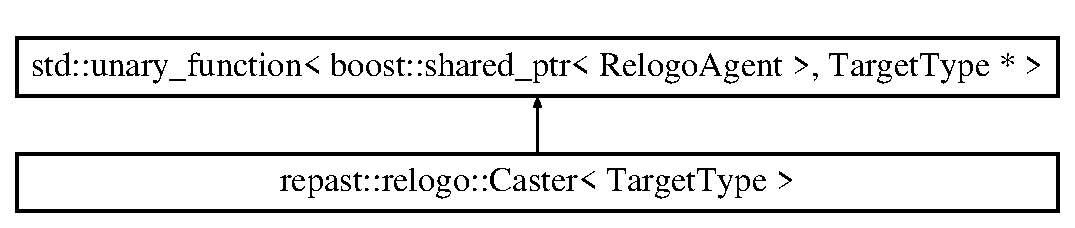
\includegraphics[height=2.000000cm]{structrepast_1_1relogo_1_1_caster}
\end{center}
\end{figure}
\subsection*{Public Member Functions}
\begin{DoxyCompactItemize}
\item 
\hypertarget{structrepast_1_1relogo_1_1_caster_ad472a8ecc1aa129b9c35728d44ce9940}{Target\-Type $\ast$ {\bfseries operator()} (boost\-::shared\-\_\-ptr$<$ \hyperlink{classrepast_1_1relogo_1_1_relogo_agent}{Relogo\-Agent} $>$ ptr) const }\label{structrepast_1_1relogo_1_1_caster_ad472a8ecc1aa129b9c35728d44ce9940}

\end{DoxyCompactItemize}


\subsection{Detailed Description}
\subsubsection*{template$<$typename Target\-Type$>$struct repast\-::relogo\-::\-Caster$<$ Target\-Type $>$}

Unary function used in the transform\-\_\-iterator that allows context iterators to return the agent maps values. 

The documentation for this struct was generated from the following file\-:\begin{DoxyCompactItemize}
\item 
/\-Users/murphy/work/\-Repast\-H\-P\-C\-\_\-\-G\-I\-T/repast.\-hpc/src/relogo/Observer.\-h\end{DoxyCompactItemize}

\hypertarget{structrepast_1_1relogo_1_1_caster2}{\section{repast\-:\-:relogo\-:\-:Caster2$<$ Target\-Type $>$ Struct Template Reference}
\label{structrepast_1_1relogo_1_1_caster2}\index{repast\-::relogo\-::\-Caster2$<$ Target\-Type $>$@{repast\-::relogo\-::\-Caster2$<$ Target\-Type $>$}}
}


Unary function used in the transform\-\_\-iterator that allows.  




{\ttfamily \#include $<$agent\-\_\-set\-\_\-functions.\-h$>$}

Inheritance diagram for repast\-:\-:relogo\-:\-:Caster2$<$ Target\-Type $>$\-:\begin{figure}[H]
\begin{center}
\leavevmode
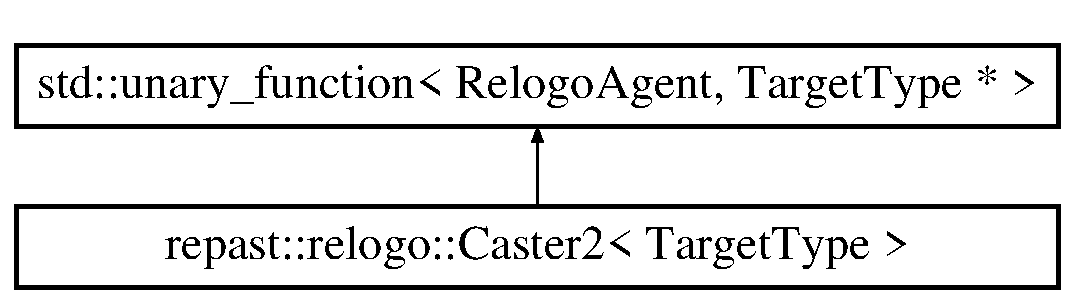
\includegraphics[height=2.000000cm]{structrepast_1_1relogo_1_1_caster2}
\end{center}
\end{figure}
\subsection*{Public Member Functions}
\begin{DoxyCompactItemize}
\item 
\hypertarget{structrepast_1_1relogo_1_1_caster2_ae50fa843df761aaba14938ce189ad995}{Target\-Type $\ast$ {\bfseries operator()} (const \hyperlink{classrepast_1_1relogo_1_1_relogo_agent}{Relogo\-Agent} $\ast$agent) const }\label{structrepast_1_1relogo_1_1_caster2_ae50fa843df761aaba14938ce189ad995}

\end{DoxyCompactItemize}


\subsection{Detailed Description}
\subsubsection*{template$<$typename Target\-Type$>$struct repast\-::relogo\-::\-Caster2$<$ Target\-Type $>$}

Unary function used in the transform\-\_\-iterator that allows. 

The documentation for this struct was generated from the following file\-:\begin{DoxyCompactItemize}
\item 
/\-Users/murphy/work/\-Repast\-H\-P\-C\-\_\-\-G\-I\-T/repast.\-hpc/src/relogo/agent\-\_\-set\-\_\-functions.\-h\end{DoxyCompactItemize}

\hypertarget{structrepast_1_1relogo_1_1_default_agent_creator}{\section{repast\-:\-:relogo\-:\-:Default\-Agent\-Creator$<$ Agent $>$ Struct Template Reference}
\label{structrepast_1_1relogo_1_1_default_agent_creator}\index{repast\-::relogo\-::\-Default\-Agent\-Creator$<$ Agent $>$@{repast\-::relogo\-::\-Default\-Agent\-Creator$<$ Agent $>$}}
}


operator() that creates an agent of type Agent.  




{\ttfamily \#include $<$creators.\-h$>$}

\subsection*{Public Member Functions}
\begin{DoxyCompactItemize}
\item 
\hypertarget{structrepast_1_1relogo_1_1_default_agent_creator_a56e7418784408bb366790b8ca7363e3a}{Agent $\ast$ {\bfseries operator()} (const repast\-::\-Agent\-Id \&id, \hyperlink{classrepast_1_1relogo_1_1_observer}{Observer} $\ast$obs)}\label{structrepast_1_1relogo_1_1_default_agent_creator_a56e7418784408bb366790b8ca7363e3a}

\end{DoxyCompactItemize}


\subsection{Detailed Description}
\subsubsection*{template$<$typename Agent$>$struct repast\-::relogo\-::\-Default\-Agent\-Creator$<$ Agent $>$}

operator() that creates an agent of type Agent. 

The type Agent must have a constructor that takes an Agent\-Id and pointer to an \hyperlink{classrepast_1_1relogo_1_1_observer}{Observer}. 

The documentation for this struct was generated from the following file\-:\begin{DoxyCompactItemize}
\item 
/\-Users/murphy/work/\-Repast\-H\-P\-C\-\_\-\-G\-I\-T/repast.\-hpc/src/relogo/creators.\-h\end{DoxyCompactItemize}

\hypertarget{structrepast_1_1relogo_1_1_default_link_creator}{\section{repast\-:\-:relogo\-:\-:Default\-Link\-Creator Struct Reference}
\label{structrepast_1_1relogo_1_1_default_link_creator}\index{repast\-::relogo\-::\-Default\-Link\-Creator@{repast\-::relogo\-::\-Default\-Link\-Creator}}
}


operator() that creates a \hyperlink{classrepast_1_1relogo_1_1_relogo_link}{Relogo\-Link} from a source and target Relogo\-Agents.  




{\ttfamily \#include $<$creators.\-h$>$}

\subsection*{Public Member Functions}
\begin{DoxyCompactItemize}
\item 
\hypertarget{structrepast_1_1relogo_1_1_default_link_creator_a1ad7ec806173027b48ab7095c442665e}{\hyperlink{classrepast_1_1relogo_1_1_relogo_link}{Relogo\-Link} $\ast$ {\bfseries operator()} (\hyperlink{classrepast_1_1relogo_1_1_relogo_agent}{Relogo\-Agent} $\ast$source, \hyperlink{classrepast_1_1relogo_1_1_relogo_agent}{Relogo\-Agent} $\ast$target)}\label{structrepast_1_1relogo_1_1_default_link_creator_a1ad7ec806173027b48ab7095c442665e}

\end{DoxyCompactItemize}


\subsection{Detailed Description}
operator() that creates a \hyperlink{classrepast_1_1relogo_1_1_relogo_link}{Relogo\-Link} from a source and target Relogo\-Agents. 

The documentation for this struct was generated from the following files\-:\begin{DoxyCompactItemize}
\item 
/\-Users/murphy/work/\-Repast\-H\-P\-C\-\_\-\-G\-I\-T/repast.\-hpc/src/relogo/creators.\-h\item 
/\-Users/murphy/work/\-Repast\-H\-P\-C\-\_\-\-G\-I\-T/repast.\-hpc/src/relogo/creators.\-cpp\end{DoxyCompactItemize}

\hypertarget{structrepast_1_1relogo_1_1_is_agent_type_no_dup}{\section{repast\-:\-:relogo\-:\-:Is\-Agent\-Type\-No\-Dup$<$ T $>$ Struct Template Reference}
\label{structrepast_1_1relogo_1_1_is_agent_type_no_dup}\index{repast\-::relogo\-::\-Is\-Agent\-Type\-No\-Dup$<$ T $>$@{repast\-::relogo\-::\-Is\-Agent\-Type\-No\-Dup$<$ T $>$}}
}


Used to filter by agent type but ensure that only the first encountered instance of agent is considered.  




{\ttfamily \#include $<$agent\-\_\-set\-\_\-functions.\-h$>$}

\subsection*{Public Member Functions}
\begin{DoxyCompactItemize}
\item 
\hypertarget{structrepast_1_1relogo_1_1_is_agent_type_no_dup_ae0f58dd650ad972fb5ac0948f1b74444}{{\bfseries Is\-Agent\-Type\-No\-Dup} (int type\-Id)}\label{structrepast_1_1relogo_1_1_is_agent_type_no_dup_ae0f58dd650ad972fb5ac0948f1b74444}

\item 
\hypertarget{structrepast_1_1relogo_1_1_is_agent_type_no_dup_a08dd36ccec0bbd029b12a3436b2907d1}{bool {\bfseries operator()} (const T $\ast$agent)}\label{structrepast_1_1relogo_1_1_is_agent_type_no_dup_a08dd36ccec0bbd029b12a3436b2907d1}

\end{DoxyCompactItemize}
\subsection*{Public Attributes}
\begin{DoxyCompactItemize}
\item 
\hypertarget{structrepast_1_1relogo_1_1_is_agent_type_no_dup_a78e50c14dc80ced45d0b166145cf4347}{Is\-Agent\-Type$<$ T $>$ {\bfseries is\-Agent\-Type}}\label{structrepast_1_1relogo_1_1_is_agent_type_no_dup_a78e50c14dc80ced45d0b166145cf4347}

\item 
\hypertarget{structrepast_1_1relogo_1_1_is_agent_type_no_dup_ac2fbe23e714eb452a9db119a6d4db5f1}{boost\-::unordered\-\_\-set$<$ Agent\-Id, \\*
Hash\-Id $>$ {\bfseries set}}\label{structrepast_1_1relogo_1_1_is_agent_type_no_dup_ac2fbe23e714eb452a9db119a6d4db5f1}

\end{DoxyCompactItemize}


\subsection{Detailed Description}
\subsubsection*{template$<$typename T$>$struct repast\-::relogo\-::\-Is\-Agent\-Type\-No\-Dup$<$ T $>$}

Used to filter by agent type but ensure that only the first encountered instance of agent is considered. 

The documentation for this struct was generated from the following file\-:\begin{DoxyCompactItemize}
\item 
/\-Users/murphy/work/\-Repast\-H\-P\-C\-\_\-\-G\-I\-T/repast.\-hpc/src/relogo/agent\-\_\-set\-\_\-functions.\-h\end{DoxyCompactItemize}

\hypertarget{classrepast_1_1relogo_1_1_observer}{\section{repast\-:\-:relogo\-:\-:Observer Class Reference}
\label{classrepast_1_1relogo_1_1_observer}\index{repast\-::relogo\-::\-Observer@{repast\-::relogo\-::\-Observer}}
}


Implementation of a logo \hyperlink{classrepast_1_1relogo_1_1_observer}{Observer}.  




{\ttfamily \#include $<$Observer.\-h$>$}

\subsection*{Public Member Functions}
\begin{DoxyCompactItemize}
\item 
void \hyperlink{classrepast_1_1relogo_1_1_observer_a08d634c4dde933cd0a690271e7b2edd6}{add\-Data\-Set} (repast\-::\-Data\-Set $\ast$data\-Set)
\begin{DoxyCompactList}\small\item\em Adds a dataset to this \hyperlink{classrepast_1_1relogo_1_1_observer}{Observer}. \end{DoxyCompactList}\item 
\hypertarget{classrepast_1_1relogo_1_1_observer_abcf29ed2775f06aa3e77d3140723d4ce}{void \hyperlink{classrepast_1_1relogo_1_1_observer_abcf29ed2775f06aa3e77d3140723d4ce}{data\-Set\-Close} ()}\label{classrepast_1_1relogo_1_1_observer_abcf29ed2775f06aa3e77d3140723d4ce}

\begin{DoxyCompactList}\small\item\em Non A\-P\-I method for closing all the datasets at the end of a sim runs. \end{DoxyCompactList}\item 
virtual void \hyperlink{classrepast_1_1relogo_1_1_observer_a4ab373d9fd531a50e788c5a6bac04002}{go} ()=0
\begin{DoxyCompactList}\small\item\em Called every tick of the simulation. \end{DoxyCompactList}\item 
virtual void \hyperlink{classrepast_1_1relogo_1_1_observer_a2780109d873c73115d44cddf8f138ef3}{setup} (Properties \&props)
\begin{DoxyCompactList}\small\item\em Classes that extend this should include model initialization here. \end{DoxyCompactList}\item 
void \hyperlink{classrepast_1_1relogo_1_1_observer_aa84ed23a631c997aaf5942eb22becfa5}{\-\_\-setup} (Properties \&props)
\begin{DoxyCompactList}\small\item\em Performs internal Relogo initialization. \end{DoxyCompactList}\item 
int \hyperlink{classrepast_1_1relogo_1_1_observer_a4b6cf502f73063c0d99af21e7a3eab50}{min\-Pxcor} () const 
\begin{DoxyCompactList}\small\item\em Gets the minimum x coordinate of the patches managed by this \hyperlink{classrepast_1_1relogo_1_1_observer}{Observer}. \end{DoxyCompactList}\item 
int \hyperlink{classrepast_1_1relogo_1_1_observer_a8b4a2f3c5b662a20caf690baa389be05}{min\-Pycor} () const 
\begin{DoxyCompactList}\small\item\em Gets the minimum y coordinate of the patches managed by this \hyperlink{classrepast_1_1relogo_1_1_observer}{Observer}. \end{DoxyCompactList}\item 
int \hyperlink{classrepast_1_1relogo_1_1_observer_a02da6b9980c4a06926e024234c708f85}{max\-Pxcor} () const 
\begin{DoxyCompactList}\small\item\em Gets the maximum x coordinate of the patches managed by this \hyperlink{classrepast_1_1relogo_1_1_observer}{Observer}. \end{DoxyCompactList}\item 
int \hyperlink{classrepast_1_1relogo_1_1_observer_a7435b47c62c790d656092fce3ce1647e}{max\-Pycor} () const 
\begin{DoxyCompactList}\small\item\em Gets the maximum y coordinate of the patches managed by this \hyperlink{classrepast_1_1relogo_1_1_observer}{Observer}. \end{DoxyCompactList}\item 
int \hyperlink{classrepast_1_1relogo_1_1_observer_a8a46f049d939c640f0e4094c17145dfd}{random\-Pxcor} ()
\begin{DoxyCompactList}\small\item\em Gets a random x coodinate of the patches managed by this \hyperlink{classrepast_1_1relogo_1_1_observer}{Observer}. \end{DoxyCompactList}\item 
int \hyperlink{classrepast_1_1relogo_1_1_observer_acf3115c0cd3cbd2f2b9d979ff166daa7}{random\-Pycor} ()
\begin{DoxyCompactList}\small\item\em Gets a random y coodinate of the patches managed by this \hyperlink{classrepast_1_1relogo_1_1_observer}{Observer}. \end{DoxyCompactList}\item 
double \hyperlink{classrepast_1_1relogo_1_1_observer_a0cb7be571b2750313e6678ce01b97a2c}{random\-Xcor} ()
\begin{DoxyCompactList}\small\item\em Gets a random x coodinate of the turtles managed by this \hyperlink{classrepast_1_1relogo_1_1_observer}{Observer}. \end{DoxyCompactList}\item 
double \hyperlink{classrepast_1_1relogo_1_1_observer_aba7a10326c6c8fe6e9de52ab073981e0}{random\-Ycor} ()
\begin{DoxyCompactList}\small\item\em Gets a random y coodinate of the turtles managed by this \hyperlink{classrepast_1_1relogo_1_1_observer}{Observer}. \end{DoxyCompactList}\item 
\hypertarget{classrepast_1_1relogo_1_1_observer_a67845540835cd3976a12adea78ede7b4}{bool {\bfseries space\-Pt\-To\-Grid\-Pt} (std\-::vector$<$ double $>$ \&space\-Pt, std\-::vector$<$ int $>$ \&grid\-Pt)}\label{classrepast_1_1relogo_1_1_observer_a67845540835cd3976a12adea78ede7b4}

\item 
{\footnotesize template$<$typename Agent\-Type $>$ }\\Agent\-Type $\ast$ \hyperlink{classrepast_1_1relogo_1_1_observer_ae9bccf456c22ebdc3faf71ca1ebc9931}{hatch} (\hyperlink{classrepast_1_1relogo_1_1_relogo_agent}{Relogo\-Agent} $\ast$parent)
\begin{DoxyCompactList}\small\item\em Hatchs an agent of the specified type. \end{DoxyCompactList}\item 
{\footnotesize template$<$typename Agent\-Type , typename Factory\-Functor $>$ }\\Agent\-Type $\ast$ \hyperlink{classrepast_1_1relogo_1_1_observer_afece369146d9b5c0f4ec1a46e8d570e1}{hatch} (\hyperlink{classrepast_1_1relogo_1_1_relogo_agent}{Relogo\-Agent} $\ast$parent, Factory\-Functor agent\-Creator)
\begin{DoxyCompactList}\small\item\em Hatchs an agent of the specified type. \end{DoxyCompactList}\item 
{\footnotesize template$<$typename Agent\-Type $>$ }\\Agent\-Type $\ast$ \hyperlink{classrepast_1_1relogo_1_1_observer_a00d27f676b62f1c0dbd5d30e842983ca}{who} (const Agent\-Id \&id)
\begin{DoxyCompactList}\small\item\em Gets the agent with the specified id. \end{DoxyCompactList}\item 
{\footnotesize template$<$typename Agent\-Type $>$ }\\int \hyperlink{classrepast_1_1relogo_1_1_observer_adf2bea53506dfc407f5c72ad506f634f}{create} (size\-\_\-t count)
\begin{DoxyCompactList}\small\item\em Create count number of agents of the specified type. \end{DoxyCompactList}\item 
{\footnotesize template$<$typename Agent\-Type , typename Factory\-Functor $>$ }\\int \hyperlink{classrepast_1_1relogo_1_1_observer_a560cc8f342873668d6ffedd980bbd623}{create} (size\-\_\-t count, Factory\-Functor agent\-Creator)
\begin{DoxyCompactList}\small\item\em Create count number of agents of the specified type, using the specified Factory\-Functor. \end{DoxyCompactList}\item 
\hypertarget{classrepast_1_1relogo_1_1_observer_a4f788359649fb91f08284628aa86e23d}{void \hyperlink{classrepast_1_1relogo_1_1_observer_a4f788359649fb91f08284628aa86e23d}{remove\-Agent} (const Agent\-Id \&id)}\label{classrepast_1_1relogo_1_1_observer_a4f788359649fb91f08284628aa86e23d}

\begin{DoxyCompactList}\small\item\em Removes the specified turtle from the world. \end{DoxyCompactList}\item 
{\footnotesize template$<$typename Agent\-Type $>$ }\\\hyperlink{classrepast_1_1relogo_1_1_agent_set}{Agent\-Set}$<$ Agent\-Type $>$ \hyperlink{classrepast_1_1relogo_1_1_observer_adc2973bf611da5b3150241767ea0aaf4}{get} ()
\begin{DoxyCompactList}\small\item\em Gets all of the agents of the templated type and returns them in an \hyperlink{classrepast_1_1relogo_1_1_agent_set}{Agent\-Set}. \end{DoxyCompactList}\item 
\hypertarget{classrepast_1_1relogo_1_1_observer_a801236adc73230ae18d3f52c88462c16}{\hyperlink{classrepast_1_1relogo_1_1_agent_set}{Agent\-Set}$<$ \hyperlink{classrepast_1_1relogo_1_1_turtle}{Turtle} $>$ \hyperlink{classrepast_1_1relogo_1_1_observer_a801236adc73230ae18d3f52c88462c16}{turtles} ()}\label{classrepast_1_1relogo_1_1_observer_a801236adc73230ae18d3f52c88462c16}

\begin{DoxyCompactList}\small\item\em Gets all the turtles in this world and return them in the \hyperlink{classrepast_1_1relogo_1_1_agent_set}{Agent\-Set}. \end{DoxyCompactList}\item 
void \hyperlink{classrepast_1_1relogo_1_1_observer_aecb694175ac25b641ab39fdf66a1d865}{get} (\hyperlink{classrepast_1_1relogo_1_1_agent_set}{Agent\-Set}$<$ \hyperlink{classrepast_1_1relogo_1_1_turtle}{Turtle} $>$ \&\hyperlink{classrepast_1_1relogo_1_1_observer_a801236adc73230ae18d3f52c88462c16}{turtles})
\begin{DoxyCompactList}\small\item\em Gets all the turtles in this world and put them into the specified \hyperlink{classrepast_1_1relogo_1_1_agent_set}{Agent\-Set}. \end{DoxyCompactList}\item 
{\footnotesize template$<$typename Agent\-Type $>$ }\\void \hyperlink{classrepast_1_1relogo_1_1_observer_a895df31674a579f8eb506cf76cfc1dba}{get} (\hyperlink{classrepast_1_1relogo_1_1_agent_set}{Agent\-Set}$<$ Agent\-Type $>$ \&agent\-Set)
\begin{DoxyCompactList}\small\item\em Gets all of the agents of the templated type and puts them into the agent\-Set. \end{DoxyCompactList}\item 
{\footnotesize template$<$typename Agent\-Type $>$ }\\Agent\-Type $\ast$ \hyperlink{classrepast_1_1relogo_1_1_observer_a7251d8ec999c10df60cbe55b45f84e16}{get} (const Agent\-Id \&id)
\begin{DoxyCompactList}\small\item\em Gets the turtle with the specified id or 0 if no such turtle is found. \end{DoxyCompactList}\item 
{\footnotesize template$<$typename Agent\-Type $>$ }\\\hyperlink{classrepast_1_1relogo_1_1_agent_set}{Agent\-Set}$<$ Agent\-Type $>$ \hyperlink{classrepast_1_1relogo_1_1_observer_a8d1157c42f9ae822860e9865cb871741}{turtles\-At} (int x, int y)
\begin{DoxyCompactList}\small\item\em Gets all of the agents of the templated type at the specified patch location. \end{DoxyCompactList}\item 
{\footnotesize template$<$typename Agent\-Type $>$ }\\void \hyperlink{classrepast_1_1relogo_1_1_observer_aa35e9afb1ecc83b3bb5c2b62c1059cdc}{turtles\-At} (int x, int y, \hyperlink{classrepast_1_1relogo_1_1_agent_set}{Agent\-Set}$<$ Agent\-Type $>$ \&set)
\begin{DoxyCompactList}\small\item\em Gets all of the agents of the templated type at the specified patch location and puts them in the specified set. \end{DoxyCompactList}\item 
int \hyperlink{classrepast_1_1relogo_1_1_observer_aca1427918732c400436240998ba1739f}{rank} () const 
\begin{DoxyCompactList}\small\item\em Gets the process rank of this \hyperlink{classrepast_1_1relogo_1_1_observer}{Observer}. \end{DoxyCompactList}\item 
const Relogo\-Grid\-Type $\ast$ \hyperlink{classrepast_1_1relogo_1_1_observer_a11b3edc4275730a56775fc8f275b47c7}{grid} ()
\begin{DoxyCompactList}\small\item\em Gets the grid managed by this \hyperlink{classrepast_1_1relogo_1_1_observer}{Observer}. \end{DoxyCompactList}\item 
const Relogo\-Space\-Type $\ast$ \hyperlink{classrepast_1_1relogo_1_1_observer_aea3636a7f63319553eee9e0b09d2523c}{space} ()
\begin{DoxyCompactList}\small\item\em Gets the space managed by this \hyperlink{classrepast_1_1relogo_1_1_observer}{Observer}. \end{DoxyCompactList}\item 
void \hyperlink{classrepast_1_1relogo_1_1_observer_aa6a58226752ace6c89cff6cdd546806b}{create\-Link} (\hyperlink{classrepast_1_1relogo_1_1_relogo_agent}{Relogo\-Agent} $\ast$source, \hyperlink{classrepast_1_1relogo_1_1_relogo_agent}{Relogo\-Agent} $\ast$target, const std\-::string \&network\-Name)
\begin{DoxyCompactList}\small\item\em Creates a link between the source and target agents in the named network. \end{DoxyCompactList}\item 
{\footnotesize template$<$typename Link\-Creator $>$ }\\void \hyperlink{classrepast_1_1relogo_1_1_observer_a82c935b25859fb94e8010e25ee880854}{create\-Link} (\hyperlink{classrepast_1_1relogo_1_1_relogo_agent}{Relogo\-Agent} $\ast$source, \hyperlink{classrepast_1_1relogo_1_1_relogo_agent}{Relogo\-Agent} $\ast$target, const std\-::string \&network\-Name, Link\-Creator \&creator)
\begin{DoxyCompactList}\small\item\em Creates a link between the source and target agents in the named network, using the specified Link\-Creator. \end{DoxyCompactList}\item 
boost\-::shared\-\_\-ptr$<$ \hyperlink{classrepast_1_1relogo_1_1_relogo_link}{Relogo\-Link} $>$ \hyperlink{classrepast_1_1relogo_1_1_observer_a26e12713f282594d49b31919de373f25}{link} (\hyperlink{classrepast_1_1relogo_1_1_relogo_agent}{Relogo\-Agent} $\ast$source, \hyperlink{classrepast_1_1relogo_1_1_relogo_agent}{Relogo\-Agent} $\ast$target, const std\-::string \&network\-Name)
\begin{DoxyCompactList}\small\item\em Gets the link, if any, between the source and target agents in the named network. \end{DoxyCompactList}\item 
{\footnotesize template$<$typename Agent\-Type $>$ }\\void \hyperlink{classrepast_1_1relogo_1_1_observer_a01f927604bdd537d650596604703d09c}{predecessors} (\hyperlink{classrepast_1_1relogo_1_1_relogo_agent}{Relogo\-Agent} $\ast$agent, const std\-::string \&network\-Name, \hyperlink{classrepast_1_1relogo_1_1_agent_set}{Agent\-Set}$<$ Agent\-Type $>$ \&out)
\begin{DoxyCompactList}\small\item\em Gets the network predecessors of the specified agent in the specified network and puts the result into out. \end{DoxyCompactList}\item 
{\footnotesize template$<$typename Agent\-Type $>$ }\\void \hyperlink{classrepast_1_1relogo_1_1_observer_a225bb07be2ba509b88746bff2e6d8745}{successors} (\hyperlink{classrepast_1_1relogo_1_1_relogo_agent}{Relogo\-Agent} $\ast$agent, const std\-::string \&network\-Name, \hyperlink{classrepast_1_1relogo_1_1_agent_set}{Agent\-Set}$<$ Agent\-Type $>$ \&out)
\begin{DoxyCompactList}\small\item\em Gets the network successors of the specified agent in the specified network and puts the result into out. \end{DoxyCompactList}\item 
{\footnotesize template$<$typename Patch\-Type $>$ }\\Patch\-Type $\ast$ \hyperlink{classrepast_1_1relogo_1_1_observer_a78c7ec8b81efadd6a3a1050ddf9043ce}{patch\-At} (int x, int y)
\begin{DoxyCompactList}\small\item\em Gets the patch at the specified coordinates. \end{DoxyCompactList}\item 
\hyperlink{classrepast_1_1relogo_1_1_patch}{Patch} $\ast$ \hyperlink{classrepast_1_1relogo_1_1_observer_ad573c6f1bd2d8c8047d025652a43100c}{patch\-At} (int x, int y)
\begin{DoxyCompactList}\small\item\em Gets the patch at the specified coordinates. \end{DoxyCompactList}\item 
\hyperlink{classrepast_1_1relogo_1_1_patch}{Patch} $\ast$ \hyperlink{classrepast_1_1relogo_1_1_observer_a94254d970a0e8f8409b1fa0aca0aab5b}{patch\-At} (Point$<$ double $>$ location, double dx, double dy)
\begin{DoxyCompactList}\small\item\em Gets the patch at the delta from the specified location or 0 if the resulting location is outside the world. \end{DoxyCompactList}\item 
\hyperlink{classrepast_1_1relogo_1_1_patch}{Patch} $\ast$ \hyperlink{classrepast_1_1relogo_1_1_observer_acb1163537fb7f53ccb6cf99d1cfdff47}{patch\-At\-Offset} (Point$<$ double $>$ location, double heading, double distance)
\begin{DoxyCompactList}\small\item\em Gets the patch at the heading/distance offset from the specified location or 0 if the resulting location is outside the world. \end{DoxyCompactList}\item 
{\footnotesize template$<$typename Patch\-Type $>$ }\\\hyperlink{classrepast_1_1relogo_1_1_agent_set}{Agent\-Set}$<$ Patch\-Type $>$ \hyperlink{classrepast_1_1relogo_1_1_observer_ad68866a2584551d27c9bb6c53aca5f20}{patches} ()
\begin{DoxyCompactList}\small\item\em Gets an agent set of the all the patches. \end{DoxyCompactList}\item 
{\footnotesize template$<$typename Patch\-Type $>$ }\\void \hyperlink{classrepast_1_1relogo_1_1_observer_a2384690c4e773727acdccaa7fc314bcd}{patches} (\hyperlink{classrepast_1_1relogo_1_1_agent_set}{Agent\-Set}$<$ Patch\-Type $>$ \&set)
\begin{DoxyCompactList}\small\item\em Gets all the patches and places them in the specified set. \end{DoxyCompactList}\item 
{\footnotesize template$<$typename Turtle\-Type $>$ }\\void \hyperlink{classrepast_1_1relogo_1_1_observer_aad4c5fbcf929481f361cca41c4b432ec}{turtles\-On} (\hyperlink{classrepast_1_1relogo_1_1_agent_set}{Agent\-Set}$<$ \hyperlink{classrepast_1_1relogo_1_1_relogo_agent}{Relogo\-Agent} $>$ \&agent\-Set, \hyperlink{classrepast_1_1relogo_1_1_agent_set}{Agent\-Set}$<$ Turtle\-Type $>$ \&out)
\begin{DoxyCompactList}\small\item\em Gets all the turtles that are on any patches contained in the agent\-Set or on the patches where any turtles in the agent\-Set are standing. \end{DoxyCompactList}\item 
{\footnotesize template$<$typename Turtle\-Type $>$ }\\void \hyperlink{classrepast_1_1relogo_1_1_observer_aedb92a41bdaafe4a179f2b4a027e7929}{turtles\-On} (const \hyperlink{classrepast_1_1relogo_1_1_relogo_agent}{Relogo\-Agent} $\ast$agent, \hyperlink{classrepast_1_1relogo_1_1_agent_set}{Agent\-Set}$<$ Turtle\-Type $>$ \&out)
\begin{DoxyCompactList}\small\item\em Gets all the turtles that are on the patch if the agent is a patch, otherwise get all the agents on the patch where the agent is standing. \end{DoxyCompactList}\item 
{\footnotesize template$<$typename Agent\-Type $>$ }\\void \hyperlink{classrepast_1_1relogo_1_1_observer_a1e832a3c9c59198c105e39e4820b4be3}{in\-Radius} (const Point$<$ double $>$ \&center, \hyperlink{classrepast_1_1relogo_1_1_agent_set}{Agent\-Set}$<$ \hyperlink{classrepast_1_1relogo_1_1_relogo_agent}{Relogo\-Agent} $>$ \&in\-Set, double radius, \hyperlink{classrepast_1_1relogo_1_1_agent_set}{Agent\-Set}$<$ Agent\-Type $>$ \&out\-Set)
\begin{DoxyCompactList}\small\item\em Puts all the agents in the in\-Set that are of the specified type and within the specified radius from the specified center into the out\-Set. \end{DoxyCompactList}\item 
{\footnotesize template$<$typename Turtle\-Content , typename Provider , typename Updater , typename Agent\-Creator $>$ }\\void \hyperlink{classrepast_1_1relogo_1_1_observer_a966b0c9fac6e6d4e3e21f74ac3b955b6}{synchronize\-Turtle\-Status} (Provider \&provider, Updater \&updater, Agent\-Creator \&creator, Repast\-Process\-::\-E\-X\-C\-H\-A\-N\-G\-E\-\_\-\-P\-A\-T\-T\-E\-R\-N exchange\-Pattern=Repast\-Process\-::\-P\-O\-L\-L)
\begin{DoxyCompactList}\small\item\em Synchronizes the status (moved or died) of all turtles across processes. \end{DoxyCompactList}\item 
{\footnotesize template$<$typename Turtle\-Content , typename Provider , typename Updater $>$ }\\void \hyperlink{classrepast_1_1relogo_1_1_observer_a4db8efa2a511050a5432c185816d3cec}{synchronize\-Turtle\-States} (Provider \&provider, Updater \&updater)
\begin{DoxyCompactList}\small\item\em Synchronizes the state of any Turtles that are shared across processes. \end{DoxyCompactList}\item 
\hypertarget{classrepast_1_1relogo_1_1_observer_a0268b843eec648ada141c031f6a13621}{{\footnotesize template$<$typename Turtle\-Content , typename Provider , typename Updater , typename Agent\-Creator $>$ }\\void {\bfseries synchronize} (Provider \&provider, Updater \&updater, Agent\-Creator \&creator, Repast\-Process\-::\-E\-X\-C\-H\-A\-N\-G\-E\-\_\-\-P\-A\-T\-T\-E\-R\-N exchange\-Pattern=Repast\-Process\-::\-P\-O\-L\-L)}\label{classrepast_1_1relogo_1_1_observer_a0268b843eec648ada141c031f6a13621}

\item 
\hypertarget{classrepast_1_1relogo_1_1_observer_aa7cb67c53a3a3b5012494bb45f0c6b40}{{\footnotesize template$<$typename Agent $>$ }\\\hyperlink{classrepast_1_1relogo_1_1_agent_set}{Agent\-Set}$<$ Agent $>$ {\bfseries get} ()}\label{classrepast_1_1relogo_1_1_observer_aa7cb67c53a3a3b5012494bb45f0c6b40}

\end{DoxyCompactItemize}
\subsection*{Protected Types}
\begin{DoxyCompactItemize}
\item 
\hypertarget{classrepast_1_1relogo_1_1_observer_a217887f3aa32a6ede5e1e501d68cfe76}{typedef Shared\-Network\\*
$<$ \hyperlink{classrepast_1_1relogo_1_1_relogo_agent}{Relogo\-Agent}, \hyperlink{classrepast_1_1relogo_1_1_relogo_link}{Relogo\-Link}, \\*
Repast\-Edge\-Content$<$ \hyperlink{classrepast_1_1relogo_1_1_relogo_agent}{Relogo\-Agent} $>$\\*
, Repast\-Edge\-Content\-Manager\\*
$<$ \hyperlink{classrepast_1_1relogo_1_1_relogo_agent}{Relogo\-Agent} $>$ $>$ {\bfseries Network\-Type}}\label{classrepast_1_1relogo_1_1_observer_a217887f3aa32a6ede5e1e501d68cfe76}

\end{DoxyCompactItemize}
\subsection*{Protected Member Functions}
\begin{DoxyCompactItemize}
\item 
\hypertarget{classrepast_1_1relogo_1_1_observer_a9a6da36977fc44e0364be1d7032055ca}{Network\-Type $\ast$ {\bfseries find\-Network} (const std\-::string \&name)}\label{classrepast_1_1relogo_1_1_observer_a9a6da36977fc44e0364be1d7032055ca}

\end{DoxyCompactItemize}
\subsection*{Protected Attributes}
\begin{DoxyCompactItemize}
\item 
\hypertarget{classrepast_1_1relogo_1_1_observer_a77aae0a56dedd99a7ae481c74407e8d2}{Properties {\bfseries \-\_\-props}}\label{classrepast_1_1relogo_1_1_observer_a77aae0a56dedd99a7ae481c74407e8d2}

\item 
\hypertarget{classrepast_1_1relogo_1_1_observer_a886b32011faa0ed43e084908d80d995b}{int {\bfseries \-\_\-rank}}\label{classrepast_1_1relogo_1_1_observer_a886b32011faa0ed43e084908d80d995b}

\item 
\hypertarget{classrepast_1_1relogo_1_1_observer_a242cab3ecef167edeed2f8598fd7220d}{Grid\-Dimensions {\bfseries local\-Bounds}}\label{classrepast_1_1relogo_1_1_observer_a242cab3ecef167edeed2f8598fd7220d}

\item 
\hypertarget{classrepast_1_1relogo_1_1_observer_a69c5a7ee964212debd1b2a60f75ba847}{repast\-::\-Shared\-Context\\*
$<$ \hyperlink{classrepast_1_1relogo_1_1_relogo_agent}{Relogo\-Agent} $>$ {\bfseries context}}\label{classrepast_1_1relogo_1_1_observer_a69c5a7ee964212debd1b2a60f75ba847}

\item 
\hypertarget{classrepast_1_1relogo_1_1_observer_aaf7ab7bd044b24b5903e8c8fd65feefc}{std\-::vector$<$ repast\-::\-Data\-Set $\ast$ $>$ {\bfseries data\-Sets}}\label{classrepast_1_1relogo_1_1_observer_aaf7ab7bd044b24b5903e8c8fd65feefc}

\end{DoxyCompactItemize}
\subsection*{Friends}
\begin{DoxyCompactItemize}
\item 
\hypertarget{classrepast_1_1relogo_1_1_observer_a8d256944f28ec0cd654da58d4dcff11c}{class {\bfseries World\-Creator}}\label{classrepast_1_1relogo_1_1_observer_a8d256944f28ec0cd654da58d4dcff11c}

\end{DoxyCompactItemize}


\subsection{Detailed Description}
Implementation of a logo \hyperlink{classrepast_1_1relogo_1_1_observer}{Observer}. 

\subsection{Member Function Documentation}
\hypertarget{classrepast_1_1relogo_1_1_observer_aa84ed23a631c997aaf5942eb22becfa5}{\index{repast\-::relogo\-::\-Observer@{repast\-::relogo\-::\-Observer}!\-\_\-setup@{\-\_\-setup}}
\index{\-\_\-setup@{\-\_\-setup}!repast::relogo::Observer@{repast\-::relogo\-::\-Observer}}
\subsubsection[{\-\_\-setup}]{\setlength{\rightskip}{0pt plus 5cm}void repast\-::relogo\-::\-Observer\-::\-\_\-setup (
\begin{DoxyParamCaption}
\item[{Properties \&}]{props}
\end{DoxyParamCaption}
)}}\label{classrepast_1_1relogo_1_1_observer_aa84ed23a631c997aaf5942eb22becfa5}


Performs internal Relogo initialization. 


\begin{DoxyParams}{Parameters}
{\em props} & Properties collection that can be used to drive initialization \\
\hline
\end{DoxyParams}
\hypertarget{classrepast_1_1relogo_1_1_observer_a08d634c4dde933cd0a690271e7b2edd6}{\index{repast\-::relogo\-::\-Observer@{repast\-::relogo\-::\-Observer}!add\-Data\-Set@{add\-Data\-Set}}
\index{add\-Data\-Set@{add\-Data\-Set}!repast::relogo::Observer@{repast\-::relogo\-::\-Observer}}
\subsubsection[{add\-Data\-Set}]{\setlength{\rightskip}{0pt plus 5cm}void repast\-::relogo\-::\-Observer\-::add\-Data\-Set (
\begin{DoxyParamCaption}
\item[{repast\-::\-Data\-Set $\ast$}]{data\-Set}
\end{DoxyParamCaption}
)}}\label{classrepast_1_1relogo_1_1_observer_a08d634c4dde933cd0a690271e7b2edd6}


Adds a dataset to this \hyperlink{classrepast_1_1relogo_1_1_observer}{Observer}. 

This observer will schedule the dataset for recording and writing, and properly destroy the dataset.


\begin{DoxyParams}{Parameters}
{\em data\-Set} & the data set to add \\
\hline
\end{DoxyParams}
\hypertarget{classrepast_1_1relogo_1_1_observer_adf2bea53506dfc407f5c72ad506f634f}{\index{repast\-::relogo\-::\-Observer@{repast\-::relogo\-::\-Observer}!create@{create}}
\index{create@{create}!repast::relogo::Observer@{repast\-::relogo\-::\-Observer}}
\subsubsection[{create}]{\setlength{\rightskip}{0pt plus 5cm}template$<$typename Agent\-Type $>$ int repast\-::relogo\-::\-Observer\-::create (
\begin{DoxyParamCaption}
\item[{size\-\_\-t}]{count}
\end{DoxyParamCaption}
)}}\label{classrepast_1_1relogo_1_1_observer_adf2bea53506dfc407f5c72ad506f634f}


Create count number of agents of the specified type. 


\begin{DoxyParams}{Parameters}
{\em count} & the number of agents to create \\
\hline
\end{DoxyParams}

\begin{DoxyTemplParams}{Template Parameters}
{\em Agent\-Type} & the type of agents to create. This must be a \hyperlink{classrepast_1_1relogo_1_1_turtle}{Turtle} or a class that extends \hyperlink{classrepast_1_1relogo_1_1_turtle}{Turtle}. It must have a constructor that takes an Agent\-Id and a pointer to this \hyperlink{classrepast_1_1relogo_1_1_observer}{Observer}.\\
\hline
\end{DoxyTemplParams}
\begin{DoxyReturn}{Returns}
the integer type id for agents of this type. 
\end{DoxyReturn}
\hypertarget{classrepast_1_1relogo_1_1_observer_a560cc8f342873668d6ffedd980bbd623}{\index{repast\-::relogo\-::\-Observer@{repast\-::relogo\-::\-Observer}!create@{create}}
\index{create@{create}!repast::relogo::Observer@{repast\-::relogo\-::\-Observer}}
\subsubsection[{create}]{\setlength{\rightskip}{0pt plus 5cm}template$<$typename Agent\-Type , typename Factory\-Functor $>$ int repast\-::relogo\-::\-Observer\-::create (
\begin{DoxyParamCaption}
\item[{size\-\_\-t}]{count, }
\item[{Factory\-Functor}]{agent\-Creator}
\end{DoxyParamCaption}
)}}\label{classrepast_1_1relogo_1_1_observer_a560cc8f342873668d6ffedd980bbd623}


Create count number of agents of the specified type, using the specified Factory\-Functor. 


\begin{DoxyParams}{Parameters}
{\em count} & the number of agents to create \\
\hline
{\em agent\-Creator} & a Factory\-Functor used to create the agents\\
\hline
\end{DoxyParams}

\begin{DoxyTemplParams}{Template Parameters}
{\em Agent\-Type} & the type of agent to create. This must either be a \hyperlink{classrepast_1_1relogo_1_1_turtle}{Turtle} or extend \hyperlink{classrepast_1_1relogo_1_1_turtle}{Turtle}. \\
\hline
{\em Factory\-Functor} & a functor or function with the following signature Agent\-Type$\ast$ (Agent\-Id id, Observer$\ast$ obs).\\
\hline
\end{DoxyTemplParams}
\begin{DoxyReturn}{Returns}
an the integer id for agents of this type 
\end{DoxyReturn}
\hypertarget{classrepast_1_1relogo_1_1_observer_aa6a58226752ace6c89cff6cdd546806b}{\index{repast\-::relogo\-::\-Observer@{repast\-::relogo\-::\-Observer}!create\-Link@{create\-Link}}
\index{create\-Link@{create\-Link}!repast::relogo::Observer@{repast\-::relogo\-::\-Observer}}
\subsubsection[{create\-Link}]{\setlength{\rightskip}{0pt plus 5cm}void repast\-::relogo\-::\-Observer\-::create\-Link (
\begin{DoxyParamCaption}
\item[{{\bf Relogo\-Agent} $\ast$}]{source, }
\item[{{\bf Relogo\-Agent} $\ast$}]{target, }
\item[{const std\-::string \&}]{network\-Name}
\end{DoxyParamCaption}
)}}\label{classrepast_1_1relogo_1_1_observer_aa6a58226752ace6c89cff6cdd546806b}


Creates a link between the source and target agents in the named network. 


\begin{DoxyParams}{Parameters}
{\em source} & the source agent \\
\hline
{\em target} & the target agent \\
\hline
{\em network\-Name} & the name of the network to create the link in \\
\hline
\end{DoxyParams}
\hypertarget{classrepast_1_1relogo_1_1_observer_a82c935b25859fb94e8010e25ee880854}{\index{repast\-::relogo\-::\-Observer@{repast\-::relogo\-::\-Observer}!create\-Link@{create\-Link}}
\index{create\-Link@{create\-Link}!repast::relogo::Observer@{repast\-::relogo\-::\-Observer}}
\subsubsection[{create\-Link}]{\setlength{\rightskip}{0pt plus 5cm}template$<$typename Link\-Creator $>$ void repast\-::relogo\-::\-Observer\-::create\-Link (
\begin{DoxyParamCaption}
\item[{{\bf Relogo\-Agent} $\ast$}]{source, }
\item[{{\bf Relogo\-Agent} $\ast$}]{target, }
\item[{const std\-::string \&}]{network\-Name, }
\item[{Link\-Creator \&}]{creator}
\end{DoxyParamCaption}
)}}\label{classrepast_1_1relogo_1_1_observer_a82c935b25859fb94e8010e25ee880854}


Creates a link between the source and target agents in the named network, using the specified Link\-Creator. 


\begin{DoxyParams}{Parameters}
{\em source} & the source agent \\
\hline
{\em target} & the target agent \\
\hline
{\em network\-Name} & the name of the network to create the link in\\
\hline
\end{DoxyParams}

\begin{DoxyTemplParams}{Template Parameters}
{\em Link\-Creator} & an function or functor with the following signature Relogo\-Link$\ast$ (Turtle$\ast$ source, Turtle$\ast$ target) \\
\hline
\end{DoxyTemplParams}
\hypertarget{classrepast_1_1relogo_1_1_observer_adc2973bf611da5b3150241767ea0aaf4}{\index{repast\-::relogo\-::\-Observer@{repast\-::relogo\-::\-Observer}!get@{get}}
\index{get@{get}!repast::relogo::Observer@{repast\-::relogo\-::\-Observer}}
\subsubsection[{get}]{\setlength{\rightskip}{0pt plus 5cm}template$<$typename Agent\-Type $>$ {\bf Agent\-Set}$<$Agent\-Type$>$ repast\-::relogo\-::\-Observer\-::get (
\begin{DoxyParamCaption}
{}
\end{DoxyParamCaption}
)}}\label{classrepast_1_1relogo_1_1_observer_adc2973bf611da5b3150241767ea0aaf4}


Gets all of the agents of the templated type and returns them in an \hyperlink{classrepast_1_1relogo_1_1_agent_set}{Agent\-Set}. 


\begin{DoxyTemplParams}{Template Parameters}
{\em Agent\-Type} & the type of turtle agents to get \\
\hline
\end{DoxyTemplParams}
\begin{DoxyReturn}{Returns}
an agent set containing the agents 
\end{DoxyReturn}
\hypertarget{classrepast_1_1relogo_1_1_observer_aecb694175ac25b641ab39fdf66a1d865}{\index{repast\-::relogo\-::\-Observer@{repast\-::relogo\-::\-Observer}!get@{get}}
\index{get@{get}!repast::relogo::Observer@{repast\-::relogo\-::\-Observer}}
\subsubsection[{get}]{\setlength{\rightskip}{0pt plus 5cm}void repast\-::relogo\-::\-Observer\-::get (
\begin{DoxyParamCaption}
\item[{{\bf Agent\-Set}$<$ {\bf Turtle} $>$ \&}]{turtles}
\end{DoxyParamCaption}
)}}\label{classrepast_1_1relogo_1_1_observer_aecb694175ac25b641ab39fdf66a1d865}


Gets all the turtles in this world and put them into the specified \hyperlink{classrepast_1_1relogo_1_1_agent_set}{Agent\-Set}. 


\begin{DoxyParams}{Parameters}
{\em turtles} & the \hyperlink{classrepast_1_1relogo_1_1_agent_set}{Agent\-Set} to put the turtles in \\
\hline
\end{DoxyParams}
\hypertarget{classrepast_1_1relogo_1_1_observer_a895df31674a579f8eb506cf76cfc1dba}{\index{repast\-::relogo\-::\-Observer@{repast\-::relogo\-::\-Observer}!get@{get}}
\index{get@{get}!repast::relogo::Observer@{repast\-::relogo\-::\-Observer}}
\subsubsection[{get}]{\setlength{\rightskip}{0pt plus 5cm}template$<$typename Agent\-Type $>$ void repast\-::relogo\-::\-Observer\-::get (
\begin{DoxyParamCaption}
\item[{{\bf Agent\-Set}$<$ Agent\-Type $>$ \&}]{agent\-Set}
\end{DoxyParamCaption}
)}}\label{classrepast_1_1relogo_1_1_observer_a895df31674a579f8eb506cf76cfc1dba}


Gets all of the agents of the templated type and puts them into the agent\-Set. 


\begin{DoxyParams}{Parameters}
{\em agent\-Set} & the \hyperlink{classrepast_1_1relogo_1_1_agent_set}{Agent\-Set} to put the found agents in\\
\hline
\end{DoxyParams}

\begin{DoxyTemplParams}{Template Parameters}
{\em Agent\-Type} & the type of turtle agents to get \\
\hline
\end{DoxyTemplParams}
\begin{DoxyReturn}{Returns}
an agent set containing the agents 
\end{DoxyReturn}
\hypertarget{classrepast_1_1relogo_1_1_observer_a7251d8ec999c10df60cbe55b45f84e16}{\index{repast\-::relogo\-::\-Observer@{repast\-::relogo\-::\-Observer}!get@{get}}
\index{get@{get}!repast::relogo::Observer@{repast\-::relogo\-::\-Observer}}
\subsubsection[{get}]{\setlength{\rightskip}{0pt plus 5cm}template$<$typename Agent\-Type $>$ Agent\-Type $\ast$ repast\-::relogo\-::\-Observer\-::get (
\begin{DoxyParamCaption}
\item[{const Agent\-Id \&}]{id}
\end{DoxyParamCaption}
)}}\label{classrepast_1_1relogo_1_1_observer_a7251d8ec999c10df60cbe55b45f84e16}


Gets the turtle with the specified id or 0 if no such turtle is found. 


\begin{DoxyTemplParams}{Template Parameters}
{\em Agent\-Type} & the type of the turtle to find \\
\hline
\end{DoxyTemplParams}
\begin{DoxyReturn}{Returns}
the turtle with the specified id, or 0. 
\end{DoxyReturn}
\hypertarget{classrepast_1_1relogo_1_1_observer_a4ab373d9fd531a50e788c5a6bac04002}{\index{repast\-::relogo\-::\-Observer@{repast\-::relogo\-::\-Observer}!go@{go}}
\index{go@{go}!repast::relogo::Observer@{repast\-::relogo\-::\-Observer}}
\subsubsection[{go}]{\setlength{\rightskip}{0pt plus 5cm}virtual void repast\-::relogo\-::\-Observer\-::go (
\begin{DoxyParamCaption}
{}
\end{DoxyParamCaption}
)\hspace{0.3cm}{\ttfamily [pure virtual]}}}\label{classrepast_1_1relogo_1_1_observer_a4ab373d9fd531a50e788c5a6bac04002}


Called every tick of the simulation. 

Implementations of this method will implement that actual simulation behavior. \hypertarget{classrepast_1_1relogo_1_1_observer_a11b3edc4275730a56775fc8f275b47c7}{\index{repast\-::relogo\-::\-Observer@{repast\-::relogo\-::\-Observer}!grid@{grid}}
\index{grid@{grid}!repast::relogo::Observer@{repast\-::relogo\-::\-Observer}}
\subsubsection[{grid}]{\setlength{\rightskip}{0pt plus 5cm}const Relogo\-Grid\-Type $\ast$ repast\-::relogo\-::\-Observer\-::grid (
\begin{DoxyParamCaption}
{}
\end{DoxyParamCaption}
)}}\label{classrepast_1_1relogo_1_1_observer_a11b3edc4275730a56775fc8f275b47c7}


Gets the grid managed by this \hyperlink{classrepast_1_1relogo_1_1_observer}{Observer}. 

\begin{DoxyReturn}{Returns}
the grid managed by this \hyperlink{classrepast_1_1relogo_1_1_observer}{Observer}. 
\end{DoxyReturn}
\hypertarget{classrepast_1_1relogo_1_1_observer_ae9bccf456c22ebdc3faf71ca1ebc9931}{\index{repast\-::relogo\-::\-Observer@{repast\-::relogo\-::\-Observer}!hatch@{hatch}}
\index{hatch@{hatch}!repast::relogo::Observer@{repast\-::relogo\-::\-Observer}}
\subsubsection[{hatch}]{\setlength{\rightskip}{0pt plus 5cm}template$<$typename Agent\-Type $>$ Agent\-Type $\ast$ repast\-::relogo\-::\-Observer\-::hatch (
\begin{DoxyParamCaption}
\item[{{\bf Relogo\-Agent} $\ast$}]{parent}
\end{DoxyParamCaption}
)}}\label{classrepast_1_1relogo_1_1_observer_ae9bccf456c22ebdc3faf71ca1ebc9931}


Hatchs an agent of the specified type. 

The new agent will have the location and heading of the specified \char`\"{}parent\char`\"{}.


\begin{DoxyParams}{Parameters}
{\em the} & \char`\"{}parent\char`\"{} of the hatched agent \\
\hline
\end{DoxyParams}

\begin{DoxyTemplParams}{Template Parameters}
{\em Agent\-Type} & the type of turtle to hatch \\
\hline
\end{DoxyTemplParams}
\hypertarget{classrepast_1_1relogo_1_1_observer_afece369146d9b5c0f4ec1a46e8d570e1}{\index{repast\-::relogo\-::\-Observer@{repast\-::relogo\-::\-Observer}!hatch@{hatch}}
\index{hatch@{hatch}!repast::relogo::Observer@{repast\-::relogo\-::\-Observer}}
\subsubsection[{hatch}]{\setlength{\rightskip}{0pt plus 5cm}template$<$typename Agent\-Type , typename Factory\-Functor $>$ Agent\-Type $\ast$ repast\-::relogo\-::\-Observer\-::hatch (
\begin{DoxyParamCaption}
\item[{{\bf Relogo\-Agent} $\ast$}]{parent, }
\item[{Factory\-Functor}]{agent\-Creator}
\end{DoxyParamCaption}
)}}\label{classrepast_1_1relogo_1_1_observer_afece369146d9b5c0f4ec1a46e8d570e1}


Hatchs an agent of the specified type. 

The new agent will have the location and heading of the specified \char`\"{}parent\char`\"{} and will be created using the Factory\-Functor.


\begin{DoxyParams}{Parameters}
{\em the} & \char`\"{}parent\char`\"{} of the hatched agent \\
\hline
{\em agent\-Creator} & a Factory\-Functor used to create the agent\\
\hline
\end{DoxyParams}

\begin{DoxyTemplParams}{Template Parameters}
{\em Factory\-Functor} & a functor or function with the following signature Agent\-Type$\ast$ (Agent\-Id id, Observer$\ast$ obs).\\
\hline
{\em Agent\-Type} & the type of turtle to hatch. This must either be \hyperlink{classrepast_1_1relogo_1_1_turtle}{Turtle} or extend \hyperlink{classrepast_1_1relogo_1_1_turtle}{Turtle}. \\
\hline
\end{DoxyTemplParams}
\hypertarget{classrepast_1_1relogo_1_1_observer_a1e832a3c9c59198c105e39e4820b4be3}{\index{repast\-::relogo\-::\-Observer@{repast\-::relogo\-::\-Observer}!in\-Radius@{in\-Radius}}
\index{in\-Radius@{in\-Radius}!repast::relogo::Observer@{repast\-::relogo\-::\-Observer}}
\subsubsection[{in\-Radius}]{\setlength{\rightskip}{0pt plus 5cm}template$<$typename Agent\-Type $>$ void repast\-::relogo\-::\-Observer\-::in\-Radius (
\begin{DoxyParamCaption}
\item[{const Point$<$ double $>$ \&}]{center, }
\item[{{\bf Agent\-Set}$<$ {\bf Relogo\-Agent} $>$ \&}]{in\-Set, }
\item[{double}]{radius, }
\item[{{\bf Agent\-Set}$<$ Agent\-Type $>$ \&}]{out\-Set}
\end{DoxyParamCaption}
)}}\label{classrepast_1_1relogo_1_1_observer_a1e832a3c9c59198c105e39e4820b4be3}


Puts all the agents in the in\-Set that are of the specified type and within the specified radius from the specified center into the out\-Set. 


\begin{DoxyParams}{Parameters}
{\em center} & the center of the circle within whose radius we filter on \\
\hline
{\em in\-Set} & the set of agents to filter \\
\hline
{\em out\-Set} & the set that will contain the results of the radius filter\\
\hline
\end{DoxyParams}

\begin{DoxyTemplParams}{Template Parameters}
{\em the} & type of agent to get \\
\hline
\end{DoxyTemplParams}
\hypertarget{classrepast_1_1relogo_1_1_observer_a26e12713f282594d49b31919de373f25}{\index{repast\-::relogo\-::\-Observer@{repast\-::relogo\-::\-Observer}!link@{link}}
\index{link@{link}!repast::relogo::Observer@{repast\-::relogo\-::\-Observer}}
\subsubsection[{link}]{\setlength{\rightskip}{0pt plus 5cm}boost\-::shared\-\_\-ptr$<$ {\bf Relogo\-Link} $>$ repast\-::relogo\-::\-Observer\-::link (
\begin{DoxyParamCaption}
\item[{{\bf Relogo\-Agent} $\ast$}]{source, }
\item[{{\bf Relogo\-Agent} $\ast$}]{target, }
\item[{const std\-::string \&}]{network\-Name}
\end{DoxyParamCaption}
)}}\label{classrepast_1_1relogo_1_1_observer_a26e12713f282594d49b31919de373f25}


Gets the link, if any, between the source and target agents in the named network. 


\begin{DoxyParams}{Parameters}
{\em source} & the source of the link \\
\hline
{\em target} & the target of the link \\
\hline
{\em network\-Name} & the name of the network to find link in \\
\hline
\end{DoxyParams}
\hypertarget{classrepast_1_1relogo_1_1_observer_a02da6b9980c4a06926e024234c708f85}{\index{repast\-::relogo\-::\-Observer@{repast\-::relogo\-::\-Observer}!max\-Pxcor@{max\-Pxcor}}
\index{max\-Pxcor@{max\-Pxcor}!repast::relogo::Observer@{repast\-::relogo\-::\-Observer}}
\subsubsection[{max\-Pxcor}]{\setlength{\rightskip}{0pt plus 5cm}int repast\-::relogo\-::\-Observer\-::max\-Pxcor (
\begin{DoxyParamCaption}
{}
\end{DoxyParamCaption}
) const}}\label{classrepast_1_1relogo_1_1_observer_a02da6b9980c4a06926e024234c708f85}


Gets the maximum x coordinate of the patches managed by this \hyperlink{classrepast_1_1relogo_1_1_observer}{Observer}. 

\begin{DoxyReturn}{Returns}
the maximum x coordinate of the patches managed by this \hyperlink{classrepast_1_1relogo_1_1_observer}{Observer}. 
\end{DoxyReturn}
\hypertarget{classrepast_1_1relogo_1_1_observer_a7435b47c62c790d656092fce3ce1647e}{\index{repast\-::relogo\-::\-Observer@{repast\-::relogo\-::\-Observer}!max\-Pycor@{max\-Pycor}}
\index{max\-Pycor@{max\-Pycor}!repast::relogo::Observer@{repast\-::relogo\-::\-Observer}}
\subsubsection[{max\-Pycor}]{\setlength{\rightskip}{0pt plus 5cm}int repast\-::relogo\-::\-Observer\-::max\-Pycor (
\begin{DoxyParamCaption}
{}
\end{DoxyParamCaption}
) const}}\label{classrepast_1_1relogo_1_1_observer_a7435b47c62c790d656092fce3ce1647e}


Gets the maximum y coordinate of the patches managed by this \hyperlink{classrepast_1_1relogo_1_1_observer}{Observer}. 

\begin{DoxyReturn}{Returns}
the maximum y coordinate of the patches managed by this \hyperlink{classrepast_1_1relogo_1_1_observer}{Observer}. 
\end{DoxyReturn}
\hypertarget{classrepast_1_1relogo_1_1_observer_a4b6cf502f73063c0d99af21e7a3eab50}{\index{repast\-::relogo\-::\-Observer@{repast\-::relogo\-::\-Observer}!min\-Pxcor@{min\-Pxcor}}
\index{min\-Pxcor@{min\-Pxcor}!repast::relogo::Observer@{repast\-::relogo\-::\-Observer}}
\subsubsection[{min\-Pxcor}]{\setlength{\rightskip}{0pt plus 5cm}int repast\-::relogo\-::\-Observer\-::min\-Pxcor (
\begin{DoxyParamCaption}
{}
\end{DoxyParamCaption}
) const}}\label{classrepast_1_1relogo_1_1_observer_a4b6cf502f73063c0d99af21e7a3eab50}


Gets the minimum x coordinate of the patches managed by this \hyperlink{classrepast_1_1relogo_1_1_observer}{Observer}. 

\begin{DoxyReturn}{Returns}
the minimum x coordinate of the patches managed by this \hyperlink{classrepast_1_1relogo_1_1_observer}{Observer}. 
\end{DoxyReturn}
\hypertarget{classrepast_1_1relogo_1_1_observer_a8b4a2f3c5b662a20caf690baa389be05}{\index{repast\-::relogo\-::\-Observer@{repast\-::relogo\-::\-Observer}!min\-Pycor@{min\-Pycor}}
\index{min\-Pycor@{min\-Pycor}!repast::relogo::Observer@{repast\-::relogo\-::\-Observer}}
\subsubsection[{min\-Pycor}]{\setlength{\rightskip}{0pt plus 5cm}int repast\-::relogo\-::\-Observer\-::min\-Pycor (
\begin{DoxyParamCaption}
{}
\end{DoxyParamCaption}
) const}}\label{classrepast_1_1relogo_1_1_observer_a8b4a2f3c5b662a20caf690baa389be05}


Gets the minimum y coordinate of the patches managed by this \hyperlink{classrepast_1_1relogo_1_1_observer}{Observer}. 

\begin{DoxyReturn}{Returns}
the minimum y coordinate of the patches managed by this \hyperlink{classrepast_1_1relogo_1_1_observer}{Observer}. 
\end{DoxyReturn}
\hypertarget{classrepast_1_1relogo_1_1_observer_a78c7ec8b81efadd6a3a1050ddf9043ce}{\index{repast\-::relogo\-::\-Observer@{repast\-::relogo\-::\-Observer}!patch\-At@{patch\-At}}
\index{patch\-At@{patch\-At}!repast::relogo::Observer@{repast\-::relogo\-::\-Observer}}
\subsubsection[{patch\-At}]{\setlength{\rightskip}{0pt plus 5cm}template$<$typename Patch\-Type $>$ Patch\-Type $\ast$ repast\-::relogo\-::\-Observer\-::patch\-At (
\begin{DoxyParamCaption}
\item[{int}]{x, }
\item[{int}]{y}
\end{DoxyParamCaption}
)}}\label{classrepast_1_1relogo_1_1_observer_a78c7ec8b81efadd6a3a1050ddf9043ce}


Gets the patch at the specified coordinates. 


\begin{DoxyParams}{Parameters}
{\em x} & the x coordinate \\
\hline
{\em y} & the y coordinate\\
\hline
\end{DoxyParams}

\begin{DoxyTemplParams}{Template Parameters}
{\em the} & patch type\\
\hline
\end{DoxyTemplParams}
\begin{DoxyReturn}{Returns}
a pointer to the patch at x,y 
\end{DoxyReturn}
\hypertarget{classrepast_1_1relogo_1_1_observer_ad573c6f1bd2d8c8047d025652a43100c}{\index{repast\-::relogo\-::\-Observer@{repast\-::relogo\-::\-Observer}!patch\-At@{patch\-At}}
\index{patch\-At@{patch\-At}!repast::relogo::Observer@{repast\-::relogo\-::\-Observer}}
\subsubsection[{patch\-At}]{\setlength{\rightskip}{0pt plus 5cm}{\bf Patch}$\ast$ repast\-::relogo\-::\-Observer\-::patch\-At (
\begin{DoxyParamCaption}
\item[{int}]{x, }
\item[{int}]{y}
\end{DoxyParamCaption}
)}}\label{classrepast_1_1relogo_1_1_observer_ad573c6f1bd2d8c8047d025652a43100c}


Gets the patch at the specified coordinates. 


\begin{DoxyParams}{Parameters}
{\em x} & the x coordinate \\
\hline
{\em y} & the y coordinate\\
\hline
\end{DoxyParams}
\begin{DoxyReturn}{Returns}
a pointer to the patch at x,y 
\end{DoxyReturn}
\hypertarget{classrepast_1_1relogo_1_1_observer_a94254d970a0e8f8409b1fa0aca0aab5b}{\index{repast\-::relogo\-::\-Observer@{repast\-::relogo\-::\-Observer}!patch\-At@{patch\-At}}
\index{patch\-At@{patch\-At}!repast::relogo::Observer@{repast\-::relogo\-::\-Observer}}
\subsubsection[{patch\-At}]{\setlength{\rightskip}{0pt plus 5cm}{\bf Patch} $\ast$ repast\-::relogo\-::\-Observer\-::patch\-At (
\begin{DoxyParamCaption}
\item[{Point$<$ double $>$}]{location, }
\item[{double}]{dx, }
\item[{double}]{dy}
\end{DoxyParamCaption}
)}}\label{classrepast_1_1relogo_1_1_observer_a94254d970a0e8f8409b1fa0aca0aab5b}


Gets the patch at the delta from the specified location or 0 if the resulting location is outside the world. 


\begin{DoxyParams}{Parameters}
{\em location} & \\
\hline
{\em dx} & the delta along the x dimension \\
\hline
{\em dy} & the delta along the y dimension\\
\hline
\end{DoxyParams}
\begin{DoxyReturn}{Returns}
the patch at the delta from the specified location or 0 if the resulting location is outside the world. 
\end{DoxyReturn}
\hypertarget{classrepast_1_1relogo_1_1_observer_acb1163537fb7f53ccb6cf99d1cfdff47}{\index{repast\-::relogo\-::\-Observer@{repast\-::relogo\-::\-Observer}!patch\-At\-Offset@{patch\-At\-Offset}}
\index{patch\-At\-Offset@{patch\-At\-Offset}!repast::relogo::Observer@{repast\-::relogo\-::\-Observer}}
\subsubsection[{patch\-At\-Offset}]{\setlength{\rightskip}{0pt plus 5cm}{\bf Patch} $\ast$ repast\-::relogo\-::\-Observer\-::patch\-At\-Offset (
\begin{DoxyParamCaption}
\item[{Point$<$ double $>$}]{location, }
\item[{double}]{heading, }
\item[{double}]{distance}
\end{DoxyParamCaption}
)}}\label{classrepast_1_1relogo_1_1_observer_acb1163537fb7f53ccb6cf99d1cfdff47}


Gets the patch at the heading/distance offset from the specified location or 0 if the resulting location is outside the world. 


\begin{DoxyParams}{Parameters}
{\em location} & \\
\hline
{\em heading} & the heading away from location \\
\hline
{\em distance} & distance along heading\\
\hline
\end{DoxyParams}
\begin{DoxyReturn}{Returns}
the patch at the delta from the specified location or 0 if the resulting location is outside the world. 
\end{DoxyReturn}
\hypertarget{classrepast_1_1relogo_1_1_observer_ad68866a2584551d27c9bb6c53aca5f20}{\index{repast\-::relogo\-::\-Observer@{repast\-::relogo\-::\-Observer}!patches@{patches}}
\index{patches@{patches}!repast::relogo::Observer@{repast\-::relogo\-::\-Observer}}
\subsubsection[{patches}]{\setlength{\rightskip}{0pt plus 5cm}template$<$typename Patch\-Type $>$ {\bf Agent\-Set}$<$ Patch\-Type $>$ repast\-::relogo\-::\-Observer\-::patches (
\begin{DoxyParamCaption}
{}
\end{DoxyParamCaption}
)}}\label{classrepast_1_1relogo_1_1_observer_ad68866a2584551d27c9bb6c53aca5f20}


Gets an agent set of the all the patches. 


\begin{DoxyTemplParams}{Template Parameters}
{\em Patch\-Type} & the patch type\\
\hline
\end{DoxyTemplParams}
\begin{DoxyReturn}{Returns}
all the patches. 
\end{DoxyReturn}
\hypertarget{classrepast_1_1relogo_1_1_observer_a2384690c4e773727acdccaa7fc314bcd}{\index{repast\-::relogo\-::\-Observer@{repast\-::relogo\-::\-Observer}!patches@{patches}}
\index{patches@{patches}!repast::relogo::Observer@{repast\-::relogo\-::\-Observer}}
\subsubsection[{patches}]{\setlength{\rightskip}{0pt plus 5cm}template$<$typename Patch\-Type $>$ void repast\-::relogo\-::\-Observer\-::patches (
\begin{DoxyParamCaption}
\item[{{\bf Agent\-Set}$<$ Patch\-Type $>$ \&}]{set}
\end{DoxyParamCaption}
)}}\label{classrepast_1_1relogo_1_1_observer_a2384690c4e773727acdccaa7fc314bcd}


Gets all the patches and places them in the specified set. 


\begin{DoxyParams}{Parameters}
{\em set} & the \hyperlink{classrepast_1_1relogo_1_1_agent_set}{Agent\-Set} to put the patches in \\
\hline
\end{DoxyParams}

\begin{DoxyTemplParams}{Template Parameters}
{\em Patch\-Type} & the patch type \\
\hline
\end{DoxyTemplParams}
\hypertarget{classrepast_1_1relogo_1_1_observer_a01f927604bdd537d650596604703d09c}{\index{repast\-::relogo\-::\-Observer@{repast\-::relogo\-::\-Observer}!predecessors@{predecessors}}
\index{predecessors@{predecessors}!repast::relogo::Observer@{repast\-::relogo\-::\-Observer}}
\subsubsection[{predecessors}]{\setlength{\rightskip}{0pt plus 5cm}template$<$typename Agent\-Type $>$ void repast\-::relogo\-::\-Observer\-::predecessors (
\begin{DoxyParamCaption}
\item[{{\bf Relogo\-Agent} $\ast$}]{agent, }
\item[{const std\-::string \&}]{network\-Name, }
\item[{{\bf Agent\-Set}$<$ Agent\-Type $>$ \&}]{out}
\end{DoxyParamCaption}
)}}\label{classrepast_1_1relogo_1_1_observer_a01f927604bdd537d650596604703d09c}


Gets the network predecessors of the specified agent in the specified network and puts the result into out. 


\begin{DoxyParams}{Parameters}
{\em agent} & the agent to get the predecessors of \\
\hline
{\em network\-Name} & the name of the network \\
\hline
{\em out} & an \hyperlink{classrepast_1_1relogo_1_1_agent_set}{Agent\-Set} when the predecessors will be put\\
\hline
\end{DoxyParams}

\begin{DoxyTemplParams}{Template Parameters}
{\em Agent\-Type} & the type of the predecessors \\
\hline
\end{DoxyTemplParams}
\hypertarget{classrepast_1_1relogo_1_1_observer_a8a46f049d939c640f0e4094c17145dfd}{\index{repast\-::relogo\-::\-Observer@{repast\-::relogo\-::\-Observer}!random\-Pxcor@{random\-Pxcor}}
\index{random\-Pxcor@{random\-Pxcor}!repast::relogo::Observer@{repast\-::relogo\-::\-Observer}}
\subsubsection[{random\-Pxcor}]{\setlength{\rightskip}{0pt plus 5cm}int repast\-::relogo\-::\-Observer\-::random\-Pxcor (
\begin{DoxyParamCaption}
{}
\end{DoxyParamCaption}
)}}\label{classrepast_1_1relogo_1_1_observer_a8a46f049d939c640f0e4094c17145dfd}


Gets a random x coodinate of the patches managed by this \hyperlink{classrepast_1_1relogo_1_1_observer}{Observer}. 

\begin{DoxyReturn}{Returns}
a random x coordinate of the patches managed by this \hyperlink{classrepast_1_1relogo_1_1_observer}{Observer}. 
\end{DoxyReturn}
\hypertarget{classrepast_1_1relogo_1_1_observer_acf3115c0cd3cbd2f2b9d979ff166daa7}{\index{repast\-::relogo\-::\-Observer@{repast\-::relogo\-::\-Observer}!random\-Pycor@{random\-Pycor}}
\index{random\-Pycor@{random\-Pycor}!repast::relogo::Observer@{repast\-::relogo\-::\-Observer}}
\subsubsection[{random\-Pycor}]{\setlength{\rightskip}{0pt plus 5cm}int repast\-::relogo\-::\-Observer\-::random\-Pycor (
\begin{DoxyParamCaption}
{}
\end{DoxyParamCaption}
)}}\label{classrepast_1_1relogo_1_1_observer_acf3115c0cd3cbd2f2b9d979ff166daa7}


Gets a random y coodinate of the patches managed by this \hyperlink{classrepast_1_1relogo_1_1_observer}{Observer}. 

\begin{DoxyReturn}{Returns}
a random y coordinate of the patches managed by this \hyperlink{classrepast_1_1relogo_1_1_observer}{Observer}. 
\end{DoxyReturn}
\hypertarget{classrepast_1_1relogo_1_1_observer_a0cb7be571b2750313e6678ce01b97a2c}{\index{repast\-::relogo\-::\-Observer@{repast\-::relogo\-::\-Observer}!random\-Xcor@{random\-Xcor}}
\index{random\-Xcor@{random\-Xcor}!repast::relogo::Observer@{repast\-::relogo\-::\-Observer}}
\subsubsection[{random\-Xcor}]{\setlength{\rightskip}{0pt plus 5cm}double repast\-::relogo\-::\-Observer\-::random\-Xcor (
\begin{DoxyParamCaption}
{}
\end{DoxyParamCaption}
)}}\label{classrepast_1_1relogo_1_1_observer_a0cb7be571b2750313e6678ce01b97a2c}


Gets a random x coodinate of the turtles managed by this \hyperlink{classrepast_1_1relogo_1_1_observer}{Observer}. 

\begin{DoxyReturn}{Returns}
a random x coordinate of the turtles managed by this \hyperlink{classrepast_1_1relogo_1_1_observer}{Observer}. 
\end{DoxyReturn}
\hypertarget{classrepast_1_1relogo_1_1_observer_aba7a10326c6c8fe6e9de52ab073981e0}{\index{repast\-::relogo\-::\-Observer@{repast\-::relogo\-::\-Observer}!random\-Ycor@{random\-Ycor}}
\index{random\-Ycor@{random\-Ycor}!repast::relogo::Observer@{repast\-::relogo\-::\-Observer}}
\subsubsection[{random\-Ycor}]{\setlength{\rightskip}{0pt plus 5cm}double repast\-::relogo\-::\-Observer\-::random\-Ycor (
\begin{DoxyParamCaption}
{}
\end{DoxyParamCaption}
)}}\label{classrepast_1_1relogo_1_1_observer_aba7a10326c6c8fe6e9de52ab073981e0}


Gets a random y coodinate of the turtles managed by this \hyperlink{classrepast_1_1relogo_1_1_observer}{Observer}. 

\begin{DoxyReturn}{Returns}
a random y coordinate of the turtles managed by this \hyperlink{classrepast_1_1relogo_1_1_observer}{Observer}. 
\end{DoxyReturn}
\hypertarget{classrepast_1_1relogo_1_1_observer_aca1427918732c400436240998ba1739f}{\index{repast\-::relogo\-::\-Observer@{repast\-::relogo\-::\-Observer}!rank@{rank}}
\index{rank@{rank}!repast::relogo::Observer@{repast\-::relogo\-::\-Observer}}
\subsubsection[{rank}]{\setlength{\rightskip}{0pt plus 5cm}int repast\-::relogo\-::\-Observer\-::rank (
\begin{DoxyParamCaption}
{}
\end{DoxyParamCaption}
) const\hspace{0.3cm}{\ttfamily [inline]}}}\label{classrepast_1_1relogo_1_1_observer_aca1427918732c400436240998ba1739f}


Gets the process rank of this \hyperlink{classrepast_1_1relogo_1_1_observer}{Observer}. 

\begin{DoxyReturn}{Returns}
the process rank of this \hyperlink{classrepast_1_1relogo_1_1_observer}{Observer}. 
\end{DoxyReturn}
\hypertarget{classrepast_1_1relogo_1_1_observer_a2780109d873c73115d44cddf8f138ef3}{\index{repast\-::relogo\-::\-Observer@{repast\-::relogo\-::\-Observer}!setup@{setup}}
\index{setup@{setup}!repast::relogo::Observer@{repast\-::relogo\-::\-Observer}}
\subsubsection[{setup}]{\setlength{\rightskip}{0pt plus 5cm}virtual void repast\-::relogo\-::\-Observer\-::setup (
\begin{DoxyParamCaption}
\item[{Properties \&}]{props}
\end{DoxyParamCaption}
)\hspace{0.3cm}{\ttfamily [inline]}, {\ttfamily [virtual]}}}\label{classrepast_1_1relogo_1_1_observer_a2780109d873c73115d44cddf8f138ef3}


Classes that extend this should include model initialization here. 


\begin{DoxyParams}{Parameters}
{\em props} & Properties collection that can be used to drive initialization \\
\hline
\end{DoxyParams}
\hypertarget{classrepast_1_1relogo_1_1_observer_aea3636a7f63319553eee9e0b09d2523c}{\index{repast\-::relogo\-::\-Observer@{repast\-::relogo\-::\-Observer}!space@{space}}
\index{space@{space}!repast::relogo::Observer@{repast\-::relogo\-::\-Observer}}
\subsubsection[{space}]{\setlength{\rightskip}{0pt plus 5cm}const Relogo\-Space\-Type $\ast$ repast\-::relogo\-::\-Observer\-::space (
\begin{DoxyParamCaption}
{}
\end{DoxyParamCaption}
)}}\label{classrepast_1_1relogo_1_1_observer_aea3636a7f63319553eee9e0b09d2523c}


Gets the space managed by this \hyperlink{classrepast_1_1relogo_1_1_observer}{Observer}. 

\begin{DoxyReturn}{Returns}
the space managed by this \hyperlink{classrepast_1_1relogo_1_1_observer}{Observer}. 
\end{DoxyReturn}
\hypertarget{classrepast_1_1relogo_1_1_observer_a225bb07be2ba509b88746bff2e6d8745}{\index{repast\-::relogo\-::\-Observer@{repast\-::relogo\-::\-Observer}!successors@{successors}}
\index{successors@{successors}!repast::relogo::Observer@{repast\-::relogo\-::\-Observer}}
\subsubsection[{successors}]{\setlength{\rightskip}{0pt plus 5cm}template$<$typename Agent\-Type $>$ void repast\-::relogo\-::\-Observer\-::successors (
\begin{DoxyParamCaption}
\item[{{\bf Relogo\-Agent} $\ast$}]{agent, }
\item[{const std\-::string \&}]{network\-Name, }
\item[{{\bf Agent\-Set}$<$ Agent\-Type $>$ \&}]{out}
\end{DoxyParamCaption}
)}}\label{classrepast_1_1relogo_1_1_observer_a225bb07be2ba509b88746bff2e6d8745}


Gets the network successors of the specified agent in the specified network and puts the result into out. 


\begin{DoxyParams}{Parameters}
{\em agent} & the agent to get the successors of \\
\hline
{\em network\-Name} & the name of the network \\
\hline
{\em out} & an \hyperlink{classrepast_1_1relogo_1_1_agent_set}{Agent\-Set} when the successors will be put\\
\hline
\end{DoxyParams}

\begin{DoxyTemplParams}{Template Parameters}
{\em Agent\-Type} & the type of the successors \\
\hline
\end{DoxyTemplParams}
\hypertarget{classrepast_1_1relogo_1_1_observer_a4db8efa2a511050a5432c185816d3cec}{\index{repast\-::relogo\-::\-Observer@{repast\-::relogo\-::\-Observer}!synchronize\-Turtle\-States@{synchronize\-Turtle\-States}}
\index{synchronize\-Turtle\-States@{synchronize\-Turtle\-States}!repast::relogo::Observer@{repast\-::relogo\-::\-Observer}}
\subsubsection[{synchronize\-Turtle\-States}]{\setlength{\rightskip}{0pt plus 5cm}template$<$typename Turtle\-Content , typename Provider , typename Updater $>$ void repast\-::relogo\-::\-Observer\-::synchronize\-Turtle\-States (
\begin{DoxyParamCaption}
\item[{Provider \&}]{provider, }
\item[{Updater \&}]{updater}
\end{DoxyParamCaption}
)}}\label{classrepast_1_1relogo_1_1_observer_a4db8efa2a511050a5432c185816d3cec}


Synchronizes the state of any Turtles that are shared across processes. 

If no turtles are shared across processes, then this does not need to be called.


\begin{DoxyParams}{Parameters}
{\em provider} & provides Turtle\-Content given an Agent\-Request \\
\hline
{\em updater} & updates an existing agent given Turtle\-Content\\
\hline
\end{DoxyParams}

\begin{DoxyTemplParams}{Template Parameters}
{\em Turtle\-Content} & the serializable struct or class that describes the state of turtles and patches \\
\hline
{\em Provider} & given an Agent\-Request, a Provider provides the Turtle\-Content for the requested Turtles, implementing void provide\-Content(const Agent\-Request\&, std\-::vector$<$\-Turtle\-Content$>$\&) \\
\hline
{\em Updater} & given Turtle\-Content, an Updater updates an existing agent with the Turtle\-Content, implementing void update\-Agent(const Turtle\-Content\&). \\
\hline
\end{DoxyTemplParams}
\hypertarget{classrepast_1_1relogo_1_1_observer_a966b0c9fac6e6d4e3e21f74ac3b955b6}{\index{repast\-::relogo\-::\-Observer@{repast\-::relogo\-::\-Observer}!synchronize\-Turtle\-Status@{synchronize\-Turtle\-Status}}
\index{synchronize\-Turtle\-Status@{synchronize\-Turtle\-Status}!repast::relogo::Observer@{repast\-::relogo\-::\-Observer}}
\subsubsection[{synchronize\-Turtle\-Status}]{\setlength{\rightskip}{0pt plus 5cm}template$<$typename Turtle\-Content , typename Provider , typename Updater , typename Agent\-Creator $>$ void repast\-::relogo\-::\-Observer\-::synchronize\-Turtle\-Status (
\begin{DoxyParamCaption}
\item[{Provider \&}]{provider, }
\item[{Updater \&}]{updater, }
\item[{Agent\-Creator \&}]{creator, }
\item[{Repast\-Process\-::\-E\-X\-C\-H\-A\-N\-G\-E\-\_\-\-P\-A\-T\-T\-E\-R\-N}]{exchange\-Pattern = {\ttfamily RepastProcess\-:\-:POLL}}
\end{DoxyParamCaption}
)}}\label{classrepast_1_1relogo_1_1_observer_a966b0c9fac6e6d4e3e21f74ac3b955b6}


Synchronizes the status (moved or died) of all turtles across processes. 

If any turtle may have moved into the grid portion managed by another process or if any turtle has died then this must be called prior to those turtles doing anything.


\begin{DoxyParams}{Parameters}
{\em provider} & the class that provides agents given an Agent\-Request \\
\hline
{\em creator} & creates Turtles given Turtle\-Content\\
\hline
\end{DoxyParams}

\begin{DoxyTemplParams}{Template Parameters}
{\em Turtle\-Content} & the serializable struct or class that describes a turtles state. \\
\hline
{\em Provider} & a class that provides Turtle\-Content from given an Agent\-Request, implementing void provide\-Content(const repast\-::\-Agent\-Request\&, std\-::vector$<$\-Turtle\-Content$>$\& out) \\
\hline
{\em Agent\-Creator} & a class that can create agents from Turtle\-Content, implementing Relogo\-Agent$\ast$ create\-Agent(\-Turtle\-Content\&). \\
\hline
\end{DoxyTemplParams}
\hypertarget{classrepast_1_1relogo_1_1_observer_a8d1157c42f9ae822860e9865cb871741}{\index{repast\-::relogo\-::\-Observer@{repast\-::relogo\-::\-Observer}!turtles\-At@{turtles\-At}}
\index{turtles\-At@{turtles\-At}!repast::relogo::Observer@{repast\-::relogo\-::\-Observer}}
\subsubsection[{turtles\-At}]{\setlength{\rightskip}{0pt plus 5cm}template$<$typename Agent\-Type $>$ {\bf Agent\-Set}$<$ Agent\-Type $>$ repast\-::relogo\-::\-Observer\-::turtles\-At (
\begin{DoxyParamCaption}
\item[{int}]{x, }
\item[{int}]{y}
\end{DoxyParamCaption}
)}}\label{classrepast_1_1relogo_1_1_observer_a8d1157c42f9ae822860e9865cb871741}


Gets all of the agents of the templated type at the specified patch location. 


\begin{DoxyTemplParams}{Template Parameters}
{\em Agent\-Type} & the type of the agents \\
\hline
\end{DoxyTemplParams}
\begin{DoxyReturn}{Returns}
an agent list containing the agents at the specified location. 
\end{DoxyReturn}
\hypertarget{classrepast_1_1relogo_1_1_observer_aa35e9afb1ecc83b3bb5c2b62c1059cdc}{\index{repast\-::relogo\-::\-Observer@{repast\-::relogo\-::\-Observer}!turtles\-At@{turtles\-At}}
\index{turtles\-At@{turtles\-At}!repast::relogo::Observer@{repast\-::relogo\-::\-Observer}}
\subsubsection[{turtles\-At}]{\setlength{\rightskip}{0pt plus 5cm}template$<$typename Agent\-Type $>$ void repast\-::relogo\-::\-Observer\-::turtles\-At (
\begin{DoxyParamCaption}
\item[{int}]{x, }
\item[{int}]{y, }
\item[{{\bf Agent\-Set}$<$ Agent\-Type $>$ \&}]{set}
\end{DoxyParamCaption}
)}}\label{classrepast_1_1relogo_1_1_observer_aa35e9afb1ecc83b3bb5c2b62c1059cdc}


Gets all of the agents of the templated type at the specified patch location and puts them in the specified set. 


\begin{DoxyParams}{Parameters}
{\em x} & the x coordinate of the patch \\
\hline
{\em y} & the y coordinate of the patch \\
\hline
{\em set} & the \hyperlink{classrepast_1_1relogo_1_1_agent_set}{Agent\-Set} to add the found agents to \\
\hline
\end{DoxyParams}

\begin{DoxyTemplParams}{Template Parameters}
{\em Agent\-Type} & the agent type \\
\hline
\end{DoxyTemplParams}
\hypertarget{classrepast_1_1relogo_1_1_observer_aad4c5fbcf929481f361cca41c4b432ec}{\index{repast\-::relogo\-::\-Observer@{repast\-::relogo\-::\-Observer}!turtles\-On@{turtles\-On}}
\index{turtles\-On@{turtles\-On}!repast::relogo::Observer@{repast\-::relogo\-::\-Observer}}
\subsubsection[{turtles\-On}]{\setlength{\rightskip}{0pt plus 5cm}template$<$typename Turtle\-Type $>$ void repast\-::relogo\-::\-Observer\-::turtles\-On (
\begin{DoxyParamCaption}
\item[{{\bf Agent\-Set}$<$ {\bf Relogo\-Agent} $>$ \&}]{agent\-Set, }
\item[{{\bf Agent\-Set}$<$ Turtle\-Type $>$ \&}]{out}
\end{DoxyParamCaption}
)}}\label{classrepast_1_1relogo_1_1_observer_aad4c5fbcf929481f361cca41c4b432ec}


Gets all the turtles that are on any patches contained in the agent\-Set or on the patches where any turtles in the agent\-Set are standing. 

The result is placed in out.


\begin{DoxyParams}{Parameters}
{\em agent\-Set} & a set of turtles or patches \\
\hline
{\em out} & the \hyperlink{classrepast_1_1relogo_1_1_agent_set}{Agent\-Set} where the found turtles will put \\
\hline
\end{DoxyParams}

\begin{DoxyTemplParams}{Template Parameters}
{\em Turtle\-Type} & the type of the turtles to return \\
\hline
\end{DoxyTemplParams}
\hypertarget{classrepast_1_1relogo_1_1_observer_aedb92a41bdaafe4a179f2b4a027e7929}{\index{repast\-::relogo\-::\-Observer@{repast\-::relogo\-::\-Observer}!turtles\-On@{turtles\-On}}
\index{turtles\-On@{turtles\-On}!repast::relogo::Observer@{repast\-::relogo\-::\-Observer}}
\subsubsection[{turtles\-On}]{\setlength{\rightskip}{0pt plus 5cm}template$<$typename Turtle\-Type $>$ void repast\-::relogo\-::\-Observer\-::turtles\-On (
\begin{DoxyParamCaption}
\item[{const {\bf Relogo\-Agent} $\ast$}]{agent, }
\item[{{\bf Agent\-Set}$<$ Turtle\-Type $>$ \&}]{out}
\end{DoxyParamCaption}
)}}\label{classrepast_1_1relogo_1_1_observer_aedb92a41bdaafe4a179f2b4a027e7929}


Gets all the turtles that are on the patch if the agent is a patch, otherwise get all the agents on the patch where the agent is standing. 

The result is placed in out.


\begin{DoxyParams}{Parameters}
{\em agent} & the turtle or patch used to determine which turtles to get \\
\hline
{\em out} & the agent set where the found turtles will be put\\
\hline
\end{DoxyParams}

\begin{DoxyTemplParams}{Template Parameters}
{\em Turtle\-Type} & the type of the turtles to return \\
\hline
\end{DoxyTemplParams}
\hypertarget{classrepast_1_1relogo_1_1_observer_a00d27f676b62f1c0dbd5d30e842983ca}{\index{repast\-::relogo\-::\-Observer@{repast\-::relogo\-::\-Observer}!who@{who}}
\index{who@{who}!repast::relogo::Observer@{repast\-::relogo\-::\-Observer}}
\subsubsection[{who}]{\setlength{\rightskip}{0pt plus 5cm}template$<$typename Agent\-Type $>$ Agent\-Type $\ast$ repast\-::relogo\-::\-Observer\-::who (
\begin{DoxyParamCaption}
\item[{const Agent\-Id \&}]{id}
\end{DoxyParamCaption}
)}}\label{classrepast_1_1relogo_1_1_observer_a00d27f676b62f1c0dbd5d30e842983ca}


Gets the agent with the specified id. 


\begin{DoxyParams}{Parameters}
{\em id} & the id of the agent to get \\
\hline
\end{DoxyParams}

\begin{DoxyTemplParams}{Template Parameters}
{\em Agent\-Type} & the type of the agent to get\\
\hline
\end{DoxyTemplParams}
\begin{DoxyReturn}{Returns}
the agent with the specified id, or 0 if the agent is not found. 
\end{DoxyReturn}


The documentation for this class was generated from the following files\-:\begin{DoxyCompactItemize}
\item 
/\-Users/murphy/work/\-Repast\-H\-P\-C\-\_\-\-G\-I\-T/repast.\-hpc/src/relogo/Observer.\-h\item 
/\-Users/murphy/work/\-Repast\-H\-P\-C\-\_\-\-G\-I\-T/repast.\-hpc/src/relogo/Observer.\-cpp\end{DoxyCompactItemize}

\hypertarget{classrepast_1_1relogo_1_1_patch}{\section{repast\-:\-:relogo\-:\-:Patch Class Reference}
\label{classrepast_1_1relogo_1_1_patch}\index{repast\-::relogo\-::\-Patch@{repast\-::relogo\-::\-Patch}}
}


A logo patch.  




{\ttfamily \#include $<$Patch.\-h$>$}

Inheritance diagram for repast\-:\-:relogo\-:\-:Patch\-:\begin{figure}[H]
\begin{center}
\leavevmode
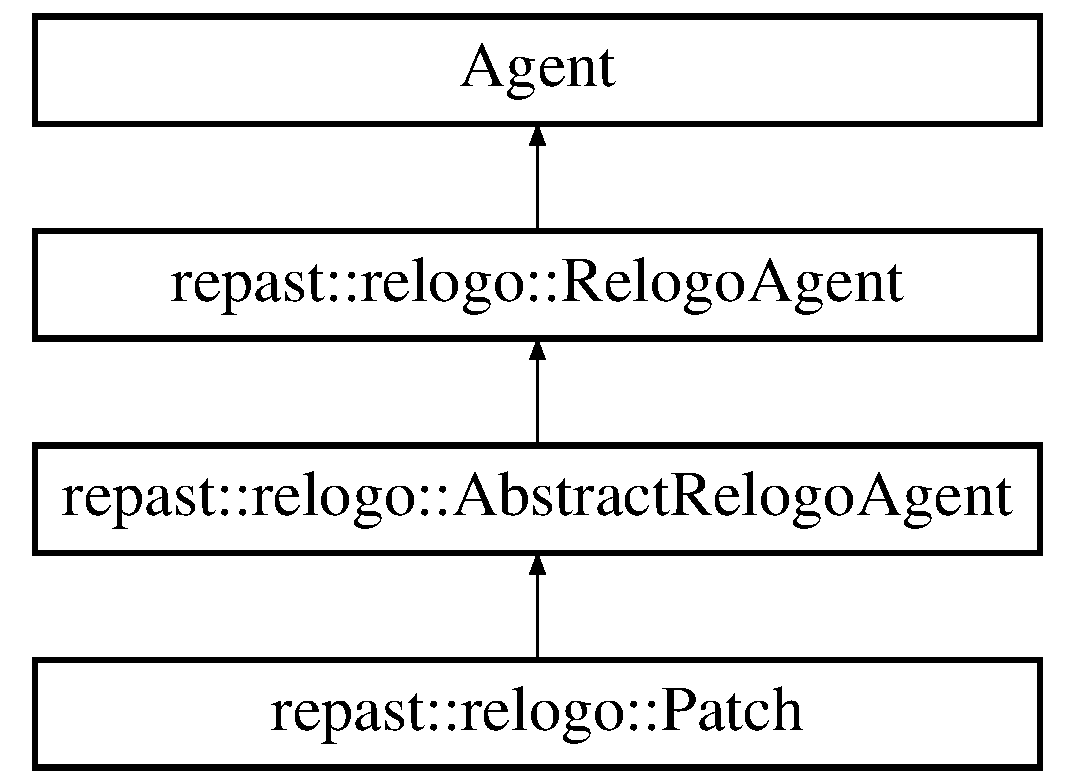
\includegraphics[height=4.000000cm]{classrepast_1_1relogo_1_1_patch}
\end{center}
\end{figure}
\subsection*{Public Member Functions}
\begin{DoxyCompactItemize}
\item 
\hyperlink{classrepast_1_1relogo_1_1_patch_aa866832379645e38ccd420e91c0fe7d0}{Patch} (repast\-::\-Agent\-Id id, \hyperlink{classrepast_1_1relogo_1_1_observer}{Observer} $\ast$observer)
\begin{DoxyCompactList}\small\item\em Creates a \hyperlink{classrepast_1_1relogo_1_1_patch}{Patch} that will have the specified id and be managed by the specified \hyperlink{classrepast_1_1relogo_1_1_observer}{Observer}. \end{DoxyCompactList}\item 
\hypertarget{classrepast_1_1relogo_1_1_patch_a410a47c2b1dc260d83c65ffb66b33a75}{virtual int \hyperlink{classrepast_1_1relogo_1_1_patch_a410a47c2b1dc260d83c65ffb66b33a75}{px\-Cor} () const }\label{classrepast_1_1relogo_1_1_patch_a410a47c2b1dc260d83c65ffb66b33a75}

\begin{DoxyCompactList}\small\item\em Gets the patch x coordinate of this patch's location. \end{DoxyCompactList}\item 
\hypertarget{classrepast_1_1relogo_1_1_patch_a9fe953832fa384a6fa19bd32511954fc}{virtual int \hyperlink{classrepast_1_1relogo_1_1_patch_a9fe953832fa384a6fa19bd32511954fc}{py\-Cor} () const }\label{classrepast_1_1relogo_1_1_patch_a9fe953832fa384a6fa19bd32511954fc}

\begin{DoxyCompactList}\small\item\em Gets the patch y coordinate of this patch's location. \end{DoxyCompactList}\item 
{\footnotesize template$<$typename Patch\-Type $>$ }\\\hyperlink{classrepast_1_1relogo_1_1_agent_set}{Agent\-Set}$<$ Patch\-Type $>$ \hyperlink{classrepast_1_1relogo_1_1_patch_a932368812cacb950454ceec64bf621e1}{neighbors} ()
\begin{DoxyCompactList}\small\item\em Gets the 8 (Moore neighborhood) neighboring Patches of this \hyperlink{classrepast_1_1relogo_1_1_patch}{Patch}. \end{DoxyCompactList}\item 
{\footnotesize template$<$typename Patch\-Type $>$ }\\\hyperlink{classrepast_1_1relogo_1_1_agent_set}{Agent\-Set}$<$ Patch\-Type $>$ \hyperlink{classrepast_1_1relogo_1_1_patch_a0e372725c27abb4e9b2b6ae61cfc4540}{neighbors4} ()
\begin{DoxyCompactList}\small\item\em Gets the 4 (Von Neumann neighborhood) neighboring Patches of this \hyperlink{classrepast_1_1relogo_1_1_patch}{Patch}. \end{DoxyCompactList}\item 
{\footnotesize template$<$typename Patch\-Type $>$ }\\void \hyperlink{classrepast_1_1relogo_1_1_patch_a23f5d9dbecd26acb74d71bd05c36ce77}{neighbors} (\hyperlink{classrepast_1_1relogo_1_1_agent_set}{Agent\-Set}$<$ Patch\-Type $>$ \&out)
\begin{DoxyCompactList}\small\item\em Gets the 8 (Moore neighborhood) neighboring Patches of this \hyperlink{classrepast_1_1relogo_1_1_patch}{Patch} and puts them out. \end{DoxyCompactList}\item 
{\footnotesize template$<$typename Patch\-Type $>$ }\\void \hyperlink{classrepast_1_1relogo_1_1_patch_aa157e0a9f7028a911a7abde580889511}{neighbors4} (\hyperlink{classrepast_1_1relogo_1_1_agent_set}{Agent\-Set}$<$ Patch\-Type $>$ \&out)
\begin{DoxyCompactList}\small\item\em Gets the 4 (Von Neumann neighborhood) neighboring Patches of this \hyperlink{classrepast_1_1relogo_1_1_patch}{Patch}. \end{DoxyCompactList}\end{DoxyCompactItemize}


\subsection{Detailed Description}
A logo patch. 

\subsection{Constructor \& Destructor Documentation}
\hypertarget{classrepast_1_1relogo_1_1_patch_aa866832379645e38ccd420e91c0fe7d0}{\index{repast\-::relogo\-::\-Patch@{repast\-::relogo\-::\-Patch}!Patch@{Patch}}
\index{Patch@{Patch}!repast::relogo::Patch@{repast\-::relogo\-::\-Patch}}
\subsubsection[{Patch}]{\setlength{\rightskip}{0pt plus 5cm}repast\-::relogo\-::\-Patch\-::\-Patch (
\begin{DoxyParamCaption}
\item[{repast\-::\-Agent\-Id}]{id, }
\item[{{\bf Observer} $\ast$}]{observer}
\end{DoxyParamCaption}
)}}\label{classrepast_1_1relogo_1_1_patch_aa866832379645e38ccd420e91c0fe7d0}


Creates a \hyperlink{classrepast_1_1relogo_1_1_patch}{Patch} that will have the specified id and be managed by the specified \hyperlink{classrepast_1_1relogo_1_1_observer}{Observer}. 


\begin{DoxyParams}{Parameters}
{\em id} & \\
\hline
{\em observer} & \\
\hline
\end{DoxyParams}


\subsection{Member Function Documentation}
\hypertarget{classrepast_1_1relogo_1_1_patch_a932368812cacb950454ceec64bf621e1}{\index{repast\-::relogo\-::\-Patch@{repast\-::relogo\-::\-Patch}!neighbors@{neighbors}}
\index{neighbors@{neighbors}!repast::relogo::Patch@{repast\-::relogo\-::\-Patch}}
\subsubsection[{neighbors}]{\setlength{\rightskip}{0pt plus 5cm}template$<$typename Patch\-Type $>$ {\bf Agent\-Set}$<$ Patch\-Type $>$ repast\-::relogo\-::\-Patch\-::neighbors (
\begin{DoxyParamCaption}
{}
\end{DoxyParamCaption}
)}}\label{classrepast_1_1relogo_1_1_patch_a932368812cacb950454ceec64bf621e1}


Gets the 8 (Moore neighborhood) neighboring Patches of this \hyperlink{classrepast_1_1relogo_1_1_patch}{Patch}. 


\begin{DoxyTemplParams}{Template Parameters}
{\em the} & patch type \\
\hline
\end{DoxyTemplParams}
\begin{DoxyReturn}{Returns}
the 8 (Moore neighborhood) neighboring Patches of this \hyperlink{classrepast_1_1relogo_1_1_patch}{Patch}. 
\end{DoxyReturn}
\hypertarget{classrepast_1_1relogo_1_1_patch_a23f5d9dbecd26acb74d71bd05c36ce77}{\index{repast\-::relogo\-::\-Patch@{repast\-::relogo\-::\-Patch}!neighbors@{neighbors}}
\index{neighbors@{neighbors}!repast::relogo::Patch@{repast\-::relogo\-::\-Patch}}
\subsubsection[{neighbors}]{\setlength{\rightskip}{0pt plus 5cm}template$<$typename Patch\-Type $>$ void repast\-::relogo\-::\-Patch\-::neighbors (
\begin{DoxyParamCaption}
\item[{{\bf Agent\-Set}$<$ Patch\-Type $>$ \&}]{out}
\end{DoxyParamCaption}
)}}\label{classrepast_1_1relogo_1_1_patch_a23f5d9dbecd26acb74d71bd05c36ce77}


Gets the 8 (Moore neighborhood) neighboring Patches of this \hyperlink{classrepast_1_1relogo_1_1_patch}{Patch} and puts them out. 


\begin{DoxyParams}{Parameters}
{\em out} & the \hyperlink{classrepast_1_1relogo_1_1_agent_set}{Agent\-Set} to the neighbors in \\
\hline
\end{DoxyParams}

\begin{DoxyTemplParams}{Template Parameters}
{\em the} & patch type \\
\hline
\end{DoxyTemplParams}
\hypertarget{classrepast_1_1relogo_1_1_patch_a0e372725c27abb4e9b2b6ae61cfc4540}{\index{repast\-::relogo\-::\-Patch@{repast\-::relogo\-::\-Patch}!neighbors4@{neighbors4}}
\index{neighbors4@{neighbors4}!repast::relogo::Patch@{repast\-::relogo\-::\-Patch}}
\subsubsection[{neighbors4}]{\setlength{\rightskip}{0pt plus 5cm}template$<$typename Patch\-Type $>$ {\bf Agent\-Set}$<$ Patch\-Type $>$ repast\-::relogo\-::\-Patch\-::neighbors4 (
\begin{DoxyParamCaption}
{}
\end{DoxyParamCaption}
)}}\label{classrepast_1_1relogo_1_1_patch_a0e372725c27abb4e9b2b6ae61cfc4540}


Gets the 4 (Von Neumann neighborhood) neighboring Patches of this \hyperlink{classrepast_1_1relogo_1_1_patch}{Patch}. 


\begin{DoxyTemplParams}{Template Parameters}
{\em the} & patch type \\
\hline
\end{DoxyTemplParams}
\begin{DoxyReturn}{Returns}
the 4 (Von Neumann neighborhood) neighboring Patches of this \hyperlink{classrepast_1_1relogo_1_1_patch}{Patch}. 
\end{DoxyReturn}
\hypertarget{classrepast_1_1relogo_1_1_patch_aa157e0a9f7028a911a7abde580889511}{\index{repast\-::relogo\-::\-Patch@{repast\-::relogo\-::\-Patch}!neighbors4@{neighbors4}}
\index{neighbors4@{neighbors4}!repast::relogo::Patch@{repast\-::relogo\-::\-Patch}}
\subsubsection[{neighbors4}]{\setlength{\rightskip}{0pt plus 5cm}template$<$typename Patch\-Type $>$ void repast\-::relogo\-::\-Patch\-::neighbors4 (
\begin{DoxyParamCaption}
\item[{{\bf Agent\-Set}$<$ Patch\-Type $>$ \&}]{out}
\end{DoxyParamCaption}
)}}\label{classrepast_1_1relogo_1_1_patch_aa157e0a9f7028a911a7abde580889511}


Gets the 4 (Von Neumann neighborhood) neighboring Patches of this \hyperlink{classrepast_1_1relogo_1_1_patch}{Patch}. 


\begin{DoxyParams}{Parameters}
{\em out} & the \hyperlink{classrepast_1_1relogo_1_1_agent_set}{Agent\-Set} to put the neighbors in \\
\hline
\end{DoxyParams}

\begin{DoxyTemplParams}{Template Parameters}
{\em the} & patch type \\
\hline
\end{DoxyTemplParams}


The documentation for this class was generated from the following files\-:\begin{DoxyCompactItemize}
\item 
/\-Users/murphy/work/\-Repast\-H\-P\-C\-\_\-\-G\-I\-T/repast.\-hpc/src/relogo/Patch.\-h\item 
/\-Users/murphy/work/\-Repast\-H\-P\-C\-\_\-\-G\-I\-T/repast.\-hpc/src/relogo/Patch.\-cpp\end{DoxyCompactItemize}

\hypertarget{classrepast_1_1relogo_1_1_random_move}{\section{repast\-:\-:relogo\-:\-:Random\-Move Class Reference}
\label{classrepast_1_1relogo_1_1_random_move}\index{repast\-::relogo\-::\-Random\-Move@{repast\-::relogo\-::\-Random\-Move}}
}


Operator(() that implements random move for a turtle.  




{\ttfamily \#include $<$Random\-Move.\-h$>$}

\subsection*{Public Member Functions}
\begin{DoxyCompactItemize}
\item 
\hyperlink{classrepast_1_1relogo_1_1_random_move_a7fcb5ce02c9662176f7fab7cbb26f684}{Random\-Move} (\hyperlink{classrepast_1_1relogo_1_1_observer}{Observer} $\ast$observer)
\begin{DoxyCompactList}\small\item\em Creates a \hyperlink{classrepast_1_1relogo_1_1_random_move}{Random\-Move} that randomly move turtles within the spaces managed by the specified observer. \end{DoxyCompactList}\item 
void \hyperlink{classrepast_1_1relogo_1_1_random_move_ad6273ded4033465519583ba5f57cbe21}{operator()} (\hyperlink{classrepast_1_1relogo_1_1_turtle}{Turtle} $\ast$turtle) const 
\begin{DoxyCompactList}\small\item\em Move the specified turtle at random. \end{DoxyCompactList}\end{DoxyCompactItemize}


\subsection{Detailed Description}
Operator(() that implements random move for a turtle. 

\subsection{Constructor \& Destructor Documentation}
\hypertarget{classrepast_1_1relogo_1_1_random_move_a7fcb5ce02c9662176f7fab7cbb26f684}{\index{repast\-::relogo\-::\-Random\-Move@{repast\-::relogo\-::\-Random\-Move}!Random\-Move@{Random\-Move}}
\index{Random\-Move@{Random\-Move}!repast::relogo::RandomMove@{repast\-::relogo\-::\-Random\-Move}}
\subsubsection[{Random\-Move}]{\setlength{\rightskip}{0pt plus 5cm}repast\-::relogo\-::\-Random\-Move\-::\-Random\-Move (
\begin{DoxyParamCaption}
\item[{{\bf Observer} $\ast$}]{observer}
\end{DoxyParamCaption}
)\hspace{0.3cm}{\ttfamily [inline]}}}\label{classrepast_1_1relogo_1_1_random_move_a7fcb5ce02c9662176f7fab7cbb26f684}


Creates a \hyperlink{classrepast_1_1relogo_1_1_random_move}{Random\-Move} that randomly move turtles within the spaces managed by the specified observer. 


\begin{DoxyParams}{Parameters}
{\em observer} & the observer whose spaces and turtles we want to move \\
\hline
\end{DoxyParams}


\subsection{Member Function Documentation}
\hypertarget{classrepast_1_1relogo_1_1_random_move_ad6273ded4033465519583ba5f57cbe21}{\index{repast\-::relogo\-::\-Random\-Move@{repast\-::relogo\-::\-Random\-Move}!operator()@{operator()}}
\index{operator()@{operator()}!repast::relogo::RandomMove@{repast\-::relogo\-::\-Random\-Move}}
\subsubsection[{operator()}]{\setlength{\rightskip}{0pt plus 5cm}void repast\-::relogo\-::\-Random\-Move\-::operator() (
\begin{DoxyParamCaption}
\item[{{\bf Turtle} $\ast$}]{turtle}
\end{DoxyParamCaption}
) const}}\label{classrepast_1_1relogo_1_1_random_move_ad6273ded4033465519583ba5f57cbe21}


Move the specified turtle at random. 


\begin{DoxyParams}{Parameters}
{\em turtle} & the turtel to move \\
\hline
\end{DoxyParams}


The documentation for this class was generated from the following files\-:\begin{DoxyCompactItemize}
\item 
/\-Users/murphy/work/\-Repast\-H\-P\-C\-\_\-\-G\-I\-T/repast.\-hpc/src/relogo/Random\-Move.\-h\item 
/\-Users/murphy/work/\-Repast\-H\-P\-C\-\_\-\-G\-I\-T/repast.\-hpc/src/relogo/Random\-Move.\-cpp\end{DoxyCompactItemize}

\hypertarget{classrepast_1_1relogo_1_1_relogo_agent}{\section{repast\-:\-:relogo\-:\-:Relogo\-Agent Class Reference}
\label{classrepast_1_1relogo_1_1_relogo_agent}\index{repast\-::relogo\-::\-Relogo\-Agent@{repast\-::relogo\-::\-Relogo\-Agent}}
}


Base agent for Relogo.  




{\ttfamily \#include $<$Relogo\-Agent.\-h$>$}

Inheritance diagram for repast\-:\-:relogo\-:\-:Relogo\-Agent\-:\begin{figure}[H]
\begin{center}
\leavevmode
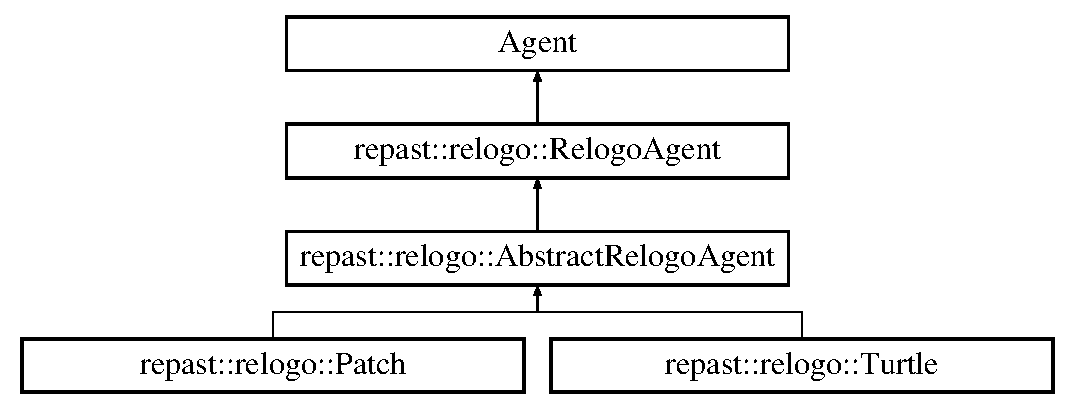
\includegraphics[height=4.000000cm]{classrepast_1_1relogo_1_1_relogo_agent}
\end{center}
\end{figure}
\subsection*{Public Member Functions}
\begin{DoxyCompactItemize}
\item 
\hyperlink{classrepast_1_1relogo_1_1_relogo_agent_a3a105277ddc72f3087738ebec3cf68e2}{Relogo\-Agent} (repast\-::\-Agent\-Id id, \hyperlink{classrepast_1_1relogo_1_1_observer}{Observer} $\ast$observer)
\begin{DoxyCompactList}\small\item\em Creates a \hyperlink{classrepast_1_1relogo_1_1_relogo_agent}{Relogo\-Agent} with the specified id and managed by the specified \hyperlink{classrepast_1_1relogo_1_1_observer}{Observer}. \end{DoxyCompactList}\item 
virtual repast\-::\-Agent\-Id \& \hyperlink{classrepast_1_1relogo_1_1_relogo_agent_a9df24a6bd58408f501512ee5c0921969}{get\-Id} ()
\begin{DoxyCompactList}\small\item\em Gets the id of this \hyperlink{classrepast_1_1relogo_1_1_relogo_agent}{Relogo\-Agent}. \end{DoxyCompactList}\item 
virtual const repast\-::\-Agent\-Id \& \hyperlink{classrepast_1_1relogo_1_1_relogo_agent_addc5c801304c04233158c731fffa6e0b}{get\-Id} () const 
\begin{DoxyCompactList}\small\item\em Gets the const id of this \hyperlink{classrepast_1_1relogo_1_1_relogo_agent}{Relogo\-Agent}. \end{DoxyCompactList}\item 
Point$<$ double $>$ \hyperlink{classrepast_1_1relogo_1_1_relogo_agent_a12632fc6c21f34dc1552a1d46d7d1000}{location} () const 
\begin{DoxyCompactList}\small\item\em Gets the location of this \hyperlink{classrepast_1_1relogo_1_1_relogo_agent}{Relogo\-Agent}. \end{DoxyCompactList}\item 
\hypertarget{classrepast_1_1relogo_1_1_relogo_agent_ad15d6628284018cf9d729a0d9953d5cb}{virtual void \hyperlink{classrepast_1_1relogo_1_1_relogo_agent_ad15d6628284018cf9d729a0d9953d5cb}{hatch\-Copy} ()}\label{classrepast_1_1relogo_1_1_relogo_agent_ad15d6628284018cf9d729a0d9953d5cb}

\begin{DoxyCompactList}\small\item\em If this Re\-Logo agent is 'hatched', makes an appropriate copy, setting instance variables as appropriate. \end{DoxyCompactList}\item 
double \hyperlink{classrepast_1_1relogo_1_1_relogo_agent_ad741eb80eea72c025089fc641cd6f9a5}{x\-Cor} () const 
\begin{DoxyCompactList}\small\item\em Gets the x coordinate of the agent's location. \end{DoxyCompactList}\item 
double \hyperlink{classrepast_1_1relogo_1_1_relogo_agent_ae9cff89b06acffb461a391ab4bd13206}{y\-Cor} () const 
\begin{DoxyCompactList}\small\item\em Gets the y coordinate of the agent's location. \end{DoxyCompactList}\item 
virtual int \hyperlink{classrepast_1_1relogo_1_1_relogo_agent_a8219a12f66709b4c86c547668235eda9}{px\-Cor} () const =0
\begin{DoxyCompactList}\small\item\em Gets the patch x coordinate of the agent's location. \end{DoxyCompactList}\item 
virtual int \hyperlink{classrepast_1_1relogo_1_1_relogo_agent_a4cf0eae31dc04149160dfd7b77044158}{py\-Cor} () const =0
\begin{DoxyCompactList}\small\item\em Gets the patch y coordinate of the agent's location. \end{DoxyCompactList}\item 
double \hyperlink{classrepast_1_1relogo_1_1_relogo_agent_a12a186ace28dcebf62faa6d3441f8a78}{distance} (\hyperlink{classrepast_1_1relogo_1_1_relogo_agent}{Relogo\-Agent} $\ast$obj) const 
\begin{DoxyCompactList}\small\item\em Gets the distance from this \hyperlink{classrepast_1_1relogo_1_1_relogo_agent}{Relogo\-Agent} to the specified agent. \end{DoxyCompactList}\item 
double \hyperlink{classrepast_1_1relogo_1_1_relogo_agent_a99dc8c0452c0fb699f7e807224e41d64}{distancexy} (double x, double y) const 
\begin{DoxyCompactList}\small\item\em Gets the distance from this \hyperlink{classrepast_1_1relogo_1_1_relogo_agent}{Relogo\-Agent} to the specified point. \end{DoxyCompactList}\end{DoxyCompactItemize}
\subsection*{Protected Attributes}
\begin{DoxyCompactItemize}
\item 
\hypertarget{classrepast_1_1relogo_1_1_relogo_agent_a1602e1180db11cdde666ac2beca0e0a2}{\hyperlink{classrepast_1_1relogo_1_1_observer}{Observer} $\ast$ {\bfseries \-\_\-observer}}\label{classrepast_1_1relogo_1_1_relogo_agent_a1602e1180db11cdde666ac2beca0e0a2}

\item 
\hypertarget{classrepast_1_1relogo_1_1_relogo_agent_ab71970dcf25d263c02b58ad645406f6f}{Point$<$ double $>$ {\bfseries \-\_\-location}}\label{classrepast_1_1relogo_1_1_relogo_agent_ab71970dcf25d263c02b58ad645406f6f}

\item 
\hypertarget{classrepast_1_1relogo_1_1_relogo_agent_a4745c9c678747f179ac788299da51983}{repast\-::\-Agent\-Id {\bfseries \-\_\-id}}\label{classrepast_1_1relogo_1_1_relogo_agent_a4745c9c678747f179ac788299da51983}

\end{DoxyCompactItemize}
\subsection*{Friends}
\begin{DoxyCompactItemize}
\item 
\hypertarget{classrepast_1_1relogo_1_1_relogo_agent_a9357229e3d8becac7ea9ce4fc821c8b6}{class {\bfseries Relogo\-Continuous\-Space\-Adder}}\label{classrepast_1_1relogo_1_1_relogo_agent_a9357229e3d8becac7ea9ce4fc821c8b6}

\item 
\hypertarget{classrepast_1_1relogo_1_1_relogo_agent_a8d256944f28ec0cd654da58d4dcff11c}{class {\bfseries World\-Creator}}\label{classrepast_1_1relogo_1_1_relogo_agent_a8d256944f28ec0cd654da58d4dcff11c}

\item 
\hypertarget{classrepast_1_1relogo_1_1_relogo_agent_a36ecfaff22237c775324f8e1db5b5610}{{\footnotesize template$<$typename G\-P\-Transformer , typename Adder $>$ }\\class {\bfseries Relogo\-Shared\-Continuous\-Space}}\label{classrepast_1_1relogo_1_1_relogo_agent_a36ecfaff22237c775324f8e1db5b5610}

\end{DoxyCompactItemize}


\subsection{Detailed Description}
Base agent for Relogo. 

\subsection{Constructor \& Destructor Documentation}
\hypertarget{classrepast_1_1relogo_1_1_relogo_agent_a3a105277ddc72f3087738ebec3cf68e2}{\index{repast\-::relogo\-::\-Relogo\-Agent@{repast\-::relogo\-::\-Relogo\-Agent}!Relogo\-Agent@{Relogo\-Agent}}
\index{Relogo\-Agent@{Relogo\-Agent}!repast::relogo::RelogoAgent@{repast\-::relogo\-::\-Relogo\-Agent}}
\subsubsection[{Relogo\-Agent}]{\setlength{\rightskip}{0pt plus 5cm}repast\-::relogo\-::\-Relogo\-Agent\-::\-Relogo\-Agent (
\begin{DoxyParamCaption}
\item[{repast\-::\-Agent\-Id}]{id, }
\item[{{\bf Observer} $\ast$}]{observer}
\end{DoxyParamCaption}
)\hspace{0.3cm}{\ttfamily [inline]}}}\label{classrepast_1_1relogo_1_1_relogo_agent_a3a105277ddc72f3087738ebec3cf68e2}


Creates a \hyperlink{classrepast_1_1relogo_1_1_relogo_agent}{Relogo\-Agent} with the specified id and managed by the specified \hyperlink{classrepast_1_1relogo_1_1_observer}{Observer}. 


\begin{DoxyParams}{Parameters}
{\em id} & the id of this \hyperlink{classrepast_1_1relogo_1_1_relogo_agent}{Relogo\-Agent} \\
\hline
{\em observer} & the observer that will manage this agent. \\
\hline
\end{DoxyParams}


\subsection{Member Function Documentation}
\hypertarget{classrepast_1_1relogo_1_1_relogo_agent_a12a186ace28dcebf62faa6d3441f8a78}{\index{repast\-::relogo\-::\-Relogo\-Agent@{repast\-::relogo\-::\-Relogo\-Agent}!distance@{distance}}
\index{distance@{distance}!repast::relogo::RelogoAgent@{repast\-::relogo\-::\-Relogo\-Agent}}
\subsubsection[{distance}]{\setlength{\rightskip}{0pt plus 5cm}double repast\-::relogo\-::\-Relogo\-Agent\-::distance (
\begin{DoxyParamCaption}
\item[{{\bf Relogo\-Agent} $\ast$}]{obj}
\end{DoxyParamCaption}
) const}}\label{classrepast_1_1relogo_1_1_relogo_agent_a12a186ace28dcebf62faa6d3441f8a78}


Gets the distance from this \hyperlink{classrepast_1_1relogo_1_1_relogo_agent}{Relogo\-Agent} to the specified agent. 

\begin{DoxyReturn}{Returns}
the distance from this \hyperlink{classrepast_1_1relogo_1_1_relogo_agent}{Relogo\-Agent} to the specified agent. 
\end{DoxyReturn}
\hypertarget{classrepast_1_1relogo_1_1_relogo_agent_a99dc8c0452c0fb699f7e807224e41d64}{\index{repast\-::relogo\-::\-Relogo\-Agent@{repast\-::relogo\-::\-Relogo\-Agent}!distancexy@{distancexy}}
\index{distancexy@{distancexy}!repast::relogo::RelogoAgent@{repast\-::relogo\-::\-Relogo\-Agent}}
\subsubsection[{distancexy}]{\setlength{\rightskip}{0pt plus 5cm}double repast\-::relogo\-::\-Relogo\-Agent\-::distancexy (
\begin{DoxyParamCaption}
\item[{double}]{x, }
\item[{double}]{y}
\end{DoxyParamCaption}
) const}}\label{classrepast_1_1relogo_1_1_relogo_agent_a99dc8c0452c0fb699f7e807224e41d64}


Gets the distance from this \hyperlink{classrepast_1_1relogo_1_1_relogo_agent}{Relogo\-Agent} to the specified point. 

\begin{DoxyReturn}{Returns}
the distance from this \hyperlink{classrepast_1_1relogo_1_1_relogo_agent}{Relogo\-Agent} to the specified point. 
\end{DoxyReturn}
\hypertarget{classrepast_1_1relogo_1_1_relogo_agent_a9df24a6bd58408f501512ee5c0921969}{\index{repast\-::relogo\-::\-Relogo\-Agent@{repast\-::relogo\-::\-Relogo\-Agent}!get\-Id@{get\-Id}}
\index{get\-Id@{get\-Id}!repast::relogo::RelogoAgent@{repast\-::relogo\-::\-Relogo\-Agent}}
\subsubsection[{get\-Id}]{\setlength{\rightskip}{0pt plus 5cm}virtual repast\-::\-Agent\-Id\& repast\-::relogo\-::\-Relogo\-Agent\-::get\-Id (
\begin{DoxyParamCaption}
{}
\end{DoxyParamCaption}
)\hspace{0.3cm}{\ttfamily [inline]}, {\ttfamily [virtual]}}}\label{classrepast_1_1relogo_1_1_relogo_agent_a9df24a6bd58408f501512ee5c0921969}


Gets the id of this \hyperlink{classrepast_1_1relogo_1_1_relogo_agent}{Relogo\-Agent}. 

\begin{DoxyReturn}{Returns}
the id of this \hyperlink{classrepast_1_1relogo_1_1_relogo_agent}{Relogo\-Agent}. 
\end{DoxyReturn}
\hypertarget{classrepast_1_1relogo_1_1_relogo_agent_addc5c801304c04233158c731fffa6e0b}{\index{repast\-::relogo\-::\-Relogo\-Agent@{repast\-::relogo\-::\-Relogo\-Agent}!get\-Id@{get\-Id}}
\index{get\-Id@{get\-Id}!repast::relogo::RelogoAgent@{repast\-::relogo\-::\-Relogo\-Agent}}
\subsubsection[{get\-Id}]{\setlength{\rightskip}{0pt plus 5cm}virtual const repast\-::\-Agent\-Id\& repast\-::relogo\-::\-Relogo\-Agent\-::get\-Id (
\begin{DoxyParamCaption}
{}
\end{DoxyParamCaption}
) const\hspace{0.3cm}{\ttfamily [inline]}, {\ttfamily [virtual]}}}\label{classrepast_1_1relogo_1_1_relogo_agent_addc5c801304c04233158c731fffa6e0b}


Gets the const id of this \hyperlink{classrepast_1_1relogo_1_1_relogo_agent}{Relogo\-Agent}. 

\begin{DoxyReturn}{Returns}
the const id of this \hyperlink{classrepast_1_1relogo_1_1_relogo_agent}{Relogo\-Agent}. 
\end{DoxyReturn}
\hypertarget{classrepast_1_1relogo_1_1_relogo_agent_a12632fc6c21f34dc1552a1d46d7d1000}{\index{repast\-::relogo\-::\-Relogo\-Agent@{repast\-::relogo\-::\-Relogo\-Agent}!location@{location}}
\index{location@{location}!repast::relogo::RelogoAgent@{repast\-::relogo\-::\-Relogo\-Agent}}
\subsubsection[{location}]{\setlength{\rightskip}{0pt plus 5cm}Point$<$double$>$ repast\-::relogo\-::\-Relogo\-Agent\-::location (
\begin{DoxyParamCaption}
{}
\end{DoxyParamCaption}
) const\hspace{0.3cm}{\ttfamily [inline]}}}\label{classrepast_1_1relogo_1_1_relogo_agent_a12632fc6c21f34dc1552a1d46d7d1000}


Gets the location of this \hyperlink{classrepast_1_1relogo_1_1_relogo_agent}{Relogo\-Agent}. 

\begin{DoxyReturn}{Returns}
the location of this \hyperlink{classrepast_1_1relogo_1_1_relogo_agent}{Relogo\-Agent}. 
\end{DoxyReturn}
\hypertarget{classrepast_1_1relogo_1_1_relogo_agent_a8219a12f66709b4c86c547668235eda9}{\index{repast\-::relogo\-::\-Relogo\-Agent@{repast\-::relogo\-::\-Relogo\-Agent}!px\-Cor@{px\-Cor}}
\index{px\-Cor@{px\-Cor}!repast::relogo::RelogoAgent@{repast\-::relogo\-::\-Relogo\-Agent}}
\subsubsection[{px\-Cor}]{\setlength{\rightskip}{0pt plus 5cm}virtual int repast\-::relogo\-::\-Relogo\-Agent\-::px\-Cor (
\begin{DoxyParamCaption}
{}
\end{DoxyParamCaption}
) const\hspace{0.3cm}{\ttfamily [pure virtual]}}}\label{classrepast_1_1relogo_1_1_relogo_agent_a8219a12f66709b4c86c547668235eda9}


Gets the patch x coordinate of the agent's location. 

\begin{DoxyReturn}{Returns}
the patch x coordinate of the agent's location. 
\end{DoxyReturn}


Implemented in \hyperlink{classrepast_1_1relogo_1_1_turtle_abeb7b773c8c9d403317587a7acdc1c1f}{repast\-::relogo\-::\-Turtle}, \hyperlink{classrepast_1_1relogo_1_1_patch_a410a47c2b1dc260d83c65ffb66b33a75}{repast\-::relogo\-::\-Patch}, and \hyperlink{classrepast_1_1relogo_1_1_abstract_relogo_agent_ae631f45eba5815470dea5a2059213c1b}{repast\-::relogo\-::\-Abstract\-Relogo\-Agent}.

\hypertarget{classrepast_1_1relogo_1_1_relogo_agent_a4cf0eae31dc04149160dfd7b77044158}{\index{repast\-::relogo\-::\-Relogo\-Agent@{repast\-::relogo\-::\-Relogo\-Agent}!py\-Cor@{py\-Cor}}
\index{py\-Cor@{py\-Cor}!repast::relogo::RelogoAgent@{repast\-::relogo\-::\-Relogo\-Agent}}
\subsubsection[{py\-Cor}]{\setlength{\rightskip}{0pt plus 5cm}virtual int repast\-::relogo\-::\-Relogo\-Agent\-::py\-Cor (
\begin{DoxyParamCaption}
{}
\end{DoxyParamCaption}
) const\hspace{0.3cm}{\ttfamily [pure virtual]}}}\label{classrepast_1_1relogo_1_1_relogo_agent_a4cf0eae31dc04149160dfd7b77044158}


Gets the patch y coordinate of the agent's location. 

\begin{DoxyReturn}{Returns}
the patch y coordinate of the agent's location. 
\end{DoxyReturn}


Implemented in \hyperlink{classrepast_1_1relogo_1_1_turtle_a378a3a80d2d33e389d8d78f0e0cae6d2}{repast\-::relogo\-::\-Turtle}, \hyperlink{classrepast_1_1relogo_1_1_patch_a9fe953832fa384a6fa19bd32511954fc}{repast\-::relogo\-::\-Patch}, and \hyperlink{classrepast_1_1relogo_1_1_abstract_relogo_agent_a38df42fbb6277fa62d0068fbd37e6595}{repast\-::relogo\-::\-Abstract\-Relogo\-Agent}.

\hypertarget{classrepast_1_1relogo_1_1_relogo_agent_ad741eb80eea72c025089fc641cd6f9a5}{\index{repast\-::relogo\-::\-Relogo\-Agent@{repast\-::relogo\-::\-Relogo\-Agent}!x\-Cor@{x\-Cor}}
\index{x\-Cor@{x\-Cor}!repast::relogo::RelogoAgent@{repast\-::relogo\-::\-Relogo\-Agent}}
\subsubsection[{x\-Cor}]{\setlength{\rightskip}{0pt plus 5cm}double repast\-::relogo\-::\-Relogo\-Agent\-::x\-Cor (
\begin{DoxyParamCaption}
{}
\end{DoxyParamCaption}
) const}}\label{classrepast_1_1relogo_1_1_relogo_agent_ad741eb80eea72c025089fc641cd6f9a5}


Gets the x coordinate of the agent's location. 

\begin{DoxyReturn}{Returns}
the x coordinate of the agent's location. 
\end{DoxyReturn}
\hypertarget{classrepast_1_1relogo_1_1_relogo_agent_ae9cff89b06acffb461a391ab4bd13206}{\index{repast\-::relogo\-::\-Relogo\-Agent@{repast\-::relogo\-::\-Relogo\-Agent}!y\-Cor@{y\-Cor}}
\index{y\-Cor@{y\-Cor}!repast::relogo::RelogoAgent@{repast\-::relogo\-::\-Relogo\-Agent}}
\subsubsection[{y\-Cor}]{\setlength{\rightskip}{0pt plus 5cm}double repast\-::relogo\-::\-Relogo\-Agent\-::y\-Cor (
\begin{DoxyParamCaption}
{}
\end{DoxyParamCaption}
) const}}\label{classrepast_1_1relogo_1_1_relogo_agent_ae9cff89b06acffb461a391ab4bd13206}


Gets the y coordinate of the agent's location. 

\begin{DoxyReturn}{Returns}
the y coordinate of the agent's location. 
\end{DoxyReturn}


The documentation for this class was generated from the following files\-:\begin{DoxyCompactItemize}
\item 
/\-Users/murphy/work/\-Repast\-H\-P\-C\-\_\-\-G\-I\-T/repast.\-hpc/src/relogo/Relogo\-Agent.\-h\item 
/\-Users/murphy/work/\-Repast\-H\-P\-C\-\_\-\-G\-I\-T/repast.\-hpc/src/relogo/Relogo\-Agent.\-cpp\end{DoxyCompactItemize}

\hypertarget{classrepast_1_1relogo_1_1_relogo_continuous_space_adder}{\section{repast\-:\-:relogo\-:\-:Relogo\-Continuous\-Space\-Adder Class Reference}
\label{classrepast_1_1relogo_1_1_relogo_continuous_space_adder}\index{repast\-::relogo\-::\-Relogo\-Continuous\-Space\-Adder@{repast\-::relogo\-::\-Relogo\-Continuous\-Space\-Adder}}
}


An \char`\"{}\-Adder\char`\"{} for adding Relogo\-Agents to Relogo\-Spaces.  




{\ttfamily \#include $<$Relogo\-Continuous\-Space\-Adder.\-h$>$}

\subsection*{Public Member Functions}
\begin{DoxyCompactItemize}
\item 
\hypertarget{classrepast_1_1relogo_1_1_relogo_continuous_space_adder_ae3d1f3a8f4b28aaf125a2f958cd9d93d}{void {\bfseries init} (Grid\-Dimensions dimensions, Relogo\-Space\-Type $\ast$grid)}\label{classrepast_1_1relogo_1_1_relogo_continuous_space_adder_ae3d1f3a8f4b28aaf125a2f958cd9d93d}

\item 
\hypertarget{classrepast_1_1relogo_1_1_relogo_continuous_space_adder_a1f01bacbabf806b87c75c3a2c0631b48}{bool {\bfseries add} (boost\-::shared\-\_\-ptr$<$ \hyperlink{classrepast_1_1relogo_1_1_relogo_agent}{Relogo\-Agent} $>$ agent)}\label{classrepast_1_1relogo_1_1_relogo_continuous_space_adder_a1f01bacbabf806b87c75c3a2c0631b48}

\end{DoxyCompactItemize}


\subsection{Detailed Description}
An \char`\"{}\-Adder\char`\"{} for adding Relogo\-Agents to Relogo\-Spaces. 

The documentation for this class was generated from the following files\-:\begin{DoxyCompactItemize}
\item 
/\-Users/murphy/work/\-Repast\-H\-P\-C\-\_\-\-G\-I\-T/repast.\-hpc/src/relogo/Relogo\-Continuous\-Space\-Adder.\-h\item 
/\-Users/murphy/work/\-Repast\-H\-P\-C\-\_\-\-G\-I\-T/repast.\-hpc/src/relogo/Relogo\-Continuous\-Space\-Adder.\-cpp\end{DoxyCompactItemize}

\hypertarget{classrepast_1_1relogo_1_1_relogo_discrete_space_adder}{\section{repast\-:\-:relogo\-:\-:Relogo\-Discrete\-Space\-Adder Class Reference}
\label{classrepast_1_1relogo_1_1_relogo_discrete_space_adder}\index{repast\-::relogo\-::\-Relogo\-Discrete\-Space\-Adder@{repast\-::relogo\-::\-Relogo\-Discrete\-Space\-Adder}}
}


Adds Relogo\-Agents to Relogo\-Discrete\-Spaces.  




{\ttfamily \#include $<$Relogo\-Discrete\-Space\-Adder.\-h$>$}

\subsection*{Public Member Functions}
\begin{DoxyCompactItemize}
\item 
\hypertarget{classrepast_1_1relogo_1_1_relogo_discrete_space_adder_ac8700b679f36c3a2d6fd337567763bd2}{void {\bfseries init} (Grid\-Dimensions dimensions, Relogo\-Grid\-Type $\ast$grid)}\label{classrepast_1_1relogo_1_1_relogo_discrete_space_adder_ac8700b679f36c3a2d6fd337567763bd2}

\item 
\hypertarget{classrepast_1_1relogo_1_1_relogo_discrete_space_adder_ab37d7d2fcbe6543ccd55526c4342ec58}{bool {\bfseries add} (boost\-::shared\-\_\-ptr$<$ \hyperlink{classrepast_1_1relogo_1_1_relogo_agent}{Relogo\-Agent} $>$ agent)}\label{classrepast_1_1relogo_1_1_relogo_discrete_space_adder_ab37d7d2fcbe6543ccd55526c4342ec58}

\end{DoxyCompactItemize}


\subsection{Detailed Description}
Adds Relogo\-Agents to Relogo\-Discrete\-Spaces. 

The documentation for this class was generated from the following files\-:\begin{DoxyCompactItemize}
\item 
/\-Users/murphy/work/\-Repast\-H\-P\-C\-\_\-\-G\-I\-T/repast.\-hpc/src/relogo/Relogo\-Discrete\-Space\-Adder.\-h\item 
/\-Users/murphy/work/\-Repast\-H\-P\-C\-\_\-\-G\-I\-T/repast.\-hpc/src/relogo/Relogo\-Discrete\-Space\-Adder.\-cpp\end{DoxyCompactItemize}

\hypertarget{classrepast_1_1relogo_1_1_relogo_link}{\section{repast\-:\-:relogo\-:\-:Relogo\-Link Class Reference}
\label{classrepast_1_1relogo_1_1_relogo_link}\index{repast\-::relogo\-::\-Relogo\-Link@{repast\-::relogo\-::\-Relogo\-Link}}
}


Network link for Relogo.  




{\ttfamily \#include $<$Relogo\-Link.\-h$>$}

Inheritance diagram for repast\-:\-:relogo\-:\-:Relogo\-Link\-:\begin{figure}[H]
\begin{center}
\leavevmode
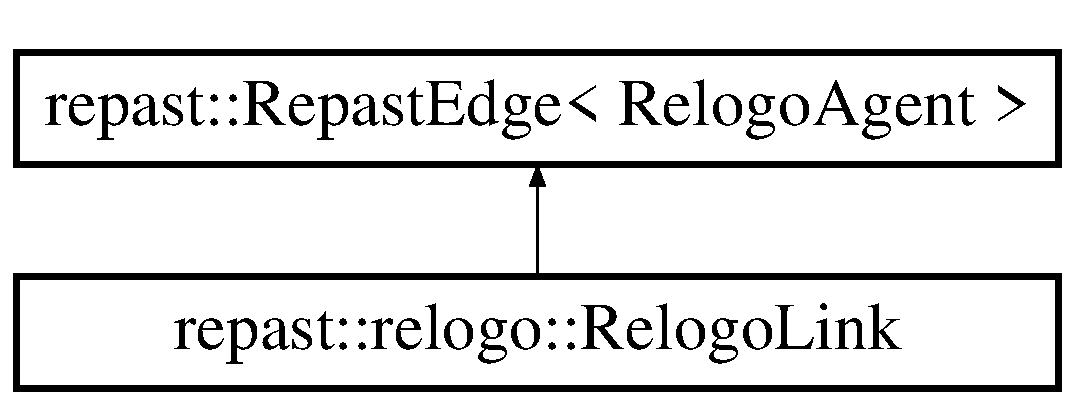
\includegraphics[height=2.000000cm]{classrepast_1_1relogo_1_1_relogo_link}
\end{center}
\end{figure}
\subsection*{Public Member Functions}
\begin{DoxyCompactItemize}
\item 
\hypertarget{classrepast_1_1relogo_1_1_relogo_link_aedbf01c7c5326863e179ceb2db1499bb}{\hyperlink{classrepast_1_1relogo_1_1_relogo_link_aedbf01c7c5326863e179ceb2db1499bb}{Relogo\-Link} ()}\label{classrepast_1_1relogo_1_1_relogo_link_aedbf01c7c5326863e179ceb2db1499bb}

\begin{DoxyCompactList}\small\item\em Creates an empty \hyperlink{classrepast_1_1relogo_1_1_relogo_link}{Relogo\-Link} with no source or target. \end{DoxyCompactList}\item 
\hyperlink{classrepast_1_1relogo_1_1_relogo_link_a56deff1fcae35290d55809fd92e7c99b}{Relogo\-Link} (\hyperlink{classrepast_1_1relogo_1_1_relogo_agent}{Relogo\-Agent} $\ast$source, \hyperlink{classrepast_1_1relogo_1_1_relogo_agent}{Relogo\-Agent} $\ast$target)
\begin{DoxyCompactList}\small\item\em Creates a \hyperlink{classrepast_1_1relogo_1_1_relogo_link}{Relogo\-Link} with the specified source and target and a default weight of 1. \end{DoxyCompactList}\item 
\hyperlink{classrepast_1_1relogo_1_1_relogo_link_a289496f5636c265ce5c8d8266029b8de}{Relogo\-Link} (\hyperlink{classrepast_1_1relogo_1_1_relogo_agent}{Relogo\-Agent} $\ast$source, \hyperlink{classrepast_1_1relogo_1_1_relogo_agent}{Relogo\-Agent} $\ast$target, double weight)
\begin{DoxyCompactList}\small\item\em Creates a \hyperlink{classrepast_1_1relogo_1_1_relogo_link}{Relogo\-Link} with the specified source, target, and weight. \end{DoxyCompactList}\item 
\hyperlink{classrepast_1_1relogo_1_1_relogo_link_aea1eb348b1a624d866a73f994c412f5e}{Relogo\-Link} (boost\-::shared\-\_\-ptr$<$ \hyperlink{classrepast_1_1relogo_1_1_relogo_agent}{Relogo\-Agent} $>$ source, boost\-::shared\-\_\-ptr$<$ \hyperlink{classrepast_1_1relogo_1_1_relogo_agent}{Relogo\-Agent} $>$ target)
\begin{DoxyCompactList}\small\item\em Creates a \hyperlink{classrepast_1_1relogo_1_1_relogo_link}{Relogo\-Link} with the specified source and target and a default weight of 1. \end{DoxyCompactList}\item 
\hyperlink{classrepast_1_1relogo_1_1_relogo_link_ab8860d71fe50d40e1c11fa4e53308581}{Relogo\-Link} (boost\-::shared\-\_\-ptr$<$ \hyperlink{classrepast_1_1relogo_1_1_relogo_agent}{Relogo\-Agent} $>$ source, boost\-::shared\-\_\-ptr$<$ \hyperlink{classrepast_1_1relogo_1_1_relogo_agent}{Relogo\-Agent} $>$ target, double weight)
\begin{DoxyCompactList}\small\item\em Creates a \hyperlink{classrepast_1_1relogo_1_1_relogo_link}{Relogo\-Link} with the specified source, target, and weight. \end{DoxyCompactList}\item 
\hypertarget{classrepast_1_1relogo_1_1_relogo_link_a3b6c85f36d32d9a416ee191fde225a6a}{\hyperlink{classrepast_1_1relogo_1_1_relogo_link_a3b6c85f36d32d9a416ee191fde225a6a}{Relogo\-Link} (const \hyperlink{classrepast_1_1relogo_1_1_relogo_link}{Relogo\-Link} \&edge)}\label{classrepast_1_1relogo_1_1_relogo_link_a3b6c85f36d32d9a416ee191fde225a6a}

\begin{DoxyCompactList}\small\item\em Copy constructor that creates a \hyperlink{classrepast_1_1relogo_1_1_relogo_link}{Relogo\-Link} from another \hyperlink{classrepast_1_1relogo_1_1_relogo_link}{Relogo\-Link}. \end{DoxyCompactList}\end{DoxyCompactItemize}


\subsection{Detailed Description}
Network link for Relogo. 

\subsection{Constructor \& Destructor Documentation}
\hypertarget{classrepast_1_1relogo_1_1_relogo_link_a56deff1fcae35290d55809fd92e7c99b}{\index{repast\-::relogo\-::\-Relogo\-Link@{repast\-::relogo\-::\-Relogo\-Link}!Relogo\-Link@{Relogo\-Link}}
\index{Relogo\-Link@{Relogo\-Link}!repast::relogo::RelogoLink@{repast\-::relogo\-::\-Relogo\-Link}}
\subsubsection[{Relogo\-Link}]{\setlength{\rightskip}{0pt plus 5cm}repast\-::relogo\-::\-Relogo\-Link\-::\-Relogo\-Link (
\begin{DoxyParamCaption}
\item[{{\bf Relogo\-Agent} $\ast$}]{source, }
\item[{{\bf Relogo\-Agent} $\ast$}]{target}
\end{DoxyParamCaption}
)}}\label{classrepast_1_1relogo_1_1_relogo_link_a56deff1fcae35290d55809fd92e7c99b}


Creates a \hyperlink{classrepast_1_1relogo_1_1_relogo_link}{Relogo\-Link} with the specified source and target and a default weight of 1. 


\begin{DoxyParams}{Parameters}
{\em source} & the link source \\
\hline
{\em target} & the link target \\
\hline
\end{DoxyParams}
\hypertarget{classrepast_1_1relogo_1_1_relogo_link_a289496f5636c265ce5c8d8266029b8de}{\index{repast\-::relogo\-::\-Relogo\-Link@{repast\-::relogo\-::\-Relogo\-Link}!Relogo\-Link@{Relogo\-Link}}
\index{Relogo\-Link@{Relogo\-Link}!repast::relogo::RelogoLink@{repast\-::relogo\-::\-Relogo\-Link}}
\subsubsection[{Relogo\-Link}]{\setlength{\rightskip}{0pt plus 5cm}repast\-::relogo\-::\-Relogo\-Link\-::\-Relogo\-Link (
\begin{DoxyParamCaption}
\item[{{\bf Relogo\-Agent} $\ast$}]{source, }
\item[{{\bf Relogo\-Agent} $\ast$}]{target, }
\item[{double}]{weight}
\end{DoxyParamCaption}
)}}\label{classrepast_1_1relogo_1_1_relogo_link_a289496f5636c265ce5c8d8266029b8de}


Creates a \hyperlink{classrepast_1_1relogo_1_1_relogo_link}{Relogo\-Link} with the specified source, target, and weight. 


\begin{DoxyParams}{Parameters}
{\em source} & the link source \\
\hline
{\em target} & the link target \\
\hline
{\em weight} & the link weight \\
\hline
\end{DoxyParams}
\hypertarget{classrepast_1_1relogo_1_1_relogo_link_aea1eb348b1a624d866a73f994c412f5e}{\index{repast\-::relogo\-::\-Relogo\-Link@{repast\-::relogo\-::\-Relogo\-Link}!Relogo\-Link@{Relogo\-Link}}
\index{Relogo\-Link@{Relogo\-Link}!repast::relogo::RelogoLink@{repast\-::relogo\-::\-Relogo\-Link}}
\subsubsection[{Relogo\-Link}]{\setlength{\rightskip}{0pt plus 5cm}repast\-::relogo\-::\-Relogo\-Link\-::\-Relogo\-Link (
\begin{DoxyParamCaption}
\item[{boost\-::shared\-\_\-ptr$<$ {\bf Relogo\-Agent} $>$}]{source, }
\item[{boost\-::shared\-\_\-ptr$<$ {\bf Relogo\-Agent} $>$}]{target}
\end{DoxyParamCaption}
)}}\label{classrepast_1_1relogo_1_1_relogo_link_aea1eb348b1a624d866a73f994c412f5e}


Creates a \hyperlink{classrepast_1_1relogo_1_1_relogo_link}{Relogo\-Link} with the specified source and target and a default weight of 1. 


\begin{DoxyParams}{Parameters}
{\em source} & the link source \\
\hline
{\em target} & the link target \\
\hline
\end{DoxyParams}
\hypertarget{classrepast_1_1relogo_1_1_relogo_link_ab8860d71fe50d40e1c11fa4e53308581}{\index{repast\-::relogo\-::\-Relogo\-Link@{repast\-::relogo\-::\-Relogo\-Link}!Relogo\-Link@{Relogo\-Link}}
\index{Relogo\-Link@{Relogo\-Link}!repast::relogo::RelogoLink@{repast\-::relogo\-::\-Relogo\-Link}}
\subsubsection[{Relogo\-Link}]{\setlength{\rightskip}{0pt plus 5cm}repast\-::relogo\-::\-Relogo\-Link\-::\-Relogo\-Link (
\begin{DoxyParamCaption}
\item[{boost\-::shared\-\_\-ptr$<$ {\bf Relogo\-Agent} $>$}]{source, }
\item[{boost\-::shared\-\_\-ptr$<$ {\bf Relogo\-Agent} $>$}]{target, }
\item[{double}]{weight}
\end{DoxyParamCaption}
)}}\label{classrepast_1_1relogo_1_1_relogo_link_ab8860d71fe50d40e1c11fa4e53308581}


Creates a \hyperlink{classrepast_1_1relogo_1_1_relogo_link}{Relogo\-Link} with the specified source, target, and weight. 


\begin{DoxyParams}{Parameters}
{\em source} & the link source \\
\hline
{\em target} & the link target \\
\hline
{\em weight} & the link weight \\
\hline
\end{DoxyParams}


The documentation for this class was generated from the following files\-:\begin{DoxyCompactItemize}
\item 
/\-Users/murphy/work/\-Repast\-H\-P\-C\-\_\-\-G\-I\-T/repast.\-hpc/src/relogo/Relogo\-Link.\-h\item 
/\-Users/murphy/work/\-Repast\-H\-P\-C\-\_\-\-G\-I\-T/repast.\-hpc/src/relogo/Relogo\-Link.\-cpp\end{DoxyCompactItemize}

\hypertarget{classrepast_1_1relogo_1_1_relogo_link_content}{\section{repast\-:\-:relogo\-:\-:Relogo\-Link\-Content Class Reference}
\label{classrepast_1_1relogo_1_1_relogo_link_content}\index{repast\-::relogo\-::\-Relogo\-Link\-Content@{repast\-::relogo\-::\-Relogo\-Link\-Content}}
}


Subclass of Repast\-Edge\-Content, used in synchronization.  




{\ttfamily \#include $<$Relogo\-Link.\-h$>$}

Inheritance diagram for repast\-:\-:relogo\-:\-:Relogo\-Link\-Content\-:\begin{figure}[H]
\begin{center}
\leavevmode
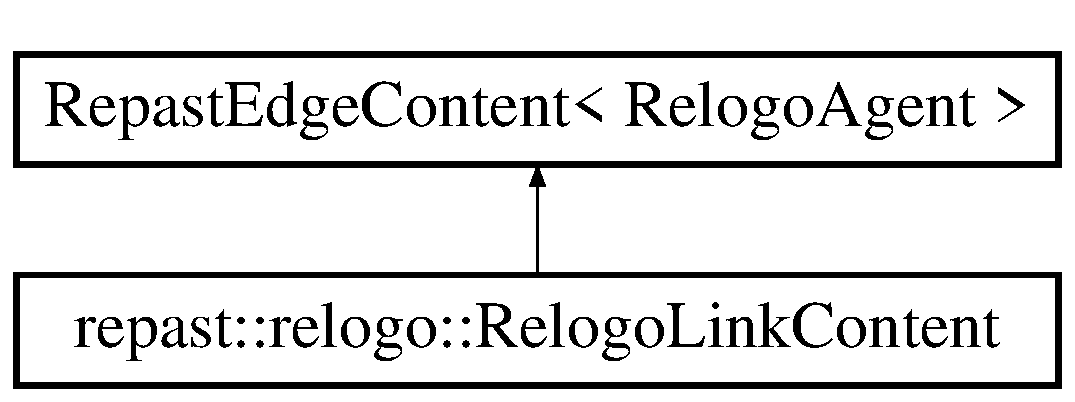
\includegraphics[height=2.000000cm]{classrepast_1_1relogo_1_1_relogo_link_content}
\end{center}
\end{figure}
\subsection*{Public Member Functions}
\begin{DoxyCompactItemize}
\item 
\hypertarget{classrepast_1_1relogo_1_1_relogo_link_content_a88617ac84e9e3b94419c0b240414bf59}{{\bfseries Relogo\-Link\-Content} (\hyperlink{classrepast_1_1relogo_1_1_relogo_link}{Relogo\-Link} $\ast$link)}\label{classrepast_1_1relogo_1_1_relogo_link_content_a88617ac84e9e3b94419c0b240414bf59}

\end{DoxyCompactItemize}


\subsection{Detailed Description}
Subclass of Repast\-Edge\-Content, used in synchronization. 

The documentation for this class was generated from the following file\-:\begin{DoxyCompactItemize}
\item 
/\-Users/murphy/work/\-Repast\-H\-P\-C\-\_\-\-G\-I\-T/repast.\-hpc/src/relogo/Relogo\-Link.\-h\end{DoxyCompactItemize}

\hypertarget{classrepast_1_1relogo_1_1_relogo_link_content_manager}{\section{repast\-:\-:relogo\-:\-:Relogo\-Link\-Content\-Manager Class Reference}
\label{classrepast_1_1relogo_1_1_relogo_link_content_manager}\index{repast\-::relogo\-::\-Relogo\-Link\-Content\-Manager@{repast\-::relogo\-::\-Relogo\-Link\-Content\-Manager}}
}


Subclass of Repast\-Edge\-Content\-Manager, used to package and rebuild edges during synchronization.  




{\ttfamily \#include $<$Relogo\-Link.\-h$>$}

\subsection*{Public Member Functions}
\begin{DoxyCompactItemize}
\item 
\hypertarget{classrepast_1_1relogo_1_1_relogo_link_content_manager_af34a2cc9aa6331c617de6e0af7a5eca4}{\hyperlink{classrepast_1_1relogo_1_1_relogo_link}{Relogo\-Link} $\ast$ {\bfseries create\-Edge} (\hyperlink{classrepast_1_1relogo_1_1_relogo_link_content}{Relogo\-Link\-Content} \&content, repast\-::\-Context$<$ \hyperlink{classrepast_1_1relogo_1_1_relogo_agent}{Relogo\-Agent} $>$ $\ast$context)}\label{classrepast_1_1relogo_1_1_relogo_link_content_manager_af34a2cc9aa6331c617de6e0af7a5eca4}

\item 
\hypertarget{classrepast_1_1relogo_1_1_relogo_link_content_manager_a4e85e7973518f8d58c0baaa2272f027e}{\hyperlink{classrepast_1_1relogo_1_1_relogo_link_content}{Relogo\-Link\-Content} $\ast$ {\bfseries provide\-Edge\-Content} (\hyperlink{classrepast_1_1relogo_1_1_relogo_link}{Relogo\-Link} $\ast$edge)}\label{classrepast_1_1relogo_1_1_relogo_link_content_manager_a4e85e7973518f8d58c0baaa2272f027e}

\end{DoxyCompactItemize}


\subsection{Detailed Description}
Subclass of Repast\-Edge\-Content\-Manager, used to package and rebuild edges during synchronization. 

The documentation for this class was generated from the following file\-:\begin{DoxyCompactItemize}
\item 
/\-Users/murphy/work/\-Repast\-H\-P\-C\-\_\-\-G\-I\-T/repast.\-hpc/src/relogo/Relogo\-Link.\-h\end{DoxyCompactItemize}

\hypertarget{classrepast_1_1relogo_1_1_relogo_shared_continuous_space}{\section{repast\-:\-:relogo\-:\-:Relogo\-Shared\-Continuous\-Space$<$ G\-P\-Transformer, Adder $>$ Class Template Reference}
\label{classrepast_1_1relogo_1_1_relogo_shared_continuous_space}\index{repast\-::relogo\-::\-Relogo\-Shared\-Continuous\-Space$<$ G\-P\-Transformer, Adder $>$@{repast\-::relogo\-::\-Relogo\-Shared\-Continuous\-Space$<$ G\-P\-Transformer, Adder $>$}}
}


Repast Shared\-Continuous\-Space specialized for Relogo.  




{\ttfamily \#include $<$Relogo\-Shared\-Continuous\-Space.\-h$>$}

Inheritance diagram for repast\-:\-:relogo\-:\-:Relogo\-Shared\-Continuous\-Space$<$ G\-P\-Transformer, Adder $>$\-:\begin{figure}[H]
\begin{center}
\leavevmode
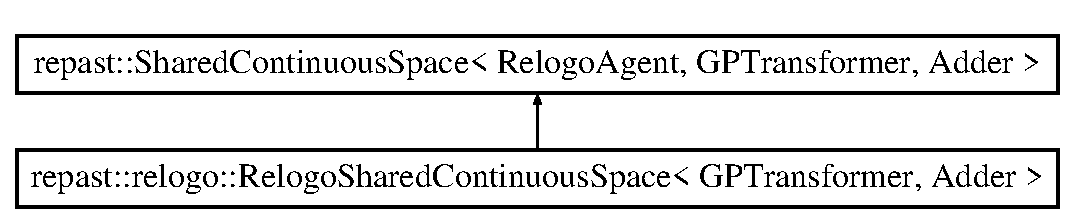
\includegraphics[height=2.000000cm]{classrepast_1_1relogo_1_1_relogo_shared_continuous_space}
\end{center}
\end{figure}
\subsection*{Public Member Functions}
\begin{DoxyCompactItemize}
\item 
\hypertarget{classrepast_1_1relogo_1_1_relogo_shared_continuous_space_ab7d25f7bcff3c09a10110ef9dfb01bdc}{{\bfseries Relogo\-Shared\-Continuous\-Space} (std\-::string name, repast\-::\-Grid\-Dimensions grid\-Dims, std\-::vector$<$ int $>$ process\-Dims, int buffer, boost\-::mpi\-::communicator $\ast$world)}\label{classrepast_1_1relogo_1_1_relogo_shared_continuous_space_ab7d25f7bcff3c09a10110ef9dfb01bdc}

\end{DoxyCompactItemize}
\subsection*{Protected Member Functions}
\begin{DoxyCompactItemize}
\item 
\hypertarget{classrepast_1_1relogo_1_1_relogo_shared_continuous_space_a0fae00be7a12e9080c9a945f2900f34f}{void {\bfseries synch\-Move\-To} (const repast\-::\-Agent\-Id \&id, const repast\-::\-Point$<$ double $>$ \&pt)}\label{classrepast_1_1relogo_1_1_relogo_shared_continuous_space_a0fae00be7a12e9080c9a945f2900f34f}

\end{DoxyCompactItemize}


\subsection{Detailed Description}
\subsubsection*{template$<$typename G\-P\-Transformer, typename Adder$>$class repast\-::relogo\-::\-Relogo\-Shared\-Continuous\-Space$<$ G\-P\-Transformer, Adder $>$}

Repast Shared\-Continuous\-Space specialized for Relogo. 

This overrides synch\-Move\-To. 

The documentation for this class was generated from the following files\-:\begin{DoxyCompactItemize}
\item 
/\-Users/murphy/work/\-Repast\-H\-P\-C\-\_\-\-G\-I\-T/repast.\-hpc/src/relogo/Relogo\-Agent.\-h\item 
/\-Users/murphy/work/\-Repast\-H\-P\-C\-\_\-\-G\-I\-T/repast.\-hpc/src/relogo/Relogo\-Shared\-Continuous\-Space.\-h\end{DoxyCompactItemize}

\hypertarget{classrepast_1_1relogo_1_1_relogo_shared_discrete_space}{\section{repast\-:\-:relogo\-:\-:Relogo\-Shared\-Discrete\-Space$<$ G\-P\-Transformer, Adder $>$ Class Template Reference}
\label{classrepast_1_1relogo_1_1_relogo_shared_discrete_space}\index{repast\-::relogo\-::\-Relogo\-Shared\-Discrete\-Space$<$ G\-P\-Transformer, Adder $>$@{repast\-::relogo\-::\-Relogo\-Shared\-Discrete\-Space$<$ G\-P\-Transformer, Adder $>$}}
}


Repast Shared\-Discrete\-Space specialized for Relogo.  




{\ttfamily \#include $<$Relogo\-Shared\-Discrete\-Space.\-h$>$}

Inheritance diagram for repast\-:\-:relogo\-:\-:Relogo\-Shared\-Discrete\-Space$<$ G\-P\-Transformer, Adder $>$\-:\begin{figure}[H]
\begin{center}
\leavevmode
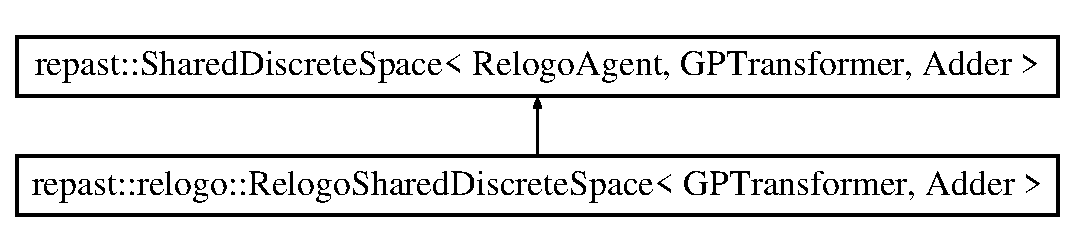
\includegraphics[height=2.000000cm]{classrepast_1_1relogo_1_1_relogo_shared_discrete_space}
\end{center}
\end{figure}
\subsection*{Public Member Functions}
\begin{DoxyCompactItemize}
\item 
\hypertarget{classrepast_1_1relogo_1_1_relogo_shared_discrete_space_afd6aadc89e1d8b95c451dcd7cdccf5d3}{{\bfseries Relogo\-Shared\-Discrete\-Space} (std\-::string name, repast\-::\-Grid\-Dimensions grid\-Dims, std\-::vector$<$ int $>$ process\-Dims, int buffer, boost\-::mpi\-::communicator $\ast$world)}\label{classrepast_1_1relogo_1_1_relogo_shared_discrete_space_afd6aadc89e1d8b95c451dcd7cdccf5d3}

\end{DoxyCompactItemize}


\subsection{Detailed Description}
\subsubsection*{template$<$typename G\-P\-Transformer, typename Adder$>$class repast\-::relogo\-::\-Relogo\-Shared\-Discrete\-Space$<$ G\-P\-Transformer, Adder $>$}

Repast Shared\-Discrete\-Space specialized for Relogo. 

The documentation for this class was generated from the following file\-:\begin{DoxyCompactItemize}
\item 
/\-Users/murphy/work/\-Repast\-H\-P\-C\-\_\-\-G\-I\-T/repast.\-hpc/src/relogo/Relogo\-Shared\-Discrete\-Space.\-h\end{DoxyCompactItemize}

\hypertarget{structrepast_1_1relogo_1_1_set_cmp}{\section{repast\-:\-:relogo\-:\-:Set\-Cmp$<$ T, Value\-Getter $>$ Struct Template Reference}
\label{structrepast_1_1relogo_1_1_set_cmp}\index{repast\-::relogo\-::\-Set\-Cmp$<$ T, Value\-Getter $>$@{repast\-::relogo\-::\-Set\-Cmp$<$ T, Value\-Getter $>$}}
}


Compares two items using the specified getter.  




{\ttfamily \#include $<$Agent\-Set.\-h$>$}

\subsection*{Public Member Functions}
\begin{DoxyCompactItemize}
\item 
\hypertarget{structrepast_1_1relogo_1_1_set_cmp_a43b579d59a9292f40fd24672090fca75}{{\bfseries Set\-Cmp} (const Value\-Getter $\ast$getter)}\label{structrepast_1_1relogo_1_1_set_cmp_a43b579d59a9292f40fd24672090fca75}

\item 
\hypertarget{structrepast_1_1relogo_1_1_set_cmp_a460d264b98975b66038a7cc0eead34a9}{bool {\bfseries operator()} (T $\ast$one, T $\ast$two)}\label{structrepast_1_1relogo_1_1_set_cmp_a460d264b98975b66038a7cc0eead34a9}

\end{DoxyCompactItemize}
\subsection*{Public Attributes}
\begin{DoxyCompactItemize}
\item 
\hypertarget{structrepast_1_1relogo_1_1_set_cmp_a26d5897fee7b4dee6f8735649cb4be23}{const Value\-Getter $\ast$ {\bfseries \-\_\-getter}}\label{structrepast_1_1relogo_1_1_set_cmp_a26d5897fee7b4dee6f8735649cb4be23}

\end{DoxyCompactItemize}


\subsection{Detailed Description}
\subsubsection*{template$<$typename T, typename Value\-Getter$>$struct repast\-::relogo\-::\-Set\-Cmp$<$ T, Value\-Getter $>$}

Compares two items using the specified getter. 

The documentation for this struct was generated from the following file\-:\begin{DoxyCompactItemize}
\item 
/\-Users/murphy/work/\-Repast\-H\-P\-C\-\_\-\-G\-I\-T/repast.\-hpc/src/relogo/Agent\-Set.\-h\end{DoxyCompactItemize}

\hypertarget{classrepast_1_1relogo_1_1_simulation_runner}{\section{repast\-:\-:relogo\-:\-:Simulation\-Runner Class Reference}
\label{classrepast_1_1relogo_1_1_simulation_runner}\index{repast\-::relogo\-::\-Simulation\-Runner@{repast\-::relogo\-::\-Simulation\-Runner}}
}


Runs a Relogo simulation.  




{\ttfamily \#include $<$Simulation\-Runner.\-h$>$}

\subsection*{Public Member Functions}
\begin{DoxyCompactItemize}
\item 
\hypertarget{classrepast_1_1relogo_1_1_simulation_runner_a728e64ef637008c47017cd351b8b067e}{\hyperlink{classrepast_1_1relogo_1_1_simulation_runner_a728e64ef637008c47017cd351b8b067e}{Simulation\-Runner} (boost\-::mpi\-::communicator $\ast$world)}\label{classrepast_1_1relogo_1_1_simulation_runner_a728e64ef637008c47017cd351b8b067e}

\begin{DoxyCompactList}\small\item\em Creates a \hyperlink{classrepast_1_1relogo_1_1_simulation_runner}{Simulation\-Runner}. \end{DoxyCompactList}\item 
{\footnotesize template$<$typename Observer\-Type , typename Patch\-Type $>$ }\\void \hyperlink{classrepast_1_1relogo_1_1_simulation_runner_ac5e8c7119f3278f5c64190e6686e59d0}{run} (Properties \&props)
\begin{DoxyCompactList}\small\item\em Creates and runs the simulation using the properties defined in props. \end{DoxyCompactList}\end{DoxyCompactItemize}
\subsection*{Protected Attributes}
\begin{DoxyCompactItemize}
\item 
\hypertarget{classrepast_1_1relogo_1_1_simulation_runner_a4d616014a9f755de2d32784e449629cf}{boost\-::mpi\-::communicator $\ast$ {\bfseries comm}}\label{classrepast_1_1relogo_1_1_simulation_runner_a4d616014a9f755de2d32784e449629cf}

\end{DoxyCompactItemize}


\subsection{Detailed Description}
Runs a Relogo simulation. 

\subsection{Member Function Documentation}
\hypertarget{classrepast_1_1relogo_1_1_simulation_runner_ac5e8c7119f3278f5c64190e6686e59d0}{\index{repast\-::relogo\-::\-Simulation\-Runner@{repast\-::relogo\-::\-Simulation\-Runner}!run@{run}}
\index{run@{run}!repast::relogo::SimulationRunner@{repast\-::relogo\-::\-Simulation\-Runner}}
\subsubsection[{run}]{\setlength{\rightskip}{0pt plus 5cm}template$<$typename Observer\-Type , typename Patch\-Type $>$ void repast\-::relogo\-::\-Simulation\-Runner\-::run (
\begin{DoxyParamCaption}
\item[{Properties \&}]{props}
\end{DoxyParamCaption}
)}}\label{classrepast_1_1relogo_1_1_simulation_runner_ac5e8c7119f3278f5c64190e6686e59d0}


Creates and runs the simulation using the properties defined in props. 

The properties file must have the following properties defined\-:


\begin{DoxyItemize}
\item min.\-x the minimum integer x coordinate of the world 
\item min.\-y the minimum integer y coordinate of the world 
\item max.\-x the maximum integer x coordinate of the world 
\item max.\-h the maximum integer y coordinate of the world 
\item grid.\-buffer the size of the grid and space buffers 
\item proc.\-per.\-x the number of processes to assign to the world's x dimension. proc.\-per.\-x multiplied by proc.\-per.\-y must equal the number processes that the simulation will run on 
\item proc.\-per.\-y the number of processes to assign to the world's y dimension. proc.\-per.\-x multiplied by proc.\-per.\-y must equal the number processes that the simulation will run on 
\item stop.\-at the tick at which to stop the simulation

This will create an \hyperlink{classrepast_1_1relogo_1_1_observer}{Observer} of the specified type and populate the world with Patches of the specified type. It will then call setup(props) on that \hyperlink{classrepast_1_1relogo_1_1_observer}{Observer} implementation and start the simulation schedule which will call the \hyperlink{classrepast_1_1relogo_1_1_observer}{Observer}'s go method each tick.


\begin{DoxyParams}{Parameters}
{\em props} & a properties file containing the properties mentioned above \\
\hline
\end{DoxyParams}

\begin{DoxyTemplParams}{Template Parameters}
{\em Observer\-Type} & the type of \hyperlink{classrepast_1_1relogo_1_1_observer}{Observer} to create. This type must extend \hyperlink{classrepast_1_1relogo_1_1_observer}{relogo\-::\-Observer}. \\
\hline
{\em Patch\-Type} & the type of Patches to create. This must extend \hyperlink{classrepast_1_1relogo_1_1_patch}{relogo\-::\-Patch}. \\
\hline
\end{DoxyTemplParams}

\end{DoxyItemize}

The documentation for this class was generated from the following file\-:\begin{DoxyCompactItemize}
\item 
/\-Users/murphy/work/\-Repast\-H\-P\-C\-\_\-\-G\-I\-T/repast.\-hpc/src/relogo/Simulation\-Runner.\-h\end{DoxyCompactItemize}

\hypertarget{classrepast_1_1relogo_1_1_turtle}{\section{repast\-:\-:relogo\-:\-:Turtle Class Reference}
\label{classrepast_1_1relogo_1_1_turtle}\index{repast\-::relogo\-::\-Turtle@{repast\-::relogo\-::\-Turtle}}
}


Relogo \hyperlink{classrepast_1_1relogo_1_1_turtle}{Turtle} implementation.  




{\ttfamily \#include $<$Turtle.\-h$>$}

Inheritance diagram for repast\-:\-:relogo\-:\-:Turtle\-:\begin{figure}[H]
\begin{center}
\leavevmode
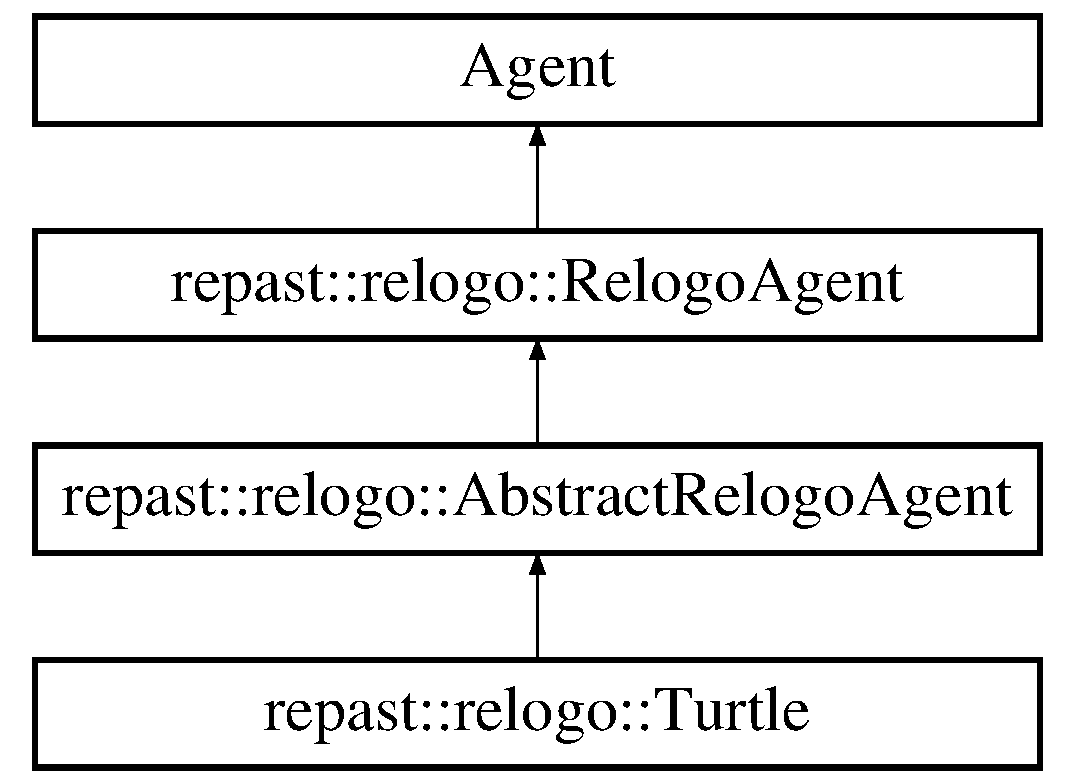
\includegraphics[height=4.000000cm]{classrepast_1_1relogo_1_1_turtle}
\end{center}
\end{figure}
\subsection*{Public Member Functions}
\begin{DoxyCompactItemize}
\item 
\hypertarget{classrepast_1_1relogo_1_1_turtle_aaa772cfde975ea37fa795c1cafdbb0df}{\hyperlink{classrepast_1_1relogo_1_1_turtle_aaa772cfde975ea37fa795c1cafdbb0df}{Turtle} (repast\-::\-Agent\-Id id, \hyperlink{classrepast_1_1relogo_1_1_observer}{Observer} $\ast$observer)}\label{classrepast_1_1relogo_1_1_turtle_aaa772cfde975ea37fa795c1cafdbb0df}

\begin{DoxyCompactList}\small\item\em Creates a \hyperlink{classrepast_1_1relogo_1_1_turtle}{Turtle} that will have the specified id, and be managed by the specified \hyperlink{classrepast_1_1relogo_1_1_observer}{Observer}. \end{DoxyCompactList}\item 
\hypertarget{classrepast_1_1relogo_1_1_turtle_a0995104470db5a506b8e5d5a2e29c45c}{virtual void {\bfseries hatch\-Copy} (\hyperlink{classrepast_1_1relogo_1_1_relogo_agent}{Relogo\-Agent} $\ast$parent)}\label{classrepast_1_1relogo_1_1_turtle_a0995104470db5a506b8e5d5a2e29c45c}

\item 
void \hyperlink{classrepast_1_1relogo_1_1_turtle_ad2fbb3478a37d234450362d8384fb457}{x\-Cor} (double x)
\begin{DoxyCompactList}\small\item\em Sets the x coordinate of the \hyperlink{classrepast_1_1relogo_1_1_turtle}{Turtle}'s location. \end{DoxyCompactList}\item 
void \hyperlink{classrepast_1_1relogo_1_1_turtle_a37b35041e28355a00a994fad94db0f0a}{y\-Cor} (double y)
\begin{DoxyCompactList}\small\item\em Sets the y coordinate of the \hyperlink{classrepast_1_1relogo_1_1_turtle}{Turtle}'s location. \end{DoxyCompactList}\item 
void \hyperlink{classrepast_1_1relogo_1_1_turtle_ab11fc0e94cfd9f414bd7c84022c9e4cd}{setxy} (double x, double y)
\begin{DoxyCompactList}\small\item\em Sets the x and y coordinate of the \hyperlink{classrepast_1_1relogo_1_1_turtle}{Turtle}'s location. \end{DoxyCompactList}\item 
virtual int \hyperlink{classrepast_1_1relogo_1_1_turtle_abeb7b773c8c9d403317587a7acdc1c1f}{px\-Cor} () const 
\begin{DoxyCompactList}\small\item\em Gets the \hyperlink{classrepast_1_1relogo_1_1_patch}{Patch} x coordinate of this \hyperlink{classrepast_1_1relogo_1_1_turtle}{Turtle}. \end{DoxyCompactList}\item 
virtual int \hyperlink{classrepast_1_1relogo_1_1_turtle_a378a3a80d2d33e389d8d78f0e0cae6d2}{py\-Cor} () const 
\begin{DoxyCompactList}\small\item\em Gets the \hyperlink{classrepast_1_1relogo_1_1_patch}{Patch} x coordinate of this \hyperlink{classrepast_1_1relogo_1_1_turtle}{Turtle}. \end{DoxyCompactList}\item 
void \hyperlink{classrepast_1_1relogo_1_1_turtle_aab4d6acd4379da5bcb778930403edcce}{die} ()
\begin{DoxyCompactList}\small\item\em Removes this turtle from the world. \end{DoxyCompactList}\item 
void \hyperlink{classrepast_1_1relogo_1_1_turtle_a9eb0244977fa479a1ddab9edf9cc7d96}{create\-Link\-With} (\hyperlink{classrepast_1_1relogo_1_1_turtle}{Turtle} $\ast$turtle, const std\-::string \&network=D\-E\-F\-A\-U\-L\-T\-\_\-\-U\-N\-D\-I\-R\-\_\-\-N\-E\-T)
\begin{DoxyCompactList}\small\item\em Creates a link between this turtle and the specified turtle in the specified undirected network. \end{DoxyCompactList}\item 
{\footnotesize template$<$typename Link\-Creator $>$ }\\void \hyperlink{classrepast_1_1relogo_1_1_turtle_ab55c56347809251aa45ec3a3c4d34e62}{create\-Link\-With\-L\-C} (\hyperlink{classrepast_1_1relogo_1_1_turtle}{Turtle} $\ast$turtle, Link\-Creator \&creator, const std\-::string \&network=D\-E\-F\-A\-U\-L\-T\-\_\-\-U\-N\-D\-I\-R\-\_\-\-N\-E\-T)
\begin{DoxyCompactList}\small\item\em Creates a link between this turtle and the specified turtle in the specified undirected network, using the specified linke creator. \end{DoxyCompactList}\item 
{\footnotesize template$<$typename Agent\-Type $>$ }\\void \hyperlink{classrepast_1_1relogo_1_1_turtle_ab96df4a267218d86195330a826402053}{create\-Links\-With} (\hyperlink{classrepast_1_1relogo_1_1_agent_set}{Agent\-Set}$<$ Agent\-Type $>$ \&agents, const std\-::string \&network=D\-E\-F\-A\-U\-L\-T\-\_\-\-U\-N\-D\-I\-R\-\_\-\-N\-E\-T)
\begin{DoxyCompactList}\small\item\em Creates links between this turtle and all the agents in the \hyperlink{classrepast_1_1relogo_1_1_agent_set}{Agent\-Set} in the named network. \end{DoxyCompactList}\item 
{\footnotesize template$<$typename Agent\-Type , typename Link\-Creator $>$ }\\void \hyperlink{classrepast_1_1relogo_1_1_turtle_a322d98e98979872597a8d6fac5e07284}{create\-Links\-With\-L\-C} (\hyperlink{classrepast_1_1relogo_1_1_agent_set}{Agent\-Set}$<$ Agent\-Type $>$ \&agents, Link\-Creator \&creator, const std\-::string \&network=D\-E\-F\-A\-U\-L\-T\-\_\-\-U\-N\-D\-I\-R\-\_\-\-N\-E\-T)
\begin{DoxyCompactList}\small\item\em Creates links between this turtle and all the agents in the agentset using the link creator and in the named network. \end{DoxyCompactList}\item 
void \hyperlink{classrepast_1_1relogo_1_1_turtle_ac1684e6697bc1343e56c00f7abd4895a}{create\-Link\-From} (\hyperlink{classrepast_1_1relogo_1_1_turtle}{Turtle} $\ast$turtle, const std\-::string \&network=D\-E\-F\-A\-U\-L\-T\-\_\-\-D\-I\-R\-\_\-\-N\-E\-T)
\begin{DoxyCompactList}\small\item\em Creates a link to this \hyperlink{classrepast_1_1relogo_1_1_turtle}{Turtle} from the specified turtle in the named network which defaults to the default directed network. \end{DoxyCompactList}\item 
{\footnotesize template$<$typename Link\-Creator $>$ }\\void \hyperlink{classrepast_1_1relogo_1_1_turtle_a46f0a70845533ee57290c2504ab02741}{create\-Link\-From\-L\-C} (\hyperlink{classrepast_1_1relogo_1_1_turtle}{Turtle} $\ast$turtle, Link\-Creator \&link\-Creator, const std\-::string \&network=D\-E\-F\-A\-U\-L\-T\-\_\-\-D\-I\-R\-\_\-\-N\-E\-T)
\begin{DoxyCompactList}\small\item\em Creates a link to this \hyperlink{classrepast_1_1relogo_1_1_turtle}{Turtle} from the specified turtle in the named network which defaults to the default directed network. \end{DoxyCompactList}\item 
{\footnotesize template$<$typename Agent\-Type $>$ }\\void \hyperlink{classrepast_1_1relogo_1_1_turtle_aa8e68c99657df5f7598165ff41f5d5c4}{create\-Links\-From} (\hyperlink{classrepast_1_1relogo_1_1_agent_set}{Agent\-Set}$<$ Agent\-Type $>$ \&agents, const std\-::string \&network=D\-E\-F\-A\-U\-L\-T\-\_\-\-D\-I\-R\-\_\-\-N\-E\-T)
\begin{DoxyCompactList}\small\item\em Creates links to this turtle from all the agents in the agentset in the named network. \end{DoxyCompactList}\item 
{\footnotesize template$<$typename Agent\-Type , typename Link\-Creator $>$ }\\void \hyperlink{classrepast_1_1relogo_1_1_turtle_a6393bfb55e349357a9f90894761027d2}{create\-Links\-From\-L\-C} (\hyperlink{classrepast_1_1relogo_1_1_agent_set}{Agent\-Set}$<$ Agent\-Type $>$ \&agents, Link\-Creator \&creator, const std\-::string \&network=D\-E\-F\-A\-U\-L\-T\-\_\-\-D\-I\-R\-\_\-\-N\-E\-T)
\begin{DoxyCompactList}\small\item\em Creates links to this turtle from all the agents in the agentset using the link creator and in the named network. \end{DoxyCompactList}\item 
{\footnotesize template$<$typename Agent\-Type $>$ }\\void \hyperlink{classrepast_1_1relogo_1_1_turtle_a36b942eeadab4d72eb7581897b7212eb}{create\-Links\-To} (\hyperlink{classrepast_1_1relogo_1_1_agent_set}{Agent\-Set}$<$ Agent\-Type $>$ \&agents, const std\-::string \&network=D\-E\-F\-A\-U\-L\-T\-\_\-\-D\-I\-R\-\_\-\-N\-E\-T)
\begin{DoxyCompactList}\small\item\em Creates links from this turtle to all the agents in the agentset in the named network. \end{DoxyCompactList}\item 
{\footnotesize template$<$typename Agent\-Type , typename Link\-Creator $>$ }\\void \hyperlink{classrepast_1_1relogo_1_1_turtle_a9dbed548c856425530de3164dc35c4ce}{create\-Links\-To\-L\-C} (\hyperlink{classrepast_1_1relogo_1_1_agent_set}{Agent\-Set}$<$ Agent\-Type $>$ \&agents, Link\-Creator \&creator, const std\-::string \&network=D\-E\-F\-A\-U\-L\-T\-\_\-\-D\-I\-R\-\_\-\-N\-E\-T)
\begin{DoxyCompactList}\small\item\em Creates links from this turtle to all the agents in the agentset using the link creator and in the named network. \end{DoxyCompactList}\item 
void \hyperlink{classrepast_1_1relogo_1_1_turtle_a85c8d02bd7b0f860334583e262d8fbd2}{create\-Link\-To} (\hyperlink{classrepast_1_1relogo_1_1_turtle}{Turtle} $\ast$turtle, const std\-::string \&network=D\-E\-F\-A\-U\-L\-T\-\_\-\-D\-I\-R\-\_\-\-N\-E\-T)
\begin{DoxyCompactList}\small\item\em Creates a link from this \hyperlink{classrepast_1_1relogo_1_1_turtle}{Turtle} to the specified turtle in the named network which defaults to the default directed network. \end{DoxyCompactList}\item 
{\footnotesize template$<$typename Link\-Creator $>$ }\\void \hyperlink{classrepast_1_1relogo_1_1_turtle_af674e400326eb0b7df57130c21bea403}{create\-Link\-To\-L\-C} (\hyperlink{classrepast_1_1relogo_1_1_turtle}{Turtle} $\ast$turtle, Link\-Creator \&link\-Creator, const std\-::string \&network=D\-E\-F\-A\-U\-L\-T\-\_\-\-D\-I\-R\-\_\-\-N\-E\-T)
\begin{DoxyCompactList}\small\item\em Creates a link from this \hyperlink{classrepast_1_1relogo_1_1_turtle}{Turtle} to the specified turtle in the named network which defaults to the default directed network. \end{DoxyCompactList}\item 
boost\-::shared\-\_\-ptr$<$ \hyperlink{classrepast_1_1relogo_1_1_relogo_link}{Relogo\-Link} $>$ \hyperlink{classrepast_1_1relogo_1_1_turtle_a7a89ddb4f8c305fa5c70088939be3a8b}{in\-Link\-From} (\hyperlink{classrepast_1_1relogo_1_1_turtle}{Turtle} $\ast$turtle, const std\-::string \&name=D\-E\-F\-A\-U\-L\-T\-\_\-\-D\-I\-R\-\_\-\-N\-E\-T)
\begin{DoxyCompactList}\small\item\em Gets the link from the specified turtle to this one in the specified network which defaults to the default directed network. \end{DoxyCompactList}\item 
boost\-::shared\-\_\-ptr$<$ \hyperlink{classrepast_1_1relogo_1_1_relogo_link}{Relogo\-Link} $>$ \hyperlink{classrepast_1_1relogo_1_1_turtle_aa2761c7ccf88789dddfe2819328c2f8d}{out\-Link\-To} (\hyperlink{classrepast_1_1relogo_1_1_turtle}{Turtle} $\ast$turtle, const std\-::string \&name=D\-E\-F\-A\-U\-L\-T\-\_\-\-D\-I\-R\-\_\-\-N\-E\-T)
\begin{DoxyCompactList}\small\item\em Gets the link from the this turtle to the specified turtle in the specified network which defaults to the default directed network. \end{DoxyCompactList}\item 
boost\-::shared\-\_\-ptr$<$ \hyperlink{classrepast_1_1relogo_1_1_relogo_link}{Relogo\-Link} $>$ \hyperlink{classrepast_1_1relogo_1_1_turtle_a7b190bd765f3d44bba572eb755522b25}{link\-With} (\hyperlink{classrepast_1_1relogo_1_1_turtle}{Turtle} $\ast$turtle, const std\-::string \&name=D\-E\-F\-A\-U\-L\-T\-\_\-\-U\-N\-D\-I\-R\-\_\-\-N\-E\-T)
\begin{DoxyCompactList}\small\item\em Gets the link between this turtle and the specified on in the named undirected network. \end{DoxyCompactList}\item 
bool \hyperlink{classrepast_1_1relogo_1_1_turtle_a7b0286279994c4c4a307df7b84ecc229}{link\-Neighbor\-Q} (\hyperlink{classrepast_1_1relogo_1_1_turtle}{Turtle} $\ast$turtle, const std\-::string \&name=D\-E\-F\-A\-U\-L\-T\-\_\-\-U\-N\-D\-I\-R\-\_\-\-N\-E\-T)
\begin{DoxyCompactList}\small\item\em Gets whether or not this turtle is linked to the specified turtle, in the specified network. \end{DoxyCompactList}\item 
{\footnotesize template$<$typename Agent\-Type $>$ }\\void \hyperlink{classrepast_1_1relogo_1_1_turtle_ad94359368b01be181ac5f70eb10cc31f}{link\-Neighbors} (\hyperlink{classrepast_1_1relogo_1_1_agent_set}{Agent\-Set}$<$ Agent\-Type $>$ \&out, const std\-::string \&name=D\-E\-F\-A\-U\-L\-T\-\_\-\-U\-N\-D\-I\-R\-\_\-\-N\-E\-T)
\begin{DoxyCompactList}\small\item\em Gets all the network neighbors of this turtle in the named network and puts them in the specified \hyperlink{classrepast_1_1relogo_1_1_agent_set}{Agent\-Set}. \end{DoxyCompactList}\item 
bool \hyperlink{classrepast_1_1relogo_1_1_turtle_a62c6d290ba854e36958c85de9c85914d}{in\-Link\-Neighbor\-Q} (\hyperlink{classrepast_1_1relogo_1_1_turtle}{Turtle} $\ast$turtle, const std\-::string \&name=D\-E\-F\-A\-U\-L\-T\-\_\-\-D\-I\-R\-\_\-\-N\-E\-T)
\begin{DoxyCompactList}\small\item\em Gets whether or not there is an edge into this turtle from the specified turtle, in the specified network. \end{DoxyCompactList}\item 
{\footnotesize template$<$typename Agent\-Type $>$ }\\void \hyperlink{classrepast_1_1relogo_1_1_turtle_ac17897ce742a5ef3ae07f0e8477b6943}{in\-Link\-Neighbors} (\hyperlink{classrepast_1_1relogo_1_1_agent_set}{Agent\-Set}$<$ Agent\-Type $>$ \&out, const std\-::string \&name=D\-E\-F\-A\-U\-L\-T\-\_\-\-D\-I\-R\-\_\-\-N\-E\-T)
\begin{DoxyCompactList}\small\item\em Gets all the network predecessors of this turtle in the named network and puts them in the specified array list. \end{DoxyCompactList}\item 
bool \hyperlink{classrepast_1_1relogo_1_1_turtle_ab9bd9b49c3130423aadd55d5cd671d86}{out\-Link\-Neighbor\-Q} (\hyperlink{classrepast_1_1relogo_1_1_turtle}{Turtle} $\ast$turtle, const std\-::string \&name=D\-E\-F\-A\-U\-L\-T\-\_\-\-D\-I\-R\-\_\-\-N\-E\-T)
\begin{DoxyCompactList}\small\item\em Gets whether or not there is an edge from this turtle to the specified turtle, in the specified network. \end{DoxyCompactList}\item 
{\footnotesize template$<$typename Agent\-Type $>$ }\\void \hyperlink{classrepast_1_1relogo_1_1_turtle_a7bc1dd39af216bf3df38058fc5702514}{out\-Link\-Neighbors} (\hyperlink{classrepast_1_1relogo_1_1_agent_set}{Agent\-Set}$<$ Agent\-Type $>$ \&out, const std\-::string \&name=D\-E\-F\-A\-U\-L\-T\-\_\-\-D\-I\-R\-\_\-\-N\-E\-T)
\begin{DoxyCompactList}\small\item\em Gets all the network successors of this turtle in the named network and puts them in the specified array list. \end{DoxyCompactList}\item 
void \hyperlink{classrepast_1_1relogo_1_1_turtle_a3aa3ddecaeaedc62f2a748ac01042894}{move\-To} (\hyperlink{classrepast_1_1relogo_1_1_turtle}{Turtle} $\ast$turtle)
\begin{DoxyCompactList}\small\item\em Moves this turtle to the location of the specified turtle. \end{DoxyCompactList}\item 
void \hyperlink{classrepast_1_1relogo_1_1_turtle_a93590127823b44b6555c2e1e8897f89b}{move\-To} (\hyperlink{classrepast_1_1relogo_1_1_patch}{Patch} $\ast$patch)
\begin{DoxyCompactList}\small\item\em Moves this turtle to the location of the specified patch. \end{DoxyCompactList}\item 
void \hyperlink{classrepast_1_1relogo_1_1_turtle_a754447665cdbed97b278c479a8c30bbc}{move} (double \hyperlink{classrepast_1_1relogo_1_1_turtle_af1f309528154fa89567e4c4e7b6660b6}{distance})
\begin{DoxyCompactList}\small\item\em Moves this turtle the specified distance along the current heading. \end{DoxyCompactList}\item 
void \hyperlink{classrepast_1_1relogo_1_1_turtle_a1d0f6b4ad1294b7f0bc834bad9b19c7f}{mv} (double \hyperlink{classrepast_1_1relogo_1_1_turtle_af1f309528154fa89567e4c4e7b6660b6}{distance})
\begin{DoxyCompactList}\small\item\em Moves this turtle the specified distance along the current heading. \end{DoxyCompactList}\item 
void \hyperlink{classrepast_1_1relogo_1_1_turtle_ada7cc9cf9315b260525fb8b55b830b84}{jump} (double \hyperlink{classrepast_1_1relogo_1_1_turtle_af1f309528154fa89567e4c4e7b6660b6}{distance})
\begin{DoxyCompactList}\small\item\em Moves this turtle forward the specified distance, if and only if that would not take this turtle outside the current topology. \end{DoxyCompactList}\item 
void \hyperlink{classrepast_1_1relogo_1_1_turtle_a7521d84463d7b96a1db66019bdbb8f49}{forward} (double \hyperlink{classrepast_1_1relogo_1_1_turtle_af1f309528154fa89567e4c4e7b6660b6}{distance})
\begin{DoxyCompactList}\small\item\em Moves this turtle forward the specified distance. \end{DoxyCompactList}\item 
void \hyperlink{classrepast_1_1relogo_1_1_turtle_a828a30b94996d99ad93db94840e8bc44}{backward} (double \hyperlink{classrepast_1_1relogo_1_1_turtle_af1f309528154fa89567e4c4e7b6660b6}{distance})
\begin{DoxyCompactList}\small\item\em Moves this turtle backward the specified distance. \end{DoxyCompactList}\item 
void \hyperlink{classrepast_1_1relogo_1_1_turtle_a6af06d493381cab6a9bf6ca5dd7a84bc}{fd} (double \hyperlink{classrepast_1_1relogo_1_1_turtle_af1f309528154fa89567e4c4e7b6660b6}{distance})
\begin{DoxyCompactList}\small\item\em Moves this turtle forward the specified distance. \end{DoxyCompactList}\item 
void \hyperlink{classrepast_1_1relogo_1_1_turtle_a2e85915f73032aec4664218aff5dfee8}{bk} (double \hyperlink{classrepast_1_1relogo_1_1_turtle_af1f309528154fa89567e4c4e7b6660b6}{distance})
\begin{DoxyCompactList}\small\item\em Moves this turtle backward the specified distance. \end{DoxyCompactList}\item 
{\footnotesize template$<$typename Patch\-Type , typename Value\-Getter $>$ }\\void \hyperlink{classrepast_1_1relogo_1_1_turtle_a5ea9ce6c630dfce7a2db84926f11ff1c}{downhill} (Value\-Getter \&getter)
\begin{DoxyCompactList}\small\item\em Moves this turtle to a neighboring patch with lowest value as retrieved via the Value\-Getter. \end{DoxyCompactList}\item 
{\footnotesize template$<$typename Patch\-Type , typename Value\-Getter $>$ }\\void \hyperlink{classrepast_1_1relogo_1_1_turtle_aebaff67686279b81c0e3618c07f43034}{downhill4} (Value\-Getter \&getter)
\begin{DoxyCompactList}\small\item\em Moves this turtle to the patch with lowest value as retrieved via the Value\-Getter. \end{DoxyCompactList}\item 
{\footnotesize template$<$typename Patch\-Type , typename Value\-Getter $>$ }\\void \hyperlink{classrepast_1_1relogo_1_1_turtle_a9aaaed905670dfb1cfb4fd30fbf252ec}{uphill} (Value\-Getter \&getter)
\begin{DoxyCompactList}\small\item\em Moves this turtle to the patch with highest value as retrieved via the Value\-Getter. \end{DoxyCompactList}\item 
{\footnotesize template$<$typename Patch\-Type , typename Value\-Getter $>$ }\\void \hyperlink{classrepast_1_1relogo_1_1_turtle_a7b840c9cdc55d9627aaf3bbdcecaa786}{uphill4} (Value\-Getter \&getter)
\begin{DoxyCompactList}\small\item\em Moves this turtle to the patch with highest value as retrieved via the Value\-Getter. \end{DoxyCompactList}\item 
double \hyperlink{classrepast_1_1relogo_1_1_turtle_a22a5a715b813f7d0ca4f148200a22666}{dx} () const 
\begin{DoxyCompactList}\small\item\em Gets the distance traveled along the x dimension if the turtle were to take one step forward along its current heading. \end{DoxyCompactList}\item 
double \hyperlink{classrepast_1_1relogo_1_1_turtle_a933a5e1fef04d7cc2e98d6bf36897012}{dy} () const 
\begin{DoxyCompactList}\small\item\em Gets the distance traveled along the y dimension if the turtle were to take one step forward along its current heading. \end{DoxyCompactList}\item 
bool \hyperlink{classrepast_1_1relogo_1_1_turtle_a032e7e51b676c480519ba1abfbd9df17}{can\-Move\-Q} (double \hyperlink{classrepast_1_1relogo_1_1_turtle_af1f309528154fa89567e4c4e7b6660b6}{distance}) const 
\begin{DoxyCompactList}\small\item\em Gets whether or not this turtle can move the specified distance along its current heading given the current topology. \end{DoxyCompactList}\item 
float \hyperlink{classrepast_1_1relogo_1_1_turtle_a750aa7d0eba9818a5644c392e9eb3149}{towards} (\hyperlink{classrepast_1_1relogo_1_1_relogo_agent}{Relogo\-Agent} $\ast$agent) const 
\begin{DoxyCompactList}\small\item\em Gets the heading from this turtle to the specified \hyperlink{classrepast_1_1relogo_1_1_relogo_agent}{Relogo\-Agent} (turtle or patch). \end{DoxyCompactList}\item 
float \hyperlink{classrepast_1_1relogo_1_1_turtle_a843809bcaa67d5194f29d457f4d3fd05}{towardsxy} (double x, double y) const 
\begin{DoxyCompactList}\small\item\em Gets the heading from this turtle to the specified location. \end{DoxyCompactList}\item 
float \hyperlink{classrepast_1_1relogo_1_1_turtle_a39aaad16a3789cead666b18e9b0e7fd0}{towards} (const Point$<$ double $>$ \&\hyperlink{classrepast_1_1relogo_1_1_relogo_agent_a12632fc6c21f34dc1552a1d46d7d1000}{location}) const 
\begin{DoxyCompactList}\small\item\em Gets the heading from this turtle to the specified location. \end{DoxyCompactList}\item 
double \hyperlink{classrepast_1_1relogo_1_1_turtle_af1f309528154fa89567e4c4e7b6660b6}{distance} (\hyperlink{classrepast_1_1relogo_1_1_turtle}{Turtle} $\ast$turtle) const 
\begin{DoxyCompactList}\small\item\em Gets the distance from this turtle to the specified turtle. \end{DoxyCompactList}\item 
float \hyperlink{classrepast_1_1relogo_1_1_turtle_abd3ddfba05fb41d8b39ea8684352c8d4}{heading} () const 
\begin{DoxyCompactList}\small\item\em Gets this \hyperlink{classrepast_1_1relogo_1_1_turtle}{Turtle}'s current heading. \end{DoxyCompactList}\item 
void \hyperlink{classrepast_1_1relogo_1_1_turtle_aa0f8626257269ab4f06e336510d8832e}{heading} (float heading)
\begin{DoxyCompactList}\small\item\em Sets this turtle's heading to the specified heading. \end{DoxyCompactList}\item 
{\footnotesize template$<$typename Patch\-Type $>$ }\\Patch\-Type $\ast$ \hyperlink{classrepast_1_1relogo_1_1_turtle_afa0fa798e62fcd2e1451d6a2993144cb}{patch\-Here} () const 
\begin{DoxyCompactList}\small\item\em Gets the patch under this turtle. \end{DoxyCompactList}\item 
void \hyperlink{classrepast_1_1relogo_1_1_turtle_a93ef82fc40f5afe5de01d6059b4fff56}{face} (\hyperlink{classrepast_1_1relogo_1_1_turtle}{Turtle} $\ast$turtle)
\begin{DoxyCompactList}\small\item\em Sets the turtles heading to face towards the specified turtle. \end{DoxyCompactList}\item 
void \hyperlink{classrepast_1_1relogo_1_1_turtle_ab83335d773663b81f3b6bf0603b9b14c}{face} (\hyperlink{classrepast_1_1relogo_1_1_patch}{Patch} $\ast$patch)
\begin{DoxyCompactList}\small\item\em Sets the turtles heading to face towards the specified pach. \end{DoxyCompactList}\item 
void \hyperlink{classrepast_1_1relogo_1_1_turtle_a2ba533eb615ebbb4e654580e8d4e62fc}{facexy} (double nx, double ny)
\begin{DoxyCompactList}\small\item\em Sets the turtles heading to face the specified coordinates. \end{DoxyCompactList}\item 
void \hyperlink{classrepast_1_1relogo_1_1_turtle_a8c227fd729f0acf6a0b7605b2113df2a}{left} (float degrees)
\begin{DoxyCompactList}\small\item\em Turns the turtle left by the specified number of degrees. \end{DoxyCompactList}\item 
void \hyperlink{classrepast_1_1relogo_1_1_turtle_a56d1e5b136986d15590005b686d3033b}{lt} (float degrees)
\begin{DoxyCompactList}\small\item\em Turns the turtle left by the specified number of degrees. \end{DoxyCompactList}\item 
{\footnotesize template$<$typename Patch\-Type $>$ }\\Patch\-Type $\ast$ \hyperlink{classrepast_1_1relogo_1_1_turtle_a3578d2c248a90e29f0bb8be4a0d43956}{patch\-Left\-And\-Ahead} (float angle\-In\-Degrees, double \hyperlink{classrepast_1_1relogo_1_1_turtle_af1f309528154fa89567e4c4e7b6660b6}{distance})
\begin{DoxyCompactList}\small\item\em Gets the patch that is the specified distance from this turtle, at the specified angle (turning left) from this turtle's heading. \end{DoxyCompactList}\item 
{\footnotesize template$<$typename Patch\-Type $>$ }\\Patch\-Type $\ast$ \hyperlink{classrepast_1_1relogo_1_1_turtle_a0b3b281fd741f3d9005122cb786f3361}{patch\-Right\-And\-Ahead} (float angle\-In\-Degrees, double \hyperlink{classrepast_1_1relogo_1_1_turtle_af1f309528154fa89567e4c4e7b6660b6}{distance})
\begin{DoxyCompactList}\small\item\em Gets the patch that is the specified distance from this turtle, in the specified degrees (turning right) from this turtle's heading. \end{DoxyCompactList}\end{DoxyCompactItemize}
\subsection*{Additional Inherited Members}


\subsection{Detailed Description}
Relogo \hyperlink{classrepast_1_1relogo_1_1_turtle}{Turtle} implementation. 

\subsection{Member Function Documentation}
\hypertarget{classrepast_1_1relogo_1_1_turtle_a828a30b94996d99ad93db94840e8bc44}{\index{repast\-::relogo\-::\-Turtle@{repast\-::relogo\-::\-Turtle}!backward@{backward}}
\index{backward@{backward}!repast::relogo::Turtle@{repast\-::relogo\-::\-Turtle}}
\subsubsection[{backward}]{\setlength{\rightskip}{0pt plus 5cm}void repast\-::relogo\-::\-Turtle\-::backward (
\begin{DoxyParamCaption}
\item[{double}]{distance}
\end{DoxyParamCaption}
)\hspace{0.3cm}{\ttfamily [inline]}}}\label{classrepast_1_1relogo_1_1_turtle_a828a30b94996d99ad93db94840e8bc44}


Moves this turtle backward the specified distance. 


\begin{DoxyParams}{Parameters}
{\em distance} & the distance to move \\
\hline
\end{DoxyParams}
\hypertarget{classrepast_1_1relogo_1_1_turtle_a2e85915f73032aec4664218aff5dfee8}{\index{repast\-::relogo\-::\-Turtle@{repast\-::relogo\-::\-Turtle}!bk@{bk}}
\index{bk@{bk}!repast::relogo::Turtle@{repast\-::relogo\-::\-Turtle}}
\subsubsection[{bk}]{\setlength{\rightskip}{0pt plus 5cm}void repast\-::relogo\-::\-Turtle\-::bk (
\begin{DoxyParamCaption}
\item[{double}]{distance}
\end{DoxyParamCaption}
)\hspace{0.3cm}{\ttfamily [inline]}}}\label{classrepast_1_1relogo_1_1_turtle_a2e85915f73032aec4664218aff5dfee8}


Moves this turtle backward the specified distance. 


\begin{DoxyParams}{Parameters}
{\em distance} & the distance to move \\
\hline
\end{DoxyParams}
\hypertarget{classrepast_1_1relogo_1_1_turtle_a032e7e51b676c480519ba1abfbd9df17}{\index{repast\-::relogo\-::\-Turtle@{repast\-::relogo\-::\-Turtle}!can\-Move\-Q@{can\-Move\-Q}}
\index{can\-Move\-Q@{can\-Move\-Q}!repast::relogo::Turtle@{repast\-::relogo\-::\-Turtle}}
\subsubsection[{can\-Move\-Q}]{\setlength{\rightskip}{0pt plus 5cm}bool repast\-::relogo\-::\-Turtle\-::can\-Move\-Q (
\begin{DoxyParamCaption}
\item[{double}]{distance}
\end{DoxyParamCaption}
) const}}\label{classrepast_1_1relogo_1_1_turtle_a032e7e51b676c480519ba1abfbd9df17}


Gets whether or not this turtle can move the specified distance along its current heading given the current topology. 

\begin{DoxyReturn}{Returns}
true if this turtle can move the specified distance along its current heading given the current topology, otherwise false 
\end{DoxyReturn}
\hypertarget{classrepast_1_1relogo_1_1_turtle_ac1684e6697bc1343e56c00f7abd4895a}{\index{repast\-::relogo\-::\-Turtle@{repast\-::relogo\-::\-Turtle}!create\-Link\-From@{create\-Link\-From}}
\index{create\-Link\-From@{create\-Link\-From}!repast::relogo::Turtle@{repast\-::relogo\-::\-Turtle}}
\subsubsection[{create\-Link\-From}]{\setlength{\rightskip}{0pt plus 5cm}void repast\-::relogo\-::\-Turtle\-::create\-Link\-From (
\begin{DoxyParamCaption}
\item[{{\bf Turtle} $\ast$}]{turtle, }
\item[{const std\-::string \&}]{network = {\ttfamily DEFAULT\-\_\-DIR\-\_\-NET}}
\end{DoxyParamCaption}
)}}\label{classrepast_1_1relogo_1_1_turtle_ac1684e6697bc1343e56c00f7abd4895a}


Creates a link to this \hyperlink{classrepast_1_1relogo_1_1_turtle}{Turtle} from the specified turtle in the named network which defaults to the default directed network. 


\begin{DoxyParams}{Parameters}
{\em turtle} & the turtle that will be the source turtle of the lin \\
\hline
{\em network} & the name of the network \\
\hline
\end{DoxyParams}
\hypertarget{classrepast_1_1relogo_1_1_turtle_a46f0a70845533ee57290c2504ab02741}{\index{repast\-::relogo\-::\-Turtle@{repast\-::relogo\-::\-Turtle}!create\-Link\-From\-L\-C@{create\-Link\-From\-L\-C}}
\index{create\-Link\-From\-L\-C@{create\-Link\-From\-L\-C}!repast::relogo::Turtle@{repast\-::relogo\-::\-Turtle}}
\subsubsection[{create\-Link\-From\-L\-C}]{\setlength{\rightskip}{0pt plus 5cm}template$<$typename Link\-Creator $>$ void repast\-::relogo\-::\-Turtle\-::create\-Link\-From\-L\-C (
\begin{DoxyParamCaption}
\item[{{\bf Turtle} $\ast$}]{turtle, }
\item[{Link\-Creator \&}]{link\-Creator, }
\item[{const std\-::string \&}]{network = {\ttfamily DEFAULT\-\_\-DIR\-\_\-NET}}
\end{DoxyParamCaption}
)}}\label{classrepast_1_1relogo_1_1_turtle_a46f0a70845533ee57290c2504ab02741}


Creates a link to this \hyperlink{classrepast_1_1relogo_1_1_turtle}{Turtle} from the specified turtle in the named network which defaults to the default directed network. 


\begin{DoxyParams}{Parameters}
{\em turtle} & the turtle that will be the source turtle of the link \\
\hline
{\em network} & the name of the network \\
\hline
{\em link\-Creator} & an object used to create the link\\
\hline
\end{DoxyParams}

\begin{DoxyTemplParams}{Template Parameters}
{\em Link\-Creator} & an function or functor with the following signature Relogo\-Link$\ast$ (Turtle$\ast$ source, Turtle$\ast$ target) \\
\hline
\end{DoxyTemplParams}
\hypertarget{classrepast_1_1relogo_1_1_turtle_aa8e68c99657df5f7598165ff41f5d5c4}{\index{repast\-::relogo\-::\-Turtle@{repast\-::relogo\-::\-Turtle}!create\-Links\-From@{create\-Links\-From}}
\index{create\-Links\-From@{create\-Links\-From}!repast::relogo::Turtle@{repast\-::relogo\-::\-Turtle}}
\subsubsection[{create\-Links\-From}]{\setlength{\rightskip}{0pt plus 5cm}template$<$typename Agent\-Type $>$ void repast\-::relogo\-::\-Turtle\-::create\-Links\-From (
\begin{DoxyParamCaption}
\item[{{\bf Agent\-Set}$<$ Agent\-Type $>$ \&}]{agents, }
\item[{const std\-::string \&}]{network = {\ttfamily DEFAULT\-\_\-DIR\-\_\-NET}}
\end{DoxyParamCaption}
)}}\label{classrepast_1_1relogo_1_1_turtle_aa8e68c99657df5f7598165ff41f5d5c4}


Creates links to this turtle from all the agents in the agentset in the named network. 

The network defaults to the default directed network.


\begin{DoxyParams}{Parameters}
{\em agents} & the agentset of agents to create links from \\
\hline
{\em network} & the name of the network to create the links in. This defaults to the default directed network\\
\hline
\end{DoxyParams}

\begin{DoxyTemplParams}{Template Parameters}
{\em Agent\-Type} & the type of object contained by the agentset. \\
\hline
\end{DoxyTemplParams}
\hypertarget{classrepast_1_1relogo_1_1_turtle_a6393bfb55e349357a9f90894761027d2}{\index{repast\-::relogo\-::\-Turtle@{repast\-::relogo\-::\-Turtle}!create\-Links\-From\-L\-C@{create\-Links\-From\-L\-C}}
\index{create\-Links\-From\-L\-C@{create\-Links\-From\-L\-C}!repast::relogo::Turtle@{repast\-::relogo\-::\-Turtle}}
\subsubsection[{create\-Links\-From\-L\-C}]{\setlength{\rightskip}{0pt plus 5cm}template$<$typename Agent\-Type , typename Link\-Creator $>$ void repast\-::relogo\-::\-Turtle\-::create\-Links\-From\-L\-C (
\begin{DoxyParamCaption}
\item[{{\bf Agent\-Set}$<$ Agent\-Type $>$ \&}]{agents, }
\item[{Link\-Creator \&}]{creator, }
\item[{const std\-::string \&}]{network = {\ttfamily DEFAULT\-\_\-DIR\-\_\-NET}}
\end{DoxyParamCaption}
)}}\label{classrepast_1_1relogo_1_1_turtle_a6393bfb55e349357a9f90894761027d2}


Creates links to this turtle from all the agents in the agentset using the link creator and in the named network. 

The network defaults to the default directed network.


\begin{DoxyParams}{Parameters}
{\em agents} & the agentset of agents to create links from \\
\hline
{\em network} & the name of the network to create the links in. This defaults to the default directed network\\
\hline
\end{DoxyParams}

\begin{DoxyTemplParams}{Template Parameters}
{\em Agent\-Type} & the type of object contained by the agentset \\
\hline
{\em Link\-Creator} & an function or functor with the following signature Relogo\-Link$\ast$ (Turtle$\ast$ source, Turtle$\ast$ target) \\
\hline
\end{DoxyTemplParams}
\hypertarget{classrepast_1_1relogo_1_1_turtle_a36b942eeadab4d72eb7581897b7212eb}{\index{repast\-::relogo\-::\-Turtle@{repast\-::relogo\-::\-Turtle}!create\-Links\-To@{create\-Links\-To}}
\index{create\-Links\-To@{create\-Links\-To}!repast::relogo::Turtle@{repast\-::relogo\-::\-Turtle}}
\subsubsection[{create\-Links\-To}]{\setlength{\rightskip}{0pt plus 5cm}template$<$typename Agent\-Type $>$ void repast\-::relogo\-::\-Turtle\-::create\-Links\-To (
\begin{DoxyParamCaption}
\item[{{\bf Agent\-Set}$<$ Agent\-Type $>$ \&}]{agents, }
\item[{const std\-::string \&}]{network = {\ttfamily DEFAULT\-\_\-DIR\-\_\-NET}}
\end{DoxyParamCaption}
)}}\label{classrepast_1_1relogo_1_1_turtle_a36b942eeadab4d72eb7581897b7212eb}


Creates links from this turtle to all the agents in the agentset in the named network. 

The network defaults to the default directed network.


\begin{DoxyParams}{Parameters}
{\em agents} & the agentset of agents to create links to \\
\hline
{\em network} & the name of the network to create the links in. This defaults to the default directed network\\
\hline
\end{DoxyParams}

\begin{DoxyTemplParams}{Template Parameters}
{\em Agent\-Type} & the type of object contained by the agentset. \\
\hline
\end{DoxyTemplParams}
\hypertarget{classrepast_1_1relogo_1_1_turtle_a9dbed548c856425530de3164dc35c4ce}{\index{repast\-::relogo\-::\-Turtle@{repast\-::relogo\-::\-Turtle}!create\-Links\-To\-L\-C@{create\-Links\-To\-L\-C}}
\index{create\-Links\-To\-L\-C@{create\-Links\-To\-L\-C}!repast::relogo::Turtle@{repast\-::relogo\-::\-Turtle}}
\subsubsection[{create\-Links\-To\-L\-C}]{\setlength{\rightskip}{0pt plus 5cm}template$<$typename Agent\-Type , typename Link\-Creator $>$ void repast\-::relogo\-::\-Turtle\-::create\-Links\-To\-L\-C (
\begin{DoxyParamCaption}
\item[{{\bf Agent\-Set}$<$ Agent\-Type $>$ \&}]{agents, }
\item[{Link\-Creator \&}]{creator, }
\item[{const std\-::string \&}]{network = {\ttfamily DEFAULT\-\_\-DIR\-\_\-NET}}
\end{DoxyParamCaption}
)}}\label{classrepast_1_1relogo_1_1_turtle_a9dbed548c856425530de3164dc35c4ce}


Creates links from this turtle to all the agents in the agentset using the link creator and in the named network. 

The network defaults to the default directed network.


\begin{DoxyParams}{Parameters}
{\em agents} & the agentset of agents to create links to \\
\hline
{\em network} & the name of the network to create the links in. This defaults to the default directed network\\
\hline
\end{DoxyParams}

\begin{DoxyTemplParams}{Template Parameters}
{\em Agent\-Type} & the type of object contained by the agentset \\
\hline
{\em Link\-Creator} & an function or functor with the following signature boost\-::shared\-\_\-ptr$<$\-Relogo\-Link$>$ (Turtle$\ast$ source, Turtle$\ast$ target) \\
\hline
\end{DoxyTemplParams}
\hypertarget{classrepast_1_1relogo_1_1_turtle_ab96df4a267218d86195330a826402053}{\index{repast\-::relogo\-::\-Turtle@{repast\-::relogo\-::\-Turtle}!create\-Links\-With@{create\-Links\-With}}
\index{create\-Links\-With@{create\-Links\-With}!repast::relogo::Turtle@{repast\-::relogo\-::\-Turtle}}
\subsubsection[{create\-Links\-With}]{\setlength{\rightskip}{0pt plus 5cm}template$<$typename Agent\-Type $>$ void repast\-::relogo\-::\-Turtle\-::create\-Links\-With (
\begin{DoxyParamCaption}
\item[{{\bf Agent\-Set}$<$ Agent\-Type $>$ \&}]{agents, }
\item[{const std\-::string \&}]{network = {\ttfamily DEFAULT\-\_\-UNDIR\-\_\-NET}}
\end{DoxyParamCaption}
)}}\label{classrepast_1_1relogo_1_1_turtle_ab96df4a267218d86195330a826402053}


Creates links between this turtle and all the agents in the \hyperlink{classrepast_1_1relogo_1_1_agent_set}{Agent\-Set} in the named network. 

The network defaults to the default undirected network.


\begin{DoxyParams}{Parameters}
{\em agents} & the agentset of agents to create links with \\
\hline
{\em network} & the name of the network to create the links in. This defaults to the default undirected network\\
\hline
\end{DoxyParams}

\begin{DoxyTemplParams}{Template Parameters}
{\em Agent} & the type of object contained by the agentset. \\
\hline
\end{DoxyTemplParams}
\hypertarget{classrepast_1_1relogo_1_1_turtle_a322d98e98979872597a8d6fac5e07284}{\index{repast\-::relogo\-::\-Turtle@{repast\-::relogo\-::\-Turtle}!create\-Links\-With\-L\-C@{create\-Links\-With\-L\-C}}
\index{create\-Links\-With\-L\-C@{create\-Links\-With\-L\-C}!repast::relogo::Turtle@{repast\-::relogo\-::\-Turtle}}
\subsubsection[{create\-Links\-With\-L\-C}]{\setlength{\rightskip}{0pt plus 5cm}template$<$typename Agent\-Type , typename Link\-Creator $>$ void repast\-::relogo\-::\-Turtle\-::create\-Links\-With\-L\-C (
\begin{DoxyParamCaption}
\item[{{\bf Agent\-Set}$<$ Agent\-Type $>$ \&}]{agents, }
\item[{Link\-Creator \&}]{creator, }
\item[{const std\-::string \&}]{network = {\ttfamily DEFAULT\-\_\-UNDIR\-\_\-NET}}
\end{DoxyParamCaption}
)}}\label{classrepast_1_1relogo_1_1_turtle_a322d98e98979872597a8d6fac5e07284}


Creates links between this turtle and all the agents in the agentset using the link creator and in the named network. 

The network defaults to the default undirected network.


\begin{DoxyParams}{Parameters}
{\em agents} & the agentset of agents to create links with \\
\hline
{\em network} & the name of the network to create the links in. This defaults to the default undirected network \\
\hline
{\em creator} & the functor to create the links with\\
\hline
\end{DoxyParams}

\begin{DoxyTemplParams}{Template Parameters}
{\em Agent} & the type of object contained by the agentset \\
\hline
{\em Link\-Creator} & the object used to create the links\\
\hline
{\em Link\-Creator} & an function or functor with the following signature Relogo\-Link$\ast$ (Turtle$\ast$ source, Turtle$\ast$ target) \\
\hline
\end{DoxyTemplParams}
\hypertarget{classrepast_1_1relogo_1_1_turtle_a85c8d02bd7b0f860334583e262d8fbd2}{\index{repast\-::relogo\-::\-Turtle@{repast\-::relogo\-::\-Turtle}!create\-Link\-To@{create\-Link\-To}}
\index{create\-Link\-To@{create\-Link\-To}!repast::relogo::Turtle@{repast\-::relogo\-::\-Turtle}}
\subsubsection[{create\-Link\-To}]{\setlength{\rightskip}{0pt plus 5cm}void repast\-::relogo\-::\-Turtle\-::create\-Link\-To (
\begin{DoxyParamCaption}
\item[{{\bf Turtle} $\ast$}]{turtle, }
\item[{const std\-::string \&}]{network = {\ttfamily DEFAULT\-\_\-DIR\-\_\-NET}}
\end{DoxyParamCaption}
)}}\label{classrepast_1_1relogo_1_1_turtle_a85c8d02bd7b0f860334583e262d8fbd2}


Creates a link from this \hyperlink{classrepast_1_1relogo_1_1_turtle}{Turtle} to the specified turtle in the named network which defaults to the default directed network. 


\begin{DoxyParams}{Parameters}
{\em turtle} & the turtle that will be the target turtle of the link \\
\hline
{\em network} & the name of the network \\
\hline
\end{DoxyParams}
\hypertarget{classrepast_1_1relogo_1_1_turtle_af674e400326eb0b7df57130c21bea403}{\index{repast\-::relogo\-::\-Turtle@{repast\-::relogo\-::\-Turtle}!create\-Link\-To\-L\-C@{create\-Link\-To\-L\-C}}
\index{create\-Link\-To\-L\-C@{create\-Link\-To\-L\-C}!repast::relogo::Turtle@{repast\-::relogo\-::\-Turtle}}
\subsubsection[{create\-Link\-To\-L\-C}]{\setlength{\rightskip}{0pt plus 5cm}template$<$typename Link\-Creator $>$ void repast\-::relogo\-::\-Turtle\-::create\-Link\-To\-L\-C (
\begin{DoxyParamCaption}
\item[{{\bf Turtle} $\ast$}]{turtle, }
\item[{Link\-Creator \&}]{link\-Creator, }
\item[{const std\-::string \&}]{network = {\ttfamily DEFAULT\-\_\-DIR\-\_\-NET}}
\end{DoxyParamCaption}
)}}\label{classrepast_1_1relogo_1_1_turtle_af674e400326eb0b7df57130c21bea403}


Creates a link from this \hyperlink{classrepast_1_1relogo_1_1_turtle}{Turtle} to the specified turtle in the named network which defaults to the default directed network. 


\begin{DoxyParams}{Parameters}
{\em turtle} & the turtle that will be the target turtle of the link \\
\hline
{\em network} & the name of the network \\
\hline
{\em link\-Creator} & an object used to create the link \\
\hline
\end{DoxyParams}

\begin{DoxyTemplParams}{Template Parameters}
{\em Link\-Creator} & an function or functor with the following signature boost\-::shared\-\_\-ptr$<$\-Relogo\-Link$>$ (Turtle$\ast$ source, Turtle$\ast$ target) \\
\hline
\end{DoxyTemplParams}
\hypertarget{classrepast_1_1relogo_1_1_turtle_a9eb0244977fa479a1ddab9edf9cc7d96}{\index{repast\-::relogo\-::\-Turtle@{repast\-::relogo\-::\-Turtle}!create\-Link\-With@{create\-Link\-With}}
\index{create\-Link\-With@{create\-Link\-With}!repast::relogo::Turtle@{repast\-::relogo\-::\-Turtle}}
\subsubsection[{create\-Link\-With}]{\setlength{\rightskip}{0pt plus 5cm}void repast\-::relogo\-::\-Turtle\-::create\-Link\-With (
\begin{DoxyParamCaption}
\item[{{\bf Turtle} $\ast$}]{turtle, }
\item[{const std\-::string \&}]{network = {\ttfamily DEFAULT\-\_\-UNDIR\-\_\-NET}}
\end{DoxyParamCaption}
)}}\label{classrepast_1_1relogo_1_1_turtle_a9eb0244977fa479a1ddab9edf9cc7d96}


Creates a link between this turtle and the specified turtle in the specified undirected network. 

The network defaults to the default undirected network.


\begin{DoxyParams}{Parameters}
{\em turtle} & the turtle to create the link with \\
\hline
{\em network} & the network to create the link in \\
\hline
\end{DoxyParams}
\hypertarget{classrepast_1_1relogo_1_1_turtle_ab55c56347809251aa45ec3a3c4d34e62}{\index{repast\-::relogo\-::\-Turtle@{repast\-::relogo\-::\-Turtle}!create\-Link\-With\-L\-C@{create\-Link\-With\-L\-C}}
\index{create\-Link\-With\-L\-C@{create\-Link\-With\-L\-C}!repast::relogo::Turtle@{repast\-::relogo\-::\-Turtle}}
\subsubsection[{create\-Link\-With\-L\-C}]{\setlength{\rightskip}{0pt plus 5cm}template$<$typename Link\-Creator $>$ void repast\-::relogo\-::\-Turtle\-::create\-Link\-With\-L\-C (
\begin{DoxyParamCaption}
\item[{{\bf Turtle} $\ast$}]{turtle, }
\item[{Link\-Creator \&}]{creator, }
\item[{const std\-::string \&}]{network = {\ttfamily DEFAULT\-\_\-UNDIR\-\_\-NET}}
\end{DoxyParamCaption}
)}}\label{classrepast_1_1relogo_1_1_turtle_ab55c56347809251aa45ec3a3c4d34e62}


Creates a link between this turtle and the specified turtle in the specified undirected network, using the specified linke creator. 

The network defaults to the default undirected network.


\begin{DoxyParams}{Parameters}
{\em turtle} & the turtle to create the link with \\
\hline
{\em creator} & the functor to create the link with \\
\hline
{\em network} & the network to create the link in\\
\hline
\end{DoxyParams}

\begin{DoxyTemplParams}{Template Parameters}
{\em Link\-Creator} & an function or functor with the following signature Relogo\-Link$\ast$ (Turtle$\ast$ source, Turtle$\ast$ target) \\
\hline
\end{DoxyTemplParams}
\hypertarget{classrepast_1_1relogo_1_1_turtle_aab4d6acd4379da5bcb778930403edcce}{\index{repast\-::relogo\-::\-Turtle@{repast\-::relogo\-::\-Turtle}!die@{die}}
\index{die@{die}!repast::relogo::Turtle@{repast\-::relogo\-::\-Turtle}}
\subsubsection[{die}]{\setlength{\rightskip}{0pt plus 5cm}void repast\-::relogo\-::\-Turtle\-::die (
\begin{DoxyParamCaption}
{}
\end{DoxyParamCaption}
)}}\label{classrepast_1_1relogo_1_1_turtle_aab4d6acd4379da5bcb778930403edcce}


Removes this turtle from the world. 

Do not call this if there is a chance the \hyperlink{classrepast_1_1relogo_1_1_turtle}{Turtle} will be referred to after the call to \hyperlink{classrepast_1_1relogo_1_1_turtle_aab4d6acd4379da5bcb778930403edcce}{die()}-\/ for example, if it has moved and will be part of a move synchronization. \hypertarget{classrepast_1_1relogo_1_1_turtle_af1f309528154fa89567e4c4e7b6660b6}{\index{repast\-::relogo\-::\-Turtle@{repast\-::relogo\-::\-Turtle}!distance@{distance}}
\index{distance@{distance}!repast::relogo::Turtle@{repast\-::relogo\-::\-Turtle}}
\subsubsection[{distance}]{\setlength{\rightskip}{0pt plus 5cm}double repast\-::relogo\-::\-Turtle\-::distance (
\begin{DoxyParamCaption}
\item[{{\bf Turtle} $\ast$}]{turtle}
\end{DoxyParamCaption}
) const}}\label{classrepast_1_1relogo_1_1_turtle_af1f309528154fa89567e4c4e7b6660b6}


Gets the distance from this turtle to the specified turtle. 


\begin{DoxyParams}{Parameters}
{\em turtle} & the turtle to get the distance to\\
\hline
\end{DoxyParams}
\begin{DoxyReturn}{Returns}
the distance from this turtle to the specified turtle. 
\end{DoxyReturn}
\hypertarget{classrepast_1_1relogo_1_1_turtle_a5ea9ce6c630dfce7a2db84926f11ff1c}{\index{repast\-::relogo\-::\-Turtle@{repast\-::relogo\-::\-Turtle}!downhill@{downhill}}
\index{downhill@{downhill}!repast::relogo::Turtle@{repast\-::relogo\-::\-Turtle}}
\subsubsection[{downhill}]{\setlength{\rightskip}{0pt plus 5cm}template$<$typename Patch\-Type , typename Value\-Getter $>$ void repast\-::relogo\-::\-Turtle\-::downhill (
\begin{DoxyParamCaption}
\item[{Value\-Getter \&}]{getter}
\end{DoxyParamCaption}
)}}\label{classrepast_1_1relogo_1_1_turtle_a5ea9ce6c630dfce7a2db84926f11ff1c}


Moves this turtle to a neighboring patch with lowest value as retrieved via the Value\-Getter. 

The 8 neighboring patches and the current patch the turtle is on are considered. If no surrounding patch has a lower value than the patch the turtle is on, this turtle stays on the current patch. If there is more than one patch with the minimum value, then one will be chosen at random.Note that this turtle will end up in the center of one of the surrounding patches or in the center of its current patch.


\begin{DoxyParams}{Parameters}
{\em getter} & the function or functor used to retrieve the value from the patch\\
\hline
\end{DoxyParams}

\begin{DoxyTemplParams}{Template Parameters}
{\em Patch\-Type} & the patch's type \\
\hline
{\em a} & functor or function with the following signature double (Patch\-Type$\ast$ patch) const \\
\hline
\end{DoxyTemplParams}
\hypertarget{classrepast_1_1relogo_1_1_turtle_aebaff67686279b81c0e3618c07f43034}{\index{repast\-::relogo\-::\-Turtle@{repast\-::relogo\-::\-Turtle}!downhill4@{downhill4}}
\index{downhill4@{downhill4}!repast::relogo::Turtle@{repast\-::relogo\-::\-Turtle}}
\subsubsection[{downhill4}]{\setlength{\rightskip}{0pt plus 5cm}template$<$typename Patch\-Type , typename Value\-Getter $>$ void repast\-::relogo\-::\-Turtle\-::downhill4 (
\begin{DoxyParamCaption}
\item[{Value\-Getter \&}]{getter}
\end{DoxyParamCaption}
)}}\label{classrepast_1_1relogo_1_1_turtle_aebaff67686279b81c0e3618c07f43034}


Moves this turtle to the patch with lowest value as retrieved via the Value\-Getter. 

The 4 neighboring patches and the current patch the turtle is on are considered. If no surrounding patch has a lower value than the patch the turtle is on, this turtle stays on the current patch. If there is more than on patch with the minimum value, then one will be chosen at random. This considers only the current patch and the 4 surrounding patches (N, S, E, W).

Note that this turtle will end up in the center of one of the surrounding patches or in the center of its current patch.


\begin{DoxyParams}{Parameters}
{\em getter} & the function or functor used to retrieve the value from the patch \\
\hline
\end{DoxyParams}

\begin{DoxyTemplParams}{Template Parameters}
{\em Patch\-Type} & the patch's type \\
\hline
{\em a} & functor or function with the following signature double (Patch\-Type$\ast$ patch) const \\
\hline
\end{DoxyTemplParams}
\hypertarget{classrepast_1_1relogo_1_1_turtle_a22a5a715b813f7d0ca4f148200a22666}{\index{repast\-::relogo\-::\-Turtle@{repast\-::relogo\-::\-Turtle}!dx@{dx}}
\index{dx@{dx}!repast::relogo::Turtle@{repast\-::relogo\-::\-Turtle}}
\subsubsection[{dx}]{\setlength{\rightskip}{0pt plus 5cm}double repast\-::relogo\-::\-Turtle\-::dx (
\begin{DoxyParamCaption}
{}
\end{DoxyParamCaption}
) const}}\label{classrepast_1_1relogo_1_1_turtle_a22a5a715b813f7d0ca4f148200a22666}


Gets the distance traveled along the x dimension if the turtle were to take one step forward along its current heading. 

\begin{DoxyReturn}{Returns}
the distance traveled along the x dimension if the turtle were to take one step forward along its current heading. 
\end{DoxyReturn}
\hypertarget{classrepast_1_1relogo_1_1_turtle_a933a5e1fef04d7cc2e98d6bf36897012}{\index{repast\-::relogo\-::\-Turtle@{repast\-::relogo\-::\-Turtle}!dy@{dy}}
\index{dy@{dy}!repast::relogo::Turtle@{repast\-::relogo\-::\-Turtle}}
\subsubsection[{dy}]{\setlength{\rightskip}{0pt plus 5cm}double repast\-::relogo\-::\-Turtle\-::dy (
\begin{DoxyParamCaption}
{}
\end{DoxyParamCaption}
) const}}\label{classrepast_1_1relogo_1_1_turtle_a933a5e1fef04d7cc2e98d6bf36897012}


Gets the distance traveled along the y dimension if the turtle were to take one step forward along its current heading. 

\begin{DoxyReturn}{Returns}
the distance traveled along the y dimension if the turtle were to take one step forward along its current heading. 
\end{DoxyReturn}
\hypertarget{classrepast_1_1relogo_1_1_turtle_a93ef82fc40f5afe5de01d6059b4fff56}{\index{repast\-::relogo\-::\-Turtle@{repast\-::relogo\-::\-Turtle}!face@{face}}
\index{face@{face}!repast::relogo::Turtle@{repast\-::relogo\-::\-Turtle}}
\subsubsection[{face}]{\setlength{\rightskip}{0pt plus 5cm}void repast\-::relogo\-::\-Turtle\-::face (
\begin{DoxyParamCaption}
\item[{{\bf Turtle} $\ast$}]{turtle}
\end{DoxyParamCaption}
)}}\label{classrepast_1_1relogo_1_1_turtle_a93ef82fc40f5afe5de01d6059b4fff56}


Sets the turtles heading to face towards the specified turtle. 


\begin{DoxyParams}{Parameters}
{\em turtle} & the turtle to face \\
\hline
\end{DoxyParams}
\hypertarget{classrepast_1_1relogo_1_1_turtle_ab83335d773663b81f3b6bf0603b9b14c}{\index{repast\-::relogo\-::\-Turtle@{repast\-::relogo\-::\-Turtle}!face@{face}}
\index{face@{face}!repast::relogo::Turtle@{repast\-::relogo\-::\-Turtle}}
\subsubsection[{face}]{\setlength{\rightskip}{0pt plus 5cm}void repast\-::relogo\-::\-Turtle\-::face (
\begin{DoxyParamCaption}
\item[{{\bf Patch} $\ast$}]{patch}
\end{DoxyParamCaption}
)}}\label{classrepast_1_1relogo_1_1_turtle_ab83335d773663b81f3b6bf0603b9b14c}


Sets the turtles heading to face towards the specified pach. 


\begin{DoxyParams}{Parameters}
{\em patch} & the patch to face \\
\hline
\end{DoxyParams}
\hypertarget{classrepast_1_1relogo_1_1_turtle_a2ba533eb615ebbb4e654580e8d4e62fc}{\index{repast\-::relogo\-::\-Turtle@{repast\-::relogo\-::\-Turtle}!facexy@{facexy}}
\index{facexy@{facexy}!repast::relogo::Turtle@{repast\-::relogo\-::\-Turtle}}
\subsubsection[{facexy}]{\setlength{\rightskip}{0pt plus 5cm}void repast\-::relogo\-::\-Turtle\-::facexy (
\begin{DoxyParamCaption}
\item[{double}]{nx, }
\item[{double}]{ny}
\end{DoxyParamCaption}
)}}\label{classrepast_1_1relogo_1_1_turtle_a2ba533eb615ebbb4e654580e8d4e62fc}


Sets the turtles heading to face the specified coordinates. 


\begin{DoxyParams}{Parameters}
{\em nx} & the x coordinate of the location to face \\
\hline
{\em ny} & the y coordinate of the location to face \\
\hline
\end{DoxyParams}
\hypertarget{classrepast_1_1relogo_1_1_turtle_a6af06d493381cab6a9bf6ca5dd7a84bc}{\index{repast\-::relogo\-::\-Turtle@{repast\-::relogo\-::\-Turtle}!fd@{fd}}
\index{fd@{fd}!repast::relogo::Turtle@{repast\-::relogo\-::\-Turtle}}
\subsubsection[{fd}]{\setlength{\rightskip}{0pt plus 5cm}void repast\-::relogo\-::\-Turtle\-::fd (
\begin{DoxyParamCaption}
\item[{double}]{distance}
\end{DoxyParamCaption}
)\hspace{0.3cm}{\ttfamily [inline]}}}\label{classrepast_1_1relogo_1_1_turtle_a6af06d493381cab6a9bf6ca5dd7a84bc}


Moves this turtle forward the specified distance. 


\begin{DoxyParams}{Parameters}
{\em distance} & the distance to move \\
\hline
\end{DoxyParams}
\hypertarget{classrepast_1_1relogo_1_1_turtle_a7521d84463d7b96a1db66019bdbb8f49}{\index{repast\-::relogo\-::\-Turtle@{repast\-::relogo\-::\-Turtle}!forward@{forward}}
\index{forward@{forward}!repast::relogo::Turtle@{repast\-::relogo\-::\-Turtle}}
\subsubsection[{forward}]{\setlength{\rightskip}{0pt plus 5cm}void repast\-::relogo\-::\-Turtle\-::forward (
\begin{DoxyParamCaption}
\item[{double}]{distance}
\end{DoxyParamCaption}
)\hspace{0.3cm}{\ttfamily [inline]}}}\label{classrepast_1_1relogo_1_1_turtle_a7521d84463d7b96a1db66019bdbb8f49}


Moves this turtle forward the specified distance. 


\begin{DoxyParams}{Parameters}
{\em distance} & the distance to move \\
\hline
\end{DoxyParams}
\hypertarget{classrepast_1_1relogo_1_1_turtle_abd3ddfba05fb41d8b39ea8684352c8d4}{\index{repast\-::relogo\-::\-Turtle@{repast\-::relogo\-::\-Turtle}!heading@{heading}}
\index{heading@{heading}!repast::relogo::Turtle@{repast\-::relogo\-::\-Turtle}}
\subsubsection[{heading}]{\setlength{\rightskip}{0pt plus 5cm}float repast\-::relogo\-::\-Turtle\-::heading (
\begin{DoxyParamCaption}
{}
\end{DoxyParamCaption}
) const\hspace{0.3cm}{\ttfamily [inline]}}}\label{classrepast_1_1relogo_1_1_turtle_abd3ddfba05fb41d8b39ea8684352c8d4}


Gets this \hyperlink{classrepast_1_1relogo_1_1_turtle}{Turtle}'s current heading. 

\begin{DoxyReturn}{Returns}
this \hyperlink{classrepast_1_1relogo_1_1_turtle}{Turtle}'s current heading. 
\end{DoxyReturn}
\hypertarget{classrepast_1_1relogo_1_1_turtle_aa0f8626257269ab4f06e336510d8832e}{\index{repast\-::relogo\-::\-Turtle@{repast\-::relogo\-::\-Turtle}!heading@{heading}}
\index{heading@{heading}!repast::relogo::Turtle@{repast\-::relogo\-::\-Turtle}}
\subsubsection[{heading}]{\setlength{\rightskip}{0pt plus 5cm}void repast\-::relogo\-::\-Turtle\-::heading (
\begin{DoxyParamCaption}
\item[{float}]{heading}
\end{DoxyParamCaption}
)}}\label{classrepast_1_1relogo_1_1_turtle_aa0f8626257269ab4f06e336510d8832e}


Sets this turtle's heading to the specified heading. 


\begin{DoxyParams}{Parameters}
{\em heading} & the new heading \\
\hline
\end{DoxyParams}
\hypertarget{classrepast_1_1relogo_1_1_turtle_a7a89ddb4f8c305fa5c70088939be3a8b}{\index{repast\-::relogo\-::\-Turtle@{repast\-::relogo\-::\-Turtle}!in\-Link\-From@{in\-Link\-From}}
\index{in\-Link\-From@{in\-Link\-From}!repast::relogo::Turtle@{repast\-::relogo\-::\-Turtle}}
\subsubsection[{in\-Link\-From}]{\setlength{\rightskip}{0pt plus 5cm}boost\-::shared\-\_\-ptr$<$ {\bf Relogo\-Link} $>$ repast\-::relogo\-::\-Turtle\-::in\-Link\-From (
\begin{DoxyParamCaption}
\item[{{\bf Turtle} $\ast$}]{turtle, }
\item[{const std\-::string \&}]{name = {\ttfamily DEFAULT\-\_\-DIR\-\_\-NET}}
\end{DoxyParamCaption}
)}}\label{classrepast_1_1relogo_1_1_turtle_a7a89ddb4f8c305fa5c70088939be3a8b}


Gets the link from the specified turtle to this one in the specified network which defaults to the default directed network. 


\begin{DoxyParams}{Parameters}
{\em turtle} & the turtle to get the link from \\
\hline
{\em name} & the name of the network containing the link\\
\hline
\end{DoxyParams}
\begin{DoxyReturn}{Returns}
the link from the specified turtle to this one in the specified network which defaults to the default directed network. 
\end{DoxyReturn}
\hypertarget{classrepast_1_1relogo_1_1_turtle_a62c6d290ba854e36958c85de9c85914d}{\index{repast\-::relogo\-::\-Turtle@{repast\-::relogo\-::\-Turtle}!in\-Link\-Neighbor\-Q@{in\-Link\-Neighbor\-Q}}
\index{in\-Link\-Neighbor\-Q@{in\-Link\-Neighbor\-Q}!repast::relogo::Turtle@{repast\-::relogo\-::\-Turtle}}
\subsubsection[{in\-Link\-Neighbor\-Q}]{\setlength{\rightskip}{0pt plus 5cm}bool repast\-::relogo\-::\-Turtle\-::in\-Link\-Neighbor\-Q (
\begin{DoxyParamCaption}
\item[{{\bf Turtle} $\ast$}]{turtle, }
\item[{const std\-::string \&}]{name = {\ttfamily DEFAULT\-\_\-DIR\-\_\-NET}}
\end{DoxyParamCaption}
)}}\label{classrepast_1_1relogo_1_1_turtle_a62c6d290ba854e36958c85de9c85914d}


Gets whether or not there is an edge into this turtle from the specified turtle, in the specified network. 

The network defaults to the default directed network.


\begin{DoxyParams}{Parameters}
{\em turtle} & the turtle to check as the source of the edge \\
\hline
{\em name} & the name of the network to check, defaults to the default directed network.\\
\hline
\end{DoxyParams}
\begin{DoxyReturn}{Returns}
true if there is an edge into this turtle from the specified turtle in the named directed network, otherwise false. 
\end{DoxyReturn}
\hypertarget{classrepast_1_1relogo_1_1_turtle_ac17897ce742a5ef3ae07f0e8477b6943}{\index{repast\-::relogo\-::\-Turtle@{repast\-::relogo\-::\-Turtle}!in\-Link\-Neighbors@{in\-Link\-Neighbors}}
\index{in\-Link\-Neighbors@{in\-Link\-Neighbors}!repast::relogo::Turtle@{repast\-::relogo\-::\-Turtle}}
\subsubsection[{in\-Link\-Neighbors}]{\setlength{\rightskip}{0pt plus 5cm}template$<$typename Agent\-Type $>$ void repast\-::relogo\-::\-Turtle\-::in\-Link\-Neighbors (
\begin{DoxyParamCaption}
\item[{{\bf Agent\-Set}$<$ Agent\-Type $>$ \&}]{out, }
\item[{const std\-::string \&}]{name = {\ttfamily DEFAULT\-\_\-DIR\-\_\-NET}}
\end{DoxyParamCaption}
)}}\label{classrepast_1_1relogo_1_1_turtle_ac17897ce742a5ef3ae07f0e8477b6943}


Gets all the network predecessors of this turtle in the named network and puts them in the specified array list. 


\begin{DoxyParams}{Parameters}
{\em out} & the \hyperlink{classrepast_1_1relogo_1_1_agent_set}{Agent\-Set} to the return the neighbors in \\
\hline
{\em name} & the name of the network to get the network neighbors from \\
\hline
\end{DoxyParams}

\begin{DoxyTemplParams}{Template Parameters}
{\em Agent\-Type} & the type of agents to find in the network \\
\hline
\end{DoxyTemplParams}
\hypertarget{classrepast_1_1relogo_1_1_turtle_ada7cc9cf9315b260525fb8b55b830b84}{\index{repast\-::relogo\-::\-Turtle@{repast\-::relogo\-::\-Turtle}!jump@{jump}}
\index{jump@{jump}!repast::relogo::Turtle@{repast\-::relogo\-::\-Turtle}}
\subsubsection[{jump}]{\setlength{\rightskip}{0pt plus 5cm}void repast\-::relogo\-::\-Turtle\-::jump (
\begin{DoxyParamCaption}
\item[{double}]{distance}
\end{DoxyParamCaption}
)\hspace{0.3cm}{\ttfamily [inline]}}}\label{classrepast_1_1relogo_1_1_turtle_ada7cc9cf9315b260525fb8b55b830b84}


Moves this turtle forward the specified distance, if and only if that would not take this turtle outside the current topology. 


\begin{DoxyParams}{Parameters}
{\em distance} & the amount to move \\
\hline
\end{DoxyParams}
\hypertarget{classrepast_1_1relogo_1_1_turtle_a8c227fd729f0acf6a0b7605b2113df2a}{\index{repast\-::relogo\-::\-Turtle@{repast\-::relogo\-::\-Turtle}!left@{left}}
\index{left@{left}!repast::relogo::Turtle@{repast\-::relogo\-::\-Turtle}}
\subsubsection[{left}]{\setlength{\rightskip}{0pt plus 5cm}void repast\-::relogo\-::\-Turtle\-::left (
\begin{DoxyParamCaption}
\item[{float}]{degrees}
\end{DoxyParamCaption}
)}}\label{classrepast_1_1relogo_1_1_turtle_a8c227fd729f0acf6a0b7605b2113df2a}


Turns the turtle left by the specified number of degrees. 

To turn right, use a negative number.


\begin{DoxyParams}{Parameters}
{\em degrees} & the amount to turn \\
\hline
\end{DoxyParams}
\hypertarget{classrepast_1_1relogo_1_1_turtle_a7b0286279994c4c4a307df7b84ecc229}{\index{repast\-::relogo\-::\-Turtle@{repast\-::relogo\-::\-Turtle}!link\-Neighbor\-Q@{link\-Neighbor\-Q}}
\index{link\-Neighbor\-Q@{link\-Neighbor\-Q}!repast::relogo::Turtle@{repast\-::relogo\-::\-Turtle}}
\subsubsection[{link\-Neighbor\-Q}]{\setlength{\rightskip}{0pt plus 5cm}bool repast\-::relogo\-::\-Turtle\-::link\-Neighbor\-Q (
\begin{DoxyParamCaption}
\item[{{\bf Turtle} $\ast$}]{turtle, }
\item[{const std\-::string \&}]{name = {\ttfamily DEFAULT\-\_\-UNDIR\-\_\-NET}}
\end{DoxyParamCaption}
)}}\label{classrepast_1_1relogo_1_1_turtle_a7b0286279994c4c4a307df7b84ecc229}


Gets whether or not this turtle is linked to the specified turtle, in the specified network. 

The network defaults to the default undirected network.


\begin{DoxyParams}{Parameters}
{\em turtle} & the turtle to check that this links to \\
\hline
{\em name} & the name of the network to check, defaults to the default undirected network.\\
\hline
\end{DoxyParams}
\begin{DoxyReturn}{Returns}
true if this this turtle is linked to the specified turtle in the named undirected network, otherwise false. 
\end{DoxyReturn}
\hypertarget{classrepast_1_1relogo_1_1_turtle_ad94359368b01be181ac5f70eb10cc31f}{\index{repast\-::relogo\-::\-Turtle@{repast\-::relogo\-::\-Turtle}!link\-Neighbors@{link\-Neighbors}}
\index{link\-Neighbors@{link\-Neighbors}!repast::relogo::Turtle@{repast\-::relogo\-::\-Turtle}}
\subsubsection[{link\-Neighbors}]{\setlength{\rightskip}{0pt plus 5cm}template$<$typename Agent\-Type $>$ void repast\-::relogo\-::\-Turtle\-::link\-Neighbors (
\begin{DoxyParamCaption}
\item[{{\bf Agent\-Set}$<$ Agent\-Type $>$ \&}]{out, }
\item[{const std\-::string \&}]{name = {\ttfamily DEFAULT\-\_\-UNDIR\-\_\-NET}}
\end{DoxyParamCaption}
)}}\label{classrepast_1_1relogo_1_1_turtle_ad94359368b01be181ac5f70eb10cc31f}


Gets all the network neighbors of this turtle in the named network and puts them in the specified \hyperlink{classrepast_1_1relogo_1_1_agent_set}{Agent\-Set}. 


\begin{DoxyParams}{Parameters}
{\em out} & the \hyperlink{classrepast_1_1relogo_1_1_agent_set}{Agent\-Set} to the return the neighbors in \\
\hline
{\em name} & the name of the network to get the network neighbors from \\
\hline
\end{DoxyParams}

\begin{DoxyTemplParams}{Template Parameters}
{\em Agent\-Type} & the type of agents to find in the network \\
\hline
\end{DoxyTemplParams}
\hypertarget{classrepast_1_1relogo_1_1_turtle_a7b190bd765f3d44bba572eb755522b25}{\index{repast\-::relogo\-::\-Turtle@{repast\-::relogo\-::\-Turtle}!link\-With@{link\-With}}
\index{link\-With@{link\-With}!repast::relogo::Turtle@{repast\-::relogo\-::\-Turtle}}
\subsubsection[{link\-With}]{\setlength{\rightskip}{0pt plus 5cm}boost\-::shared\-\_\-ptr$<$ {\bf Relogo\-Link} $>$ repast\-::relogo\-::\-Turtle\-::link\-With (
\begin{DoxyParamCaption}
\item[{{\bf Turtle} $\ast$}]{turtle, }
\item[{const std\-::string \&}]{name = {\ttfamily DEFAULT\-\_\-UNDIR\-\_\-NET}}
\end{DoxyParamCaption}
)}}\label{classrepast_1_1relogo_1_1_turtle_a7b190bd765f3d44bba572eb755522b25}


Gets the link between this turtle and the specified on in the named undirected network. 

The network defaults to the default undirected network.

\begin{DoxyReturn}{Returns}
the link between this turtle and the specified on in the named undirected network. 
\end{DoxyReturn}
\hypertarget{classrepast_1_1relogo_1_1_turtle_a56d1e5b136986d15590005b686d3033b}{\index{repast\-::relogo\-::\-Turtle@{repast\-::relogo\-::\-Turtle}!lt@{lt}}
\index{lt@{lt}!repast::relogo::Turtle@{repast\-::relogo\-::\-Turtle}}
\subsubsection[{lt}]{\setlength{\rightskip}{0pt plus 5cm}void repast\-::relogo\-::\-Turtle\-::lt (
\begin{DoxyParamCaption}
\item[{float}]{degrees}
\end{DoxyParamCaption}
)}}\label{classrepast_1_1relogo_1_1_turtle_a56d1e5b136986d15590005b686d3033b}


Turns the turtle left by the specified number of degrees. 

To turn right, use a negative number.


\begin{DoxyParams}{Parameters}
{\em degrees} & the amount to turn \\
\hline
\end{DoxyParams}
\hypertarget{classrepast_1_1relogo_1_1_turtle_a754447665cdbed97b278c479a8c30bbc}{\index{repast\-::relogo\-::\-Turtle@{repast\-::relogo\-::\-Turtle}!move@{move}}
\index{move@{move}!repast::relogo::Turtle@{repast\-::relogo\-::\-Turtle}}
\subsubsection[{move}]{\setlength{\rightskip}{0pt plus 5cm}void repast\-::relogo\-::\-Turtle\-::move (
\begin{DoxyParamCaption}
\item[{double}]{distance}
\end{DoxyParamCaption}
)}}\label{classrepast_1_1relogo_1_1_turtle_a754447665cdbed97b278c479a8c30bbc}


Moves this turtle the specified distance along the current heading. 


\begin{DoxyParams}{Parameters}
{\em distance} & the distance to move \\
\hline
\end{DoxyParams}
\hypertarget{classrepast_1_1relogo_1_1_turtle_a3aa3ddecaeaedc62f2a748ac01042894}{\index{repast\-::relogo\-::\-Turtle@{repast\-::relogo\-::\-Turtle}!move\-To@{move\-To}}
\index{move\-To@{move\-To}!repast::relogo::Turtle@{repast\-::relogo\-::\-Turtle}}
\subsubsection[{move\-To}]{\setlength{\rightskip}{0pt plus 5cm}void repast\-::relogo\-::\-Turtle\-::move\-To (
\begin{DoxyParamCaption}
\item[{{\bf Turtle} $\ast$}]{turtle}
\end{DoxyParamCaption}
)}}\label{classrepast_1_1relogo_1_1_turtle_a3aa3ddecaeaedc62f2a748ac01042894}


Moves this turtle to the location of the specified turtle. 


\begin{DoxyParams}{Parameters}
{\em turtle} & the turtle whose location this turtle will be moved to \\
\hline
\end{DoxyParams}
\hypertarget{classrepast_1_1relogo_1_1_turtle_a93590127823b44b6555c2e1e8897f89b}{\index{repast\-::relogo\-::\-Turtle@{repast\-::relogo\-::\-Turtle}!move\-To@{move\-To}}
\index{move\-To@{move\-To}!repast::relogo::Turtle@{repast\-::relogo\-::\-Turtle}}
\subsubsection[{move\-To}]{\setlength{\rightskip}{0pt plus 5cm}void repast\-::relogo\-::\-Turtle\-::move\-To (
\begin{DoxyParamCaption}
\item[{{\bf Patch} $\ast$}]{patch}
\end{DoxyParamCaption}
)}}\label{classrepast_1_1relogo_1_1_turtle_a93590127823b44b6555c2e1e8897f89b}


Moves this turtle to the location of the specified patch. 


\begin{DoxyParams}{Parameters}
{\em patch} & the patch whose location this turtle will be moved to \\
\hline
\end{DoxyParams}
\hypertarget{classrepast_1_1relogo_1_1_turtle_a1d0f6b4ad1294b7f0bc834bad9b19c7f}{\index{repast\-::relogo\-::\-Turtle@{repast\-::relogo\-::\-Turtle}!mv@{mv}}
\index{mv@{mv}!repast::relogo::Turtle@{repast\-::relogo\-::\-Turtle}}
\subsubsection[{mv}]{\setlength{\rightskip}{0pt plus 5cm}void repast\-::relogo\-::\-Turtle\-::mv (
\begin{DoxyParamCaption}
\item[{double}]{distance}
\end{DoxyParamCaption}
)\hspace{0.3cm}{\ttfamily [inline]}}}\label{classrepast_1_1relogo_1_1_turtle_a1d0f6b4ad1294b7f0bc834bad9b19c7f}


Moves this turtle the specified distance along the current heading. 


\begin{DoxyParams}{Parameters}
{\em distance} & the distance to move \\
\hline
\end{DoxyParams}
\hypertarget{classrepast_1_1relogo_1_1_turtle_ab9bd9b49c3130423aadd55d5cd671d86}{\index{repast\-::relogo\-::\-Turtle@{repast\-::relogo\-::\-Turtle}!out\-Link\-Neighbor\-Q@{out\-Link\-Neighbor\-Q}}
\index{out\-Link\-Neighbor\-Q@{out\-Link\-Neighbor\-Q}!repast::relogo::Turtle@{repast\-::relogo\-::\-Turtle}}
\subsubsection[{out\-Link\-Neighbor\-Q}]{\setlength{\rightskip}{0pt plus 5cm}bool repast\-::relogo\-::\-Turtle\-::out\-Link\-Neighbor\-Q (
\begin{DoxyParamCaption}
\item[{{\bf Turtle} $\ast$}]{turtle, }
\item[{const std\-::string \&}]{name = {\ttfamily DEFAULT\-\_\-DIR\-\_\-NET}}
\end{DoxyParamCaption}
)}}\label{classrepast_1_1relogo_1_1_turtle_ab9bd9b49c3130423aadd55d5cd671d86}


Gets whether or not there is an edge from this turtle to the specified turtle, in the specified network. 

The network defaults to the default directed network.


\begin{DoxyParams}{Parameters}
{\em turtle} & the turtle to check as the target of the edge \\
\hline
{\em name} & the name of the network to check, defaults to the default directed network.\\
\hline
\end{DoxyParams}
\begin{DoxyReturn}{Returns}
true if there is an edge from this turtle into the specified turtle in the named directed network, otherwise false. 
\end{DoxyReturn}
\hypertarget{classrepast_1_1relogo_1_1_turtle_a7bc1dd39af216bf3df38058fc5702514}{\index{repast\-::relogo\-::\-Turtle@{repast\-::relogo\-::\-Turtle}!out\-Link\-Neighbors@{out\-Link\-Neighbors}}
\index{out\-Link\-Neighbors@{out\-Link\-Neighbors}!repast::relogo::Turtle@{repast\-::relogo\-::\-Turtle}}
\subsubsection[{out\-Link\-Neighbors}]{\setlength{\rightskip}{0pt plus 5cm}template$<$typename Agent\-Type $>$ void repast\-::relogo\-::\-Turtle\-::out\-Link\-Neighbors (
\begin{DoxyParamCaption}
\item[{{\bf Agent\-Set}$<$ Agent\-Type $>$ \&}]{out, }
\item[{const std\-::string \&}]{name = {\ttfamily DEFAULT\-\_\-DIR\-\_\-NET}}
\end{DoxyParamCaption}
)}}\label{classrepast_1_1relogo_1_1_turtle_a7bc1dd39af216bf3df38058fc5702514}


Gets all the network successors of this turtle in the named network and puts them in the specified array list. 


\begin{DoxyParams}{Parameters}
{\em out} & the \hyperlink{classrepast_1_1relogo_1_1_agent_set}{Agent\-Set} to the return the neighbors in \\
\hline
{\em name} & the name of the network to get the network neighbors from \\
\hline
\end{DoxyParams}

\begin{DoxyTemplParams}{Template Parameters}
{\em Agent\-Type} & the type of agents to find in the network \\
\hline
\end{DoxyTemplParams}
\hypertarget{classrepast_1_1relogo_1_1_turtle_aa2761c7ccf88789dddfe2819328c2f8d}{\index{repast\-::relogo\-::\-Turtle@{repast\-::relogo\-::\-Turtle}!out\-Link\-To@{out\-Link\-To}}
\index{out\-Link\-To@{out\-Link\-To}!repast::relogo::Turtle@{repast\-::relogo\-::\-Turtle}}
\subsubsection[{out\-Link\-To}]{\setlength{\rightskip}{0pt plus 5cm}boost\-::shared\-\_\-ptr$<$ {\bf Relogo\-Link} $>$ repast\-::relogo\-::\-Turtle\-::out\-Link\-To (
\begin{DoxyParamCaption}
\item[{{\bf Turtle} $\ast$}]{turtle, }
\item[{const std\-::string \&}]{name = {\ttfamily DEFAULT\-\_\-DIR\-\_\-NET}}
\end{DoxyParamCaption}
)}}\label{classrepast_1_1relogo_1_1_turtle_aa2761c7ccf88789dddfe2819328c2f8d}


Gets the link from the this turtle to the specified turtle in the specified network which defaults to the default directed network. 


\begin{DoxyParams}{Parameters}
{\em turtle} & the turtle to get the link to \\
\hline
{\em name} & the name of the network containing the link\\
\hline
\end{DoxyParams}
\begin{DoxyReturn}{Returns}
the link from the this turtle to the specified turtle in the specified network which defaults to the default directed network. 
\end{DoxyReturn}
\hypertarget{classrepast_1_1relogo_1_1_turtle_afa0fa798e62fcd2e1451d6a2993144cb}{\index{repast\-::relogo\-::\-Turtle@{repast\-::relogo\-::\-Turtle}!patch\-Here@{patch\-Here}}
\index{patch\-Here@{patch\-Here}!repast::relogo::Turtle@{repast\-::relogo\-::\-Turtle}}
\subsubsection[{patch\-Here}]{\setlength{\rightskip}{0pt plus 5cm}template$<$typename Patch\-Type $>$ Patch\-Type $\ast$ repast\-::relogo\-::\-Turtle\-::patch\-Here (
\begin{DoxyParamCaption}
{}
\end{DoxyParamCaption}
) const}}\label{classrepast_1_1relogo_1_1_turtle_afa0fa798e62fcd2e1451d6a2993144cb}


Gets the patch under this turtle. 


\begin{DoxyTemplParams}{Template Parameters}
{\em the} & type of the \hyperlink{classrepast_1_1relogo_1_1_patch}{Patch} \\
\hline
\end{DoxyTemplParams}
\hypertarget{classrepast_1_1relogo_1_1_turtle_a3578d2c248a90e29f0bb8be4a0d43956}{\index{repast\-::relogo\-::\-Turtle@{repast\-::relogo\-::\-Turtle}!patch\-Left\-And\-Ahead@{patch\-Left\-And\-Ahead}}
\index{patch\-Left\-And\-Ahead@{patch\-Left\-And\-Ahead}!repast::relogo::Turtle@{repast\-::relogo\-::\-Turtle}}
\subsubsection[{patch\-Left\-And\-Ahead}]{\setlength{\rightskip}{0pt plus 5cm}template$<$typename Patch\-Type $>$ Patch\-Type $\ast$ repast\-::relogo\-::\-Turtle\-::patch\-Left\-And\-Ahead (
\begin{DoxyParamCaption}
\item[{float}]{angle\-In\-Degrees, }
\item[{double}]{distance}
\end{DoxyParamCaption}
)}}\label{classrepast_1_1relogo_1_1_turtle_a3578d2c248a90e29f0bb8be4a0d43956}


Gets the patch that is the specified distance from this turtle, at the specified angle (turning left) from this turtle's heading. 

Returns 0 if the patch would be outside of the world.


\begin{DoxyParams}{Parameters}
{\em angle\-In\-Degrees} & the angle \\
\hline
{\em distance} & the distance\\
\hline
\end{DoxyParams}

\begin{DoxyTemplParams}{Template Parameters}
{\em Patch\-Type} & the type of the \hyperlink{classrepast_1_1relogo_1_1_patch}{Patch} \\
\hline
\end{DoxyTemplParams}
\begin{DoxyReturn}{Returns}
the patch that is the specified distance from this turtle, at the specified angle (turning left) from this turtle's heading or 0 if the patch would be outside of the world. 
\end{DoxyReturn}
\hypertarget{classrepast_1_1relogo_1_1_turtle_a0b3b281fd741f3d9005122cb786f3361}{\index{repast\-::relogo\-::\-Turtle@{repast\-::relogo\-::\-Turtle}!patch\-Right\-And\-Ahead@{patch\-Right\-And\-Ahead}}
\index{patch\-Right\-And\-Ahead@{patch\-Right\-And\-Ahead}!repast::relogo::Turtle@{repast\-::relogo\-::\-Turtle}}
\subsubsection[{patch\-Right\-And\-Ahead}]{\setlength{\rightskip}{0pt plus 5cm}template$<$typename Patch\-Type $>$ Patch\-Type $\ast$ repast\-::relogo\-::\-Turtle\-::patch\-Right\-And\-Ahead (
\begin{DoxyParamCaption}
\item[{float}]{angle\-In\-Degrees, }
\item[{double}]{distance}
\end{DoxyParamCaption}
)}}\label{classrepast_1_1relogo_1_1_turtle_a0b3b281fd741f3d9005122cb786f3361}


Gets the patch that is the specified distance from this turtle, in the specified degrees (turning right) from this turtle's heading. 

Returns 0 if the patch would be outside of the world.


\begin{DoxyParams}{Parameters}
{\em angle\-In\-Degrees} & the angle \\
\hline
{\em distance} & the distance\\
\hline
\end{DoxyParams}

\begin{DoxyTemplParams}{Template Parameters}
{\em Patch\-Type} & the type of the \hyperlink{classrepast_1_1relogo_1_1_patch}{Patch} \\
\hline
\end{DoxyTemplParams}
\begin{DoxyReturn}{Returns}
the patch that is the specified distance from this turtle, at the specified angle (turning right) from this turtle's heading or 0 if the patch would be outside of the world. 
\end{DoxyReturn}
\hypertarget{classrepast_1_1relogo_1_1_turtle_abeb7b773c8c9d403317587a7acdc1c1f}{\index{repast\-::relogo\-::\-Turtle@{repast\-::relogo\-::\-Turtle}!px\-Cor@{px\-Cor}}
\index{px\-Cor@{px\-Cor}!repast::relogo::Turtle@{repast\-::relogo\-::\-Turtle}}
\subsubsection[{px\-Cor}]{\setlength{\rightskip}{0pt plus 5cm}int repast\-::relogo\-::\-Turtle\-::px\-Cor (
\begin{DoxyParamCaption}
{}
\end{DoxyParamCaption}
) const\hspace{0.3cm}{\ttfamily [virtual]}}}\label{classrepast_1_1relogo_1_1_turtle_abeb7b773c8c9d403317587a7acdc1c1f}


Gets the \hyperlink{classrepast_1_1relogo_1_1_patch}{Patch} x coordinate of this \hyperlink{classrepast_1_1relogo_1_1_turtle}{Turtle}. 

\begin{DoxyReturn}{Returns}
the patch x coordinate of this \hyperlink{classrepast_1_1relogo_1_1_turtle}{Turtle}. 
\end{DoxyReturn}


Implements \hyperlink{classrepast_1_1relogo_1_1_abstract_relogo_agent_ae631f45eba5815470dea5a2059213c1b}{repast\-::relogo\-::\-Abstract\-Relogo\-Agent}.

\hypertarget{classrepast_1_1relogo_1_1_turtle_a378a3a80d2d33e389d8d78f0e0cae6d2}{\index{repast\-::relogo\-::\-Turtle@{repast\-::relogo\-::\-Turtle}!py\-Cor@{py\-Cor}}
\index{py\-Cor@{py\-Cor}!repast::relogo::Turtle@{repast\-::relogo\-::\-Turtle}}
\subsubsection[{py\-Cor}]{\setlength{\rightskip}{0pt plus 5cm}int repast\-::relogo\-::\-Turtle\-::py\-Cor (
\begin{DoxyParamCaption}
{}
\end{DoxyParamCaption}
) const\hspace{0.3cm}{\ttfamily [virtual]}}}\label{classrepast_1_1relogo_1_1_turtle_a378a3a80d2d33e389d8d78f0e0cae6d2}


Gets the \hyperlink{classrepast_1_1relogo_1_1_patch}{Patch} x coordinate of this \hyperlink{classrepast_1_1relogo_1_1_turtle}{Turtle}. 

\begin{DoxyReturn}{Returns}
the patch x coordinate of this \hyperlink{classrepast_1_1relogo_1_1_turtle}{Turtle}. 
\end{DoxyReturn}


Implements \hyperlink{classrepast_1_1relogo_1_1_abstract_relogo_agent_a38df42fbb6277fa62d0068fbd37e6595}{repast\-::relogo\-::\-Abstract\-Relogo\-Agent}.

\hypertarget{classrepast_1_1relogo_1_1_turtle_ab11fc0e94cfd9f414bd7c84022c9e4cd}{\index{repast\-::relogo\-::\-Turtle@{repast\-::relogo\-::\-Turtle}!setxy@{setxy}}
\index{setxy@{setxy}!repast::relogo::Turtle@{repast\-::relogo\-::\-Turtle}}
\subsubsection[{setxy}]{\setlength{\rightskip}{0pt plus 5cm}void repast\-::relogo\-::\-Turtle\-::setxy (
\begin{DoxyParamCaption}
\item[{double}]{x, }
\item[{double}]{y}
\end{DoxyParamCaption}
)}}\label{classrepast_1_1relogo_1_1_turtle_ab11fc0e94cfd9f414bd7c84022c9e4cd}


Sets the x and y coordinate of the \hyperlink{classrepast_1_1relogo_1_1_turtle}{Turtle}'s location. 

If the location is outside of the world bounds this will throw an exception.


\begin{DoxyParams}{Parameters}
{\em x} & the x coordinate \\
\hline
{\em y} & the y coordinate \\
\hline
\end{DoxyParams}
\hypertarget{classrepast_1_1relogo_1_1_turtle_a750aa7d0eba9818a5644c392e9eb3149}{\index{repast\-::relogo\-::\-Turtle@{repast\-::relogo\-::\-Turtle}!towards@{towards}}
\index{towards@{towards}!repast::relogo::Turtle@{repast\-::relogo\-::\-Turtle}}
\subsubsection[{towards}]{\setlength{\rightskip}{0pt plus 5cm}float repast\-::relogo\-::\-Turtle\-::towards (
\begin{DoxyParamCaption}
\item[{{\bf Relogo\-Agent} $\ast$}]{agent}
\end{DoxyParamCaption}
) const}}\label{classrepast_1_1relogo_1_1_turtle_a750aa7d0eba9818a5644c392e9eb3149}


Gets the heading from this turtle to the specified \hyperlink{classrepast_1_1relogo_1_1_relogo_agent}{Relogo\-Agent} (turtle or patch). 


\begin{DoxyParams}{Parameters}
{\em agent} & the \hyperlink{classrepast_1_1relogo_1_1_turtle}{Turtle} or \hyperlink{classrepast_1_1relogo_1_1_patch}{Patch} this will get the heading to\\
\hline
\end{DoxyParams}
\begin{DoxyReturn}{Returns}
the heading from this turtle to the specified \hyperlink{classrepast_1_1relogo_1_1_relogo_agent}{Relogo\-Agent} (turtle or patch). 
\end{DoxyReturn}
\hypertarget{classrepast_1_1relogo_1_1_turtle_a39aaad16a3789cead666b18e9b0e7fd0}{\index{repast\-::relogo\-::\-Turtle@{repast\-::relogo\-::\-Turtle}!towards@{towards}}
\index{towards@{towards}!repast::relogo::Turtle@{repast\-::relogo\-::\-Turtle}}
\subsubsection[{towards}]{\setlength{\rightskip}{0pt plus 5cm}float repast\-::relogo\-::\-Turtle\-::towards (
\begin{DoxyParamCaption}
\item[{const Point$<$ double $>$ \&}]{location}
\end{DoxyParamCaption}
) const}}\label{classrepast_1_1relogo_1_1_turtle_a39aaad16a3789cead666b18e9b0e7fd0}


Gets the heading from this turtle to the specified location. 


\begin{DoxyParams}{Parameters}
{\em location} & the location to get the heading to\\
\hline
\end{DoxyParams}
\begin{DoxyReturn}{Returns}
the heading from this turtle to the specified location. 
\end{DoxyReturn}
\hypertarget{classrepast_1_1relogo_1_1_turtle_a843809bcaa67d5194f29d457f4d3fd05}{\index{repast\-::relogo\-::\-Turtle@{repast\-::relogo\-::\-Turtle}!towardsxy@{towardsxy}}
\index{towardsxy@{towardsxy}!repast::relogo::Turtle@{repast\-::relogo\-::\-Turtle}}
\subsubsection[{towardsxy}]{\setlength{\rightskip}{0pt plus 5cm}float repast\-::relogo\-::\-Turtle\-::towardsxy (
\begin{DoxyParamCaption}
\item[{double}]{x, }
\item[{double}]{y}
\end{DoxyParamCaption}
) const}}\label{classrepast_1_1relogo_1_1_turtle_a843809bcaa67d5194f29d457f4d3fd05}


Gets the heading from this turtle to the specified location. 


\begin{DoxyParams}{Parameters}
{\em x} & the x coordinate of the location \\
\hline
{\em y} & the y coordinate of the location\\
\hline
\end{DoxyParams}
\begin{DoxyReturn}{Returns}
the heading from this turtle to the specified location. 
\end{DoxyReturn}
\hypertarget{classrepast_1_1relogo_1_1_turtle_a9aaaed905670dfb1cfb4fd30fbf252ec}{\index{repast\-::relogo\-::\-Turtle@{repast\-::relogo\-::\-Turtle}!uphill@{uphill}}
\index{uphill@{uphill}!repast::relogo::Turtle@{repast\-::relogo\-::\-Turtle}}
\subsubsection[{uphill}]{\setlength{\rightskip}{0pt plus 5cm}template$<$typename Patch\-Type , typename Value\-Getter $>$ void repast\-::relogo\-::\-Turtle\-::uphill (
\begin{DoxyParamCaption}
\item[{Value\-Getter \&}]{getter}
\end{DoxyParamCaption}
)}}\label{classrepast_1_1relogo_1_1_turtle_a9aaaed905670dfb1cfb4fd30fbf252ec}


Moves this turtle to the patch with highest value as retrieved via the Value\-Getter. 

The 8 neighboring patches and the current patch the turtle is on are considered. If no surrounding patch has a higher value than the patch the turtle is on, this turtle stays on the current patch. If there is more than on patch with the minimum value, then one will be chosen at random.

Note that this turtle will end up in the center of one of the surrounding patches or in the center of its current patch.


\begin{DoxyParams}{Parameters}
{\em getter} & the function or functor used to retrieve the value from the patch \\
\hline
\end{DoxyParams}

\begin{DoxyTemplParams}{Template Parameters}
{\em Patch\-Type} & the patch's type \\
\hline
{\em a} & functor or function with the following signature double (Patch\-Type$\ast$ patch) const \\
\hline
\end{DoxyTemplParams}
\hypertarget{classrepast_1_1relogo_1_1_turtle_a7b840c9cdc55d9627aaf3bbdcecaa786}{\index{repast\-::relogo\-::\-Turtle@{repast\-::relogo\-::\-Turtle}!uphill4@{uphill4}}
\index{uphill4@{uphill4}!repast::relogo::Turtle@{repast\-::relogo\-::\-Turtle}}
\subsubsection[{uphill4}]{\setlength{\rightskip}{0pt plus 5cm}template$<$typename Patch\-Type , typename Value\-Getter $>$ void repast\-::relogo\-::\-Turtle\-::uphill4 (
\begin{DoxyParamCaption}
\item[{Value\-Getter \&}]{getter}
\end{DoxyParamCaption}
)}}\label{classrepast_1_1relogo_1_1_turtle_a7b840c9cdc55d9627aaf3bbdcecaa786}


Moves this turtle to the patch with highest value as retrieved via the Value\-Getter. 

The 4 neighboring patches and the current patch the turtle is on are considered. If no surrounding patch has a higher value than the patch the turtle is on, this turtle stays on the current patch. If there is more than on patch with the minimum value, then one will be chosen at random. This considers only the current patch and the 4 surrounding patches (N, S, E, W).

Note that this turtle will end up in the center of one of the surrounding patches or in the center of its current patch.


\begin{DoxyParams}{Parameters}
{\em getter} & the function or functor used to retrieve the value from the patch \\
\hline
\end{DoxyParams}

\begin{DoxyTemplParams}{Template Parameters}
{\em Patch\-Type} & the patch's type \\
\hline
{\em a} & functor or function with the following signature double (Patch\-Type$\ast$ patch) const \\
\hline
\end{DoxyTemplParams}
\hypertarget{classrepast_1_1relogo_1_1_turtle_ad2fbb3478a37d234450362d8384fb457}{\index{repast\-::relogo\-::\-Turtle@{repast\-::relogo\-::\-Turtle}!x\-Cor@{x\-Cor}}
\index{x\-Cor@{x\-Cor}!repast::relogo::Turtle@{repast\-::relogo\-::\-Turtle}}
\subsubsection[{x\-Cor}]{\setlength{\rightskip}{0pt plus 5cm}void repast\-::relogo\-::\-Turtle\-::x\-Cor (
\begin{DoxyParamCaption}
\item[{double}]{x}
\end{DoxyParamCaption}
)}}\label{classrepast_1_1relogo_1_1_turtle_ad2fbb3478a37d234450362d8384fb457}


Sets the x coordinate of the \hyperlink{classrepast_1_1relogo_1_1_turtle}{Turtle}'s location. 

If the location is outside of the world bounds this will throw an exception.


\begin{DoxyParams}{Parameters}
{\em x} & the new coordinate \\
\hline
\end{DoxyParams}
\hypertarget{classrepast_1_1relogo_1_1_turtle_a37b35041e28355a00a994fad94db0f0a}{\index{repast\-::relogo\-::\-Turtle@{repast\-::relogo\-::\-Turtle}!y\-Cor@{y\-Cor}}
\index{y\-Cor@{y\-Cor}!repast::relogo::Turtle@{repast\-::relogo\-::\-Turtle}}
\subsubsection[{y\-Cor}]{\setlength{\rightskip}{0pt plus 5cm}void repast\-::relogo\-::\-Turtle\-::y\-Cor (
\begin{DoxyParamCaption}
\item[{double}]{y}
\end{DoxyParamCaption}
)}}\label{classrepast_1_1relogo_1_1_turtle_a37b35041e28355a00a994fad94db0f0a}


Sets the y coordinate of the \hyperlink{classrepast_1_1relogo_1_1_turtle}{Turtle}'s location. 

If the location is outside of the world bounds this will throw an exception.


\begin{DoxyParams}{Parameters}
{\em y} & the new y coordinate \\
\hline
\end{DoxyParams}


The documentation for this class was generated from the following files\-:\begin{DoxyCompactItemize}
\item 
/\-Users/murphy/work/\-Repast\-H\-P\-C\-\_\-\-G\-I\-T/repast.\-hpc/src/relogo/Turtle.\-h\item 
/\-Users/murphy/work/\-Repast\-H\-P\-C\-\_\-\-G\-I\-T/repast.\-hpc/src/relogo/Turtle.\-cpp\end{DoxyCompactItemize}

\hypertarget{structrepast_1_1relogo_1_1_turtle_caster}{\section{repast\-:\-:relogo\-:\-:Turtle\-Caster Struct Reference}
\label{structrepast_1_1relogo_1_1_turtle_caster}\index{repast\-::relogo\-::\-Turtle\-Caster@{repast\-::relogo\-::\-Turtle\-Caster}}
}


Casts a pointer to a \hyperlink{classrepast_1_1relogo_1_1_relogo_agent}{Relogo\-Agent} to a pointer to a \hyperlink{classrepast_1_1relogo_1_1_turtle}{Turtle}.  


Inheritance diagram for repast\-:\-:relogo\-:\-:Turtle\-Caster\-:\begin{figure}[H]
\begin{center}
\leavevmode
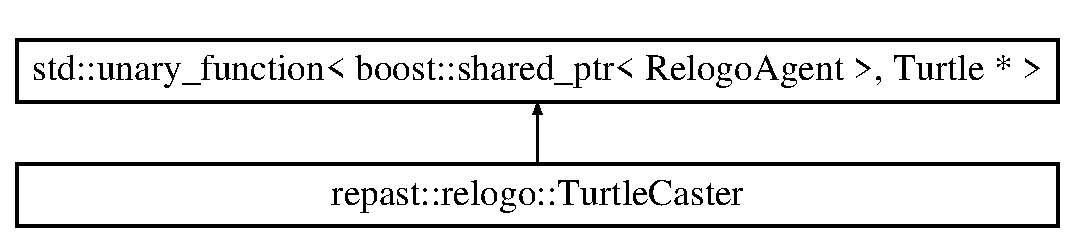
\includegraphics[height=2.000000cm]{structrepast_1_1relogo_1_1_turtle_caster}
\end{center}
\end{figure}
\subsection*{Public Member Functions}
\begin{DoxyCompactItemize}
\item 
\hypertarget{structrepast_1_1relogo_1_1_turtle_caster_add4a29ddb40cbe28574689d9f5212a1e}{\hyperlink{classrepast_1_1relogo_1_1_turtle}{Turtle} $\ast$ {\bfseries operator()} (boost\-::shared\-\_\-ptr$<$ \hyperlink{classrepast_1_1relogo_1_1_relogo_agent}{Relogo\-Agent} $>$ ptr) const }\label{structrepast_1_1relogo_1_1_turtle_caster_add4a29ddb40cbe28574689d9f5212a1e}

\end{DoxyCompactItemize}


\subsection{Detailed Description}
Casts a pointer to a \hyperlink{classrepast_1_1relogo_1_1_relogo_agent}{Relogo\-Agent} to a pointer to a \hyperlink{classrepast_1_1relogo_1_1_turtle}{Turtle}. 

The documentation for this struct was generated from the following file\-:\begin{DoxyCompactItemize}
\item 
/\-Users/murphy/work/\-Repast\-H\-P\-C\-\_\-\-G\-I\-T/repast.\-hpc/src/relogo/Observer.\-cpp\end{DoxyCompactItemize}

\hypertarget{structrepast_1_1relogo_1_1_type_info_cmp}{\section{repast\-:\-:relogo\-:\-:Type\-Info\-Cmp Struct Reference}
\label{structrepast_1_1relogo_1_1_type_info_cmp}\index{repast\-::relogo\-::\-Type\-Info\-Cmp@{repast\-::relogo\-::\-Type\-Info\-Cmp}}
}


Compare two elements of type std\-::type\-\_\-info using 'before'.  




{\ttfamily \#include $<$Observer.\-h$>$}

\subsection*{Public Member Functions}
\begin{DoxyCompactItemize}
\item 
\hypertarget{structrepast_1_1relogo_1_1_type_info_cmp_a4f70174d8421af1c26beb5ae9eb5059e}{bool {\bfseries operator()} (const std\-::type\-\_\-info $\ast$one, const std\-::type\-\_\-info $\ast$two) const }\label{structrepast_1_1relogo_1_1_type_info_cmp_a4f70174d8421af1c26beb5ae9eb5059e}

\end{DoxyCompactItemize}


\subsection{Detailed Description}
Compare two elements of type std\-::type\-\_\-info using 'before'. 

The documentation for this struct was generated from the following file\-:\begin{DoxyCompactItemize}
\item 
/\-Users/murphy/work/\-Repast\-H\-P\-C\-\_\-\-G\-I\-T/repast.\-hpc/src/relogo/Observer.\-h\end{DoxyCompactItemize}

\hypertarget{classrepast_1_1relogo_1_1_world_creator}{\section{repast\-:\-:relogo\-:\-:World\-Creator Class Reference}
\label{classrepast_1_1relogo_1_1_world_creator}\index{repast\-::relogo\-::\-World\-Creator@{repast\-::relogo\-::\-World\-Creator}}
}


Creates a the relogo world given some parameters.  




{\ttfamily \#include $<$World\-Creator.\-h$>$}

\subsection*{Public Member Functions}
\begin{DoxyCompactItemize}
\item 
\hypertarget{classrepast_1_1relogo_1_1_world_creator_ad664f192bb1909995b5df1b195487266}{{\bfseries World\-Creator} (boost\-::mpi\-::communicator $\ast$world)}\label{classrepast_1_1relogo_1_1_world_creator_ad664f192bb1909995b5df1b195487266}

\item 
{\footnotesize template$<$typename Obs\-Type , typename Patch\-Type , typename Patch\-Creator $>$ }\\Obs\-Type $\ast$ \hyperlink{classrepast_1_1relogo_1_1_world_creator_a61ef4601065168dfc0fc7fbf4d47e181}{create\-World} (const \hyperlink{classrepast_1_1relogo_1_1_world_definition}{World\-Definition} \&world\-Def, const std\-::vector$<$ int $>$ \&p\-Config, Patch\-Creator \&patch\-Creator)
\begin{DoxyCompactList}\small\item\em Creates the Relogo world using the specified parameters and returns an \hyperlink{classrepast_1_1relogo_1_1_observer}{Observer} of Obs\-Type. \end{DoxyCompactList}\item 
{\footnotesize template$<$typename Obs\-Type , typename Patch\-Type $>$ }\\Obs\-Type $\ast$ \hyperlink{classrepast_1_1relogo_1_1_world_creator_aaceddc663139a0fda80b3022e0cd0d08}{create\-World} (const \hyperlink{classrepast_1_1relogo_1_1_world_definition}{World\-Definition} \&world\-Def, const std\-::vector$<$ int $>$ \&p\-Config)
\begin{DoxyCompactList}\small\item\em Creates an observer of the specified type. \end{DoxyCompactList}\end{DoxyCompactItemize}


\subsection{Detailed Description}
Creates a the relogo world given some parameters. 

\subsection{Member Function Documentation}
\hypertarget{classrepast_1_1relogo_1_1_world_creator_a61ef4601065168dfc0fc7fbf4d47e181}{\index{repast\-::relogo\-::\-World\-Creator@{repast\-::relogo\-::\-World\-Creator}!create\-World@{create\-World}}
\index{create\-World@{create\-World}!repast::relogo::WorldCreator@{repast\-::relogo\-::\-World\-Creator}}
\subsubsection[{create\-World}]{\setlength{\rightskip}{0pt plus 5cm}template$<$typename Obs\-Type , typename Patch\-Type , typename Patch\-Creator $>$ Obs\-Type $\ast$ repast\-::relogo\-::\-World\-Creator\-::create\-World (
\begin{DoxyParamCaption}
\item[{const {\bf World\-Definition} \&}]{world\-Def, }
\item[{const std\-::vector$<$ int $>$ \&}]{p\-Config, }
\item[{Patch\-Creator \&}]{patch\-Creator}
\end{DoxyParamCaption}
)}}\label{classrepast_1_1relogo_1_1_world_creator_a61ef4601065168dfc0fc7fbf4d47e181}


Creates the Relogo world using the specified parameters and returns an \hyperlink{classrepast_1_1relogo_1_1_observer}{Observer} of Obs\-Type. 


\begin{DoxyParams}{Parameters}
{\em world\-Def} & the world definition \\
\hline
{\em p\-Config} & a two element vector describing the number of processes along the x and y dimensions \\
\hline
{\em patch\-Creator} & used to create the Patches.\\
\hline
\end{DoxyParams}

\begin{DoxyTemplParams}{Template Parameters}
{\em Obs\-Type} & the type of \hyperlink{classrepast_1_1relogo_1_1_observer}{Observer} to create. This must extend \hyperlink{classrepast_1_1relogo_1_1_observer}{Observer}. \\
\hline
{\em Patch\-Type} & the type of Patches to create. This must either be or extend \hyperlink{classrepast_1_1relogo_1_1_patch}{Patch}. \\
\hline
{\em Patch\-Creator} & a function or functor with the following signature Patch\-Type$\ast$ (Agent\-Id id, Observer$\ast$ obs). \\
\hline
\end{DoxyTemplParams}
\hypertarget{classrepast_1_1relogo_1_1_world_creator_aaceddc663139a0fda80b3022e0cd0d08}{\index{repast\-::relogo\-::\-World\-Creator@{repast\-::relogo\-::\-World\-Creator}!create\-World@{create\-World}}
\index{create\-World@{create\-World}!repast::relogo::WorldCreator@{repast\-::relogo\-::\-World\-Creator}}
\subsubsection[{create\-World}]{\setlength{\rightskip}{0pt plus 5cm}template$<$typename Obs\-Type , typename Patch\-Type $>$ Obs\-Type $\ast$ repast\-::relogo\-::\-World\-Creator\-::create\-World (
\begin{DoxyParamCaption}
\item[{const {\bf World\-Definition} \&}]{world\-Def, }
\item[{const std\-::vector$<$ int $>$ \&}]{p\-Config}
\end{DoxyParamCaption}
)}}\label{classrepast_1_1relogo_1_1_world_creator_aaceddc663139a0fda80b3022e0cd0d08}


Creates an observer of the specified type. 

The observer will contain a world defined by world\-Def and p\-Config.


\begin{DoxyParams}{Parameters}
{\em world\-Def} & the world definition \\
\hline
{\em p\-Config} & a 2\-D vector containing the number of processes per grid dimension\\
\hline
\end{DoxyParams}

\begin{DoxyTemplParams}{Template Parameters}
{\em Obs\-Type} & the type of \hyperlink{classrepast_1_1relogo_1_1_observer}{Observer} to create. This must extend \hyperlink{classrepast_1_1relogo_1_1_observer}{Observer}. \\
\hline
{\em Patch\-Type} & the type of Patches to create. This must either be or extend \hyperlink{classrepast_1_1relogo_1_1_patch}{Patch}. \\
\hline
\end{DoxyTemplParams}


The documentation for this class was generated from the following files\-:\begin{DoxyCompactItemize}
\item 
/\-Users/murphy/work/\-Repast\-H\-P\-C\-\_\-\-G\-I\-T/repast.\-hpc/src/relogo/World\-Creator.\-h\item 
/\-Users/murphy/work/\-Repast\-H\-P\-C\-\_\-\-G\-I\-T/repast.\-hpc/src/relogo/World\-Creator.\-cpp\end{DoxyCompactItemize}

\hypertarget{classrepast_1_1relogo_1_1_world_definition}{\section{repast\-:\-:relogo\-:\-:World\-Definition Class Reference}
\label{classrepast_1_1relogo_1_1_world_definition}\index{repast\-::relogo\-::\-World\-Definition@{repast\-::relogo\-::\-World\-Definition}}
}


Defines a Relogo world.  




{\ttfamily \#include $<$World\-Definition.\-h$>$}

\subsection*{Public Types}
\begin{DoxyCompactItemize}
\item 
\hypertarget{classrepast_1_1relogo_1_1_world_definition_ab1e044b19b6cb8c2e00110e48882afcc}{typedef std\-::vector\\*
$<$ Projection$<$ \hyperlink{classrepast_1_1relogo_1_1_relogo_agent}{Relogo\-Agent} $>$\\*
 $\ast$ $>$\-::const\-\_\-iterator \hyperlink{classrepast_1_1relogo_1_1_world_definition_ab1e044b19b6cb8c2e00110e48882afcc}{proj\-\_\-iter}}\label{classrepast_1_1relogo_1_1_world_definition_ab1e044b19b6cb8c2e00110e48882afcc}

\begin{DoxyCompactList}\small\item\em An iterator over pointers to Projection$<$\-Relogo\-Agent$>$. \end{DoxyCompactList}\end{DoxyCompactItemize}
\subsection*{Public Member Functions}
\begin{DoxyCompactItemize}
\item 
\hyperlink{classrepast_1_1relogo_1_1_world_definition_a6652b63cad8c22f1ad7aac7e5be87587}{World\-Definition} (int \hyperlink{classrepast_1_1relogo_1_1_world_definition_a952ccd4e18c655e3242bdc7d32e062d1}{min\-X}, int \hyperlink{classrepast_1_1relogo_1_1_world_definition_a225c0ad83e73e13e5e5a55226ffa1dbb}{min\-Y}, int \hyperlink{classrepast_1_1relogo_1_1_world_definition_a08eb3fa1fd9d6aed840f713d23b9ff48}{max\-X}, int \hyperlink{classrepast_1_1relogo_1_1_world_definition_a3395109e5074f8bacbbd0bb0fa36f089}{max\-Y}, bool wrapped, int \hyperlink{classrepast_1_1relogo_1_1_world_definition_aa02082d00b9badcf1e3894dbdc08b586}{buffer})
\begin{DoxyCompactList}\small\item\em Creates a world definition with the specified parameters. \end{DoxyCompactList}\item 
void \hyperlink{classrepast_1_1relogo_1_1_world_definition_af0dbe714030627a4274831f9bfe7f847}{define\-Network} (std\-::string name, bool directed, \hyperlink{classrepast_1_1relogo_1_1_relogo_link_content_manager}{Relogo\-Link\-Content\-Manager} $\ast$rlcm)
\begin{DoxyCompactList}\small\item\em Defines a network with the specified name and whether or not the network is directed. \end{DoxyCompactList}\item 
void \hyperlink{classrepast_1_1relogo_1_1_world_definition_a99d9ec41613be3c9ac9c9604b5030225}{define\-Network} (bool directed, \hyperlink{classrepast_1_1relogo_1_1_relogo_link_content_manager}{Relogo\-Link\-Content\-Manager} $\ast$rlcm)
\begin{DoxyCompactList}\small\item\em Defines the default network and whether or not the network is directed. \end{DoxyCompactList}\item 
\hyperlink{classrepast_1_1relogo_1_1_world_definition_ab1e044b19b6cb8c2e00110e48882afcc}{proj\-\_\-iter} \hyperlink{classrepast_1_1relogo_1_1_world_definition_a6e5b0f7af7876b41a5e5a8a69e43f615}{networks\-\_\-begin} () const 
\begin{DoxyCompactList}\small\item\em Gets the start of an iterator over the network Projections defined in this \hyperlink{classrepast_1_1relogo_1_1_world_definition}{World\-Definition}. \end{DoxyCompactList}\item 
\hyperlink{classrepast_1_1relogo_1_1_world_definition_ab1e044b19b6cb8c2e00110e48882afcc}{proj\-\_\-iter} \hyperlink{classrepast_1_1relogo_1_1_world_definition_a0bd3c542fb88b54f4c0c821fbf6008c4}{networks\-\_\-end} () const 
\begin{DoxyCompactList}\small\item\em Gets the end of an iterator over the network Projections defined in this \hyperlink{classrepast_1_1relogo_1_1_world_definition}{World\-Definition}. \end{DoxyCompactList}\item 
int \hyperlink{classrepast_1_1relogo_1_1_world_definition_a952ccd4e18c655e3242bdc7d32e062d1}{min\-X} () const 
\begin{DoxyCompactList}\small\item\em Gets the minimum x coordinate of the world. \end{DoxyCompactList}\item 
int \hyperlink{classrepast_1_1relogo_1_1_world_definition_a225c0ad83e73e13e5e5a55226ffa1dbb}{min\-Y} () const 
\begin{DoxyCompactList}\small\item\em Gets the minimum y coordinate of the world. \end{DoxyCompactList}\item 
int \hyperlink{classrepast_1_1relogo_1_1_world_definition_a08eb3fa1fd9d6aed840f713d23b9ff48}{max\-X} () const 
\begin{DoxyCompactList}\small\item\em Gets the maximum x coordinate of the world. \end{DoxyCompactList}\item 
int \hyperlink{classrepast_1_1relogo_1_1_world_definition_a3395109e5074f8bacbbd0bb0fa36f089}{max\-Y} () const 
\begin{DoxyCompactList}\small\item\em Gets the maximum y coordinate of the world. \end{DoxyCompactList}\item 
const Grid\-Dimensions \hyperlink{classrepast_1_1relogo_1_1_world_definition_a9fe209e15771261f76b7b793477e896f}{dimensions} () const 
\begin{DoxyCompactList}\small\item\em Gets the dimensions of the world expressed as a Grid\-Dimensions. \end{DoxyCompactList}\item 
bool \hyperlink{classrepast_1_1relogo_1_1_world_definition_a86887fe5eb38619d16388c27aa2688f2}{is\-Wrapped} () const 
\begin{DoxyCompactList}\small\item\em Gets whether or not the world wraps. \end{DoxyCompactList}\item 
int \hyperlink{classrepast_1_1relogo_1_1_world_definition_aa02082d00b9badcf1e3894dbdc08b586}{buffer} () const 
\begin{DoxyCompactList}\small\item\em Gets the size of the grid / space buffer. \end{DoxyCompactList}\end{DoxyCompactItemize}


\subsection{Detailed Description}
Defines a Relogo world. 

\subsection{Constructor \& Destructor Documentation}
\hypertarget{classrepast_1_1relogo_1_1_world_definition_a6652b63cad8c22f1ad7aac7e5be87587}{\index{repast\-::relogo\-::\-World\-Definition@{repast\-::relogo\-::\-World\-Definition}!World\-Definition@{World\-Definition}}
\index{World\-Definition@{World\-Definition}!repast::relogo::WorldDefinition@{repast\-::relogo\-::\-World\-Definition}}
\subsubsection[{World\-Definition}]{\setlength{\rightskip}{0pt plus 5cm}repast\-::relogo\-::\-World\-Definition\-::\-World\-Definition (
\begin{DoxyParamCaption}
\item[{int}]{min\-X, }
\item[{int}]{min\-Y, }
\item[{int}]{max\-X, }
\item[{int}]{max\-Y, }
\item[{bool}]{wrapped, }
\item[{int}]{buffer}
\end{DoxyParamCaption}
)}}\label{classrepast_1_1relogo_1_1_world_definition_a6652b63cad8c22f1ad7aac7e5be87587}


Creates a world definition with the specified parameters. 

These parameter will be applied when the world is created using a \hyperlink{classrepast_1_1relogo_1_1_world_creator}{World\-Creator}.


\begin{DoxyParams}{Parameters}
{\em min\-X} & the minimum x coordinate of the world \\
\hline
{\em min\-Y} & the minimum y coordinate of the world \\
\hline
{\em max\-X} & the maximum x coordinate of the world \\
\hline
{\em max\-Y} & the maximum y coordinate of the world \\
\hline
{\em wrapped} & whether or not the space is periodic, wrapped as a torus \\
\hline
{\em buffer} & the size of the grid and space buffer between process grid and space representations \\
\hline
\end{DoxyParams}


\subsection{Member Function Documentation}
\hypertarget{classrepast_1_1relogo_1_1_world_definition_aa02082d00b9badcf1e3894dbdc08b586}{\index{repast\-::relogo\-::\-World\-Definition@{repast\-::relogo\-::\-World\-Definition}!buffer@{buffer}}
\index{buffer@{buffer}!repast::relogo::WorldDefinition@{repast\-::relogo\-::\-World\-Definition}}
\subsubsection[{buffer}]{\setlength{\rightskip}{0pt plus 5cm}int repast\-::relogo\-::\-World\-Definition\-::buffer (
\begin{DoxyParamCaption}
{}
\end{DoxyParamCaption}
) const\hspace{0.3cm}{\ttfamily [inline]}}}\label{classrepast_1_1relogo_1_1_world_definition_aa02082d00b9badcf1e3894dbdc08b586}


Gets the size of the grid / space buffer. 

\begin{DoxyReturn}{Returns}
the size of the grid / space buffer. 
\end{DoxyReturn}
\hypertarget{classrepast_1_1relogo_1_1_world_definition_af0dbe714030627a4274831f9bfe7f847}{\index{repast\-::relogo\-::\-World\-Definition@{repast\-::relogo\-::\-World\-Definition}!define\-Network@{define\-Network}}
\index{define\-Network@{define\-Network}!repast::relogo::WorldDefinition@{repast\-::relogo\-::\-World\-Definition}}
\subsubsection[{define\-Network}]{\setlength{\rightskip}{0pt plus 5cm}void repast\-::relogo\-::\-World\-Definition\-::define\-Network (
\begin{DoxyParamCaption}
\item[{std\-::string}]{name, }
\item[{bool}]{directed, }
\item[{{\bf Relogo\-Link\-Content\-Manager} $\ast$}]{rlcm}
\end{DoxyParamCaption}
)}}\label{classrepast_1_1relogo_1_1_world_definition_af0dbe714030627a4274831f9bfe7f847}


Defines a network with the specified name and whether or not the network is directed. 

The network will use the default Relogo\-Edge.


\begin{DoxyParams}{Parameters}
{\em name} & the name of the network \\
\hline
{\em directed} & if true, the network will be directed, otherwise it will be undirected \\
\hline
\end{DoxyParams}
\hypertarget{classrepast_1_1relogo_1_1_world_definition_a99d9ec41613be3c9ac9c9604b5030225}{\index{repast\-::relogo\-::\-World\-Definition@{repast\-::relogo\-::\-World\-Definition}!define\-Network@{define\-Network}}
\index{define\-Network@{define\-Network}!repast::relogo::WorldDefinition@{repast\-::relogo\-::\-World\-Definition}}
\subsubsection[{define\-Network}]{\setlength{\rightskip}{0pt plus 5cm}void repast\-::relogo\-::\-World\-Definition\-::define\-Network (
\begin{DoxyParamCaption}
\item[{bool}]{directed, }
\item[{{\bf Relogo\-Link\-Content\-Manager} $\ast$}]{rlcm}
\end{DoxyParamCaption}
)}}\label{classrepast_1_1relogo_1_1_world_definition_a99d9ec41613be3c9ac9c9604b5030225}


Defines the default network and whether or not the network is directed. 

Any network related calls that don't specify a name will use this network. The network will use Relogo\-Edge-\/s by default


\begin{DoxyParams}{Parameters}
{\em directed} & if true, the network will be directed, otherwise it will be undirected \\
\hline
\end{DoxyParams}
\hypertarget{classrepast_1_1relogo_1_1_world_definition_a9fe209e15771261f76b7b793477e896f}{\index{repast\-::relogo\-::\-World\-Definition@{repast\-::relogo\-::\-World\-Definition}!dimensions@{dimensions}}
\index{dimensions@{dimensions}!repast::relogo::WorldDefinition@{repast\-::relogo\-::\-World\-Definition}}
\subsubsection[{dimensions}]{\setlength{\rightskip}{0pt plus 5cm}const Grid\-Dimensions repast\-::relogo\-::\-World\-Definition\-::dimensions (
\begin{DoxyParamCaption}
{}
\end{DoxyParamCaption}
) const\hspace{0.3cm}{\ttfamily [inline]}}}\label{classrepast_1_1relogo_1_1_world_definition_a9fe209e15771261f76b7b793477e896f}


Gets the dimensions of the world expressed as a Grid\-Dimensions. 

\begin{DoxyReturn}{Returns}
the dimensions of the world expressed as a Grid\-Dimensions. 
\end{DoxyReturn}
\hypertarget{classrepast_1_1relogo_1_1_world_definition_a86887fe5eb38619d16388c27aa2688f2}{\index{repast\-::relogo\-::\-World\-Definition@{repast\-::relogo\-::\-World\-Definition}!is\-Wrapped@{is\-Wrapped}}
\index{is\-Wrapped@{is\-Wrapped}!repast::relogo::WorldDefinition@{repast\-::relogo\-::\-World\-Definition}}
\subsubsection[{is\-Wrapped}]{\setlength{\rightskip}{0pt plus 5cm}bool repast\-::relogo\-::\-World\-Definition\-::is\-Wrapped (
\begin{DoxyParamCaption}
{}
\end{DoxyParamCaption}
) const\hspace{0.3cm}{\ttfamily [inline]}}}\label{classrepast_1_1relogo_1_1_world_definition_a86887fe5eb38619d16388c27aa2688f2}


Gets whether or not the world wraps. 

\begin{DoxyReturn}{Returns}
true if the world wraps, otherwise false. 
\end{DoxyReturn}
\hypertarget{classrepast_1_1relogo_1_1_world_definition_a08eb3fa1fd9d6aed840f713d23b9ff48}{\index{repast\-::relogo\-::\-World\-Definition@{repast\-::relogo\-::\-World\-Definition}!max\-X@{max\-X}}
\index{max\-X@{max\-X}!repast::relogo::WorldDefinition@{repast\-::relogo\-::\-World\-Definition}}
\subsubsection[{max\-X}]{\setlength{\rightskip}{0pt plus 5cm}int repast\-::relogo\-::\-World\-Definition\-::max\-X (
\begin{DoxyParamCaption}
{}
\end{DoxyParamCaption}
) const\hspace{0.3cm}{\ttfamily [inline]}}}\label{classrepast_1_1relogo_1_1_world_definition_a08eb3fa1fd9d6aed840f713d23b9ff48}


Gets the maximum x coordinate of the world. 

\begin{DoxyReturn}{Returns}
the maximum x coordinate of the world. 
\end{DoxyReturn}
\hypertarget{classrepast_1_1relogo_1_1_world_definition_a3395109e5074f8bacbbd0bb0fa36f089}{\index{repast\-::relogo\-::\-World\-Definition@{repast\-::relogo\-::\-World\-Definition}!max\-Y@{max\-Y}}
\index{max\-Y@{max\-Y}!repast::relogo::WorldDefinition@{repast\-::relogo\-::\-World\-Definition}}
\subsubsection[{max\-Y}]{\setlength{\rightskip}{0pt plus 5cm}int repast\-::relogo\-::\-World\-Definition\-::max\-Y (
\begin{DoxyParamCaption}
{}
\end{DoxyParamCaption}
) const\hspace{0.3cm}{\ttfamily [inline]}}}\label{classrepast_1_1relogo_1_1_world_definition_a3395109e5074f8bacbbd0bb0fa36f089}


Gets the maximum y coordinate of the world. 

\begin{DoxyReturn}{Returns}
the maximum y coordinate of the world. 
\end{DoxyReturn}
\hypertarget{classrepast_1_1relogo_1_1_world_definition_a952ccd4e18c655e3242bdc7d32e062d1}{\index{repast\-::relogo\-::\-World\-Definition@{repast\-::relogo\-::\-World\-Definition}!min\-X@{min\-X}}
\index{min\-X@{min\-X}!repast::relogo::WorldDefinition@{repast\-::relogo\-::\-World\-Definition}}
\subsubsection[{min\-X}]{\setlength{\rightskip}{0pt plus 5cm}int repast\-::relogo\-::\-World\-Definition\-::min\-X (
\begin{DoxyParamCaption}
{}
\end{DoxyParamCaption}
) const\hspace{0.3cm}{\ttfamily [inline]}}}\label{classrepast_1_1relogo_1_1_world_definition_a952ccd4e18c655e3242bdc7d32e062d1}


Gets the minimum x coordinate of the world. 

\begin{DoxyReturn}{Returns}
the minimum x coordinate of the world. 
\end{DoxyReturn}
\hypertarget{classrepast_1_1relogo_1_1_world_definition_a225c0ad83e73e13e5e5a55226ffa1dbb}{\index{repast\-::relogo\-::\-World\-Definition@{repast\-::relogo\-::\-World\-Definition}!min\-Y@{min\-Y}}
\index{min\-Y@{min\-Y}!repast::relogo::WorldDefinition@{repast\-::relogo\-::\-World\-Definition}}
\subsubsection[{min\-Y}]{\setlength{\rightskip}{0pt plus 5cm}int repast\-::relogo\-::\-World\-Definition\-::min\-Y (
\begin{DoxyParamCaption}
{}
\end{DoxyParamCaption}
) const\hspace{0.3cm}{\ttfamily [inline]}}}\label{classrepast_1_1relogo_1_1_world_definition_a225c0ad83e73e13e5e5a55226ffa1dbb}


Gets the minimum y coordinate of the world. 

\begin{DoxyReturn}{Returns}
the minimum y coordinate of the world. 
\end{DoxyReturn}
\hypertarget{classrepast_1_1relogo_1_1_world_definition_a6e5b0f7af7876b41a5e5a8a69e43f615}{\index{repast\-::relogo\-::\-World\-Definition@{repast\-::relogo\-::\-World\-Definition}!networks\-\_\-begin@{networks\-\_\-begin}}
\index{networks\-\_\-begin@{networks\-\_\-begin}!repast::relogo::WorldDefinition@{repast\-::relogo\-::\-World\-Definition}}
\subsubsection[{networks\-\_\-begin}]{\setlength{\rightskip}{0pt plus 5cm}{\bf proj\-\_\-iter} repast\-::relogo\-::\-World\-Definition\-::networks\-\_\-begin (
\begin{DoxyParamCaption}
{}
\end{DoxyParamCaption}
) const\hspace{0.3cm}{\ttfamily [inline]}}}\label{classrepast_1_1relogo_1_1_world_definition_a6e5b0f7af7876b41a5e5a8a69e43f615}


Gets the start of an iterator over the network Projections defined in this \hyperlink{classrepast_1_1relogo_1_1_world_definition}{World\-Definition}. 

The iterator returns a pointer to a Projection$<$\-Relogo\-Agent$>$$\ast$. \hypertarget{classrepast_1_1relogo_1_1_world_definition_a0bd3c542fb88b54f4c0c821fbf6008c4}{\index{repast\-::relogo\-::\-World\-Definition@{repast\-::relogo\-::\-World\-Definition}!networks\-\_\-end@{networks\-\_\-end}}
\index{networks\-\_\-end@{networks\-\_\-end}!repast::relogo::WorldDefinition@{repast\-::relogo\-::\-World\-Definition}}
\subsubsection[{networks\-\_\-end}]{\setlength{\rightskip}{0pt plus 5cm}{\bf proj\-\_\-iter} repast\-::relogo\-::\-World\-Definition\-::networks\-\_\-end (
\begin{DoxyParamCaption}
{}
\end{DoxyParamCaption}
) const\hspace{0.3cm}{\ttfamily [inline]}}}\label{classrepast_1_1relogo_1_1_world_definition_a0bd3c542fb88b54f4c0c821fbf6008c4}


Gets the end of an iterator over the network Projections defined in this \hyperlink{classrepast_1_1relogo_1_1_world_definition}{World\-Definition}. 

The iterator returns a pointer to a Projection$<$\-Relogo\-Agent$>$$\ast$. 

The documentation for this class was generated from the following files\-:\begin{DoxyCompactItemize}
\item 
/\-Users/murphy/work/\-Repast\-H\-P\-C\-\_\-\-G\-I\-T/repast.\-hpc/src/relogo/World\-Definition.\-h\item 
/\-Users/murphy/work/\-Repast\-H\-P\-C\-\_\-\-G\-I\-T/repast.\-hpc/src/relogo/World\-Definition.\-cpp\end{DoxyCompactItemize}

%--- End generated contents ---

% Index
\newpage
\phantomsection
\addcontentsline{toc}{part}{Index}
\printindex

\end{document}
